% Source code for PSOPT manual
% Author: Victor M. Becerra
%
%


\documentclass[a4paper,11pt]{report}    % Specifies the document style.
\bibliographystyle{plain}



\usepackage{framed,fancybox}
\usepackage{verbatim}
\usepackage[pdftex,colorlinks]{hyperref}
\hypersetup{%
colorlinks=true,
linkcolor=blue,
urlcolor=magenta
}%



\renewcommand{\bibname}{References}

\newcommand{\psopt}{$\mathcal{PSOPT}$\,}  %  

\newcommand{\release}{Release 4 \,}

\newcommand{\build}{build 2015 \,}

\newcommand{\basedir}{\texttt{psopt-master\,}}



\usepackage{epsfig}
\usepackage{graphicx}
\usepackage{amssymb,amsfonts}
\usepackage{amsmath}
\usepackage{amsbsy}


\newcommand{\RE}{\mathcal{R}}

\newcommand{\mt}[1]{\ensuremath \mathbf{#1}}

\newcommand{\shell}[1]{\$ \texttt{#1}\\}
\newcommand{\shellcont}[1]{\texttt{#1}\\}

\usepackage{color}

\definecolor{shadecolor}{gray}{0.97}
\FrameRule=0.75pt
\FrameSep=5pt
\setlength{\fboxrule}{\FrameRule}
\setlength{\fboxsep}{\FrameSep}



\newenvironment{shadedframe}{%
  \def\FrameCommand{\fcolorbox{black}{shadecolor}}%
%  \MakeFramed {\addtolength{\hsize}{-\width}\FrameRestore}}
  \MakeFramed {\FrameRestore}}
{\endMakeFramed}


\begin{document}

\title{\psopt Optimal Control Solver\\ User Manual \\ \small \release \build \normalsize }

\author{Victor M. Becerra \\ Email: v.m.becerra@ieee.org  \\ http://www.psopt.org}

\date{Copyright \copyright \,\, 2012 Victor M. Becerra}


\maketitle

\chapter*{Disclaimer}

This software is provided ``as is'' and is distributed free of charge. It comes with
no warrantees of any kind. See the license terms
for more details.  The author does hope, however, that users 
will find this software useful for research and other purposes. 

\chapter*{Licensing Agreement}
The software package \psopt is distributed under the GNU Lesser General Public License version 2.1.
Users of the software must abide by the terms of the license.

\scriptsize
\begin{shadedframe}
\verbatiminput{../LICENSE.txt}
\end{shadedframe}
\normalsize


\tableofcontents

%%%%%%%%%%%%%%%%%%%%%%%%%%%%%%%%%%%%%%%%%%%%%%%%%%%%%%%%%%%%%%%%%%%

\chapter{Introduction to \psopt}

\section{What is \psopt}

\psopt is an open source optimal control package written in C++ that uses direct collocation methods. 
These methods solve optimal control problems by approximating the time-dependent variables using global or local polynomials.
This allows to discretize the differential equations and continuous constraints
over a grid of nodes, and to compute any integrals associated with the problem using well known quadrature formulas. 
Nonlinear programming then is used to find local optimal
solutions. \psopt is able to deal with problems with the following characteristics:

\begin{itemize}
 \item Single or multiphase problems
 \item Continuous time nonlinear dynamics
 \item General endpoint constraints
 \item Nonlinear path constraints (equalities or inequalities) on states and/or control variables
 \item Integral constraints
 \item Interior point constraints
 \item Bounds on controls and state variables
 \item General cost function with Lagrange and Mayer terms.
 \item Free or fixed initial and final conditions
 \item Linear or nonlinear linkages between phases
 \item Fixed or free initial time
 \item Fixed or free final time
 \item Optimisation of static parameters
 \item Parameter estimation problems with sampled measurements
 \item Differential equations with delayed variables.
\end{itemize}

The implementation has the following features:

\begin{itemize}
 \item Automatic scaling
 \item Automatic first and second derivatives using the ADOL-C library
 \item Numerical differentiation by using sparse finite differences
 \item Automatic mesh refinement
 \item Automatic identification of the Jacobian and Hessian sparsity.
 \item DAE formulation, so that differential and algebraic constraints 
       can be implemented in the same C++ function.
\end{itemize}

\psopt has interfaces to the following NLP solvers:

\begin{itemize}
 \item IPOPT: an open source C++ implementation of an interior point method for large scale problems.
 \item SNOPT: a well known and widely used proprietary large scale NLP solver.
\end{itemize}

\subsection{Why use \psopt and what alternatives exist}

These are
some reasons why users may wish to use \psopt:

\begin{itemize}
\item Users who for any reason do not have access to commercial optimal control solvers
and wish to employ a free open source package for optimal control which does not
need a proprietary software environment to run.
\item Users who need to link an optimal control solver from  stand alone applications written
in C++ or other programming languages.
\item Users who want to do research with the software, for instance by implementing
their own problems, or by customising the code.
\end{itemize}

\psopt does not require a commercial software environment to run on, 
or to be compiled. \psopt is fully compatible with the \texttt{gcc} compiler, and has
been developed under Linux, a free operating system.
Note also that the default NLP solver (IPOPT) requires a sparse linear solver
from a range of options, some of which are available at no cost. The author has personally 
used the linear solver \texttt{ma27}. 

\psopt has also been ported to be compiled by Microsoft Visual Studio 2010 under Windows 7.

At the time of writing, there is at least one freely available tool implementing 
a pseudospectral optimal control method. This is GPOPS \cite{Rao:08}, which has been
developed by Anil Rao (University of Florida) and co-workers. GPOPS
uses a Gauss pseudospectral method and requires \textsc{Matlab} and SNOPT. GPOPS
can be downloaded from: 
\begin{center}
\href{http://sourceforge.net/projects/gpops/}{http://sourceforge.net/projects/gpops/}
\end{center}

There are commercial tools for solving large scale optimal control problems. Some
modern commercial tools include:
\begin{itemize}
\item SOCS developed by J.T. Betts from  Boeing,  which is a well known tool that is
able to solve very large optimal control problems and uses a direct transcription  method. See:
\begin{center}
\href{http://www.boeing.com/phantom/socs/}{http://www.boeing.com/phantom/socs/}
\end{center}

\item GESOP developed by Astos Solutions GmbH, Germany,  which uses various methods for solving complex optimal control problems
and includes a graphical user interface. See:
\begin{center}
\href{http://www.astos.de/products/gesop}{http://www.astos.de/products/gesop}
\end{center}

 \item  PROPT, developed by P. E.  Rutquist and M. M. Edvall from Tomlab Optimization, which runs under \textsc{Matlab} and
uses pseudospectral methods. See:

\begin{center}
\href{http://www.tomdyn.com}{http://www.tomdyn.com}
\end{center}
 \item DIDO, developed by I.M. Ross from the Postgraduate Naval School
in Monterey, California,  is a package that runs under \textsc{Matlab} and uses pseudospectral methods. See:

\begin{center}
 \href{http://www.elissar.biz/DIDO.html}{http://www.elissar.biz/DIDO.html}
\end{center}



\end{itemize}

Other software tools implementing direct transcription methods for optimal control include:

\begin{itemize}
 \item DIRCOL , authored by O. von Stryk, which is a Fortran 77 based tool that uses a direct collocation method. See:
\begin{center}
 \href{http://www.sim.informatik.tu-darmstadt.de/sw/dircol/dircol.html}{http://www.sim.informatik.tu-darmstadt.de/sw/dircol/dircol.html}
\end{center}

 \item DYNOPT, authored by M. Fikar and M. Cizniar, which is a \textsc{Matlab} based
tool that uses orthogonal collocation on finite elements. See:
\begin{center}
\href{http://www.kirp.chtf.stuba.sk/~fikar/research/dynopt/dynopt.htm}{http://www.kirp.chtf.stuba.sk/~fikar/research/dynopt/dynopt.htm}
\end{center}

\end{itemize}

\section{\psopt user's group}

A user's group has been created with the purpose of enabling users to share their experiences with using \psopt, 
and to keep a public record of exchanges with the author. It is also a way of being informed about the latest
developments with \psopt and to ask for help. Membership is free and open. The  \psopt user's group is located at:

\href{http://groups.google.com/group/psopt-users-group}{http://groups.google.com/group/psopt-users-group}



\subsection{About the author}

Victor M. Becerra obtained his first degree in Electrical Engineering in 1990 from Simon Bolivar
University, Caracas Venezuela. Between 1989 and 1991 he worked in power systems analysis in CVG Edelca,
Caracas. He obtained his PhD for his work on the development of nonlinear optimal control methods
from City University, London, in 1994.  Between 1994 and 1999 he was a Research Fellow at the Control
Engineering Research Centre at City University, London. He is currently a Reader in Cybernetics at the University of Reading, 
UK, where he has been an academic since 2000. At Reading, he lead the Cybernetics Intelligence Research Group
between 2003 and 2009, and currently manages the MSc in Cybernetics, a one year postgraduate programme which he founded. 
He is a Senior Member of the IEEE and a Member of the Institute of Engineering and Technology. 
He has published over 100 research papers and one book. His web site is: \href{http://www.reading.ac.uk/~shs99vmb}{http://www.reading.ac.uk/\~{}shs99vmb}.


\subsection{Contacting the author}


The author is open to discussing with users potential research collaboration 
leading to publications, academic exchanges, or joint projects. He can be contacted directly for help
on the installation and use of the software. Consultancy and training on the use of  \psopt are 
also available. His email address is:  \texttt{v.m.becerra@ieee.org}.




\subsection{How you can help}

You may help improve \psopt in a number of ways. 

\begin{itemize}
 \item  Sending bug reports.
 \item  Sending corrections to the documentation.
 \item  Discussing with the author ways to improve the computational aspects
        or capabilities  of the software.
 \item  Sending to the author proposed modifications to the source code, for consideration
        to be included in a future release of \psopt.
 \item  Sending source code with new examples which may be included (with due acknowledgement) in future releases of \psopt.
 \item  Porting the software to new architectures.
 \item  If you have had a good experience with \psopt, tell your students or colleagues
about it.
 \item  Quoting the use of \psopt in your scientific publications. This document may be referenced as follows:

\begin{itemize}
\item Becerra, V.M. (2010). "Solving complex optimal control problems at no cost with PSOPT". \textit{Proc. IEEE Multi-conference on Systems and Control}, Yokohama, Japan, September 7-10, 2010, pp. 1391-1396

\item Becerra, V.M. (2010). \textit{PSOPT Optimal Control Solver User Manual. Release 3}.  Available: \texttt{http://code.google.com/p/psopt/\\downloads/list}
\end{itemize}


 \item  Developing interfaces to other NLP solvers.
\end{itemize}



\section{What is new in Release 3}

\begin{enumerate}
 \item New interface to facilitate the definition of single or multi-phase parameter estimation problems involving
sampled observations.
 \item Support of newer versions of IPOPT and ADOL-C.
 \item Additional auxiliary functions, including 2-D interpolation functions.
 \item New function to generate multi-plots with GNUplot, this is multiple plots in a single window.
 \item Additional examples
 \item Miscellaneous improvements and bug fixing.


\end{enumerate}

\section{General problem formulation}

\psopt solves the following general optimal control problem with $N_p$ phases:

\subsection*{Problem $\mathcal{P}_1$} Find the control trajectories, $u^{(i)}(t), t\in [t_0^{(i)}, t_f^{(i)}]$, state trajectories $x^{(i)}(t), t\in [t_0^{(i)}, t_f^{(i)}]$, static parameters $p^{(i)}$, and 
times $t_0^{(i)}, t_f^{(i)}$, $i=1,\ldots,N_p$,  to minimise the following performance index:
\[
   J = \sum\limits_{i=1}^{N_p} \left[ \varphi^{(i)}[ x^{(i)}(t_f^{(i)}), p^{(i)}, t_f^{(i)} ] + \int_{t_0^{(i)}}^{t_f^{(i)}} L^{(i)}[x^{(i)}(t),u^{(i)}(t),p^{(i)},t] dt \right]
\]

\noindent subject to the differential constraints:
\[
 \dot x^{(i)}(t) = f^{(i)}[ x^{(i)}(t),u^{(i)}(t),p^{(i)},t ], \, \,t\in[t_0^{(i)},t_f^{(i)}],
\]
the path constraints
\[
 h_L^{(i)} \le h^{(i)}[ x^{(i)}(t),u^{(i)}(t),p^{(i)},t ] \le h_U^{(i)},  \,t\in[t_0^{(i)},t_f^{(i)}],
\]
the event constraints:
\[
 e_L^{(i)} \le e^{(i)}[ x^{(i)}(t_0^{(i)}),u^{(i)}(t_0^{(i)}),x^{(i)}(t_f^{(i)}),u^{(i)}(t_f^{(i)}),p^{(i)},t_0^{(i)}, t_f^{(i)} ] \le e_U^{(i)}, 
\]
the phase linkage constraints:
\[
\begin{aligned}
  \Psi_l \le \Psi[ & x^{(1)}(t_0^{(1)}),u^{(1)}(t_0^{(1)}),  \\ 
        & x^{(1)}(t_f^{(1)}),u^{(1)}(t_f^{(1)}), p^{(1)}, t_0^{(1)}, t_f^{(1)}, \\
        & x^{(2)}(t_0^{(2)}),u^{(2)}(t_0^{(2)})  \\, 
        & x^{(2)}(t_f^{(2)}),u^{(2)}(t_f^{(2)}), p^{(2)}, t_0^{(2)}, t_f^{(2)}, \\
        &   \vdots \\
   & x^{(N_p)}(t_0^{(N_p)}),u^{(N_p)}(t_0^{(N_p)}), \\
   &  x^{(N_p)}(t_f^{(N_p)}),u^{(N_p)}(t_f^{(N_p)})),    p^{(N_p)}, t_0^{(N_p)}, t_f^{(N_p)}      ] \le \Psi_u
\end{aligned}
\]
the bound constraints:
\[
    u_L^{(i)} \le u^{i}(t) \le u_U^{(i)}, \, t\in[t_0^{(i)},t_f^{(i)}],  
\]
\[
    x_L^{(i)} \le x^{i}(t) \le x_U^{(i)}, \, t\in[t_0^{(i)},t_f^{(i)}], 
\]
\[
    p_L^{(i)} \le p^{(i)} \le p_U^{(i)}, 
\]
\[
    \underline{t}_0^{(i)} \le t_0^{(i)} \le \bar{t}_0^{(i)},
\]
\[
    \underline{t}_f^{(i)} \le t_f^{(i)} \le \bar{t}_f^{(i)}, 
\]
and the following constraints:
\[
    t_f^{(i)} - t_0^{(i)} \ge 0, \, 
\]


\noindent where $i=1,\ldots,N_p$, and
\begin{equation}
\begin{aligned}
  u^{(i)}&: [t_0^{(i)}, t_f^{(i)}] \rightarrow \RE^{n_u^{(i)}} \\
  x^{(i)}&: [t_0^{(i)}, t_f^{(i)}] \rightarrow \RE^{n_x^{(i)}} \\
  p^{(i)} &\in \RE^{n_p^{(i)}} \\
  \varphi^{(i)}&: \RE^{n_x^{(i)}} \times \RE^{n_x^{(i)}} \times \RE^{n_p^{(i)}} \times \RE \times \RE \rightarrow \RE \\
  L^{(i)}&: \RE^{n_x^{(i)}} \times \RE^{n_u^{(i)}} \times \RE^{n_p^{(i)}} \times [t_0^{(i)},t_f^{(i)}] \rightarrow \RE  \\
  f^{(i)}&: \RE^{n_x^{(i)}} \times \RE^{n_u^{(i)}} \times \RE^{n_p^{(i)}} \times [t_0^{(i)},t_f^{(i)}] \rightarrow \RE^{n_x^{(i)}}  \\
  h^{(i)}&: \RE^{n_x^{(i)}} \times \RE^{n_u^{(i)}} \times \RE^{n_p^{(i)}} \times [t_0^{(i)},t_f^{(i)}] \rightarrow \RE^{n_h^{(i)}}  \\
  e^{(i)}&: \RE^{n_x^{(i)}} \times \RE^{n_u^{(i)}} \times \RE^{n_x^{(i)}} \times \RE^{n_u^{(i)}} \times \Re^{n_p^{(i)}} \times \RE \times \RE  \rightarrow \RE^{n_e^{(i)}}  \\
  \Psi&: U_\Psi \rightarrow \RE^{n_\psi}
\end{aligned}
\end{equation}
where $U_\psi$ is the domain of function $\Psi$.


A multiphase problem like  $\mathcal{P}_1$ is defined and discussed in the book by Betts \cite{Betts:01}.

\section{Overview of the Legendre and Chebyshev pseudospectral methods}

\subsection{Introduction to pseudospectral optimal control}

Pseudospectral methods were originally developed for the solution of partial differential equations and have become
a widely applied computational tool in fluid dynamics \cite{Canuto:88, Canuto:07}.  
Moreover, over the last 15 years or so, pseudospectral techniques have emerged as important computational methods
for solving optimal control problems \cite{Elnagar:95, Fahroo:01, Fahroo:02b,  Ross:04, Kang:07}. 
While finite difference methods approximate the derivatives of a function using local information, pseudospectral methods are,
in contrast, global in the sense that they use information over samples of the whole domain of the function to approximate its derivatives at selected points.  
Using these methods, the state and control functions are approximated as a weighted sum of smooth basis functions, which are often chosen to be 
Legendre 
or Chebyshev polynomials in the interval $[-1,1]$, and collocation of the differential-algebraic equations is performed at orthogonal collocation points, which are
selected to yield interpolation of high accuracy. 
One of the main appeals of pseudospectral methods is their exponential (or spectral)
rate of convergence, which is faster than any polynomial rate. Another advantage is that with relatively coarse grids it is possible to achieve good accuracy \cite{Trefethen:00}.
In cases where global collocation is unsuitable (for example, when the
solution exhibits discontinuities), multi-domain pseudospectral techniques have been proposed, where the problem
is divided into a number of subintervals and global collocation is
performed along each subinterval \cite{Canuto:07}.




Pseudospectral methods directly discretize the original optimal control problem to formulate a nonlinear programming problem, 
which is then solved numerically using a sparse nonlinear programming solver to find approximate local optimal solutions.
Approximation theory and practice shows that pseudospectral methods are well suited for approximating smooth functions, integrations, 
and differentiations \cite{Canuto:06, Trefethen:00}, all of which are relevant to optimal control problems. For differentiation, the derivatives of 
the state functions at the discretization nodes are easily computed by multiplying a constant differentiation matrix by 
a matrix with the state values at the nodes. Thus, the differential equations of the optimal control problem are approximated
by a set of algebraic equations. The integration in the cost functional of an optimal control problem is approximated by
well known Gauss quadrature rules, consisting of a weighted sum of the function values at the discretization nodes. 
Moreover, as is the case with other direct methods for optimal control, it is easy to represent state and control dependent constraints.

The Legendre pseudospectral method for optimal control problems was originally proposed by Elnagar and co-workers in 1995 \cite{Elnagar:95}. 
Since then, authors such as Ross, Fahroo and co-workers have analysed, extended and applied the method. For instance, convergence analysis
is presented in \cite{Kang:07b}, while an extension of the method to multi-phase problems is given in \cite{Ross:04}. 
An application that has received publicity is the use of the Legendre pseudospectral method for generating real time trajectories 
for a NASA spacecraft maneouvre \cite{Kang:07}.  The Chebyshev pseudospectral method for optimal control problems was originally proposed  
in 1988 \cite{Vlassenbroeck:88}. Fahroo and Ross proposed an alternative method for trajectory optimisation 
using Chebyshev polynomials \cite{Fahroo:02b}. 



Some details on approximating continuous functions using Legendre and Chebyshev polynomials are given below. Interested
readers are referred to \cite{Canuto:06} for further details.


\section{Pseudospectral approximations}



\subsection{Interpolation and the Lagrange polynomial}

It is a well known fact in numerical analysis \cite{Burden:05} that if $\tau_0, \tau_1, \ldots, \tau_N$ are $N+1$ 
distinct numbers and $f$ is a function whose values are given at those numbers, then a unique
polynomial $P(\tau)$ of degree at most $N$ exists with
\[
   f(\tau_k) = P(\tau_k), \,\,\, \mathrm{for}\,\, k=0,1,\ldots,N
\]
This polynomial is given by:
\[
 P(\tau) = \sum \limits_{k=0}^N f(\tau_k) \mathcal{L}_k(\tau)
\]
where
\begin{equation} \label{eq:Lagrange_basis}
  \mathcal{L}_k(\tau) = \prod\limits_{i=0, i\ne k}^N \frac{ \tau- \tau_i}{\tau_k-\tau_i}
\end{equation}
$P(\tau)$ is known as the Lagrange interpolating polynomial and $\mathcal{L}_k(\tau)$ are known
as Lagrange basis polynomials.


\subsection{Polynomial expansions}

Assume that $\{p_k\}_{k=0, 1, \ldots}$ is a system of algebraic polynomials, with degree of $p_k=k$, that
are mutually orthogonal over the interval $[-1,1]$ with respect to a weight function $w$:
\[
  \int_{-1}^{1} p_k(\tau) p_m (\tau) w(\tau) \mathrm{d} \tau = 0, \,\, \mathrm{for}\,\, m \ne k
\]

Define $L_w^2[-1,1]$ as the space
of functions where the norm:
\[
   || v ||_w = \left( \int_{-1}^{1} | v(\tau) |^2 w(\tau) \mathrm{d} \tau \right) ^{1/2}
\]
is finite. A function $f \in L_w^2[-1,1]$ in terms of the system $\{p_k\}$ can
be represented as a series expansion:
\[
  f(\tau) =  \sum\limits_{k=0}^\infty \hat f_k p_k(\tau)
\]
where the coefficients of the expansion are given by:
\begin{equation} \label{eq:expansion_coefficients}
   \hat f_k = \frac{1}{||p_k||^2} \int_{-1}^{1} f(\tau) p_k(\tau) w(\tau) \mathrm{d} \tau
\end{equation}
The truncated  expansion of $f$ for a given $N$ is:
\[
   \mathcal{P}_N f(\tau) = \sum\limits_{k=0}^N \hat f_k p_k(\tau)
\]
This type of expansion is at the heart of spectral and pseudospectral methods. 


%***************************************************************

\subsection{Legendre polynomials and numerical quadrature}

A particular class of orthogonal polynomials are the Legendre polynomials,
which are the eigenfunctions of a singular Sturm-Liouville problem \cite{Canuto:06}. 
Let $L_N(\tau)$ denote the Legendre polynomial of order $N$,
which may be generated from:
\[
 L_N(\tau) = \frac{1}{2^N N!}\frac{d^{N}}{d\tau^{N}}(\tau^2-1)^N
\]
Legendre polynomials are orthogonal over [-1,1] with the weight function $w=1$.
Examples of Legendre polynomials are:
\[
\begin{aligned}
  L_0(\tau) & = 1 \\
  L_1(\tau) & = \tau \\
  L_2(\tau) & = \frac{1}{2}( 3 \tau^2 - 1) \\
  L_3(\tau) & = \frac{1}{2}( 5 \tau^3 - 3\tau   ) 
\end{aligned}
\]



%%%%%%%%%%%%%%%%%%%%%%%%%%%%%%%%%%%%%%%%%%%%%%%%%%%%%%%%%%%%%%%%%%%%%
%\frame{
%\frametitle{Approximating a continuous function using Legendre polynomials}

Figure \ref{legendrepoly} illustrates the Legendre polynomials $L_N(\tau)$ for $N = 0,1,2, 4,5, 10$.

%\vspace{-4.5cm}
\begin{figure}[htbp] 
 \centerline{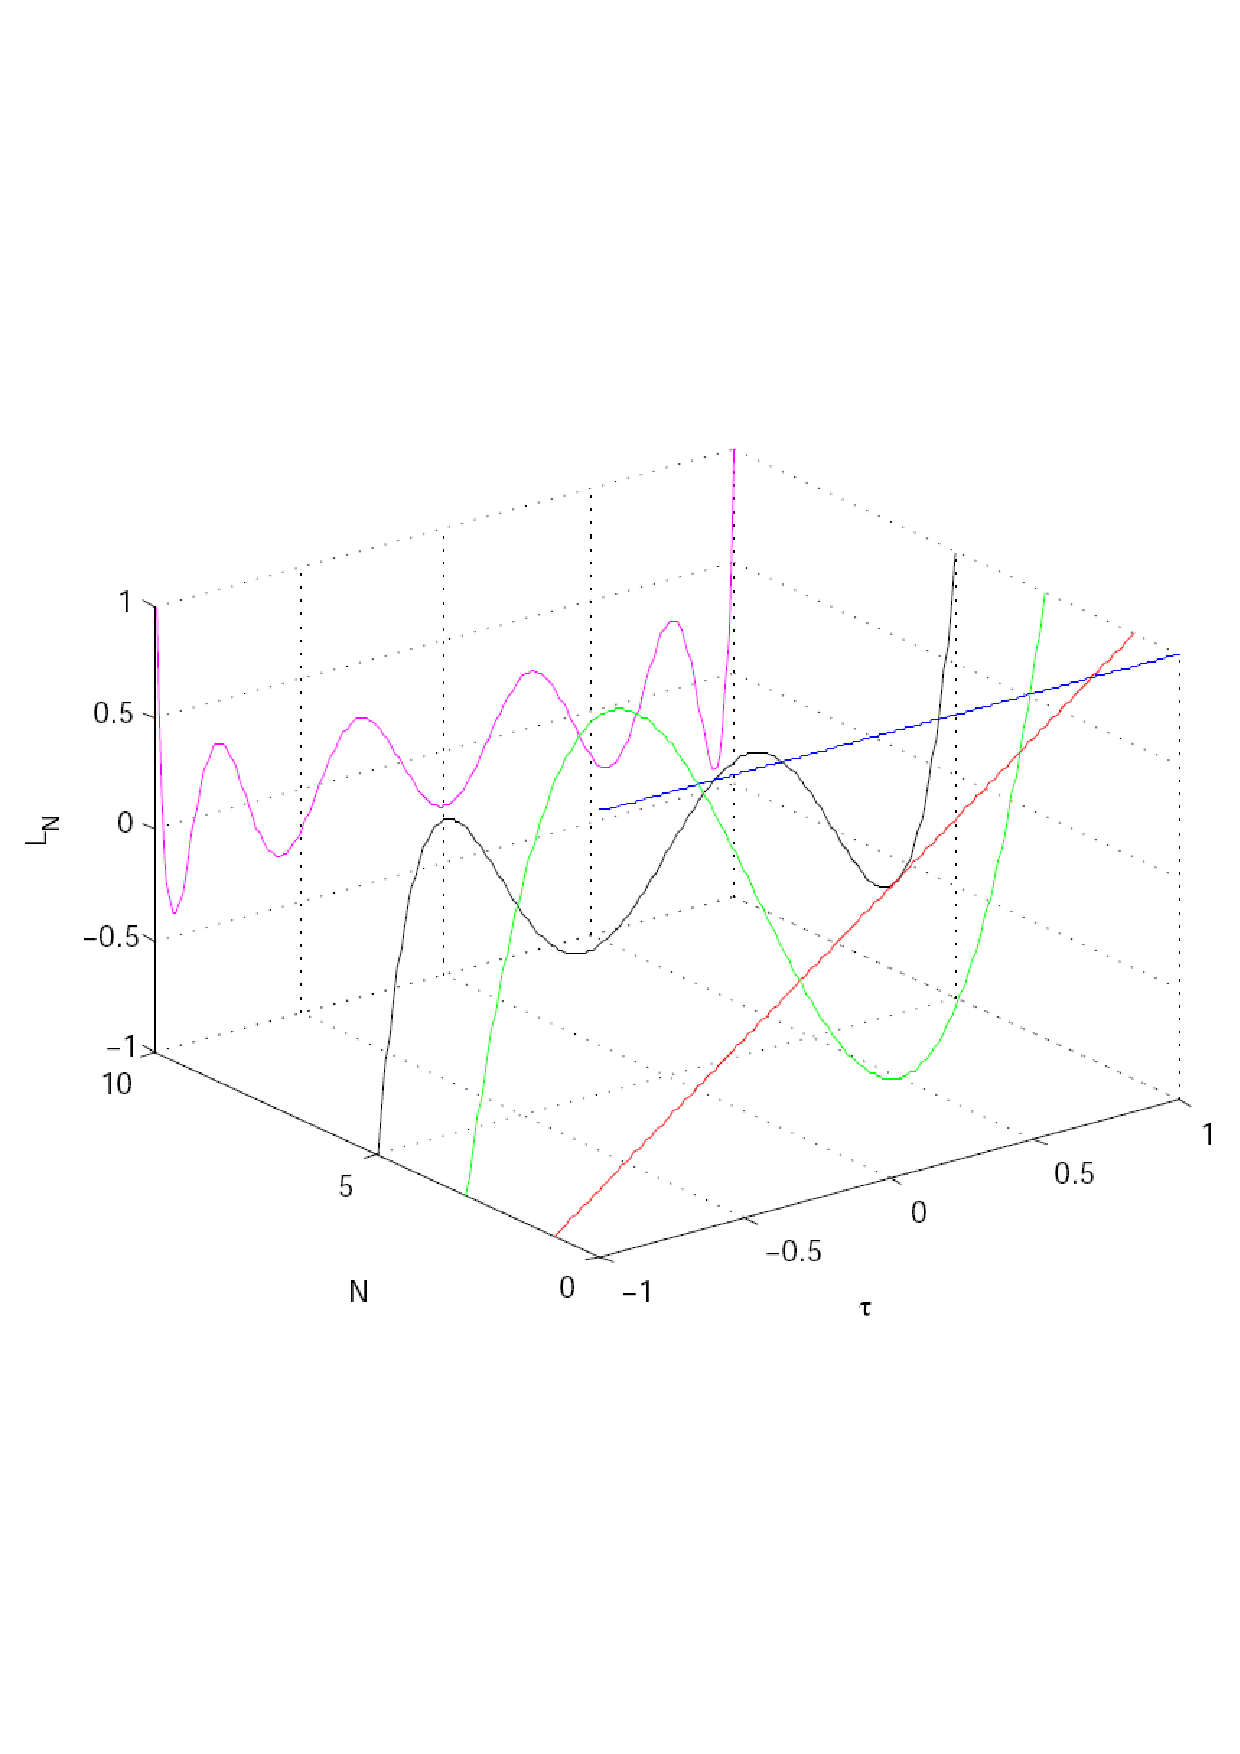
\includegraphics[height=8cm]{legendrepoly.pdf}}
\caption{Illustration of the Legendre polynomials $L_N(\tau)$ for $N = 0,1,2, 4,5, 10$.}
\label{legendrepoly}
\end{figure}



 Let $\tau_k$, $k=0,\ldots,N$ be the Lagrange-Gauss-Lobatto (LGL) nodes, which are defined
 as $\tau_0 = -1$, $\tau_N = 1$, and $\tau_k$, being the roots of $\dot L_N(\tau)$ in the
interval $[-1, 1]$ for $k = 1,2,\ldots, N - 1$. There are no explicit formulas to compute the roots of $\dot L_N(\tau)$, but they can be computed
using known numerical algorithms. For example, for $N=20$, the LGL nodes $\tau_k, k=0,\ldots,20$ are shown
in Figure \ref{fig:lglnodes}. 


\begin{figure}[htbp] 
 \centerline{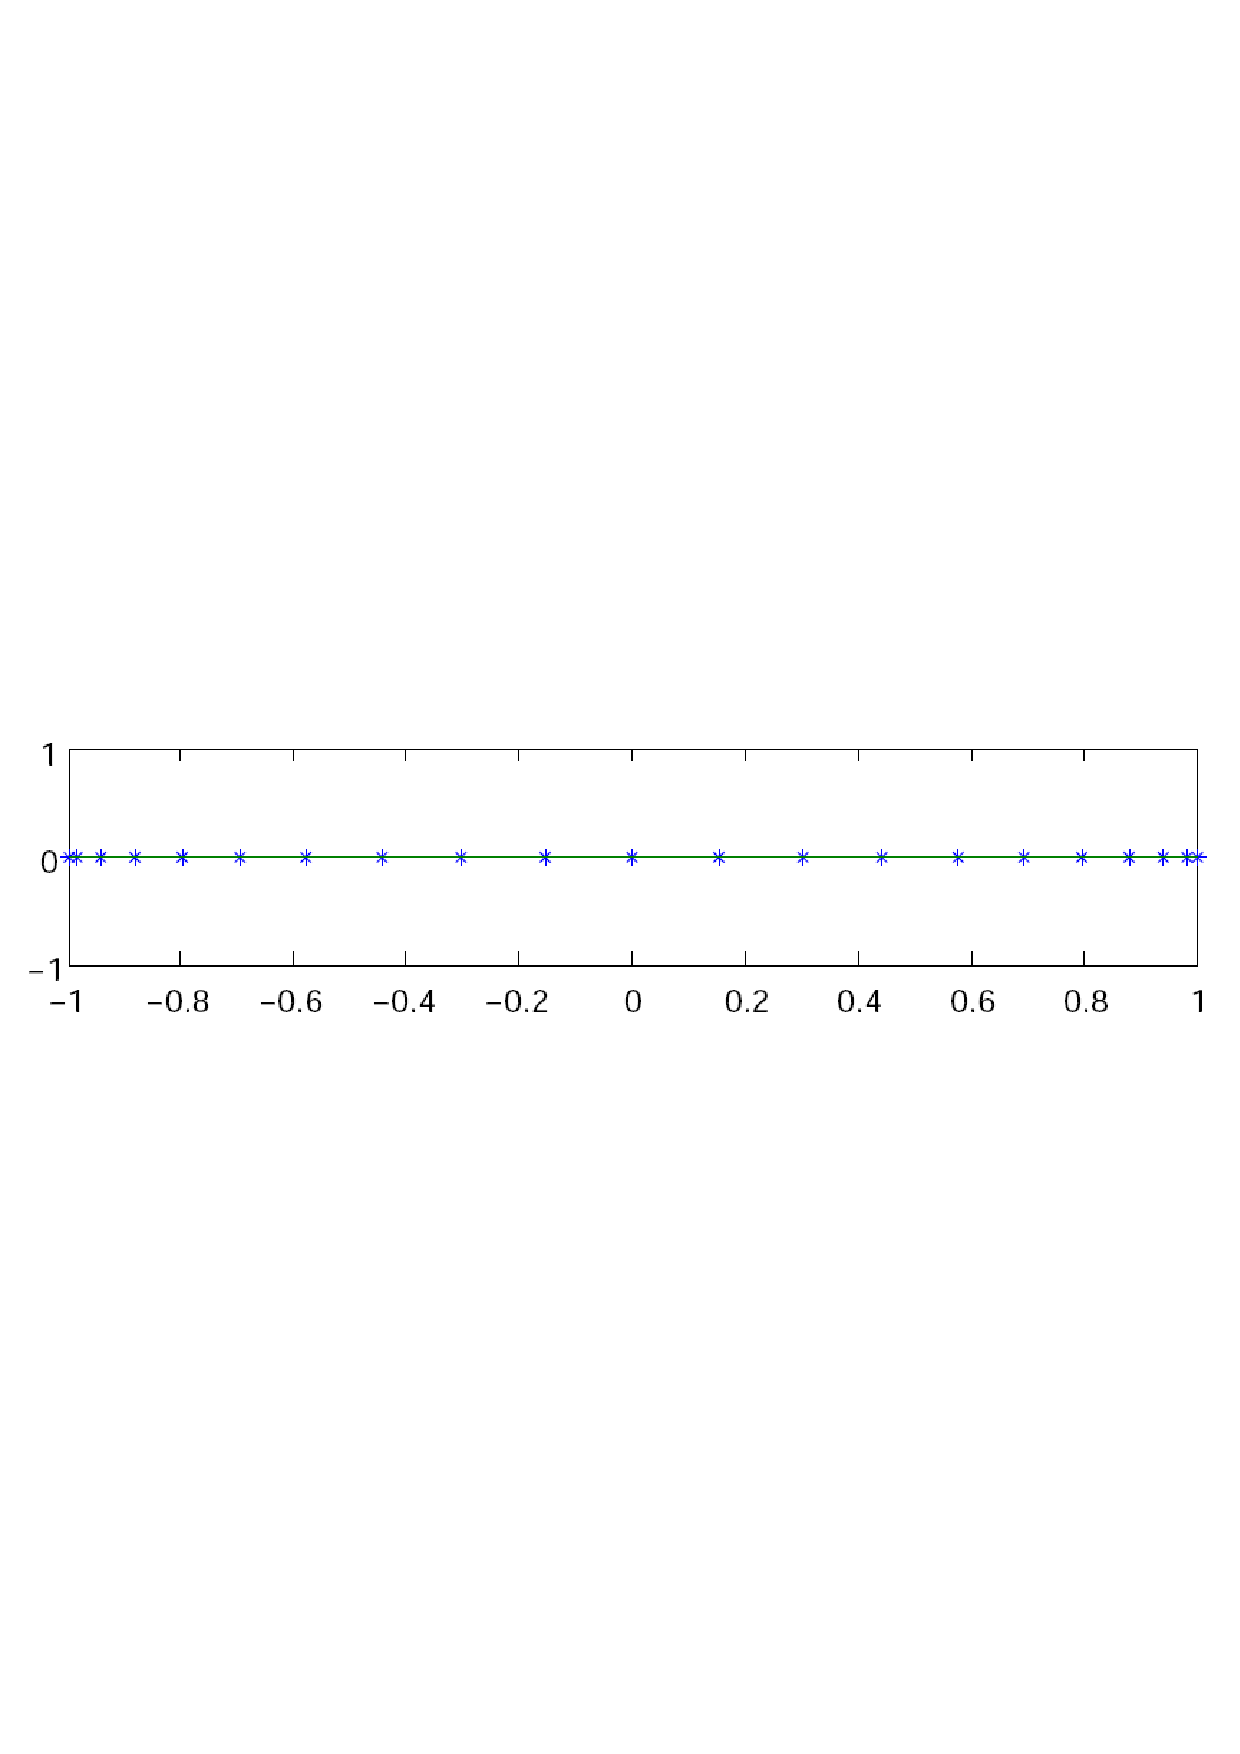
\includegraphics[width=14cm]{lglnodesplot}}
\caption{Illustration of the Legendre Gauss Lobatto (LGL) nodes for $N=20$.}
\label{fig:lglnodes}
\end{figure}



        Note that if $h(\tau)$ is a polynomial of degree $\le 2N-1$, its integral over
$\tau \in [-1,1]$ can be exactly computed as follows:

\begin{equation}
 \int_{-1}^{1} h(\tau) d\tau = \sum\limits_{k=0}^N h(\tau_k) w_k
\end{equation}
where $\tau_k$, $k=0,\ldots,N$ are the LGL nodes and the weights $w_k$ are
given by:
\begin{equation} \label{quad_weights}
  w_k = \frac{2}{N(N+1)} \frac{1}{[L_N(\tau_k)]^2},\,\, k=0,\ldots,N.
\end{equation}

If $L(\tau)$ is a general smooth function, then for a suitable $N$, its  integral over $\tau\in[-1,1]$ can be approximated as follows:
\begin{equation}
 \int_{-1}^{1} L(\tau) d\tau \approx \sum\limits_{k=0}^N L(\tau_k) w_k
\end{equation}

The LGL nodes are selected to yield highly accurate numerical integrals.
For example, consider the definite integral 
\[\int_{-1}^1 e^t \cos(t) dt\]
The exact value of this integral to 7 decimal places is 1.9334214. 
For $N=3$ we have $\tau = [-1, -0.4472, 0.4472, 1]$, $w =[ 0.1667, 0.8333, 0.8333, 0.1667]$,
hence 

\[ \int_{-1}^1 e^t \cos(t) dt \approx w^T h(\tau) = 1.9335 \]
so that the error is $\mathcal{O}(10^{-5})$.
On the other hand, if $N=5$, then the approximate value is 1.9334215, so that the
error is $\mathcal{O}(10^{-7})$.




\subsection{Interpolation and Legendre polynomials}

The Legendre-Gauss-Lobatto quadrature motivates the following expression to approximate the weights
of the expansion (\ref{eq:expansion_coefficients}):
\[
  \hat f_k \approx \tilde f_k = \frac{1}{\gamma_k} \sum\limits_{j=0}^N f(\tau_j) L_k(\tau_j) w_j
\]
where
\[
   \gamma_k = \sum_{j=0}^N L_k^2(\tau_j) w_j
\]
It is simple to prove (see \cite{Hesthaven:07}) that with these weights, function $f : [-1,1]\rightarrow \Re$ 
can be interpolated over the LGL nodes as a discrete expansion using Legendre polynomials:
\begin{equation} \label{eq:Legendre_expansion}
    I_N f(\tau) = \sum\limits_{k=0}^N \tilde f_k L_k(\tau)
\end{equation}
such that
\begin{equation} \label{eq:colloc}
   I_N f(\tau_j) = f(\tau_j)
\end{equation}


Because $I_N f(\tau)$ is an interpolant of $f(\tau)$ at the LGL nodes, and since the interpolating 
polynomial is unique, we may express $I_N f(\tau)$ as a Lagrange interpolating polynomial:
\begin{equation} \label{eq:Lagrange_expansion}
    I_N f(\tau) = \sum\limits_{k=0}^N f(\tau_k) \mathcal{L}_k(\tau)
\end{equation}
so that the expressions (\ref{eq:Legendre_expansion}) and (\ref{eq:Lagrange_expansion}) are mathematically
equivalent. Expression (\ref{eq:Lagrange_expansion}) is computationally advantageous since,
as discussed below, it allows to express the approximate values of the derivatives of the function 
$f$ at the nodes as a matrix multiplication. It is possible to write the Lagrange basis polynomials
$\mathcal{L}_k(\tau)$  as follows \cite{Hesthaven:07}:
\[
  \mathcal{L}_k(\tau) = \frac{1}{N(N+1)L_N(\tau_k)} \frac{(\tau^2-1) \dot L_N(\tau)}{\tau-\tau_k}
\]

The use of polynomial interpolation to approximate a function using the LGL points is known in
the literature as the \textit{Legendre pseudospectral approximation method}. Denote $f^N(\tau) = I_N f(\tau)$. Then,
we have:
\begin{equation} \label{legendre_approx}
    f(\tau) \approx f^N(\tau) = \sum\limits_{k=0}^N f(\tau_k) \mathcal{L}_k(\tau)
\end{equation}


It should be noted that $\mathcal{L}_k(\tau_j)=1$ if $k=j$ and $\mathcal{L}_k(\tau_j)$=0, if $k\ne j$, so that:
\begin{equation} \label{eq:colloc}
f^N(\tau_k) = f(\tau_k)
\end{equation}

Regarding the accuracy and error estimates of the Legendre pseudospectral approximation,
it is well known that for smooth functions $f(\tau)$, the
rate of convergence of $f^N(\tau)$ to $f(\tau)$  at the collocation points is faster
than any power of $1/N$. The convergence of the pseudospectral approximations used
by \psopt has been analysed by Canuto \textit{et al} \cite{Canuto:06}.

Figure \ref{fig:interpolation} shows the degree $N$ interpolation of the function $f(\tau) = 1/(1 + \tau + 15\tau^2 )$ in $(N + 1)$ equispaced
and LGL points for $N = 20$. With increasing $N$, the errors increase
exponentially in the equispaced case (this is known as the Runge phenomenon) 
whereas in the LGL case they decrease exponentially.

%\vspace{-3.0cm}
\begin{figure}[htbp] 
 \centerline{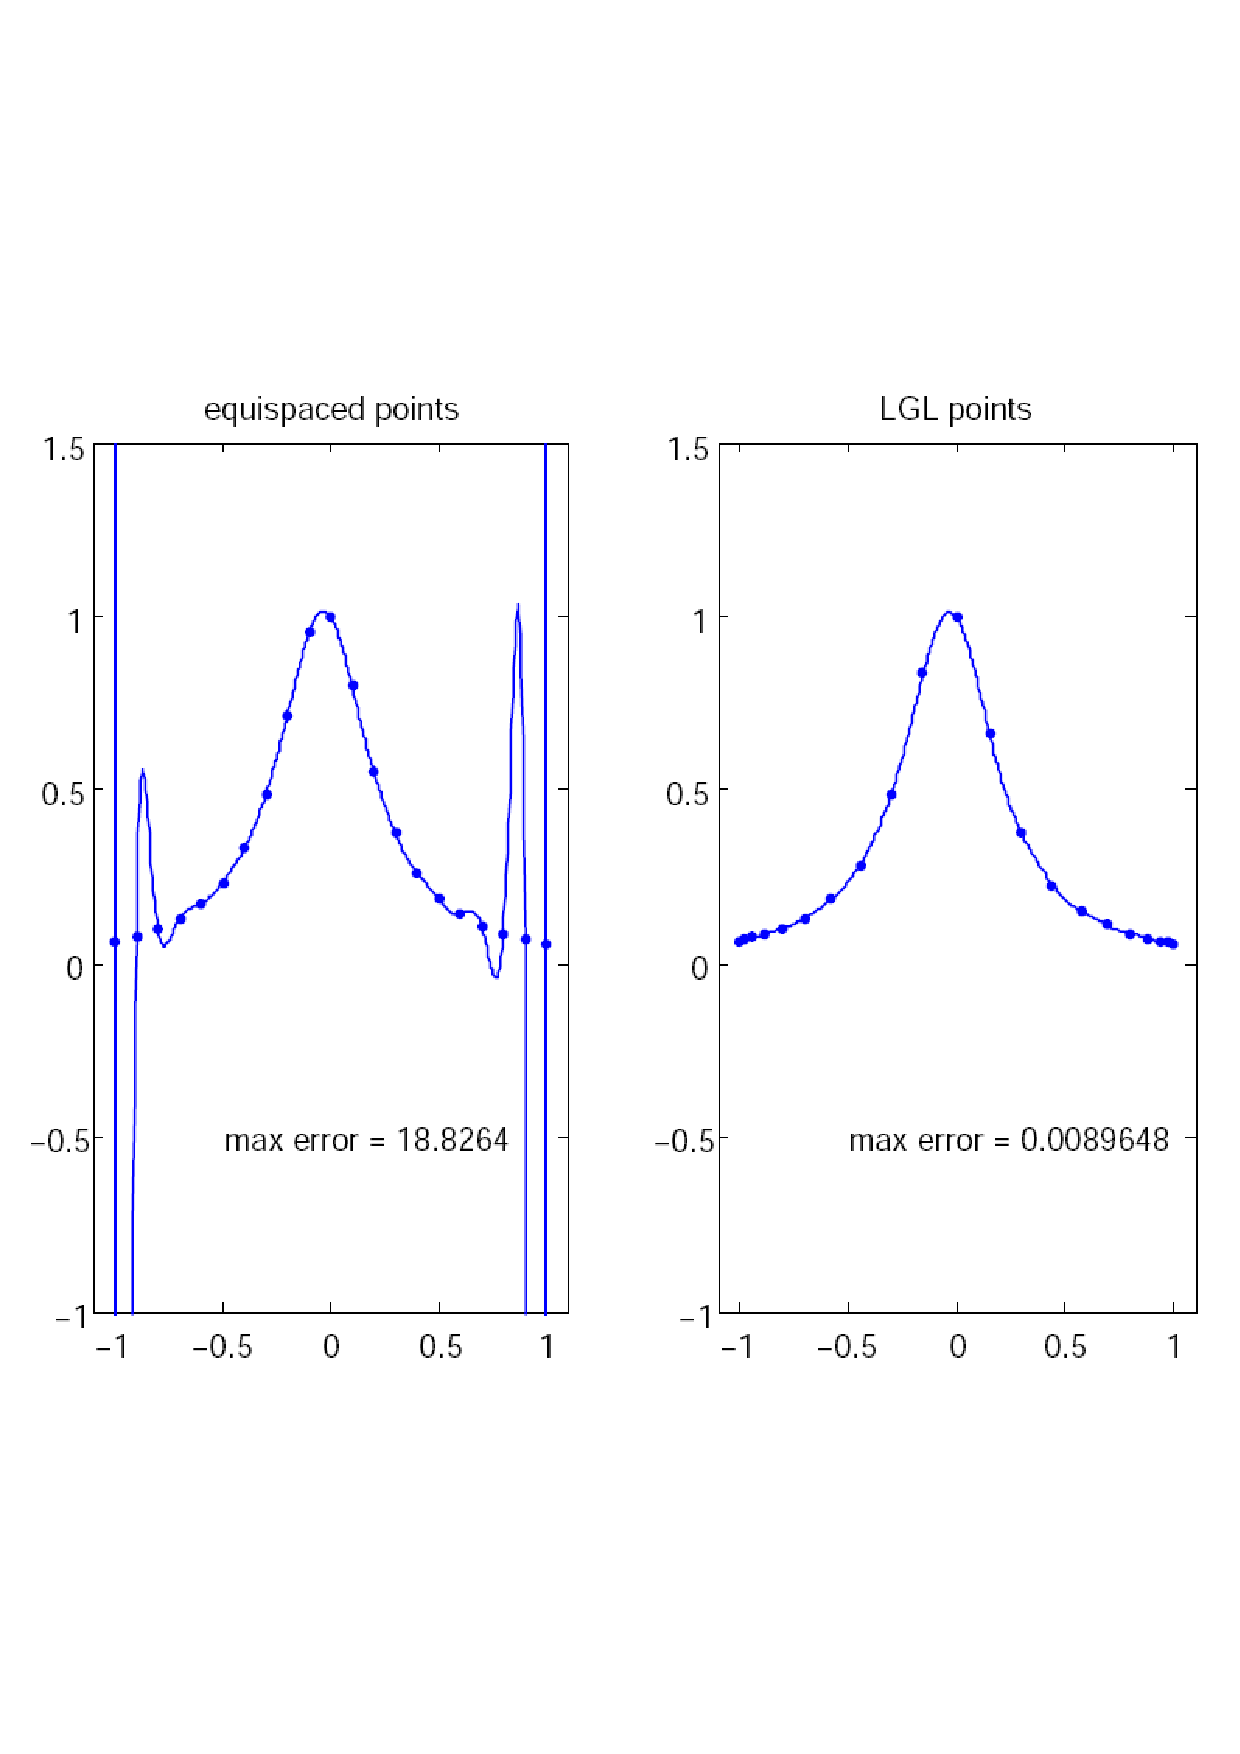
\includegraphics[height=10cm]{interpolation_example}}
\caption{Illustration of polynomial interpolation over equispaced and LGL nodes}.
\label{fig:interpolation}
\end{figure}


%%%%%%%%%%%%%%%%%%%%%%%%%%%%%%%%%%%%%%%%%%%%%%%%%%%%%%%%%%%%%%%%%%%%%%%%%%%%%%%%%%%%%%%%%%%%%%%%%%%
\subsection{Approximate differentiation}

The derivatives of $f^N(\tau)$ in terms of $f(\tau)$ at the LGL points $\tau_k$ can be obtained
by differentiating  Eqn. (\ref{legendre_approx}). The result can be expressed as a matrix
multiplication, such that:

\[ 
  \dot f(\tau_k) \approx \dot f^N(\tau_k) = \sum \limits_{i=0}^N D_{ki} f(\tau_i)
\]
where 
\begin{equation} \label{diff_matrix}
   D_{ki} = \left\{ \begin{matrix} -\frac{L_N(\tau_k)}{L_N(\tau_i)} \frac{1}{\tau_k-\tau_i} & \mathrm{if} \, k\ne i \\
                    N(N+1)/{4} & \mathrm{if} \, k=i=0 \\
                     -N(N+1)/{4} & \mathrm{if} \, k=i=N \\
                        0    & \mathrm{otherwise}  \end{matrix}  \right.
\end{equation}
which is known as the differentiation matrix.






For example, this is the Legendre differentiation matrix for $N=5$.

\[
D=
\begin{bmatrix}
   7.5000 & -10.1414  &  4.0362 &  -2.2447&    1.3499&   -0.5000 \\
    1.7864&         0&   -2.5234&    1.1528&   -0.6535&    0.2378 \\
   -0.4850&    1.7213&         0&   -1.7530&    0.7864&   -0.2697  \\
    0.2697&   -0.7864&    1.7530&         0&   -1.7213&    0.4850 \\
   -0.2378&    0.6535&   -1.1528&    2.5234&         0&   -1.7864 \\
    0.5000&   -1.3499&    2.2447&   -4.0362&   10.1414&   -7.5000 \\
\end{bmatrix}
\]





Figure \ref{fig:diff_example}   shows the  Legendre differentiation of $f(t)= \sin(5t^2)$ for $N=20$ and $N=30$. Note the vertical
scales in the error curves. Figure \ref{fig:diff_error} shows the maximum error in the Legendre differentiation of $f(t)=\sin(5t^2)$ as a function of $N$. Notice
that the error initially decreases
very rapidly until such high precision is achieved (accuracy in the order of $10^{-12}$) that round off errors due to
the finite precision of the computer prevent any further reductions. This phenomenon is known as \textit{spectral accuracy}.

%\vspace{-4.0cm}
\begin{figure}[htbp]
 \centerline{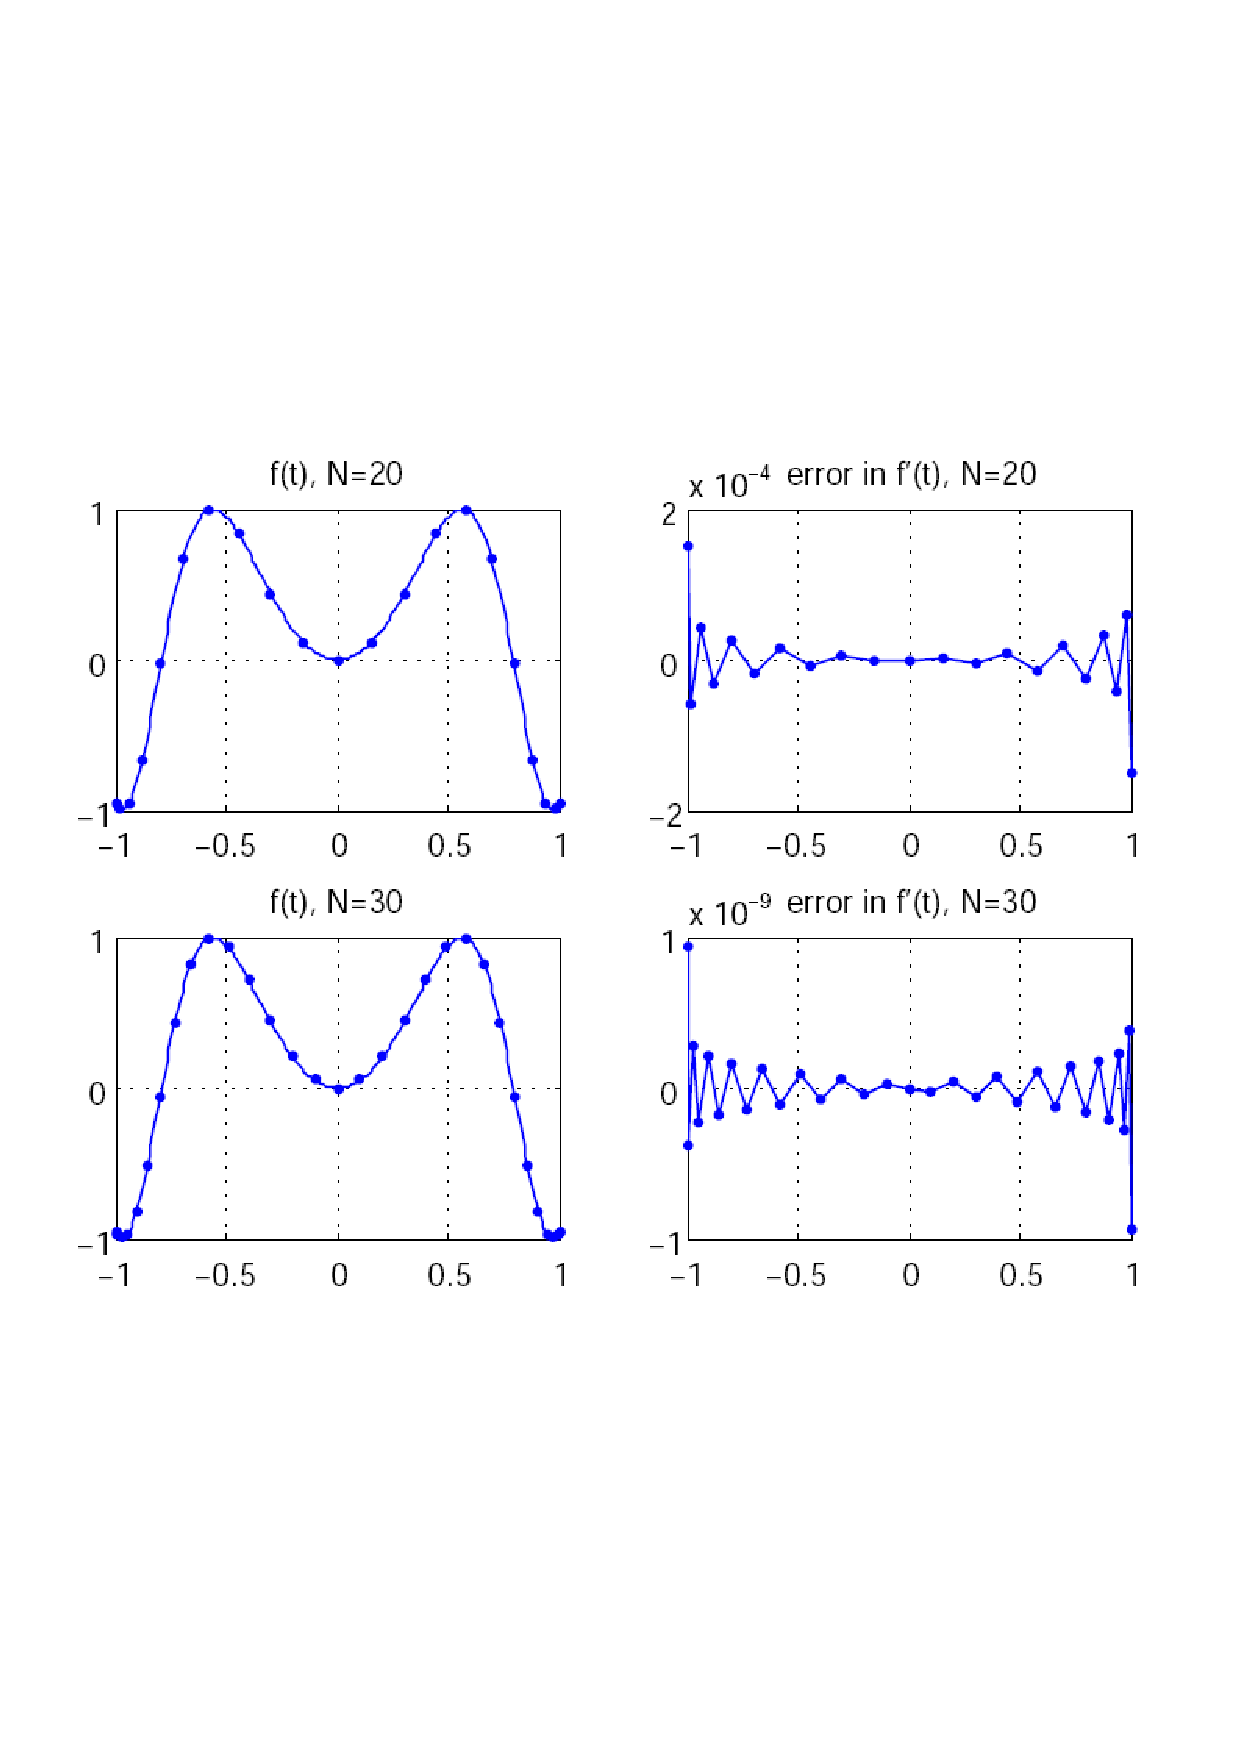
\includegraphics[height=10cm]{derivatives_example}}
\caption{Legendre differentiation of $f(t)=\sin(5t^2)$ for $N=20$ and $N=30$.}
 \label{fig:diff_example} 
\end{figure}

\begin{figure}[htbp] 
 \centerline{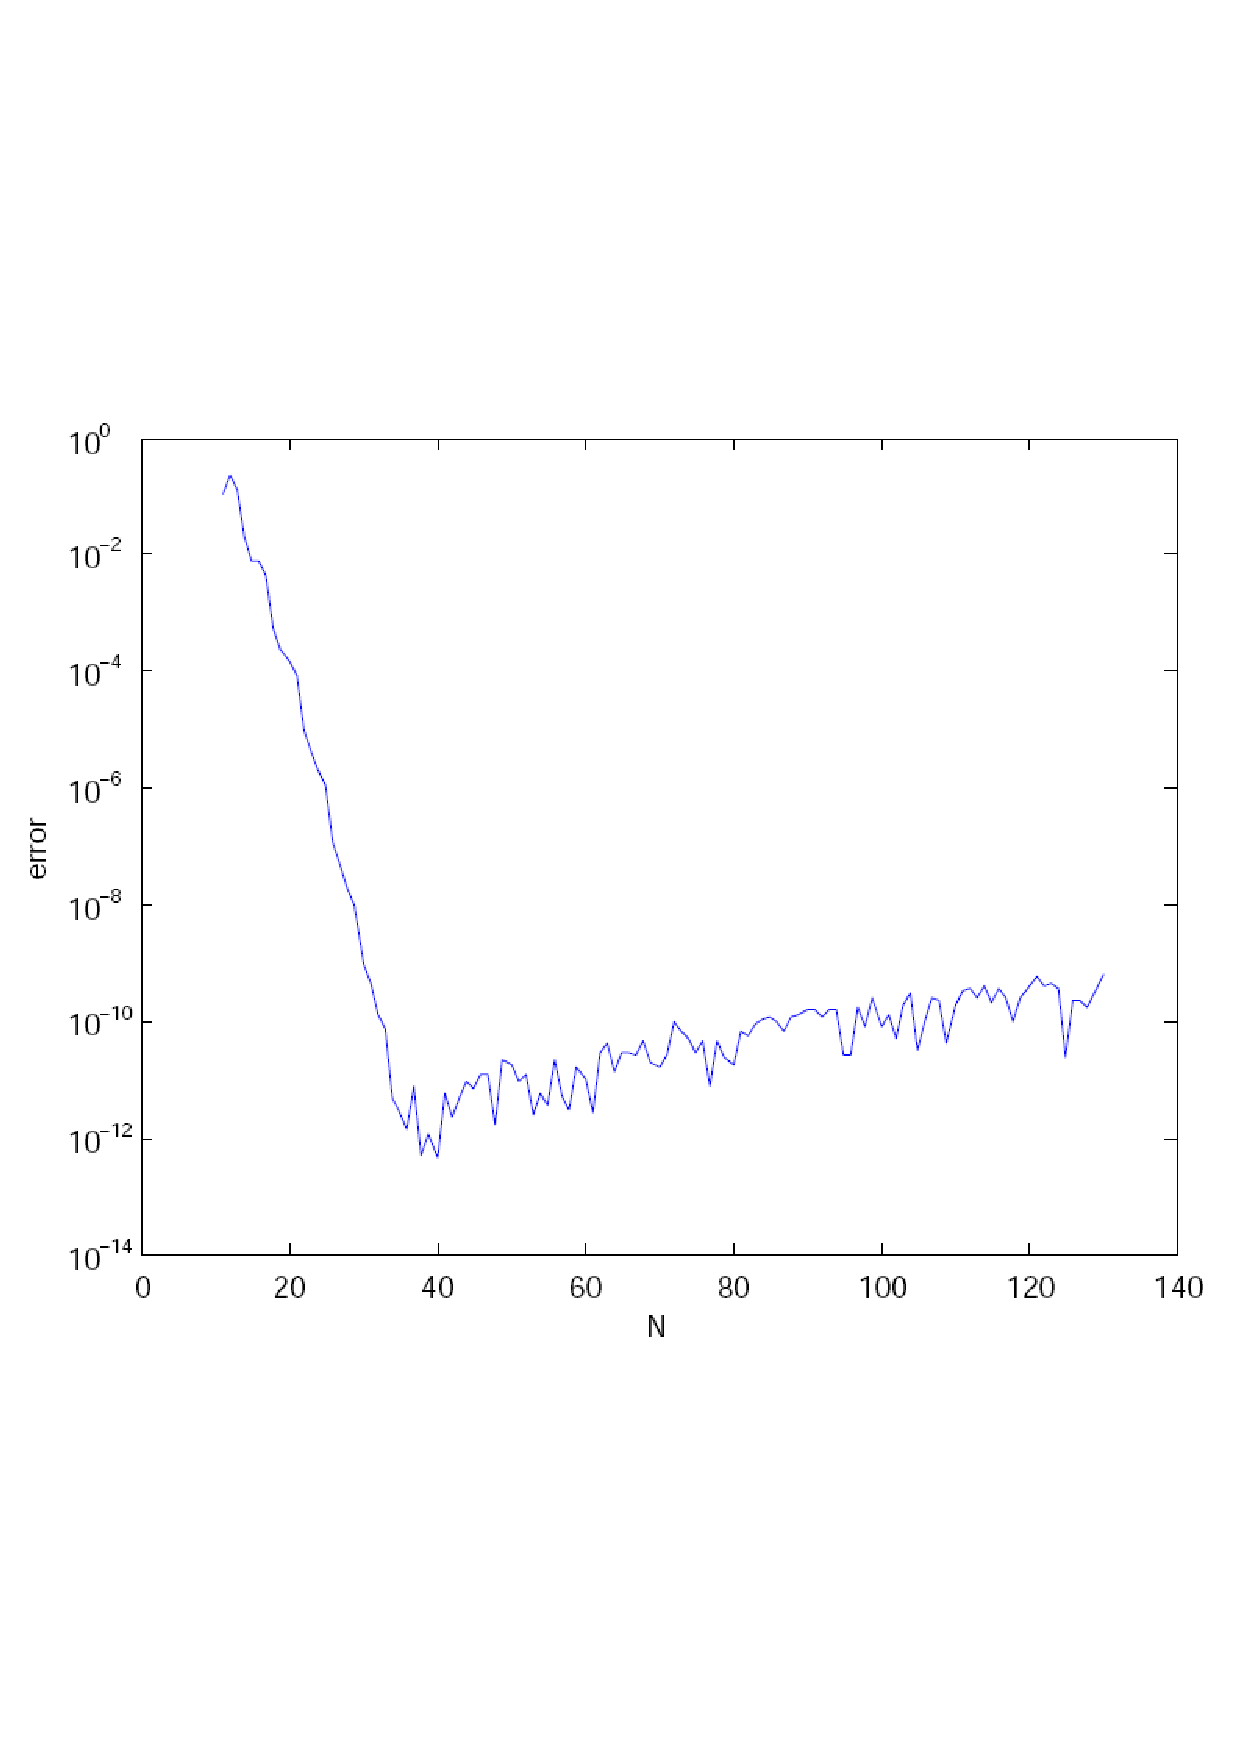
\includegraphics[height=10cm]{derivatives_error}}
\caption{Maximum error in the Legendre differentiation of $f(t)=\sin(5t^2)$ as a function of $N$.}
\label{fig:diff_error} 
\end{figure}










%**************************************************************



\subsection{Approximating a continuous function using Chebyshev polynomials}


\psopt also has facilities for pseudospectral function approximation using Chebyshev polynomials. 
Let $T_N(\tau)$ denote the Chebyshev polynomial of order $N$,
which may be generated from:
\begin{equation}
  T_N(\tau) = \cos( N \cos^{-1} (\tau)  )
\end{equation}
 Let $\tau_k$, $k=0,\ldots,N$ be the Chebyshev-Gauss-Lobatto (CGL) nodes in the interval $[-1,1]$, 
which are defined as $\tau_{k} = -\cos(\pi k /N)$ for $k = 0,1,\ldots, N$.

Given any
real-valued function $f(\tau): [-1,1]\rightarrow \Re$, it can be approximated by the Chebyshev
pseudospectral method:
\begin{equation} \label{chebyshev_approx}
  f(\tau) \approx f^{N}(\tau) = \sum_{k=0}^{N} f(\tau_k) \varphi_k(\tau)
\end{equation}
where the Lagrange interpolating polynomial $\varphi_k(\tau)$ is defined by:

\begin{equation}
  \varphi_k(\tau) = \frac{(-1)^{k+1}}{N^2 \bar c_k} \frac{(1-\tau^2) \dot T_N(\tau)}{\tau-\tau_k}
\end{equation}
where
\begin{equation}
   \bar c_k = \left\{ \begin{array}{ll} 2 & k=0,N \\ 1 & 1\le k\le N-1 \end{array} \right.
\end{equation}

It should be noted that $\varphi_k(\tau_j)=1$ if $k=j$ and $\varphi_k(\tau_j)$=0, if $k\ne j$, so that:
\begin{equation} \label{eq:colloc_chev}
f^N(\tau_k) = f(\tau_k)
\end{equation}




\subsection{Differentiation with Chebyshev polynomials}

The derivatives of $f^N(\tau)$ in terms of $f(\tau)$ at the CGL points $\tau_k$ can be obtained
by differentiating (\ref{chebyshev_approx}). The result can be expressed as a matrix
multiplication, such that:

\begin{equation} \label{fdot_approx_cheb}
  \dot f(\tau_k) \approx \dot F^N(\tau_k) = \sum \limits_{i=0}^N D_{ki} f(\tau_i)
\end{equation}
where 
\begin{equation} \label{eq:diff_mat_cheb}
   D_{ki} = \left\{ \begin{matrix} \frac{\bar c_k }{2 \bar c_i } \frac{(-1)^{k+i}}{\sin[(k+i)\pi/2N] \sin[(k-i)\pi/2N]} & \mathrm{if} \, k\ne i \\
                    \frac{\tau_k}{2\sin^2[k\pi/N]} & \mathrm{if} \, i\le k=i \le N-1 \\
                    -\frac{2N^2+1}{6} & \mathrm{if} \, k=i=0 \\
                       \frac{2N^2+1}{6}    & \mathrm{if} \,\, k=i=N  \end{matrix}  \right.
\end{equation}
which is known as the differentiation matrix.




\subsection{Numerical quadrature with the Chebyshev-Gauss-Lobatto method}


Note that if $h(\tau)$ is a polynomial of degree $\le 2N-1$, its weighted integral over
$\tau \in [-1,1]$ can be exactly computed as follows:

\begin{equation}
 \int_{-1}^{1} g(\tau) h(\tau) d\tau = \sum\limits_{k=0}^N h(\tau_k) w_k
\end{equation}
where $\tau_k$, $k=0,\ldots,N$ are the CGL nodes, d the weights $w_k$ are
given by:
\begin{equation} \label{cheb_quad_weights}
  w_k = \left\{ \begin{array}{ll} \frac{\pi}{2N}, & k=0,\ldots,N.\\
                                   \frac{\pi}{N},  & k=1,\ldots,N-1
                 \end{array} \right.
\end{equation}
and $g(\tau)$ is a weighting function given by:
\begin{equation}
    g(\tau) = \frac{1}{\sqrt{1-\tau^2}}
\end{equation}


If $L(\tau)$ is a general smooth function, then for a suitable $N$, its weighted  integral over $\tau\in[-1,1]$ can be approximated as follows:
\begin{equation}
 \int_{-1}^{1} g(\tau) L(\tau) d\tau \approx \sum\limits_{k=0}^N L(\tau_k) w_k
\end{equation}


\subsection{Differentiation with reduced round-off errors}

The following differentiation matrix, which offers reduced round-off errors \cite{Canuto:06}, is employed optionally by \psopt.
It can be  used both with Legrendre and Chebyshed points. 

\begin{equation} \label{diff_mat_reduced_roundoff}
 D_{jl} = \left \{  \begin{array}{ll} - \frac{\delta_l}{\delta_j} \frac{(-1)^{j+l}}{\tau_j-\tau_l} & j\ne l\\
                                        \sum\limits_{i=0,i\ne j}^N \frac{\delta_i}{\delta_j}\frac{(-1)^{i+j}}{\tau_j-\tau_i} &  j=l
                   \end{array} \right. 
\end{equation}


\section{The pseudospectral discretizations used in \psopt}

To illustrate the pseudospectral discretizations employed in \psopt, consider the following single phase continuous optimal control problem:


\subsection*{Problem $\mathcal{P}_2$} Find the control trajectories, $u(t), t\in [t_0, t_f]$, state trajectories $x(t), t\in [t_0, t_f]$,  static parameters $p$, and 
times $t_0, t_f$, to minimise the following performance index:
\[
   J =  \varphi[ x(t_0), x(t_f), p, t_0, t_f ] + \int_{t_0}^{t_f} L[x(t),u(t),p, t] dt 
\]

\noindent subject to the differential constraints:
\[
 \dot x(t) = f[ x(t),u(t), p, t ],  \,t\in[t_0,t_f],
\]
the path constraints
\[
 h_L \le h[ x(t),u(t), p, t ] \le h_U,  \,t\in[t_0,t_f]
\]
the event constraints:
\[
 e_L \le e[ x(t_0),u(t_0),x(t_f),u(t_f), p, t_0, t_f ] \le e_U, 
\]
the bound constraints on states and controls:
\[
    u_L \le u(t) \le u_U, \, t\in[t_0,t_f], 
\]
\[
    x_L \le x(t) \le x_U, \, t\in[t_0,t_f], 
\]
and the constraints:
\[
    \underline{t}_0 \le t_0 \le \bar{t}_0, 
\]
\[
    \underline{t}_f \le t_f \le \bar{t}_f, 
\]
\[
    t_f - t_0 \ge 0, 
\]

\noindent where
\begin{equation}
\begin{aligned}
  u&: [t_0, t_f] \rightarrow \RE^{n_u} \\
  x&: [t_0, t_f] \rightarrow \RE^{n_x} \\
  p &\in \RE^{n_p} \\
  \varphi&: \RE^{n_x} \times \RE^{n_x} \times \RE^{n_p} \times \RE \times \RE \rightarrow \RE \\
  L&: \RE^{n_x} \times \RE^{n_u} \times \RE^{n_p} \times [t_0,t_f] \rightarrow \RE  \\
  f&: \RE^{n_x} \times \RE^{n_u} \times \RE^{n_p} \times [t_0,t_f] \rightarrow \RE^{n_x}  \\
  h&: \RE^{n_x} \times \RE^{n_u} \times \RE^{n_p} \times [t_0,t_f] \rightarrow \RE^{n_h}  \\
  e&: \RE^{n_x} \times \RE^{n_u} \times \RE^{n_x} \times \RE^{n_u} \times \Re^{n_p} \times \RE \times \RE  \rightarrow \RE^{n_e}  
\end{aligned}
\end{equation}



By introducing the transformation:
\[
  \tau \leftarrow \frac{2}{t_f-t_0} t - \frac{t_f+t_0}{t_f-t_0},
\]
it is possible to write problem $\mathcal{P}_3$ using a new independent variable  $\tau$ in the interval $[-1,1]$, as follows:

\subsection*{Problem $\mathcal{P}_3$} Find the control trajectories, $u(\tau), \tau \in [-1, 1]$, state trajectories $x(\tau), \tau \in [-1, 1]$,  and 
times $t_0, t_f$, to minimise the following performance index:
\[
   J =  \varphi[ x(-1), x(1), p, t_0, t_f ] +\frac{t_f-t_0}{2} \int_{-1}^{1} L[x(t),u(t),p,t] d\tau
\]

\noindent subject to the differential constraints:
\[
 \dot x(\tau) = \frac{t_f-t_0}{2} f[ x(\tau),u(\tau),p,\tau ],  \,\tau \in[-1,1],
\]
the path constraints
\[
 h_L \le h[ x(\tau),u(\tau),p,\tau ] \le h_U,  \,\tau\in[-1,1]
\]
the event constraints:
\[
 e_L \le e[ x(-1),u(-1),x(1),u(1),p,t_0, t_f ] \le e_U, 
\]
the bound constraints on controls and states:
\[
    u_L \le u(\tau) \le u_U, \, \tau \in[-1,1], 
\]
\[
    x_L \le x(\tau) \le x_U, \, \tau \in[-1,1], 
\]
and the constraints:
\[
    \underline{t}_0 \le t_0 \le \bar{t}_0, 
\]
\[
    \underline{t}_f \le t_f \le \bar{t}_f, 
\]
\[
    t_f - t_0 \ge 0, 
\]


The description below refers to  the Legendre pseudospectral approximation method. The procedure employed with the Chebyshev approximation method
is very similar. In the Legendre pseudospectral approximation of problem $\mathcal{P}_3$, the state $x(\tau)$, $\tau \in [-1,1]$ is approximated
by the $N$-order Lagrange polynomial $x^N(\tau)$ based on interpolation at the Legendre-Gauss-Lobatto (LGL) quadrature
nodes, so that:
\begin{equation}
  x(\tau) \approx x^{N}(\tau) = \sum_{k=0}^{N} x(\tau_k) \phi_k(\tau)
\end{equation}

Moreover, the control $u(\tau)$, $\tau \in [-1,1]$ is similarly approximated using an interpolating polynomial:
\begin{equation}
  u(\tau) \approx u^{N}(\tau) = \sum_{k=0}^{N} u(\tau_k) \phi_k(\tau)
\end{equation}
Note that, from (\ref{eq:colloc}), $x^N(\tau_k)=x(\tau_k)$ and $u^N(\tau_k)=u(\tau_k)$.
The derivative of the state vector is approximated as follows:

\begin{equation} \label{eq:xdot_approx}
\dot x(\tau_k) \approx \dot x^N(\tau_k) = \sum \limits_{i=0}^N D_{ki} x^N(\tau_i), \, i=0,\ldots N
\end{equation}
where  $D$ is the $(N+1)\times(N+1)$ the differentiation matrix given by (\ref{eq:diff_mat}).

Define the following $n_u \times (N+1)$ matrix  to store the trajectories of
the controls at the LGL nodes:

\begin{equation}
   U^N = \begin{bmatrix} 
           u_1(\tau_0)& u_1(\tau_1)& \ldots& u_{1}(\tau_N) \\
           u_2(\tau_0)& u_2(\tau_1)& \ldots& u_{2}(\tau_N) \\
           \vdots &   \vdots &  \ddots&, \vdots \\
           u_{n_u}(\tau_0)& u_{n_u}(\tau_1)& \ldots& u_{n_u}(\tau_N) \\
         \end{bmatrix}
\end{equation}


Define the following $n_x \times (N+1) $ matrices to store, respectively, the trajectories of
the states and their derivatives at the LGL nodes:

\begin{equation}
   X^N = \begin{bmatrix} 
           x_1(\tau_0)& x_1(\tau_1)& \ldots& x_{1}(\tau_N) \\
           x_2(\tau_0)& x_2(\tau_1)& \ldots& x_{2}(\tau_N) \\
           \vdots &   \vdots &  \ddots&, \vdots \\
           x_{n_x}(\tau_0)& x_{n_x}(\tau_1)& \ldots& x_{n_x}(\tau_N) \\
         \end{bmatrix}
\end{equation}

and

\begin{equation}
   \dot X^N = \begin{bmatrix} 
          \dot x_1(\tau_0)& \dot x_1(\tau_1)& \ldots& \dot x_{1}(\tau_N) \\
          \dot  x_2(\tau_0)& \dot  x_2(\tau_1)& \ldots&\dot  x_{2}(\tau_N) \\
           \vdots &   \vdots &  \ddots&, \vdots \\
          \dot  x_{n_x}(\tau_0)& \dot x_{n_x}(\tau_1)& \ldots& \dot x_{n_x}(\tau_N) \\
         \end{bmatrix}
\end{equation}


From (\ref{eq:xdot_approx}), $X^N$ and $\dot X_N$ are related as follows:

\begin{equation}
    \dot X^N = X^N D^T
\end{equation}

Now, form the following $n_x \times (N+1) $ matrix with the right hand side of the differential constraints evaluated
at the LGL nodes:

\begin{equation}
    F^N = \frac{t_0-t_f}{2} \begin{bmatrix} 
           f_1(x^N(\tau_0),u^N(\tau_0),p,\tau_0)&  \ldots& f_{1}(x^N(\tau_N),u^N(\tau_N),p,\tau_N) \\
           f_2(x^N(\tau_0),u^N(\tau_0),p,\tau_0)&  \ldots& f_{2}(x^N(\tau_N),u^N(\tau_N),p,\tau_N)\\
           \vdots    &  \ddots& \vdots \\
           f_{n_x}(x^N(\tau_0),u^N(\tau_0),p,\tau_0)&  \ldots& f_{n_x}(x^N(\tau_N),u^N(\tau_N),p,\tau_N)
         \end{bmatrix}
\end{equation}

Now, define the differential defects at the collocation points as the $n_x\times (N+1)$ matrix:
\begin{equation} \label{differential_defects}
   \zeta^N = \dot X^N - F^N = X^N D^T - F^N
\end{equation}

Define the matrix of path constraint function values evaluated at the LGL nodes:
\begin{equation}
    H^N = \begin{bmatrix} 
           h_1(x^N(\tau_0),u^N(\tau_0),p,\tau_0)&  \ldots& h_{1}(x^N(\tau_N),p,u^N(\tau_N),\tau_N) \\
           h_2(x^N(\tau_0),u^N(\tau_0),p,\tau_0)&  \ldots& h_{2}(x^N(\tau_N),u^N(\tau_N),p,\tau_N)\\
           \vdots  &  \ddots& \vdots \\
           h_{n_h}(x^N(\tau_0),u^N(\tau_0),p,\tau_0)&  \ldots& h_{n_h}(x^N(\tau_N),u^N(\tau_N),p,\tau_N)
         \end{bmatrix}
\end{equation}

The objective function of $\mathcal{P}_3$ is approximated as follows:
\begin{equation}
\begin{aligned}
   J &=  \varphi[ x(-1), x(1), p, t_0, t_f ] + \frac{t_f-t_0}{2} \int_{-1}^{1} L[x(\tau),u(\tau),p, \tau] d\tau \\
     &\approx \varphi[ x^N(-1), x^N(1), p, t_0, t_f ] + \frac{t_f-t_0}{2}\sum\limits_{k=0}^N L[ x^N(\tau_k), u^N(\tau_k),p,\tau_k] w_k
\end{aligned}   
\end{equation}
where the weights $w_k$ are defined in (\ref{quad_weights}).

We are now ready to express problem $\mathcal{P}_3$ as a nonlinear programming problem, as follows.

\subsection*{Problem $\mathcal{P}_4$}
\begin{equation}
   \min_y  F(y)
\end{equation}
subject to:
\begin{equation}
 \begin{aligned}
    G_l \le &G(y) \le G_u \\
    y_l \le &y  \le y_u
 \end{aligned}
\end{equation}

The decision vector $y$, which has dimension $n_y=(n_u(N+1)+n_x(N+1)+n_p+2)$, is constructed
as follows:

\begin{equation} \label{single_phase_dv}
   y = \begin{bmatrix}
          \mathrm{vec}(U^N) \\
          \mathrm{vec}(X^N) \\
          p        \\
          t_0      \\
          t_f     
       \end{bmatrix}
\end{equation}

The objective function is:
\begin{equation}
 F(y) = \varphi[ x^N(-1), x^N(1), p, t_0, t_f ] + \frac{t_f-t_0}{2}\sum\limits_{k=0}^N L[ x^N(\tau_k), u^N(\tau_k),p,\tau_k] w_k
\end{equation}
while the constraint function $G(y)$, which is of dimension $n_g=n_x(N+1)+n_h(N+1)+n_e+1$, is given by:
\begin{equation}
         G(y) = \begin{bmatrix}
         \mathrm{vec}(\zeta^N) \\
         \mathrm{vec}(H^N) \\
         e[ x^N(-1),u^N(-1),x^N(1),u^N(1),p,t_0, t_f ]  \\
         t_f - t_0
       \end{bmatrix}, 
\end{equation}
The constraint bounds are given by:
\begin{equation}
G_l = \begin{bmatrix} \mathbf{0}_{n_x (N+1)} \\ \mathrm{stack}(h_L,N+1) \\ e_L \\ (\underline{t}_0-\overline{t}_f) \end{bmatrix}, \,\, G_u
\begin{bmatrix} \mathbf{0}_{n_x (N+1)} \\ \mathrm{stack}(h_U,N+1) \\ e_U \\ 0 \end{bmatrix},
\end{equation}
and the bounds on the decision vector are given by:
\begin{equation}
y_l = \begin{bmatrix} \mathrm{stack}(u_l,N+1) \\ \mathrm{stack}(x_L,N+1) \\ p_L \\ \underline{t}_0 \\ \underline{t}_f \end{bmatrix}, \,\, y_u
\begin{bmatrix}\mathrm{stack}(u_U,N+1) \\ \mathrm{stack}(x_U,N+1) \\ p_U \\ \overline{t}_0 \\ \overline{t}_f \end{bmatrix}, 
\end{equation}
where $\mathrm{vec}(A)$ forms a $nm$-column vector by vertically stacking the columns of the $n\times m$ matrix $A$, and $\mathrm{stack}(x,n)$
creates a $mn$-column vector by stacking $n$ copies of column $m$-vector $x$.


\subsection{Costate estimates} \label{sec:costates}

\subsubsection{Legendre approximation method} \label{sssec:legendre}

\psopt implements the following approximation for the costates $\lambda(\tau) \in \Re^{n_x}, \tau \in [-1,1]$ associated with $\mathcal{P}_3$ \cite{Fahroo:02}:

\begin{equation} \label{eq:costate_legendre}
  \lambda(\tau) \approx \lambda^{N}(\tau) = \sum_{k=0}^{N} \lambda(\tau_k) \phi_k(\tau), \tau \in [-1,1]
\end{equation}
The costate values at the LGL nodes are given by:
\begin{equation}
   \lambda(\tau_k)  = \frac{ \tilde \lambda_k }{ w_k}, \, \, k=0,\ldots N
\end{equation}
where $w_k$ are the weights given by (\ref{quad_weights}), and $\tilde \lambda_k \in \Re^{n_x}$, $k=0,\ldots,N$ are the KKTs multiplier associated with the collocation constraints $\mathrm{vec}(\zeta^N) = 0$. The KKT multipliers can normally be obtained from the NLP solver, which allows \psopt to return estimates of the costate trajectories at the LGL nodes.

It is known from the literature \cite{Fahroo:02} that the costate estimates in the Legendre discretization method sometimes oscillate around the true
values. To mitigate this, the estimates are smoothed by taking a weighted average for the estimats at $k$ using the costate estimates at $k-1$, $k$ and $k+1$
obtained from  (\ref{eq:costate_legendre}).

\subsubsection{Chebyshev approximation method}

\psopt implements the following approximation for the costates $\lambda(\tau) \in \Re^{n_x}, \tau \in (-1,1)$ associated with $\mathcal{P}_3$ 
at the CGL nodes \cite{Pietz:03}:
\begin{equation} \label{lambda_approx_cheb}
   \lambda(\tau_k)  = \frac{ \tilde \lambda_k }{\sqrt{1-\tau_k^2} w_k}, \, \, k=0,\ldots N-1
\end{equation}
where $w_k$ are the weights given by (\ref{cheb_quad_weights}), and $\tilde \lambda_k \in \Re^{n_x}$, $k=0,\ldots,N$ are the KKTs multiplier associated with the collocation constraints $\mathrm{vec}(\zeta^N) = 0$. Since (\ref{lambda_approx_cheb}) is singular for $\tau_0=-1$ and $\tau_N=1$, the estimates of the co-states at $\tau=\pm 1$ are found using linear extrapolation.
The costate estimates are also smoothed as described in \ref{sssec:legendre}

\subsection{Discretizing a multiphase problem}

It now becomes straightforward to describe the discretization used by \psopt in the case of
$\mathcal{P}_1$, a problem with multiple phases, to form a nonlinear programming problem like $\mathcal{P}_4$. 
The decision variables of the NLP associated with $\mathcal{P}_1$ are given by:

\begin{equation}
   y = \begin{bmatrix}
          \mathrm{vec}(U^{N,(1)}) \\
          \mathrm{vec}(X^{N,(1)}) \\
          p^{(1)}        \\
          t_0^{(1)}      \\
          t_f^{(1)}  \\
          \vdots \\
          \mathrm{vec}(U^{N,(N_p)}) \\
          \mathrm{vec}(X^{N,(N_p)}) \\
          p^{(N_p)}        \\
          t_0^{(N_p)}      \\
          t_f^{(N_p)}  \\
       \end{bmatrix}
\end{equation}
where $N_p$ is the number of phases in the problem, and the superindex in parenthesis indicates the phase 
to which the variables belong. The constraint function $G(y)$ is given by:
\begin{equation}
         G(y) = \begin{bmatrix}
         \mathrm{vec}(\zeta^{N, (1)}) \\
         \mathrm{vec}(H^{N, (1)}) \\
         e[ x^{N,(1)}(-1),u^{N,(1)}(-1),x^{N,(1)}(1),u^{N,(1)}(1),p^{(1)},t_0^{(1)}, t_f^{(1)} ]  \\
         t_f^{(1)} - t_0^{(1)} \\
         \vdots \\
         \mathrm{vec}(\zeta^{N, (N_p)}) \\
         \mathrm{vec}(H^{N, (N_p)}) \\
         e[ x^{N,(N_p)}(-1),u^{N,(N_p)}(-1),x^{N,(N_p)}(1),u^{N,(N_p)}(1),p^{(N_p)},t_0^{(N_p)}, t_f^{(N_p)} ]  \\
         t_f^{(N_p)} - t_0^{(N_p)} \\
          \Psi
       \end{bmatrix}, 
\end{equation}
where $\Psi$ corresponds to the linkage constraints associated with the problem, evaluated at $y$.

Based on the problem information, it is straightforward (but not shown here) to form the bounds on the decision variables $y_l$, $y_u$
and the bounds on the constraints function $G_l, G_u$ to complete the definition of the NLP problem associated
with $\mathcal{P}_1$.

 
\section{Parameter estimation problems} \label{sec:param_estim}

A parameter estimation problem arises when it is required to find values for parameters associated
with a model of a system based on observations from the actual system. These are also called \emph{inverse problems}.
The approach used in the \psopt implementation uses the same techniques used for solving optimal control
problems, with a special objective function used to measure the accuracy of the model for given parameter
values. 


\subsection{Single phase case}

For the sake of simplicity consider first a single phase problem defined over $t_0 \le t \le t_f$ with the
dynamics given by a set of ODEs:

\[
   \dot x = f[ x(t), u(t), p, t ]
\]
the path constraints
\[
  h_L \le h[ x(t), u(t), p, t ] \le h_U
\]
the event constraints
\[
   e_L \le e[ x(t_0), u(t_0), x(t_f), u(t_f), p, t_0, t_f ] \le e_U
\]
Consider the following model of the observations (or measurements) taken from the system:
\[
  y(\theta) = g[ x(\theta), u(\theta), p, \theta ]
\]
where $g:\RE^{n_x} \times \RE^{n_u} \times \RE^{n_p} \times \RE \rightarrow \RE^{n_o}$ is the observations function, and $y(\theta) \in \RE^{n_o}$ is
the estimated observation at sampling instant $\theta$.
Assume that  $\left\{ \tilde{y} \right\}_{k=1}^{n_s}$ is a sequence of $n_s$  observations  corresponding to the sampling instants 
$\left\{ \theta_k \right\}_{k=1}^{n_s}$. 

The objective is to choose the parameter vector $p \in \RE^{n_p}$ to 
minimise the cost function:
\[
 J = \frac{1}{2} \sum\limits_{k=1}^{n_s} \sum\limits_{j=1}^{n_o} r_{j,k}^2  
\]
where the residual $r_{j,k} \in \RE$ is given by:
\[
   r_{j,k} = w_{j,k} [g_j[x(\theta_k), u(\theta_k), p, \theta_k] - \tilde{y}_{j,k}]
\]
where $w_{j,k} \in \RE, j=1,\ldots,n_o, k=1,\ldots,n_s$ is 
a positive residual weight, $g_{j}$ is the $j$-th element of the vector observations function $g$, 
and $\tilde{y}_{j,k}$ is the $j$-th element of the actual observation vector at time instant $\theta_k$.

Note that in the parameter estimation case  the times $t_0$ and $t_f$ are assumed to be fixed. The sampling instants need not coincide 
with the collocation points, but they must obey the relationship:
\[
  t_0 \le \theta_k \le t_f, \,\, k=1,\ldots,n_s
\]




\subsection{Multi-phase case}

In the case of a problem with $N_p$ phases, let $t_0^{(i)} \le t \le t_f^{(i)}$ be the intervals for each phase, 
with the dynamics given by a set of ODEs:

\[
   \dot x^{(i)} = f^{(i)} [ x(t)^{(i)} , u^{(i)} (t), p^{(i)} , t ]
\]
the path constraints
\[
  h_L^{(i)}  \le h^{(i)} [ x^{(i)} (t), u^{(i)} (t), p^{(i)} , t ] \le h_U^{(i)} 
\]
the event constraints
\[
   e_L^{(i)}  \le e^{(i)} [ x^{(i)} (t_0), u^{(i)} (t_0), x^{(i)} (t_f), u^{(i)} (t_f), p^{(i)} , t_0^{(i)} , t_f^{(i)}  ] \le e_U^{(i)} 
\]
Consider the following model of the observations (or measurements) taken from the system for each phase:
\[
  y^{(i)} (\theta_{k}^{(i)}) = g^{(i)} [ x^{(i)} (\theta_{k}^{(i)}), u^{(i)} (\theta_{k}^{(i)}), p^{(i)} , \theta_{k}^{(i)} ]
\]
where $g^{(i)} :\RE^{n_x^{(i)} } \times \RE^{n_u^{(i)} } \times \RE^{n_p^{(i)} } \times \RE \rightarrow \RE^{n_o^{(i)} }$ is the observations function for each phase, and $y^{(i)} (\theta_{k}^{(i)}) \in \RE^{n_o^{(i)}}$ is
the estimated observation at sampling instant $\theta_{k}^{(i)}$.
Assume that  $\left\{ \tilde{y}^{(i)}  \right\}_{k=1}^{n_s^{(i)} }$ is a sequence of $n_s^{(i)} $  observations corresponding to the sampling instants 
$\left\{ \theta_{k}^{(i)} \right\}_{k=1}^{n_s^{(i)} }$. 

The objective is to choose the set of parameter vectors $p^{(i)}  \in \RE^{n_p^{(i)} }, i \in [1,N_p]$ to 
minimise the cost function:
\[
 J = \frac{1}{2} \sum \limits_{i=1}^{N_p} \sum\limits_{k=1}^{n_s^{(i)}}  \sum\limits_{j=1}^{n_o^{(i)}}   \left[ r_{j,k}^{(i)}  \right]^2
\]
where the residual $r_{j,k}^{(i)} \in \RE$ is given by:
\[
   r_{j,k}^{(i)} = w_{j,k}^{(i)} [g_j^{(i)}[x(\theta_{k}^{(i)}), u^{(i)}(\theta_k^{(i)}), p^{(i)}, \theta_{k}^{(i)}] - \tilde{y}^{(i)}_j]
\]
where $w_{j,k}^{(i)} \in \RE$ is 
a positive residual weight, $g_{j}^{(i)}$ is the $j$-th element of the vector observations function $g^{(i)}$, 
and $\tilde{y}^{(i)}_j$ is the $j$-th element of the actual observation vector at time instant $\theta_k^{(i)}$

Note that in the parameter estimation case  the times $t_0^{(i)}$ and $t_f^{(i)}$ are assumed to be fixed. The sampling instants need not coincide 
with the collocation points, but they must obey the relationship:
\[
  t_0^{(i)} \le \theta_{k}^{(i)} \le t_f^{(i)}, \,\, k=1,\ldots,n_s^{(i)}
\]


\subsection{Statistical measures on parameter estimates}

\psopt computes a  residual matrix $[r_{j,k}^{(i)}]$ for each phase $i$ and for the final value of the estimated parameters 
in all phases $\hat p \in \RE^{n_p}$, 
where each element  of the residual matrix is related to an individual measurement sample and observation within a phase.
\psopt also computes the covariance matrix $C \in \RE^{n_p\times n_p}$ of the parameter estimates using the method described in \cite{Kostina:09},
which uses a QR decomposition of the Jacobian matrix of the equality and active inequality constraints, together with 
the Jacobian matrix of the residual vector function (a stack of the elements of the residual matrices for all phases) 
with respect to all decision variables. 
In addition \psopt computes 95\% confidence 
intervals on the estimated parameters.
The upper and lower limits of the confidence interval around the estimated value for parameter $\hat p_i$ are computed from \cite{Marsili-Liberti:03}:
\begin{equation}
 \begin{aligned}
    \delta_i = \pm t_{N_s-n_p}^{1-(\alpha/2)} \sqrt{C_{ii}}
 \end{aligned}
\end{equation}
where $N_s$ is the total number of individual samples, $n_p$ is the number of parameters, $t$ is the inverse two tailed cumulative t-distribution with
confidence level $\alpha$, and $N-n_p$ degrees of freedom. 

The residual matrix,  the covariance matrix and the confidence intervals can be used to refine the parameter estimation problem.
For instance, if the resulting confidence interval of one particular parameter is found to be small, the value
of this parameter can be fixed by the user in a subsequent run, which may improve the estimates other parameters
being estimated and reduces the possibility of having an overdetermined problem (i.e. a problem with too many parameters 
to be estimated). See \cite{Schittkowski:02} pages 210-211 for more details.

Notice, however, that the statistical analysis performed is based on a linearization of the model. As a result, the validity
of the statistical analysis is dependent on the quality of the linearization and the curvature of the underlying functions being
linearized, so care must be taken with the interpretation of results of the statistical analysis of the parameter
estimates \cite{Schittkowski:02}.

\subsection{Remarks on parameter estimation}

\begin{itemize}
\item In contrast to continuous optimal control problems, the kind of parameter estimation problem considered involves 
the evaluation of the objective at a finite number of sampling points. Internally, the values of the
state and controls are interpolated over the collocation points to find estimated values at the
sampling points. The type of interpolation employed depends on the collocation method specified
by the user.  

\item Note that the sampling instants do not have to be sorted in ascending or descending order. Because
of this, it is possible to accommodate problems with non-simultaneous observations of different variables 
by stacking the measured data and sampling instants for the different variables.

\item It is possible to use an alternative objective function where the residuals are weighted with the covariance of the measurements 
simply by multiplying the observations function and the measurements vectors by
the square root of the covariance matrix, see \cite{Betts:10}, page 221 for more details.

\item When defining parameter estimation problems, the user needs to ensure
that the underlying nonlinear programming problem has sufficient degrees of freedom. This is particularly
important as it is common for parameter estimation problems not to involve any control variables. The number of degrees of freedom
is the difference between the number of decision variables and the total number of equality and active inequality constraints.
For example, in the case of a single phase problem having $n_x$ differential states, $n_u$ control variables (or algebraic states),
 $n_h$ equality path constraints, and $n_e$ equality event constraints,
the number of relevant constraints is given by:
\[
   n_c = n_x(N+1) + n_h(N+1) + n_e + 1
\]
where $N$ is the degree of the polynomial approximation (in the case of a pseudospectral discretization). 
The number of decision variables is given by:
\[
  n_y = n_u (N+1) + n_x(N+1) + n_p + 2
\]
The difference is:
\[
  n_y- n_c = (n_u-n_h) (N+1) +n_p + 1 - n_e
\]

For the problem to be solvable it is important that $n_y-n_c \ge 0$, ideally $n_y-n_c \ge 1$. The total numbers of constraints and
decision variables are always reported in the terminal window when a \psopt problem is run. It should
be noted that the nonlinear programming solver (IPOPT or SNOPT) may modify the numbers by eliminating
redundant constraints or decision variables. These modifications are also visible when a problem is run. 


\end{itemize}


\section{Alternative local discretizations }

Direct collocation methods that use local information to approximate the functions associated with
an optimal control problem are well established \cite{Betts:01}.
Sometimes, it may be convenient for users to compare the performance and solutions obtained by means
of the pseudospectral methods implemented in \psopt, with local discretization methods. Also, if a given
problem cannot be solved by means of a pseudospectral discretization, the user has the option to
try the local discretizations implemented in \psopt. The main impact of using a local discretization method as
opposed to a pseudospectral discretization method, is that the resulting Jacobian and Hessian matrices needed
by the NLP solver are more sparse with local methods, which facilitates the NLP solution. This becomes
more noticeable as the number of grid points increases. The disadvantage of using a local method is that
the spectral accuracy in the discretization of the differential constraints  offered by pseudospectral
methods is lost.  Moreover, the accuracy of Gauss type integration employed in pseudospectral 
methods is also lost if pseudospectral grids are not used. 

Note also that  local
mesh refinement methods are well established. These methods concentrate more grid points in areas of greater activity in the function,
which helps improve the local accuracy of the solution. The trapezoidal
method has an accuracy of $\mathcal{O}(h^2)$, while the Hermite-Simpson method has an accuracy of $\mathcal{O}(h^4)$, where
$h$ is the local interval between grid points. Both the trapezoidal  and Hermite-Simpson discretization methods 
are widely used in computational optimal control, and have solve many challenging problems \cite{Betts:01}. 
When the user selects the trapezoidal or Hermite-Simpson discretizations, and if the initial grid points are not
provided, the grid is started with equal spacing between grid points.  In these two cases any integrals
associated with the problem are computed using the trapezoidal and Simpson quadrature method, respectively. 

Additionally, an option is provided to use a differentiation matrix based on the central difference method
 (which has an accuracy of $\mathcal{O}(h^2)$)  in conjunction with pseudospectral grids.
The central differences option uses either the LGL or the Chebyshev points and Gauss-type quadrature.


The  local  discretizations implemented in \psopt are described below.  
For simplicity, the phase index has been omitted  and reference is made to
single phase problems. However, the methods can also be used with multi-phase problems. 

\subsection{Trapezoidal method}




With the trapezoidal method \cite{Betts:01}, the defect constraints are computed as follows:

\begin{equation}
   \zeta(\tau_k) = x(\tau_{k+1}) - x(\tau_k) - \frac{h_k}{2}( f_k + f_{k+1}), 
\label{eq:TRP}
\end{equation}
where $\zeta(\tau_k) \in \Re^{n_x}$ is the vector of differential defect constraints at node $\tau_k$,  
$k=0,\ldots, N-1$, $h_k=\tau_{k+1}-\tau_k$,  
$f_k = f[(\tau_k), u(\tau_k), p, \tau_k]$, $f_{k+1} = f[x(\tau_{k+1}), u(\tau_{k+1}), p, \tau_{k+1}]$. 
This gives rise to $n_x N$ differential defect constraints. In this case, the decision vector for single
phase problems is given by equation (\ref{single_phase_dv}), so that it is the same as the one
used in the Legendre and Chebyshev methods. 



\subsection{Hermite-Simpson method}



With the Hermite-Simpson method \cite{Betts:01}, the defect constraints are computed as follows:

\begin{equation}
\label{eq:HS}
   \zeta(\tau_k) = x(\tau_{k+1}) - x(\tau_k) - \frac{h_k}{6}( f_k + 4 \bar f_{k+1} + f_{k+1}), 
\end{equation}
where
\[
  \bar f_{k+1} = f[ \bar x_{k+1}, \bar u_{k+1}, p, \tau_k + \frac{h_k}{2} ]
\]
\[
  \bar x_{k+1}  = \frac{1}{2}( x(\tau_k) + x(\tau_{k+1}) ) + \frac{h_k}{8}( f_k - f_{k+1} )
\]
where $\zeta(\tau_k) \in \Re^{n_x}$ is the vector of differential defect constraints at node $\tau_k$, 
 $k=0,\ldots, N-1$, $h_k=\tau_{k+1}-\tau_k$,  
$f_k = f[(\tau_k), u(\tau_k), p, \tau_k]$, $f_{k+1} = f[x(\tau_{k+1}), u(\tau_{k+1}), p, \tau_{k+1}]$, 
and $\bar u_{k+1} = \bar u(\tau_{k+1})$
is a vector of midpoint controls (which are also decision variables).
This gives rise to $n_x N$ differential defect constraints. In this case, the decision vector for single
phase problems is given by
\begin{equation} \label{HS_single_phase_dv}
   y = \begin{bmatrix}
          \mathrm{vec}(U^N) \\
          \mathrm{vec}(X^N) \\
          p        \\
          \mathrm{vec}(\bar U^N) \\
          t_0      \\
          t_f     
       \end{bmatrix}
\end{equation}
with
\begin{equation}
   \bar U^N = \begin{bmatrix} 
           \bar u_1(\tau_1)& \bar u_1(\tau_2)& \ldots& \bar u_{1}(\tau_N) \\
           \bar u_2(\tau_1)& \bar u_2(\tau_2)& \ldots& \bar u_{2}(\tau_N) \\
           \vdots &   \vdots &  \ddots&, \vdots \\
           \bar u_{n_u}(\tau_1)& \bar u_{n_u}(\tau_2)& \ldots& \bar u_{n_u}(\tau_N) \\
         \end{bmatrix}
\end{equation}
so that this decision vector is different from the one used in the Legendre and Chebyshev methods as it
includes the midpoint controls.

\subsection{Central difference method}



This method computes the differential defect constraints using equation (\ref{differential_defects}), but
using a $(N+1) \times (N+1)$ differentiation matrix given by:
\[
\begin{array}{ll}
 D_{0,0}   =  -1/h_{0} \\
 D_{0,1}   =   1/h_{0} \\
 D_{i-1,i} =  1/(h_{i}+h_{i-1}),  & i=2,\ldots N \\
 D_{i-1,i-2} =  -1/(h_{i}+h_{i-1})  & i=2, \ldots N \\
 D_{N,N-1} =  -1/h_{N-1} \\
 D_{N,N} = 1/h_{N-1} \\
\end{array}
\]
where $h_k = \tau_{k+1} - \tau_{k}$.  The method uses forward differences at $\tau_0$, 
backward differences at $\tau_N$, and central differences at $\tau_k$, $k=1,\ldots, N-1$.
In this case, the decision vector for single
phase problems is given by equation (\ref{single_phase_dv}), so that it is the same as the one
used in the Legendre and Chebyshev methods. Notice that this discretization has less accuracy at
both ends of the interval. This is compensated by the use of pseudospectral grids, which concentrate
more grid points at both ends of the interval.


\subsection{Costate estimates with local discretizations}

In the case of the trapezoidal and Hermite-Simpson discretizations, the costates at the discretization nodes are approximated 
according to the following equation:
\[
    \lambda(t_{k+\frac{1}{2}})  \approx \frac{ \tilde \lambda_k }{2 h_k }, \, \, k=0,\ldots N-1
\]
where   $\lambda(t_{k+\frac{1}{2}})$ is the costate estimate at the midpoint in the interval between $t_k$ and $t_k+$, 
$\tilde \lambda_k \in \Re^{n_x}$ is the vector of Lagrange multiplers obtained from the nonlinear programming solver corresponding
to the differential defect constraints, and $h_k=t_{k+1}-t_{k}$.

In the case of the central-differences discretization, the costates are estimated as described in section \ref{sec:costates}.

\section{External software libraries used by \psopt}

\psopt relies on various of libraries to perform a number of tasks. 

\subsection{BLAS and CLAPACK (or LAPACK)}
These are standard and widely used linear algebra packages which can be downloaded in source and binary form from \href{http://www.netlib.org}{http://www.netlib.org}. Some current Linux distrubutions, such as Ubuntu, make it very easy to install both BLAS and LAPACK libraries using a package manager.


\subsection{DMatrix library} 
This is a C++ matrix library  developed by the author which is included with the distrubution. 
DMatrix and SparseMatrix objects are used internally in the implementation, while DMatrix objects are used
as part of the interface. Documentation on the use of this library is included 
with the distribution, under the directory \basedir\texttt{/dmatrix/doc}, although the essential use of the DMatrix objects 
is quite intuitive and can be learned from the examples given in this document. The DMatrix library makes direct use
of LAPACK, CXSparse and LUSOL functions.

\subsection{CXSparse}
This is an open source sparse matrix computation library written in C by T. Davis \cite{Davis:06}, which can be downloaded from


\href{http://www.cise.ufl.edu/research/sparse/CXSparse/}{http://www.cise.ufl.edu/research/sparse/CXSparse/}

\subsection{LUSOL}
This is an open source sparse LU factorisation library written by M.A. Saunders and co-workers \cite{Gill:87}, which can be downloaded from


\href{http://www.stanford.edu/group/SOL/software/lusol/lusol.zip}{http://www.stanford.edu/group/SOL/software/lusol/lusol.zip}


\subsection{IPOPT}
IPOPT is an open source C++ package for large-scale nonlinear optimization, which uses an interior point method \cite{Wachter:06}. IPOPT is the default nonlinear programming algorithm used by \psopt.    IPOPT can be downloaded from 

\href{https://projects.coin-or.org/Ipopt}{https://projects.coin-or.org/Ipopt}

\subsection{ADOL-C}
ADOL-C is a library for the automatic differentiation of C++ code. It allows to compute automatically the gradients and sparse Jacobians
required by \psopt. At the heart of the ADOL-C library is the ``adouble'' data type, which can be mostly treated as a C++ ``double''. A copy of ADOL-C is included with the distribution
of \psopt. Some current Linux distrubutions, such as Ubuntu, make it very easy to install the ADOL-C library and headers using a package manager. It can also be downloaded from:

\href{https://projects.coin-or.org/ADOL-C}{https://projects.coin-or.org/ADOL-C}

An important thing to keep in mind is that if an intermediate variable within a C++ function depends on one or more \texttt{adouble} variables, it should
be declared as \texttt{adouble}. Conversely, if a C++ variable within a function does not depend on any \texttt{adouble} variables, it can be declared as the usual
\texttt{double} type.


\subsection{SNOPT (optional)}
SNOPT \cite{Gill:01} is a software package for solving large-scale optimization problems. SNOPT is a large scale extension of the sequential quadratic programming method.
SNOPT is implemented in Fortran 77 and distributed as source code. Commercial and academic licenses of SNOPT can be purchased from 

\href{http://www.sbsi-sol-optimize.com/asp/sol$\_$product$\_$snopt.htm}{http://www.sbsi-sol-optimize.com/asp/sol$\_$product$\_$snopt.htm}



\subsection{GNUplot (optional)}
Gnuplot  is a portable command-line driven interactive data and function plotting utility which runs
on many computer platforms. The software is freely distributed. The source code can be downloaded
from the following page:

\href{http://www.gnuplot.info}{http://www.gnuplot.info}

Some current Linux distrubutions, such as Ubuntu, make it very easy to install GNUplot using a package manager.


\section{Supported platforms}

\psopt has been successfully compiled under the following operating systems and compilers:

\begin{itemize}
 \item  Ubuntu Linux version   11.04. It has been tested on Intel based PC's
under the  64 bit variant of this operating system using the \texttt{GCC} compiler version
that used in the above releases of Ubuntu. 
\item  Windows 7  using the  Microsft Visual Studio Professional  2010 compiler.
\end{itemize}

It is possible that PSOPT will also compile and work on earlier versions of the above operating systems
and compilers, but time and resources do not allow for testing all possible combinations.

The specific versions of the software libraries employed by \psopt are given below.

\begin{itemize}
 \item IPOPT version 3.10.3
 \item ADOL-C version 2.4.1
 \item SNOPT version 7 (optional)
\end{itemize}

\section{Repository and home page}

The downloadable \psopt distribution is held in the repository:

\href{http://code.google.com/p/psopt/downloads/list}{http://code.google.com/p/psopt/downloads/list}

An web page is maintained to provide general information about \psopt: \href{http://www.psopt.org}{http://www.psopt.org}.


\section{Release and build numbering}

\psopt release numbering is sequential increasing by 1 with every release. The release number is complemented by the build number which is based on the date of release as follows  YYYY-MM-DD.
 

\section{Installing and compiling \psopt}


\psopt \release is distributed on a single archive called \texttt{\basedir.zip}. 

\subsection{Ubuntu Linux 14.04}

Install the following packages:

\begin{enumerate}

\item Compilers: \texttt{g++} and \texttt{gfortran}.

\item  F2C library  (packages 
\texttt{f2c}, \texttt{libf2c2-dev}, and \texttt{libf2c2}).

\item BLAS library (packages
\texttt{libblas-dev}, \texttt{libblas3gf}, \texttt{libatlas-base-dev}, \texttt{libopenblas-base}, \texttt{libopenblas-dev}).

\item LAPACK library (packages
\texttt{liblapack-dev }and \texttt{liblapack3gf}).

The above packages can be installed using the following shell command:

\begin{shadedframe}
\shell{sudo apt-get -y install g++ gfortran f2c libf2c2-dev libf2c2 libblas-dev libopenblas-base libopenblas-dev libblas3gf libatlas-base-dev liblapack-dev liblapack3gf}
\end{shadedframe}

\item Download IPOPT from and extract the package into your Ubuntu home directory.

\small
\href{http://www.coin-or.org/download/source/Ipopt/Ipopt-3.12.3.tgz}{http://www.coin-or.org/download/source/Ipopt/Ipopt-3.12.3.tgz}
\normalsize

The following shell commands will do this:

\begin{shadedframe}
\shell{cd \$HOME/Downloads}
\shell{wget --continue http://www.coin-or.org/download} \shellcont{/source/Ipopt/Ipopt-3.12.3.tgz}
\shell{cd \$HOME}
\shell{tar xzvf ./Downloads/Ipopt-3.12.3.tgz}
\end{shadedframe}

\noindent Then install IPOPT following its installation instructions. Ensure that you pass \texttt{--enable-static} when calling the \texttt{configure} script. It is assumed that IPOPT is installed under \verb|~/Ipopt-3.12.3| at the user's home directory.
Note that the IPOPT installation will require downloading a sparse linear solver which should be placed in
the appropriate folder under:

\verb|~/Ipopt-3.12.3/ThirdParty|

If you choose to use the open source linear solver MUMPS to work with IPOPT, then you can use the following commands to download it, along with the library METIS (usef for graph colouring), you can run two scripts that come with IPOPT:

\begin{shadedframe}
\shell{cd \$HOME/Ipopt-3.12.3/ThirdParty/Metis}
\shell{./get.Metis}
\shell{cd \$HOME/Ipopt-3.12.3/ThirdParty/Mumps}
\shell{./get.Mumps}
\end{shadedframe}


Once the third party components are in place, then at the very least, the installation commands for Ipopt are:

\begin{shadedframe}
\shell{cd \$HOME/Ipopt-3.12.3}
\shell{./configure --enable-static coin\_skip\_warn\_cxxflags=yes}
\shell{make -j}
\shell{make install}
\end{shadedframe}


\item If required, install SNOPT  following its installation instructions. 
 If SNOPT is required then it is assumed  to be installed under
\verb|~/snopt7| at the user's home directory. 

\item Download ADOL-C version 2.5.2 from 

\href{http://www.coin-or.org/download/source/ADOL-C/ADOL-C-2.5.2.tgz}{http://www.coin-or.org/download/source/ADOL-C/ADOL-C-2.5.2.tgz}.

and extract it into the user's home directory. This can be done using the commands:

\begin{shadedframe}
\shell{cd \$HOME/Downloads}
\shell{wget --continue www.coin-or.org/download/}
\shellcont{source/ADOL-C/ADOL-C-2.5.2.tgz}
\shell{cd \$HOME}
\shell{tar zxvf ./Downloads/ADOL-C-2.5.2.tgz}
\end{shadedframe}

and extract it from your home directory as follows:

Download and extract ColPack from

\href{http://cscapes.cs.purdue.edu/download/ColPack/ColPack-1.0.9.tar.gz}{http://cscapes.cs.purdue.edu/download/ColPack/ColPack-1.0.9.tar.gz}.

as follows:

\begin{shadedframe}
\shell{cd \$HOME/ADOL-C-2.5.2}
\shell{mkdir ./ThirdParty}
\shell{cd ./ThirdParty}
\shell{wget --continue http://cscapes.cs.purdue.edu/download/}
\shellcont{ColPack/ColPack-1.0.9.tar.gz}
\shell{tar zxvf ColPack-1.0.9.tar.gz}
\shell{mv ColPack-1.0.9 ColPack}
\end{shadedframe}

Then enter the following commands (the last two require the root password):

\begin{shadedframe}
\shell{cd ColPack}
\shell{./configure}
\shell{make}
\shell{sudo make install}
\shell{sudo cp /usr/local/lib/libCol* /usr/lib}
\end{shadedframe}

Then configure and make ADOL-C as follows:
\begin{shadedframe}
\shell{cd \$HOME/ADOL-C-2.5.2}
\shell{./configure --enable-sparse }
\shellcont{--with-colpack=\$HOME/ADOL-C-2.5.2/ThirdParty/ColPack}
\shell{make}
\shell{make install}

\end{shadedframe}

which installs ADOL-C into directory \texttt{\~ /adolc$\_$base}.

Then copy the installation as follows (this step requires the root password):
\begin{shadedframe}
\shell{sudo cp \$HOME/adolc\_base/lib64/*.a /usr/lib}
\shell{sudo cp -r \$HOME/adolc\_base/include/* /usr/include/}
\end{shadedframe}


\item Install GNUplot (optional  but very useful to visualise data)
To generate plots as PDF files it may be necessary to compile your own GNUplot binaries by following
the easy to follow  instructions given in:

\href{http://www.miscdebris.net/blog/2008/01/23/install-gnuplot-on-ubuntu-gutsy-gibbon/}{http://www.miscdebris.net/blog/2008/01/23/install-gnuplot-on-ubuntu-gutsy-gibbon/}

The installation of GNUplot with PDF capabilities can be done through the following shell commands, but it is recommended to read the above page in case the installation of additional libraries is needed.

\begin{shadedframe}
\shell{cd \$HOME/Downloads}
\shell{wget --continue http://www.pdflib.com/binaries/}
\shellcont{PDFlib/705/PDFlib-Lite-7.0.5p3.tar.gz}
\shell{tar zxvf PDFlib-Lite-7.0.5p3.tar.gz}
\shell{cd PDFlib-Lite-7.0.5p3 }
\shell{./configure}
\shell{make; sudo make install}
\shell{sudo ldconfig}
\shell{cd \$HOME/Downloads}
\shell{wget --continue http://sourceforge.net/projects/gnuplot/}
\shellcont{files/gnuplot/4.2.2/gnuplot-4.2.2.tar.gz/download}
\shell{mv download gnuplot-4.2.2.tar.gz}
\shell{tar zxvf gnuplot-4.2.2.tar.gz}
\shell{sudo apt-get -y install libx11-dev libxt-dev}
\shellcont{libgd2-xpm-dev libreadline6-dev}
\shell{cd gnuplot-4.2.2}
\shell{./configure -with-readline=gnu -without-tutorial}
\shell{make;sudo make install}
\end{shadedframe}

All the examples provided have commands to generate PDF plots. 

\item Download the \psopt distribution from:

\href{https://github.com/PSOPT/psopt/archive/master.zip}{https://github.com/PSOPT/psopt/archive/master.zip}

and extract the \psopt archive on a suitable directory (the following commands assume that the archive will be extracted into the user home directory):
\begin{shadedframe}
\shell{cd \$HOME}
\shell{wget --continue https://github.com/PSOPT/psopt}
\shellcont{/archive/master.zip}
\shell{unzip master.zip}
\shell{mv master.zip \$HOME/Downloads}

\end{shadedframe}

This will create the following directory structure:

\begin{tabular}{lll}
   \basedir \\
    - & dmatrix \\
    - &  -     &  src \\
    - &  -     &  examples\\
    - &  -     &  doc \\
    - &  -     &  include \\
    - & PSOPT \\
    - &  -     &  src \\
    - &  -     &  examples\\
    - &  -     &  doc
\end{tabular}

\item Download the SuiteSparse distribution from

 \href{http://faculty.cse.tamu.edu/davis/SuiteSparse/SuiteSparse-4.4.3.tar.gz}{http://faculty.cse.tamu.edu/davis/SuiteSparse/SuiteSparse-4.4.3.tar.gz}

and copy and extract the archive into the \basedir directory created in the previous step, as follows:

\begin{shadedframe}
\shell{cd \$HOME/psopt-master}
\shell{wget --continue http://faculty.cse.tamu.edu/davis/}
\shellcont{SuiteSparse/SuiteSparse-4.4.3.tar.gz}
\shell{tar zxvf SuiteSparse-4.4.3.tar.gz}
\end{shadedframe}


\item Download the LUSOL distribution from

 \href{http://www.stanford.edu/group/SOL/software/lusol/lusol.zip}{http://www.stanford.edu/group/SOL/software/lusol/lusol.zip}

and copy and extract the archive into the \basedir directory created in the previous step.

\begin{shadedframe}
\shell{wget --continue http://www.stanford.edu/group/SOL/}
\shellcont{software/lusol/lusol.zip}
\shell{unzip lusol.zip}
\end{shadedframe}

\item Compile the \psopt binaries as follows:
\begin{shadedframe}
   \$ \verb|make all|
\end{shadedframe}

This will build all needed libraries and will generate a number of exacutables within the various
directories under the \texttt{\basedir/PSOPT/examples} directory. It will also run one of the examples as a test. If you have GNUplot installed
you will see a plot appearing on the screen.

The default build configuration is that the SNOPT libraries will not be linked. 
If the use of SNOPT is also required, then the compilation instruction should be
as follows:
\begin{shadedframe}
   \$ \verb|sh ./use_ipopt_and_snopt.sh| \\
   \$ \verb|make all|
\end{shadedframe}
It is assumed that SNOPT root directory is \verb|~/snopt7| at the user's
home directory. This will link both the IPOPT and SNOPT libraries into the generated
executable. If after selecting the option to link the SNOPT libraries, the user wishes to return to the default build configuration,
so that only the IPOPT libraries are linked, then the following script, and subsequent commands, may be run from the \basedir directory:
\begin{shadedframe}
   \$ \verb|sh ./use_ipopt_only.sh| \\
   \$ \verb|make clean| \\
   \$ \verb|make distclean| \\
   \$ \verb|make all|
\end{shadedframe}


\item  After successful compilation, \psopt is ready to be used. To see some of the examples running, move to
the appropriate directory and run the executable file. For example, to
run the ``launch'' example, do as follows:

\begin{shadedframe}
   \$ \verb|cd PSOPT/examples/launch|    \\
   \$ \verb|./launch|
\end{shadedframe}



\end{enumerate}

\subsection{Microsoft Visual Studio (2010, 2008 or 2005) under Windows XP/Vista/7}


\begin{enumerate}
\item Download IPOPT from

\small
\href{http://www.coin-or.org/download/source/Ipopt/Ipopt-3.9.3.zip}{http://www.coin-or.org/download/source/Ipopt/Ipopt-3.9.3.zip}
\normalsize

\noindent and extract it under the \verb|C:\| folder. Install 
IPOPT following its installation instructions for Windows, which
can be found at:

\verb|C:\Ipopt-3.9.3\Ipopt\MSVisualStudio\v8\README.TXT|

Note that the IPOPT installation will require downloading additional third party
code (LAPACK, F2C, BLAS, and a sparse linear solver) which should be placed in
the appropriate folders under:

\verb|C:\Ipopt-3.9.3\ThirdParty|

After building IPOPT, ensure that you have the following libraries:
\scriptsize
\begin{verbatim}
C:\Ipopt-3.9.3\Ipopt\MSVisualStudio\v8\libCoinLapack\Release\libCoinLapack.lib
C:\Ipopt-3.9.3\Ipopt\MSVisualStudio\v8\libCoinBlas\Release\libCoinBlas.lib
C:\Ipopt-3.9.3\Ipopt\MSVisualStudio\v8\libIpopt\Release\libIpopt.lib
\end{verbatim}
\normalsize

If you are using the HSL solver MA27, then you should also have the following
library:
\scriptsize
\begin{verbatim}
C:\Ipopt-3.9.3\Ipopt\MSVisualStudio\v8\libCoinHSL\Release\libCoinHSL.lib
\end{verbatim}
\normalsize

\noindent The \psopt Makefiles assume that IPOPT is installed under \verb|C:\Ipopt-3.9.3|. 

\item If SNOPT is required then it is assumed  to be installed under
\verb|C:\snopt7|. You must build the SNOPT library using the Microsoft Visual C++ compiler. To 
do this, follow the instructions that can be found in file:

\begin{verbatim}
C:\snopt7\win32\README.SNOPTCLIB
\end{verbatim}

After building the library, you should have the following file:

\begin{verbatim}
C:\snopt7\win32\snopt.lib
\end{verbatim}




\item Download the ADOL-C package for Windows from 

\small
\verb|http://www.coin-or.org/download/source/ADOL-C/ADOL-C-2.1.12.zip|. 
\normalsize

Extract the zip file at the root directory of the \verb|C:| drive. The \psopt Makefiles and source code assume 
that ADOL-C is installed at  \verb|C:\ADOL-C-2.1.12|. 

%Ensure that a static library is generated
%by editing the file 

% \verb|C:\adolc-1.10.2\winflags_dll| 

%\noindent and changing the environment variable AR and ARFLAGS
%as follows:
%\begin{shadedframe}
%\begin{verbatim}
%  AR = lib
%  ARFLAGS = 
%\end{verbatim}
%\end{shadedframe}

You should then follow the installation procedure
for Windows given in the file \verb|C:\ADOL-C-2.1.12\windows\README_VC++|. You should download
the package ColPack (version 1.0.3) from 

\href{http://www.cscapes.org/coloringpage/software.htm}{http://www.cscapes.org/coloringpage/software.htm}.


and extract the source code into the folder 

\verb|C:\ADOL-C-2.1.12\ThirdParty\ColPack|. 

Select the ``sparse'' configuration
to build ADOL-C from the Visual Studio Interface, After building ADOL-C from
the Visual Studio Solution interface, please ensure that you have the file:

\small
\verb|C:\ADOL-C-2.1.12\windows\sparse\adolc.dll|. 
\normalsize


You must also update your system's PATH environment variable to include the folder \verb|C:\ADOL-C-2.1.12\windows\sparse|.

\item Download GNUplot (optional  but very useful to visualise data). A binary distribution
of GNUplot for Windows can be found at: 

\verb|http://www.tatsuromatsuoka.com/gnuplot/Eng/winbin/|

Extract the GNUplot zip archive into the \verb|C:\| folder, and add the following
directory to your Windows PATH environment variable

\verb|C:\gp45-winbin\gnuplot\binary|


\textit{Important:}  Note also that the user needs to manually enter the command \texttt{quit} 
at the GNUplot prompt  for each plot that is produced.



\item Extract the \psopt archive on a suitable directory.
This will create the following directory structure under the directory where
the archive is extracted:

\begin{tabular}{lll}
   \basedir \\
    - & dmatrix \\
    - &  -     &  src \\
    - &  -     &  examples\\
    - &  -     &  doc \\
    - &  -     &  include \\
    - & PSOPT \\
    - &  -     &  src \\
    - &  -     &  examples\\
    - &  -     &  doc
\end{tabular}

\item Download the CXSparse distribution from 

\href{http://www.cise.ufl.edu/research/sparse/CXSparse/CXSparse.tar.gz}{http://www.cise.ufl.edu/research/sparse/CXSparse/CXSparse.tar.gz}

and copy the archive into the \basedir directory created in the previous step. Extract the \texttt{CXSparse.tar.gz} archive into the \basedir directory using suitable software.

\item Download the LUSOL distribution from 

\href{http://www.stanford.edu/group/SOL/software/lusol/lusol.zip}{http://www.stanford.edu/group/SOL/software/lusol/lusol.zip}

and copy the archive into the \basedir directory created in the previous step. Extract the \texttt{lusol.zip} archive into the \basedir directory using suitable compression software.

\item The default configuration is to use Microsoft Visual Studio 2010 under 64 bit version of Microsoft Windows 7.  To change the default configuration, it is necessary to edit the file 

\basedir\verb|\MicrosoftVisualStudio.inc|


and to uncomment the lines as indicated in the comments:
\begin{shadedframe}
\tiny
\verbatiminput{
 ../../MicrosoftVisualStudio.inc
}
\normalsize
\end{shadedframe}

\item Users of Microsoft Visual Studio 2008 need to edit the file \verb|Psopt3\Makefile.vc|, such that line 16 is uncommented:

\begin{shadedframe}
\verb|cscript update_myblas_h.vbs|
\end{shadedframe}



\item Open a Visual Studio Command Prompt and compile the \psopt binaries as follows:
\begin{shadedframe}
  $>$ \texttt{cd \basedir} \\
  $>$ \verb|nmake -f Makefile.vc all|
\end{shadedframe}

This will build all libraries that need to be built and will generate a number of exacutables within the various
directories under the \texttt{\basedir}\verb|\PSOPT\examples| directory. 

The default build configuration is that the SNOPT libraries will not be linked. 
If the use of SNOPT is required, then the compilation instruction should be
as follows:
\begin{shadedframe}
   $>$  \verb|use_ipopt_and_snopt.bat| \\
   $>$  \verb|nmake -f Makefile.vc all|
\end{shadedframe}
It is assumed that the SNOPT root directory is \verb|C:\snopt7|.  If after selecting the option to link the SNOPT libraries the user wishes to return to the default build configuration,
so that only the IPOPT libraries are linked, then the following script, and subsequent commands, may be run from the \basedir directory:
\begin{shadedframe}
   $>$  \verb|use_ipopt_only.bat| \\
   $>$  \verb|nmake -f Makefile.vc clean| \\
   $>$  \verb|nmake -f Makefile.vc distclean| \\
   $>$  \verb|nmake -f Makefile.vc all| \\
\end{shadedframe}

\item  After successful compilation, \psopt is ready to be used.  
To see some of the examples running, move to the appropriate directory and run the executable file. For example, to
run the ``launch'' example, do as follows:

\begin{shadedframe}
   $>$  \verb|cd PSOPT\examples\launch|    \\
   $>$  \verb|launch.exe|
\end{shadedframe}

\end{enumerate}


\section{Limitations and known issues}

\begin{enumerate}
 \item   The discretization techniques used by \psopt give approximate solutions
for the state and control trajectories. The software is intended to be used for problems where  the control variables are
continuous (within a phase) and the state variables have continuous derivatives (within a phase). If within a phase the solution to the optimal
control problem is of a different nature, the results may be incorrect or the optimization algorithm may fail 
to converge.  Furthermore,  \psopt may  not be suitable for solving problems involving differential-algebraic equations with index greater than
one. Some of these issues can be avoided by reformulating the problem to have several phases.

\item The solution obtained by \psopt corresponds to a local minimum of the discretized optimization problem. If the
problem is suspected to have several local minima, then it may be worth trying various initial guesses.

\item The automatic scaling procedures work well for all the examples provided. However, note that the  scaling of
variables depends on the user provided bounds. If these bounds are not adequate for the problem, then the
resulting scaling may be poor and this may lead to incorrect results or convergence problems. In some cases,
users may need to provide the scaling factors manually to obtain satisfactory results.

\item The automatic mesh refinement procedures require an initial guess for the number of nodes in the global
case (the number and/or initial distribution of nodes in the local case). If this initial guess is
not adequate (e.g. the grid is too coarse or to dense), the mesh refinement procedure may fail to converge. 
In some cases, the user may need to manually tune some of the parameters of the mesh refinement procedure
to achieve satisfactory results.

\item The efficiency with which the optimal control problem is solved depends in a good deal on
the correct formulation of the problem. Unsuitable formulations may lead to trouble in finding
a solution. Moreover, if the constraints are such that the problem is infeasible or if for any other reason the solution
does not exist, then the nonlinear programming algorithm will fail.

\item The user supplied functions which define the cost function, DAE's, event and linkage constraints, 
are all assumed to be continuous and to have continuous first and second derivatives. Non-differentiable functions
may cause covergence problems to the optimization
algorithm. Moreover, it is known that discontinuities in the second derivatives may also cause convergence problems.

\item Only single phase problems are supported if the dynamics involve delays in the states or controls.

\item Note that the constraints associated with the problem are only enforced at the discretization nodes, not in the interval 
between the nodes.

\item When the problem requires a large number of nodes (say over 200) the nonlinear programming algorithm may have
problems to converge if global collocation is being used.  This may be due to numerical difficulties within the nonlinear
programming solver as the Jacobian (and Hessian) matrices may not be sufficiently sparse. This occurs because the 
pseudospectral differentiation matrices are dense.  When faced with this problem the user may wish to try the local
collocation options availble within \psopt, or to split the problem into multiple segments to increase the sparsity
of the derivatives.  Note that the sparsity of the Jacobian and Hessian
matrices is problem dependent.

\item The co-state approximations resulting from the Legendre pseudospectral method are not as accurate as 
those obtained by means of the Gauss pseudospectral method \cite{Benson:04}. Moreover, the co-state approximations
obtained by \psopt using the Chebyshev pseudospectral methods are rather innacurate close to the edges of the time interval within
each phase. Also the co-state approximation used in the the case of local discretizations (trapezoidal, Hermite-Simpson) 
converges at a lower rate (is less accurate) than the states or the controls.

\item Sometimes there are crashes when computing sparse derivatives with ADOL-C if the number of NLP variables is very large.
This can be avoided by switching to numerical differentiation.
\end{enumerate}




%%%%%%%%%%%%%%%%%%%%%%%%%%%%%%%%%%%%%%%%%%%%%%%%%%%%%%%%%%%%%%%%%

\chapter{Defining optimal control and estimation problems for \psopt}

Defining an optimal control or parameter estimation problem involves specifying all the necessary values and functions that
are needed to solve the problem. With \psopt, this is done by implementing C++ functions (e.g. the cost function),
and assigning values to data structures which are described below. Once a \psopt has obtained a solution,
the relevant variables can be obtained by interrogating a data structure.


\section{Interface data structures}


The role of each structure used in the \psopt interface is summarised below.

\begin{itemize}
 \item \textit{Problem data structure:} This structure is used to specify problem information, including
the number of phases and pointers to the relevant functions, as well as phase related information such as
number of states, controls, parameters, number of grid points, bounds on variables (e.g. state bounds),
and functions (e.g. path function bounds).
 \item \textit{Algorithm data structure: }This is used to control the solution algorithm and to pass parameters
to the NLP solver. 
 \item \textit{Solution data structure:} This is used to store the resulting variables of a \psopt run. 
\end{itemize}




\section{Required functions}

Table \ref{tab:param} lists and describes the parameters used by the interface functions.


\begin{table} 
\begin{tabular}{llll}
\textbf{Parameter}      & \textbf{Type}     & \textbf{Role}   & \textbf{Description}                            \\
\verb|controls| & adouble* & input  & Array of intantaneous controls  \\
\verb|derivatives| & adouble* & output  & Array of intantaneous state derivatives  \\
\verb|e| & adouble* & output  & Array of event constraints  \\
\verb|final_states|   & adouble* & input  & Array of final states within a phase \\
\verb|initial_states| & adouble* & input  & Array of initial states within a phase \\
\verb|iphase| & int & input  & Phase index (starting from 1) \\
\verb|linkages| & adouble* & output  & Array of linkage constraints  \\
\verb|parameters| & adouble* & input  & Array of static parameters within a phase \\
\verb|states| & adouble* & input  & Array of intantaneous states within a phase \\
\verb|time| & adouble & input  & Instant of time within a phase\\
\verb|t0| & adouble & input  & Initial  phase time \\
\verb|tf| & adouble & input  & final phase time\\
\verb|xad| & adouble* & input  & vector of scaled decision variables\\
\verb|workspace| & Workspace* & input  & Pointer to workspace structure \\
\end{tabular}
\caption{Description of parameters used by the \psopt interface functions}\label{tab:param}
\end{table}

\subsection{\texttt{endpoint$\_$cost} function}

The purpose of this function is to specify the terminal costs $\phi_i[\cdot]$,  $i=1,\ldots,N$.
The function prototype is as follows:

\begin{verbatim}
adouble endpoint_cost(adouble* initial_states, 
                      adouble* final_states, 
                      adouble* parameters,
                      adouble& t0, adouble& tf, 
                      adouble* xad, int iphase,
                      Workspace* workspace)
\end{verbatim}

\noindent The function should return the value of the end point cost, depending on
the value of phase index \verb|iphase|, which takes on values between 1 and \verb|problem.nphases|.

\begin{shadedframe}
  Example of writing the endpoint cost function for a single phase problem with  the following endpoint
cost:
   \begin{equation}
        \varphi(x(t_f)) = x_1(t_f)^2 + x_2(t_f)^2
   \end{equation}

\begin{verbatim}
adouble endpoint_cost(adouble* initial_states, 
                      adouble* final_states, 
                      adouble* parameters,
                      adouble& t0, adouble& tf, 
                      adouble* xad, int iphase,
                      Workspace* workspace)
{
    adouble x1f = final_states[ CINDEX(1) ];
    adouble x2f = final_states[ CINDEX(2) ];

    return ( x1f*x1f + x2f*x2f);
}
\end{verbatim}


\end{shadedframe}



\subsection{\texttt{integrand$\_$cost} function}

The purpose of this function is to specify the integrand costs $L_i[\cdot]$ for each phase as a function of
the states, controls, static parameters and time.
The function prototype is as follows:

\begin{verbatim}
adouble integrand_cost(adouble* states, 
                     adouble* controls, 
                     adouble* parameters, 
                     adouble& time, 
                     adouble* xad, 
                     int iphase,
                     Workspace* workspace)
\end{verbatim}

\noindent The function should return the value of the integrand cost, depending on
 the phase index \verb|iphase|, 
which takes on values between 1 and \verb|problem.nphases|.

\begin{shadedframe}
  Example of writing the integrand cost for a single phase problem with  $L$ given by:
   \begin{equation}
        L(x(t),u(t),t) = x_1(t)^2 + x_2(t)^2+0.01u(t)^2
   \end{equation}

\begin{verbatim}
adouble integrand_cost(adouble* states, 
                     adouble* controls, 
                     adouble* parameters, 
                     adouble& time, 
                     adouble* xad, 
                     int iphase,
                     Workspace* workspace)
{
    adouble x1 = states[   CINDEX(1) ];
    adouble x2 = states[   CINDEX(2) ];
    adouble  u = controls[ CINDEX(1) ];

    return ( x1*x1 + x2*x2 + 0.01*u*u );
}
\end{verbatim}


\end{shadedframe}

If the problem does not involve any cost integrand, the user may simply not register any \verb|cost_integrand| function,
or register it as follows:  \verb|problem.cost_integrand=NULL|.


\subsection{\texttt{dae} function}

This function is used to speficy the time derivatives of the states $\dot x^{(i)}=f_i[\cdot]$ for each phase as a function 
of the states themselves, controls, static parameters, and time, as well as the algebraic functions related
to the path constraints. Its prototype is as follows:

\begin{verbatim}
void dae(adouble* derivatives, 
         adouble* path, 
         adouble* states, 
         adouble* controls, 
         adouble* parameters, 
         adouble& time, 
         adouble* xad, 
         int iphase,
         Workspace* workspace)
\end{verbatim}

\begin{shadedframe}
  This is an example of writing the \texttt{dae} function for a single phase problem with the following state
equations and path constraints:

   \begin{equation}
        \begin{aligned}
            \dot x_1 &= x_2 \\
            \dot x_2 &= -3 \exp(x_1)-4 x_2 +u \\
                  0  & \le x_1^2 + x_2^2 \le 1
        \end{aligned}
   \end{equation}
\end{shadedframe}

Note that the bounds are specified separately.

\begin{verbatim}
void dae(adouble* derivatives, 
         adouble* path, 
         adouble* states, 
         adouble* controls, 
         adouble* parameters, 
         adouble& time, 
         adouble* xad, 
         int iphase, 
         Workspace* workspace)
{
    adouble x1 = states[   CINDEX(1) ];
    adouble x2 = states[   CINDEX(2) ];
    adouble  u = controls[ CINDEX(1) ];

    derivatives[ CINDEX(1) ] = x2;
    derivatives[ CINDEX(2) ] = -3*exp(x1)-4*x2+u;
    path[        CINDEX(1) ] = x1*x1 + x2*x2
}
\end{verbatim}




\subsection{\texttt{events} function}

This function is used to speficy the values of the event constraint functions $e_i[\cdot]$ for each phase. Its prototype is as follows:

\begin{verbatim}
void events(adouble* e, 
            adouble* initial_states, 
            adouble* final_states, 
            adouble* parameters,
            adouble& t0, 
            adouble& tf, 
            int iphase,
            Workspace* workspace) 
\end{verbatim}


\begin{shadedframe}
 The following is an example of writing the \texttt{events} function for a single phase problem with the event
constraints:

   \begin{equation}
        \begin{aligned}
             1 &= e_1(t_0) = x_1(t_0)   \\
             2 &= e_2(t_0) = x_2(t_0)   \\
             -0.1 &\le  e_3(t_0) = x_1(t_f)x_2(t_f) \le 0.1
        \end{aligned}
   \end{equation}

Note that the bounds are specified separately.

\begin{verbatim}
void events(adouble* e, 
            adouble* initial_states, 
            adouble* final_states, 
            adouble* parameters,
            adouble& t0, 
            adouble& tf, 
            int iphase,
            Workspace* workspace)
{
    adouble x1i = initial_states[   CINDEX(1) ];
    adouble x2i = initial_states[   CINDEX(2) ];
    adouble x1f = final_states[     CINDEX(1) ];
    adouble x2f = final_states[     CINDEX(2) ];
   

    e[ CINDEX(1) ] = x1i;
    e[ CINDEX(2) ] = x2i;
    e[ CINDEX(3) ] = x1f*x2f;
}
\end{verbatim}


\end{shadedframe}



\subsection{\texttt{linkages} function}
This function is used to speficy the values of the phase linkage constraint functions $\Psi[\cdot]$. Its prototype is as follows:

\begin{verbatim}
void linkages( adouble* linkages, 
               adouble* xad,
               Workspace* workspace)
\end{verbatim}

\begin{shadedframe}
 The following is an example of writing the \texttt{linkages} function for a two phase problem with two
states in each phase and with the linkage constraints:

   \begin{equation}
        \begin{aligned}
             0 &= \Psi_1 = x_1^{(0)}(t_f^{(1)})-x_1^{(2)} (t_i^{(2)} )  \\
             0 &= \Psi_2 = x_2^{(1)}(t_f^{(1)})-x_2^{(2)} (t_i^{(2)} ) \\
             0 &= \Psi_3 = t_f^{(1)} - t_i^{(2)} 
        \end{aligned}
   \end{equation}
\end{shadedframe}

Note that the bounds are specified separately. These type of state and time continuity
constraint can be entered automatically by using the \texttt{auto$\_$link} function as
shown below. 

\begin{verbatim}
void linkages( adouble* linkages, adouble* xad, Workspace* workspace)
{
    int index = 0;
    // Link phases 1 and 2 
    auto_link( linkages, &index, xad, 1, 2 );
}
\end{verbatim}


It is of course also possible to implement more general linkage constraints, as 
illustrated through the following example.

\begin{shadedframe}
Consider a two phase problem with two
states in each phase and with the nonlinear linkage constraints:

   \begin{equation}
        \begin{aligned}
             0 &= \Psi_1 = x_1^{(1)}(t_f^{(1)})-\sin[ x_1^{(2)} (t_i^{(2)} )]  \\
             0 &= \Psi_2 = x_2^{(1)}(t_f^{(1)})-\cos[x_2^{(2)} (t_i^{(2)} )] \\
             0 &= \Psi_3 = t_f^{(1)} - t_i^{(2)} 
        \end{aligned}
   \end{equation}

\small
\begin{verbatim}
void linkages( adouble* linkages, adouble* xad, Workspace* workspace)
{
     adouble xf_p0[  2  ];
     adouble xi_p1[  2  ];
     adouble tf_p0;
     adouble ti_p1;

     get_final_states(   xf_p0, xad, 1 );
     get_initial_states( xf_p1, xad, 2 );
     tf_p0 = get_final_time( xad, 1);
     ti_p1 = get_initial_time( xad, 2);

     linkages[CINDEX(1)]=xf_p0[CINDEX(1)]-sin(xi_p1[CINDEX(1)]);
     linkages[CINDEX(2)]=xf_p0[CINDEX(2)]-cos(xi_p1[CINDEX(2)]);
     linkages[CINDEX(3)]=tf_p0 - ti_p1;
}
\end{verbatim}
\normalsize
\end{shadedframe}

\subsection{Main function} \label{sec:main_fun}

\subsubsection{Declaration of data structures}

The \texttt{main()} function is used to declare and initialise the \verb|problem|,
\verb|solution|, and \verb|algorithm| data structures, to call the \psopt algorithm, and to post-process
the results. To declare the data structures the user may wish to use the following
commands:

\begin{verbatim}
Alg  algorithm;
Sol  solution;
Prob problem;
\end{verbatim}

\subsubsection{Problem level information}

The user should then define the problem name as follows:

\begin{verbatim}
problem.name = "My problem";
\end{verbatim}


The number of phases and the number of linkage constraints should be declared afterwards. For example,
for a single phase problem:
\begin{verbatim}
problem.nphases=1;
problem.nlinkages=0;
\end{verbatim}

This declaration should be followed by the following function call, which initialises
problem level structures.

\begin{verbatim}
psopt_level1_setup(problem);
\end{verbatim}

\subsubsection{Phase level information}

After this, the user needs to specify phase level parameters using the
following syntax:

\begin{verbatim}
problem.phases(iphase).nstates                   = INTEGER;
problem.phases(iphase).ncontrols                 = INTEGER;
problem.phases(iphase).nevents                   = INTEGER;
problem.phases(iphase).npath                     = INTEGER;
problem.phases(iphase).nodes                     = INTEGER OR STRING;
\end{verbatim}

The number of nodes in the grid can be speficied as a single value (e.g. 30),
or a character string with the node sequence to be tried (if manual mesh refinement
is being used): ``[30, 50, 60]''.

Once the phase level dimensions have been specified it is
necessary to call the following function:

\begin{verbatim}
psopt_level2_setup(problem, algorithm); 
\end{verbatim}

\subsubsection{Phase bounds information}

The syntax to enter state bounds is as follows:

\begin{verbatim}
problem.phases(iphase).bounds.lower.states(j) = REAL;
problem.phases(iphase).bounds.upper.states(j) = REAL;
\end{verbatim}

\noindent where \texttt{iphase} is a phase index between 1 and \texttt{problem.nphases}, and \texttt{j} is an index
between 1 and \texttt{problem.phases(iphase).nstates}.

The syntax to enter control bounds is as follows:

\begin{verbatim}
problem.phases(iphase).bounds.lower.controls(j) = REAL;
problem.phases(iphase).bounds.upper.controls(j) = REAL;
\end{verbatim}

\noindent where  \texttt{j} is an index
between 1 and \texttt{problem.phases(iphase).ncontrols}.


The syntax to enter event bounds is as follows:

\begin{verbatim}
problem.phases(iphase).bounds.lower.events(j) = REAL;
problem.phases(iphase).bounds.upper.events(j) = REAL;
\end{verbatim}

\noindent where \texttt{j} is an index
between 1 and \texttt{problem.phases(iphase).nevents}.

The bounds on the start time for each phase are entered using the following syntax:

\begin{verbatim}
problem.phases(iphase).bounds.lower.StartTime = REAL;
problem.phases(iphase).bounds.upper.StartTime = REAL;
\end{verbatim}

The bounds on the end time for each phase are entered using the following syntax:

\begin{verbatim}
problem.phases(iphase).bounds.lower.EndTime = REAL;
problem.phases(iphase).bounds.upper.EndTime = REAL;
\end{verbatim}

\subsubsection{Linkage bounds information}

The syntax to enter linkage bounds values is as follows:

\begin{verbatim}
problem.bounds.lower.linkage(j) = REAL;
problem.bounds.upper.linkage(j) = REAL;
\end{verbatim}

\noindent \texttt{j} is an index
between 1 and \texttt{problem.nlinkages}. The default value of the linkage  bounds is zero.


\subsubsection{Specifying the initial guess for each phase}

The user may wish to specify an initial guess for the solution, rather
than allowing \psopt to determine the initial guess automatically. 
The user may specify any of the following for each phase: 
the control vector history, the state vector history and 
the time vector corresponding to the control and state histories, 
as well as a guess for the static parameter vector.

To specify the initial guesses for each phase, the user needs to create
DMatrix objects to hold the initial guesses, and then assign the
addresses of these objects to relevant pointers within the Guess
structure.

The syntax to  specify the initial guess in a particular phase
is as follows:

\begin{verbatim}
problem.phases(iphase).guess.controls       = uGuess;
problem.phases(iphase).guess.states         = xGuess;
problem.phases(iphase).guess.parameters     = pGuess;
problem.phases(iphase).guess.time           = tGuess;
\end{verbatim}

\noindent where uGuess, xGuess, pGuess and tGuess are  DMatrix objects that contain the relevant
guesses. Users may find it useful to employ the functions \texttt{zeros},
\texttt{ones}, and \texttt{linspace} to specify the initial guesses.

\begin{shadedframe}

 For example,
the following code creates an object to store an initial control guess with 20
grid points, and assigns zeros to it.

\begin{verbatim}
 DMatrix uGuess = zeros(1, 20);
\end{verbatim}

The following code defines a linear history in the interval $[10, 15]$ for the first state, and a constant
history for the second state, for a system with
two states assuming 20 grid points:

\begin{verbatim}
  DMatrix xGuess(2,20);
  xGuess(1,colon()) = linspace( 10, 15, 20);
  xGuess(2,colon()) = 10*ones( 1, 20);
\end{verbatim}

The following code defines a time vector with equally spaced
values in the interval $[0, 10]$ assuming 20 grid points:
\begin{verbatim}
  DMatrix tGuess = linspace( 0, 10, 20);
\end{verbatim}

\end{shadedframe}


\subsubsection{Scaling information}

The user may wish to supply the scaling factors rather than allowing \psopt to
compute them automatically.

Scaling factors for controls, states, event constraints, derivatives,
path constraints, and time for each phase can be  entered as follows:

\begin{verbatim}
problem.phases(iphase).scale.controls(j)         = REAL;
problem.phases(iphase).scale.states(j)           = REAL;
problem.phases(iphase).scale.events(j)           = REAL;
problem.phases(iphase).scale.defects(j)          = REAL;
problem.phases(iphase).scale.time                = REAL; 
\end{verbatim}

The scaling factor for the objective function is entered as follows:

\begin{verbatim}
problem.scale.objective                          = REAL;
\end{verbatim}

Scaling factors for the linkage constraints are entered as follows:

\begin{verbatim}
problem.scale.linkage(j)                        = REAL;
\end{verbatim}

\subsubsection{Specifying algorithm options}

Algorithm options and parameters can be specified as follows:

\begin{verbatim}
algorithm.nlp_method                           = STRING; 
algorithm.scaling                              = STRING; 
algorithm.defect_scaling                       = STRING;
algorithm.derivatives                          = STRING;
algorithm.collocation_method                   = STRING; 
algorithm.nlp_iter_max                         = INTEGER;
algorithm.nlp_tolerance                        = REAL;
algorithm.print_level                          = INTEGER;
algorithm.jac_sparsity_ratio                   = REAL;
algorithm.hess_sparsity_ratio                  = REAL;
algorithm.hessian                              = STRING;
algorithm.mesh_refinement                      = STRING;
algorithm.ode_tolerance                        = REAL;
algorithm.mr_max_iterations                    = INTEGER;
algorithm.mr_min_extrapolation_points          = INTEGER;
algorithm.mr_initial_increment                 = INTEGER;
algorithm.mr_kappa                             = REAL;
algorithm.mr_M1                                = INTEGER;
algorithm.switch_order                         = INTEGER;
algorithm.mr_max_increment_factor              = REAL;
\end{verbatim}

Note that:
\begin{itemize}
 \item \verb|algorithm.nlp_method| takes the options ``IPOPT'' (default)
 or ``SNOPT''.
\item \verb|algorithm.scaling| takes the options ``automatic'' (default)
or ``user''.
\item \verb|algorithm.defect_scaling|  takes the options ``state-based'' (default)
or ``jacobian-based''.
\item \verb|algorithm.derivatives|  takes the options ``automatic'' (default)
or ``numerical''.
\item \verb|algorithm.collocation_method|  takes the options ``Legendre'' (default), ``Chebyshev'',
``trapezoidal'', or ``Hermite-Simpson''.
\item \verb|algorithm.diff_matrix| takes the options ``standard'' (default), ``reduced-roundoff'', or ``central-differences''.
\item \verb|algorithm.print_level| takes the values  1 (default), which causes \psopt and the NLP solver
to print information on the screen, or 0 to supress all output.
\item \verb|algorithm.nlp_tolerance| is a real positive number that is used as a tolerance to check convergence of the NLP solver (default $10^{-6}$).
\item \verb|algorithm.jac_sparsity_ratio| is a real number in the interval (0,1] which indicates the maximum Jacobian density, which is ratio of nonzero elements
to the total number of elements of the NLP constraint Jacobian matrix (default 0.5).
\item \verb|algorithm.hess_sparsity_ratio| is a real number in the interval (0,1] which indicates the maximum Hessian density, ratio of nonzero elements
to the total number of elements of the NLP Hessian matrix (default 0.2).
\item \verb|algorithm.hessian| takes the options ``reduced-memory'' or ``exact''. The ``exact'' option is only used together with the IPOPT NLP solver.
\item \verb|algorithm.nsteps_error_integration| is an integer number that gives the number of integration steps to be taken within each interval when calculating
the relative ODE error. The default value is 10.
\item \verb|algorithm.mesh_refinement| takes the values ``manual'' (default) or ``automatic''.
\item \verb|algorithm.ode_tolerance| is a small real value that is used as one of the stopping criteria for mesh refinement. If the maximum relative ODE error
falls below this value, the mesh refinement iterations are terminated. The default value is $10^{-3}$.
\item \verb|algorithm.mr_max_iterations| is a positive integer with the maximum number of mesh refinement iterations (default 7).
\item \verb|algorithm.mr_min_extrapolation_points| is the minimum number points to use to calculate the regression that is employed to extrapolate
the number of nodes. This is only used if a global collocation method is employed (default 2).
\item \verb|algorithm.mr_initial_increment| is a positive integer with the initial increment in the number of nodes. This is only used if a global collocation method
is employed (default 10).
\item \verb|algorithm.mr_kappa| is a positive real number used by the local mesh refinement algorithm (default  0.1).
\item \verb|algorithm.mr_M1| is a positive integer used by the local mesh refinement algorithm (default 5).
\item \verb|algorithm.switch_order| is a positive integer indicating the local mesh refinement iteration after which the order is switched from 2 (trapezoidal) to 4 (Hermite-Simpson).
If the entered value is zero, then the order is not switched and the collocation method specified through the option \verb|algorithm.collocation_method| is used in all mesh refinement iterations. This option
only applies if a local collocation method is specified (default 2).
\item \verb|algorithm.mr_max_increment_factor| is  a positive real number in the range $(0,1]$ used by the mesh refinement algorithms (default 0.4).


\end{itemize}


\subsubsection{Calling \psopt}

Once everything is ready, then the \verb|psopt| algorithm can be called as follows:


\begin{verbatim}
psopt(problem, solution, algorithm);
\end{verbatim}

\subsubsection{Error checking}

\psopt will set \texttt{solution.error$\_$flag} to ``true'' if an run time error is caught.
This flag can be checked for errors so that appropriate action can be taken once
\psopt returns. A diagostic message will be printed on the screen. The
diagnostic message can also be recovered from \texttt{solution.error$\_$message}. Moreover, the error
message is printed to file \texttt{error$\_$message.txt}. \psopt
checks automatically many of the user supplied parameters and will return an error
if an inconsisetency is found. The following example shows a call to \psopt, followed
by error checking (in this case, the program exits with code 1 if the
error flag is true). 

\begin{verbatim}
psopt(problem, solution, algorithm);
if (solution.error_flag)
{
     exit(1);
}
\end{verbatim}





\subsubsection{Postprocessing the results}

The \texttt{psopt()} function returns the results of the optimisation within the \verb|solution| data structure.
The results may then be post-processed. 

\begin{shadedframe}
For example, to save the time, control and state vectors
of the first phase, the user may use the following commands:

\begin{verbatim}
DMatrix x = solution.get_states_in_phase(1);
DMatrix u = solution.get_controls_in_phase(1);
DMatrix t = solution.get_time_in_phase(1);

x.Save("x.dat");
u.Save("u.dat");
t.Save("t.dat");
\end{verbatim}

\end{shadedframe}


\subsubsection{Plotting with the GNUplot interface}

If the software GNUplot is available in the system where \psopt is being run, then the user may
employ the \texttt{plot()}, \texttt{multiplot()}, \texttt{surf()}, \texttt{plot3()} and \texttt{polar()} functions, which constitute
a simple interface to GNUplot implemented within the \psopt library. 

The prototype of the \texttt{plot()} function is as follows:

\begin{verbatim}
void plot(DMatrix& x, 
          DMatrix& y,
          const string& title, 
          char* xlabel, 
          char* ylabel, 
          char* legend=NULL, 
          char* terminal=NULL, 
          char* output=NULL);
\end{verbatim}

\noindent where $x$ is a column or row vector with $n$ elements and $y$ is a matrix with 
one either row or column dimension equal to $n$. 
\verb|xlabel| is a string with the  label for the x-axis, \verb|ylabel| is a string with the label
for y-axis, \verb|legend| is a string with the legends for each curve that is plotted, separated
by commas. \verb|terminal| is a string with the GNUplot terminal to be used (see Table \ref{tab:gnuplot}), and
\verb|output| is a string with the filename to be used for the output, if any.

The function is overloaded,
such that the user may  plot together curves generated from 
different $x, y$  pairs, up to three pairs. The additional prototypes are
as follows:

\begin{verbatim}
void plot(DMatrix& x1, DMatrix& y1,
          DMatrix& x2, DMatrix& y2,
          const string& title, 
          char* xlabel, 
          char* ylabel, 
          char* legend=NULL, 
          char* terminal=NULL, 
          char* output=NULL);
\end{verbatim}

\begin{verbatim}
void plot(DMatrix& x1, DMatrix& y1,
          DMatrix& x2, DMatrix& y2,
          DMatrix& x3, DMatrix& y3,
          const string& title, 
          char* xlabel, 
          char* ylabel, 
          char* legend=NULL, 
          char* terminal=NULL, 
          char* output=NULL);
\end{verbatim}


\begin{shadedframe}

For example, if the user wishes to display a plot of the control trajectories of a system
with two control variables which have been stored in
DMatrix object ``u'', and assuming that the corresponding time vector has been stored in DMatrix object ``t'', 
then an example of the syntax to call the \texttt{plot()}function is:

\begin{verbatim}
plot(t,u,"Control variable","time (s)", "u", "u1 u2");
\end{verbatim}

It is also possible to save plots to graphical files supported by GNUplot. For example,
to save the above plot to an encapsulated postscript file (instead of displaying it), 
the command is as follows:

\begin{verbatim}
plot(t,u,"Control variable", "time (s)", "u", "u1 u2", 
          "postscript eps", "filename.eps");
\end{verbatim}

\end{shadedframe}

The function \texttt{spplot()} allows to plot one or more curves together with one or more sets of isolated points (without joining the dots). This can be useful, for example, to compare how an estimated continuous variable compares with experimental data points. The prototype is as follows:

\begin{verbatim}
void spplot(DMatrix& x1, DMatrix& y1,
            DMatrix& x2, DMatrix& y2,
            const string& title, 
            char* xlabel, 
            char* ylabel, 
            char* legend=NULL, 
            char* terminal=NULL, 
            char* output=NULL);
\end{verbatim}

\noindent where \texttt{x1} is a column or row vector with $n_1$ elements and \texttt{y1} is a matrix with 
one either row or column dimension equal to $n_1$. The pair \texttt{(x1, y1)} is used to generate curve(s). 
\texttt{x2} is a column or row vector with $n_2$ elements and \texttt{y2} is a matrix with 
one either row or column dimension equal to $n_2$. The pair \texttt{(x2, y2)} is used to plot data points.

\begin{shadedframe}

For example, if the user wishes to display a curve on the basis of the pair (\texttt{t} , \texttt{y1}) and on the same plot compare with experimental points stored in the pair (\texttt{te} , \texttt{ye}),  
then an example of the syntax to call the \texttt{spplot()}function is:

\begin{verbatim}
plot(t,y,te, ye, "Data fit for y","time (s)", "u", "y ye");
\end{verbatim}

\end{shadedframe}




The \texttt{multiplot()} function allows the user to plot on a single window an array of sub-plots, having
one curve per subplot. The function prototype is as follows:

\begin{verbatim}
void multiplot(DMatrix& x, 
               DMatrix& y, 
               const string& title, 
               char* xlabel, 
               char* ylabel, 
               char* legend, 
               int nrows=0, 
               int ncols=0,  
               char* terminal=NULL, 
               char* output=NULL ) ;
\end{verbatim}


\noindent where $x$ is a column or row vector with $n$ elements and $y$ is a matrix with 
one either row or column dimension equal to $n$, \verb|xlabel| should be a string with the
common label for the x-axis of all subplots, \verb|ylabel| should be a string with the labels
for all y-axes of all subplots, separated by spaces, \verb|nrows| is the number of rows of the
array of subplots, \verb|ncols| is the number of columns of the array of subplots. If \verb|nrows|
and \verb|ncols| are not provided, then the array of subplots has a single column. Note that
the product \verb|nrows*ncols| should be equal to $n$, which is the number of curves to be plotted.


\begin{shadedframe}

For example, if the user wishes to display an array of subplots of the state trajectories of a system
with four state variables which have been stored in
DMatrix object ``y'', and assuming that the corresponding time vector has been stored in DMatrix object ``t'', 
then an example of the syntax to call the \texttt{multiplot()}function is:

\begin{verbatim}
multiplot(t,y,"State variables","time (s)", 
               "y1 y2 y3 y4", "y1 y2 y3 y4");
\end{verbatim}

In the above case, a $4 \times 1$ array of sub-plots is produced. If a $2 \times 2$ array of sub-plots is required,
then the following command can be used:

\begin{verbatim}
multiplot(t,y,"State variables","time (s)", 
          "y1 y2 y3 y4", "y1 y2 y3 y4", 2, 2);
\end{verbatim}


\end{shadedframe}



The function \texttt{surf()} plots the colored parametric surface defined by three matrix arguments. 
The prototype of the \texttt{surf()} function is as follows:

\begin{verbatim}
void surf(DMatrix& x, 
          DMatrix& y, 
          DMatrix& z, 
          const string& title, 
          char* xlabel, 
          char* ylabel, 
          char* zlabel, 
          char* terminal=NULL, 
          char* output=NULL,
          char* view=NULL); 
\end{verbatim}
Here \verb|view| is a character string with two constants \verb|<rot_x>,<rot_y>| (e.g. ``50,60''), where
\verb|rot_x| is an angle in the interval $[0,180]$ degrees, and \verb|rot_y| is an angle in the
interval $[0,360]$ degrees. This is used to set the viewing angle of the surface plot.

\begin{shadedframe}

For example, if the user wishes to display a surface plot of a $N \times M$ matrix $Z$
with respect to the $1 \times N$ vector $X$ and the $1 \times M$ vector $Y$,
stored, respectively, in DMatrix objects ``z'', ``x'' and ``y'', 
then an example of the syntax to call the \texttt{surf()}function is:

\begin{verbatim}
surf(x, y,  z, "Title", "x-label", "y-label", "z-label"); 
\end{verbatim}


\end{shadedframe}


The function \texttt{plot3()} plots a 3D parametric curve defined by three vector arguments. 
The prototype of the \texttt{plot3()} function is as follows:

\begin{verbatim}
void plot3(DMatrix& x, 
           DMatrix& y, 
           DMatrix& z, 
           const string& title, 
           char* xlabel, 
           char* ylabel, 
           char* zlabel, 
           char* terminal=NULL, 
           char* output=NULL
           char* view = NULL);  
\end{verbatim}
Here \verb|view| is a character string with two constants \verb|<rot_x>,<rot_y>| (e.g. ``50,60''), where
\verb|rot_x| is an angle in the interval $[0,180]$ degrees, and \verb|rot_y| is an angle in the
interval $[0,360]$ degrees. This is used to set the viewing angle of the 3D plot.


\begin{shadedframe}

For example, if the user wishes to display a 3D parametric curve of a $1 \times N$ vector $Z$
with respect to the $1 \times N$ vector $X$ and the $1 \times M$ vector $Y$,
stored, respectively, in DMatrix objects ``z'', ``x'' and ``y'', 
then an example of the syntax to call the \texttt{plot3()}function is:

\begin{verbatim}
plot3(x, y,  z, "Title", "x-label", "y-label", "z-label"); 
\end{verbatim}


\end{shadedframe}


The function \texttt{polar()} plots a polar curve defined by two vector arguments. 
The prototype of the \texttt{polar()} function is as follows:

\begin{verbatim}
void polar(DMatrix& theta, 
           DMatrix& r, 
           const string& title,  
           char* legend=NULL, 
           char* terminal=NULL, 
           char* output=NULL);
\end{verbatim}


\begin{shadedframe}

For example, if the user wishes to display a polar plot using a of a $1 \times N$ vector $\theta$ (the angle
values in radians), and a $1 \times N$ vector $r$ (the corresponding values of the radius), stored, respectively, 
in DMatrix objects ``theta'' and ``r'',  then an example of the syntax to call the \texttt{polar()}function is:

\begin{verbatim}
polar(theta, r,  "Title"); 
\end{verbatim}


\end{shadedframe}

The \texttt{polar()} function is overloaded so that the user may plot together up to three different
polar curves. The additional prototypes are given below.  For two polar curves:
\begin{verbatim}
void polar(DMatrix& theta, 
           DMatrix& r, 
           DMatrix& theta2, 
           DMatrix& r2, 
           const string& title,  
           char* legend=NULL, 
           char* terminal=NULL, 
           char* output=NULL);  
\end{verbatim}

\noindent For three polar curves.
\begin{verbatim}
void polar(DMatrix& theta, 
           DMatrix& r, 
           DMatrix& theta2, 
           DMatrix& r2,  
           DMatrix& theta3, 
           DMatrix& r3, 
           const string& title,  
           char* legend=NULL, 
           char* terminal=NULL, 
           char* output=NULL); 
\end{verbatim}


Some common GNUplot terminals (graphical formats) are given in Table \ref{tab:gnuplot}. 
See the GNUplot documentation for further details on the keywords needed to specify
different graphical formats.


\begin{table}
\begin{center}
\begin{tabular}{ll} 
\textbf{Terminal} & \textbf{Description}     \\ \hline \\ \\
postscript eps                &  Encapsulated postscript       \\
pdf                           &  Adobe portable document format (pdf)     \\ 
Jpeg                          &  jpg graphical format          \\
Png 			      &  png graphical format \\
latex                         &  LaTeX graphical code \\
\\ \hline 
\end{tabular}
\caption{Some of the available GNUplot output graphical formats}\label{tab:gnuplot}
\end{center}
\end{table} 


\begin{verbatim}
http://www.gnuplot.info/documentation.html
\end{verbatim}




\section{Specifying a parameter estimation problem}

To use the parameter estimation facilities implemented in \psopt for problems where the observation function is defined, and 
where there is a set of observed data at given sampling points (see section \ref{sec:param_estim}).  
The user needs to specify, for each phase, the number of observed variables and the number of sampling points:

\begin{verbatim}
problem.phases(iphase).nobserved         = INTEGER;
problem.phases(iphase).nsamples          = INTEGER;
\end{verbatim}
where \verb|nobserved| is the number of simultaneous measurements taking place at each sampling node, 
and \verb|nsamples| is the total number of sampling nodes. The above parameters should be entered before calling    the function 
\verb|psopt_level2_setup(problem, algorithm)|. After this, additional information may be entered:
\begin{verbatim}
problem.phases(iphase).observation_nodes      = DMatrix;
problem.phases(iphase).observations           = DMatrix;
problem.phases(iphase).residual_weights       = DMatrix;
\end{verbatim}
where \verb|observation_nodes| is a $1 \times$ \verb|nsamples| matrix,
\verb|observations| is a \verb|nobserved|  $\times$ \verb|nsamples| matrix,
\verb|residual_weights| is a $1  \times$ \verb|nobserved \times nsamples| matrix.
The \verb|residual_weights| matrix is by default full of ones.
 
If parameter estimation data for a particular phase is saved in a text file with 
the column format specified below, then an auxiliary function, which is described below,
can be used to load the data:
\begin{verbatim}
 < Time > < Obs. # 1> < Weight # 1> ... <Obs. # n> < Weight # n>
\end{verbatim}
where each column is separated by either tabs or spaces, the first column contains the time stamps 
of the samples, the second column contains the observations of the first variable, the third column
contains the weights for each observation of the first variable, and so on. 
It is then possible to load observation nodes, observations, and residual weights and
assign them to the appropriate fields of the \texttt{problem} structure by using the function
\verb|load_parameter_estimation_data|, whose prototype is given below.

\begin{verbatim}
void  load_parameter_estimation_data() (
         Prob& problem,  
         int iphase, 
         char* filename
);
\end{verbatim}



Note that the user should not register the \verb|problem.end_point_cost| or the \verb|problem.integrand_cost| functions,
but the user needs to register \verb|problem.observation_function|. The prototype of this function is
as follows:

\begin{verbatim}
void  observation_function(
                           adouble* observations,  
                           adouble* states, 
                           adouble* controls,
                           adouble* parameters, 
                           adouble& time_k,
                           int k, 
                           adouble* xad, 
                           int iphase,
                           Workspace* workspace  );
\end{verbatim}
where on output the function should return the array of observed variables corresponding to sampling index $k$ 
at sampling instant \verb|time_k|.  The rest of the interface is the same as for general optimal control problems.




\section{Automatic scaling}

If the user specifies the option \texttt{algorithm.scaling} as ``automatic'', then \psopt will calculate
scaling factors as follows.

\begin{enumerate}
 \item  Scaling factors for controls, states, static parameters, and time, are computed based
on the user supplied bounds for these variables. For finite bounds, the variables are scaled
such that their original value multipled by the scaling factor results in a number within
the range $[-1,1]$. If any of the bounds is greater or equal than the constant \texttt{inf}, then the
variable is scaled to lie within the intervals, $[-\mathrm{inf}, 1]$, $[1, \mathrm{inf}]$ or 
$[-\mathrm{inf}, \mathrm{inf}]$.The constant \texttt{inf} is defined in the include file 
\texttt{psopt.h} as $1 \times 10^{19}$. 
\item Scaling factors for all constraints (except for the differential defect constraints) are 
computed as follows. The scaling factor for the i-th constraint is the reciprocal of the norm
of the i-th row of the Jacobian of the constraints (Betts, 2001). If the computed norm is zero, then the scaling
factor is set to 1. 
 \item The scaling factors of each differential defect constraint is by default equal to the scaling factor
of the corresponding state by default (Betts, 2001). However, if \verb|algorithm.defect_scaling| is set
to ``jacobian-based'', then the scaling factors of the differential defect constraints are computed
as is done for the other constraints.
 \item The scaling factor for the objective function is the reciprocal of the norm of the
gradient of the objective function evaluated at the initial guess. If the norm of the objective
function at the initial guess is zero, then the scaling factor of the objective function is set
to one.
\end{enumerate}

\section{Differentiation}


Users are encouraged to use, whenever possible, the automatic differentiation facilities provided by
the ADOL-C library. The use of automatic derivatives is the default behaviour, but it may be specified explicitly
by setting the  \texttt{derivatives} option to ``automatic''.  
 \psopt uses the ADOL-C drivers for sparsity determination, Jacobian and gradient evaluation.
Automatic derivatives are more accurate than numerical derivatives as they
are free of truncation errors. Moreover, \psopt works faster when using automatic derivatives.


There may be cases, however, where it is preferrable or necessary to use numerical derivatives. 
If the user specifies the option \texttt{algorithm.derivatives} as ``numerical'', then \psopt will calculate
the derivatives required by the nonlinear programming algorithm as follows.

\begin{enumerate}
 \item If IPOPT is being used for optimization, then the Jacobian of the constraints is computed by using sparse finite differences,
such that groups of variables are perturbed simultaneously \cite{curtis:74}.  It is assumed that the
Jacobian of the constraint function $G(y)$ is divided into constant and variable terms as follows:
\begin{equation}
  \frac{\partial G( y )}{\partial y}  = A + \frac{\partial g(y)}{\partial y}
\end{equation}
where matrices $A$ and $\partial g(y)/{\partial y}$ do not have non-zero elements with the same indices. The constant part $A$ of the constraint Jacobian is estimated
first, and only the variable part of the jacobian $\partial g(y)/{\partial y}$ is estimated by sparse finite differences.


The gradient of the objective function
is computed by perturbing one variable at a time. Normally the central difference formula
is used, but if the perturbed variable is at (or very close to) one of its bounds, then the forward or backward difference
formulas are employed.
 \item If SNOPT is being used for optimization, then the numerical derivatives are computed by the 
SNOPT routines for that purpose. See the SNOPT documentation for further details.
\end{enumerate}

\section{Generation of initial guesses}

If no guesses are supplied by the user, then \psopt computes the initial guess for the unspecified decision
variables as follows. Each variable is assumed to be constant and equal to the mean value of its bounds, provided
none of the bounds is defined as \texttt{inf} or -\texttt{inf}. If only one of the bounds is \texttt{inf} or -\texttt{inf}, then the variable is initialized
with the value of the other bound. If the upper and lower  bounds are \texttt{inf} and -\texttt{inf}, respectively, then the variable is initialized at zero.

The variables that are initialized automatically for each phase  include: the control variables, the state variables, the
static parameters, the initial time, and the final time.

The user may also compute initial guesses for the state variables by propagating the differential equations
associated with the problem. Two auxiliary functions are provided for this purpose. See section \ref{sec:auxiliary} for more details.


\section{Evaluating the discretization error}

 \label{discretization_error}  

\psopt evaluates the discretization error using a method adopted from \cite{Betts:01}. Define the error
in the differential equation as a function of time:
\[
   \epsilon(t) = \dot{\tilde{x}}(t) - f[ \tilde{x}(t), \tilde{u}(t), p, t ] 
\]
where $\tilde{x}$ is an interpolated value of the state vector given the grid point values of 
the state vector, $\tilde{x}$ is an estimate of the derivative of the state  vector given the state
vector interpolant, and $\tilde{u}$ is an interpolated value of the control vector given the grid points
values of the control vector. The type of interpolation used depends on the collocation method employed.
For Legendre and Chebyshev methods, the interpolation done by the Lagrange interpolant. For
Trapezoidal and Hermite-Simpson methods and central difference methods, cubic spline
interpolation is used. The absolute local error corresponding to state $i$ on a particular interval
$t \in [t_k, t_{k+1}]$, is defined as follows:
\[
  \eta_{i,k} = \int_{t_k}^{t_{k+1}} | \epsilon_i(t) | \mathrm{d} t
\]
where the integral is computed using the composite Simpson method. The default number of integration steps for each interval
is $10$, but this can be changed by means of the input parameter \verb|algorithm.nsteps_error_integration|.
The relative local error is defined as:
\[
 \epsilon_k = \max_i \frac{\eta_{i,k}}{w_i + 1}
\]
where 
\[
   w_i = \max_{k=1}^N \left[ |\tilde{x}_{i,k}|, | \dot {\tilde{x}}_{i,k} | \right]
\]

After each \psopt run, the sequence $\epsilon_k$ for each phase is available through the solution structure as follows:
\begin{verbatim}
epsilon = solution.get_relative_local_error_in_phase(iphase)
\end{verbatim}
where \verb|epsilon| is a DMatrix object. The error sequence can be analysed by the user to assess the quality
of the discretization. This information may be useful to aid the mesh refinement process.

Additionally, the maximum value of the sequence $\epsilon_k$ for each phase is printed in 
the solution summary at the end of an execution.

\section{Mesh refinement}

\subsection{Manual mesh refinement}

Manual mesh refinement, which is the default option, is performed by interpolating a previous solution based on $n_1$ nodes,
into a new mesh based on $n_2$ nodes, where $n_2>n_1$, and using the interpolated
solution as an initial guess for a new optimization. If global collocation is being used, \psopt employs Lagrange polynomials
to perform the interpolation associated with mesh refinement. If local collocation is being used, \psopt employs cubic splines
to perform the interpolation.  The variables which are interpolated
include the controls, states and Lagrange multipliers associated with the differential defect constraints,
which are related to the co-states. The other decision variables (start and final times,
and static parameters) do not need to be interpolated.

To perform mesh refinement, the user must supply the desired sequence of grid points (or nodes)
for each phase through a string constant with the values separated by commas which is assigned to

\begin{verbatim}problem.phases(iphase).nodes \end{verbatim}

The number of mesh refinements to be carried out is one less than the amount 
of nodes to be tried. Note that the number of nodes to be
tried must be the same in all phases (but not necessarily their value).

\begin{shadedframe}
For example
to try the sequence 10, 20 and 50 nodes in phase \texttt{iphase}, 
then the following command specifies that:

\begin{verbatim}
 problem.phases(iphase).nodes = "[10, 20, 50]";
\end{verbatim}

 
\end{shadedframe}

If the user wishes to try only a single grid size (with no mesh refinement), this
is specified by providing a single value as follows:

\begin{verbatim}
 problem.phases(iphase).nodes = INTEGER;
\end{verbatim}

In problems with more than one phase, the length of the node sequence to be tried
needs to be the same in each phase, but the actual grid sizes need not be the same
betweeen phases.


\subsection{Automatic mesh refinement with pseudospectral grids}

If a global collocation method is being used and \verb|algorithm.mesh_refinement| is set to \verb|"automatic"|,
then, mesh refinement is carried out as described below. \psopt will compute the maximum discretization error
$\epsilon^{(i,m)}$ for every phase $i$  at every mesh refinement iteration $m$, as described in Section \ref{discretization_error}.


% The method is based on the interpolation error formulas given in \cite{Canuto:06}. For the case interpolation based
% on LGL points and weight $w(t)=1$,  let ${I_N} x$ denote the polynomial of degree $N$ that interpolates $x$.
% Based on the $L^2(-1,1)$ norm, whenever $x \in H^m(-1,1)$, where $H^m(-1,1)$ is a Sobolev space with $m\ge 1$, we have:
% 
% \begin{equation} \label{Leg_error}
%  || x - I_N x ||_{L^2(-1,1)} \le  C N^{-m} | x |_{H^{m;N}(-1,1)}.
% \end{equation}
% Suppose we have two different grids with orders $N_1$ and $N_2$, such that $N_2>N_1$ and $ || x - I_{N_{1}} x ||_{L^2(-1,1)} > || x - I_{N_{2}} x ||_{L^2(-1,1)} $.
% By applying inequality (\ref{Leg_error}) to these two cases with $N_1$ and $N_2$, and dividing both inequalities, we obtain:
% 
% \begin{equation} 
%  \frac{|| x - I_{N_1} x ||_{L^2(-1,1)}} {|| x - I_{N_2} x ||_{L^2(-1,1)}} \le  \frac{ C N_1^{-m} | x |_{H^{m;N_1}(-1,1)} }{ C N_1^{-m} | x |_{H^{m;N_2}(-1,1)} }
% \end{equation}
% Assuming that $| x |_{H^{m;N_1}(-1,1)} \approx | x |_{H^{m;N_2}(-1,1)}$, we have:
% \begin{equation} \label{eq:error_ratio}
%  \frac{|| x - I_{N_1} x ||_{L^2(-1,1)}} {|| x - I_{N_2} x ||_{L^2(-1,1)}} \le  \left( \frac{N_1}{N_2}\right)^{-m} 
% \end{equation}
% 
% Using the relative error for each grid,  $\epsilon_k^{(N_1)}$ and $\epsilon_k^{(N_2)}$, which are computed as described in section \ref{discretization_error}, define $z$ as follows:
% \begin{equation}
% z = \frac{ \max_k \epsilon_k^{(N_1)} }{ \max_k \epsilon_k^{(N_2)}} 
% \end{equation}
% Introduce the following approximation:
% \begin{equation}
%   z = \frac{ \max_k \epsilon_k^{(N_1)} }{ \max_k \epsilon_k^{(N_2)}} \approx  \frac{|| x - I_{N_1} x ||_{L^2(-1,1)}} {|| x - I_{N_2} x ||_{L^2(-1,1)}} 
% \end{equation}
% Using the above approximation it is possible to find an estimate for the lower bound on $m$, which is denoted as $\hat m$:
% \begin{equation}
%   m \le \hat m  = \frac{ \log(z) }{ \log({N_2}) - \log({N_1})} 
% \end{equation}
% 
% Given $\hat{m}$, and given information about the last computed grid, it is possible to apply equation (\ref{eq:error_ratio}) to find the  number of nodes to achieve desired accuracy.
% Assume that $N_l$ is the number of nodes in tha last grid, and denote $N_n$ as the number of nodes of the next grid. Using equation (\ref{eq:error_ratio}) in this case gives:
% 
% \begin{equation} 
%  \frac{|| x - I_{N_l} x ||_{L^2(-1,1)}} {|| x - I_{N_n} x ||_{L^2(-1,1)}} \le  \left( \frac{N_l}{N_n}\right)^{-m} 
% \end{equation}
% Using the same approximation as above between the ratio of norms and the ratio of relative errors, and assuming that $N_d$ nodes yields the desired
% relative error $\epsilon_{\max}$ gives:
% \begin{equation} 
%  \frac{ \max_k \epsilon_k^{(N_l)}} {\epsilon_{\max}} \le  \left( \frac{N_l}{N_n}\right)^{-m} 
% \end{equation}
% This gives the following expression for $N_n$:
% \begin{equation}
%    N_n \ge  \left(  \frac{ \max_k \epsilon_k^{(N_l)}} {\epsilon_{\max}} \right)^{1/m} N_l
% \end{equation}
% Since $  \max_k \epsilon_k^{(N_l) }/ \epsilon_{\max} > 1 $, and given that $\hat m \ge m$, then  we have:
% \begin{equation}
%  ( \max_k \epsilon_k^{(N_l)} / \epsilon_{\max} )^{1/\hat m} \le ( \max_k \epsilon_k^{(N_l)} / \epsilon_{\max} )^{1/m}
% \end{equation}
% So that
% \begin{equation}
%    N_n \ge  \left(  \frac{ \max_k \epsilon_k^{(N_l)}} {\epsilon_{\max}} \right)^{1/m} N_l \ge \left(  \frac{ \max_k \epsilon_k^{(N_l)}} {\epsilon_{\max}} \right)^{1/{\hat m}} N_l
% \end{equation}
% so that we have obtained a lower  bound for $N_n$ which can be computed:
% \begin{equation}
%    N_n  \ge \left(  \frac{ \max_k \epsilon_k^{(N_l)}} {\epsilon_{\max}} \right)^{1/{\hat m}} N_l
% \end{equation}




The method is based on a nonlinear least squares fit of the maximum discretization error for each phase with respect to the mesh size:
\[
    \hat y^{i} = \varphi_1 \theta_1 +\theta_2 
\]
where $\hat y^{i}$ is an estimate of $\log(\epsilon^{(i)})$,  $\varphi_1 = \log(N)$, $\theta_1$ and
$\theta_2$ are parameters which are estimated based on the mesh refinement history. This
is equivalent to modelling the dependency of $\epsilon^{(i)}$ with respect to the number of nodes  $N_i$ as follows:

\[
   \epsilon^{(i)}  = C \frac{1}{N_i^m}
\]
where $m=-\theta_1$, $C=\exp(\theta_2)$.  This dependency relates to the upper bound on the $\mathcal{L}_2$ norm of the 
interpolation error given in \cite{Canuto:06}. 
Given a desired tolerance $\epsilon_{\max}$, this approximation is applied when the discretization error has been reduced
for at least two iterations to find an extrapolated number of nodes which reduces the discretization error by a factor of 0.25.



The user specifies an initial number of nodes for each phase, as follows:
\begin{verbatim}
 problem.phases(iphase).nodes = INTEGER.
\end{verbatim}

The user may also specify values for the following parameters which control the mesh refinement
procedure. The default values are those shown:

\vspace{4mm}

\noindent Maximum discretization error, $\epsilon_{\max}$: 
\begin{verbatim}
  algorithm.ode_tolerance                = 1.e-3;
\end{verbatim}
Maximum increment factor, $F$:
\begin{verbatim}
  algorithm.mr_max_increment_factor     = 0.4;
\end{verbatim}
Maximum number of mesh refinement interations, $m_{\max}$:
\begin{verbatim}
  algorithm.mr_max_iterations		= 7;
\end{verbatim}
Minimum number of extrapolation points:
\begin{verbatim}
  algorithm.mr_min_extrapolation_points = 3;
\end{verbatim}
Initial increment for the number of nodes, $\Delta N_0$:
\begin{verbatim}
  algorithm.mr_initial_increment        = 10;
\end{verbatim}

The mesh refinement algorithm is decribed below.

\begin{enumerate}
 \item Set the iteration index $m=1$. 
 \item If $m>m_{\max}$, terminate.
 \item Solve the nonlinear programming problem for the current mesh, and find the maximum discretization error
$\epsilon^{(i,m)}$ for each phase $i$. 
 \item If $\epsilon^{(i,m)}< \epsilon_{\max}$ for all phases, terminate.
\item The increment in the number of nodes in each phase $i$, denoted by $\Delta N_i$, is computed as follows:
   \begin{enumerate} \item  If $m< m_{\min}$ then $\Delta N_i = \Delta N_0 $
                      \item if $\epsilon^{(i,m)}$ has increased in the last two iterations, then $\Delta N_i = 5$
                      \item if $\epsilon^{(i,m)}$ has decreased in at least the last two iterations, compute the parameters $\theta_1$ and $\theta_2$ by
solving a least squares problem based on the monotonic part of the mesh refinement history, then $\Delta N_i$ is computed as follows:

                    
                       \[
                          \Delta N_i = \max \left( \mathrm{int}\left[ \exp\left(\frac{y_d-\theta_2}{\theta_1}\right) \right]-N_i, \Delta N_{\max} \right)
                       \]
where $y_d = \max( \log(0.25 \epsilon^{(i,m)} ), \log( 0.99 \epsilon_{\max} ) )$, and
\[
  \Delta N_{\max} = F N_i
\]
where $F$ is the maximum increment factor.
   \end{enumerate}
\item Increment the number of nodes in the mesh for each phase: 
\[
   N_i \leftarrow N_i + \Delta N_i
\]
\item  Set $m\leftarrow m+1$, and go back to step 2.



%		      max_increment = algorithm.mr_max_increment_factor*Ncurrent;

%	              Nd = min( Ncurrent + max_increment, max(xd,Ncurrent+1) );

\end{enumerate}






\subsection{Automatic mesh refinement with local collocation}
If a local collocation method (trapezoidal, Hermite-Simpson) is being used, and \verb|algorithm.mesh_refinement| is set to \verb|"automatic"|,
then, mesh refinement is carried out as described below. \psopt will compute the discretization error
$\epsilon^{(i,m)}$ for every phase $i$  at every mesh refinement iteration $m$, as described in Section \ref{discretization_error}.
The method is based on the mesh refinement algorithm described by Betts \cite{Betts:01}. If the current discretization method is trapezoidal, then the order $p=2$, otherwise if the current method is 
Hermite-Simpson, then $p=4$. Conversely, if $p$ changes from 2 to 4, then the discretization method is changed from
trapezoidal to Hermite-Simpson.


The user specifies an initial number of nodes for each phase, as follows:
\begin{verbatim}
 problem.phases(iphase).nodes = INTEGER.
\end{verbatim}

The user may also specify values for the following parameters which control the mesh refinement
procedure. The default values are those shown:

\vspace{4mm}

\noindent Maximum discretization error, $\epsilon_{\max}$: 
\begin{verbatim}
  algorithm.ode_tolerance		= 1.e-3;
\end{verbatim}
Minimum increment factor, $\kappa$:
\begin{verbatim}
  algorithm.mr_kappa			= 0.1;
\end{verbatim}
Maximum increment factor, $\rho$:
\begin{verbatim}
  algorithm.mr_max_increment_factor     = 0.4;
\end{verbatim}
Maximum number of mesh refinement interations, $m_{\max}$:
\begin{verbatim}
  algorithm.mr_max_iterations		= 7;
\end{verbatim}
Maximum  nodes to add within a single interval, $M_1$:
\begin{verbatim}
  algorithm.mr_M1			= 5;
\end{verbatim}

Define $M'=\min( M_1, \kappa N_i)+1$, where $N_i$ is the current number of nodes in phase $i$. The local mesh refinement algorithm is as follows.

\begin{enumerate}
 \item Set the iteration index $m=1$. 
 \item If $m>m_{\max}$, terminate.

 \item Solve the nonlinear programming problem for the current mesh, and find the discretization error
$\epsilon_k^{(i,m)}$ for each interval $k$ and each phase $i$. 

 \item If $\max_k \epsilon_k^{(i,m)} < \epsilon_{\max}$ for all phases, terminate the mesh refinement iterations.

\item Select the primary order for the new mesh:
 \begin{enumerate} \item If $p<4$ and $\epsilon_{\alpha} \le 2 \bar \epsilon^{(i,m)}$, where $\bar \epsilon^{(i,m)}$ is the average discretization error in phase $i$.
                   \item Otherwise, if $p<4$ and $i>2$, then set $p=4$.
 \end{enumerate}

\item Estimate the order reduction. The current and previous grid are compared and the order reduction $r_k$ is computed for each interval
in each phase. The order reduction is computed from: 
\[
  r_k = \max [0, \min(\mathrm{nint}(\hat r_k), p ) ]
\]
where
\[
   \hat r_k = p+1 - \frac{\theta_k/\eta_k }{1+I_k}
\]
where $\mathrm{nint}()$ is the nearest integer function,  $I_k$ is the number of points being added to interval $k$, $\eta_k$ is the estimated discretization error within interval $k$ of the old grid, after
the subdivision, and $\theta_k$ is the discretization error on the old grid before the subdivision.

\item Construct the new mesh. 
   \begin{enumerate}
    \item Compute the interval $\alpha$ with maximum error within phase $i$:
       \[
           \epsilon_{\alpha}^{(i)} = \max_k \epsilon_k^{(i,m)}
       \]
    \item Terminate step 7 if 
          \begin{enumerate}
           \item $M'$ nodes have been added, and
           \item the error is below the tolerance in each phase: $\epsilon_{\alpha}^{(i)} < \epsilon_{\max}$ and $I_\alpha = 0$, or
           \item the predicted error is well below the tolerance $\epsilon_{\alpha}^{(i)} < \kappa \epsilon_{\max}$ and $0 \le I_{\alpha} < M_1$, or
           \item $\rho (N_i-1)$ nodes have been added, or
           \item $M_1$ nodes have been added to a single interval. 
          \end{enumerate}
    \item Add one node to interval $\alpha$, so that $I_{\alpha} \leftarrow I_{\alpha}+1$.
    \item  Update the predicted error for interval $\alpha$ using 
                     \[
                         \epsilon_{\alpha} \leftarrow \epsilon_{\alpha} \left(  \frac{1}{1+I_k} \right)^{p-r_k+1}
                      \]


    \item Return to step 7(a).
   \end{enumerate}
\item Set $m \leftarrow m+1$ and go back to step 2.



\end{enumerate}

\subsection{\LaTeX \, code generation} \label{sec:latex_table}

\LaTeX \, code is generated automatically producing a table with a summary of information about the mesh refinement process.
It may be useful to include this summary in publications that incorporate results generated with \psopt. A file named \verb|mesh_statistics_$$$.tex|
is automatically created, unless \verb|algorithm.print_level| is set to zero, where \verb|$$$| represents the characters of \verb|problem.outfilename| which occur 
to the left of the file extension point ``.''.

To include the generated table in a \LaTeX \,document, simply use the command:

\verb|\input{mesh_statistics_$$$.tex}|

The generated table includes a caption associated with the problem name as set through \verb|problem.name|, as well as a label
which is generated by concatenating the string \verb|"mesh_stats_"| with the characters of \verb|problem.outfilename| which occur 
to the left of the file extension point ``.''. The caption
and label can easily be changed to suit the user requirements by editing or renaming the generated file. A key to the
abbreviations used in the file is also printed. The abbreviations for the discretization methods used are described in Table 2.3

\begin{table}
\label{tab:methods_used}
 \begin{tabular}{lp{8cm}} 
  \textbf{Abbreviation} & \textbf{Description}   \\
  LGL-ST       & LGL nodes with standard differentiation matrix given by equation (\ref{diff_matrix}) \\
  LGL-RR       & LGL nodes with reduced round-off differentiation matrix given by equation (\ref{diff_mat_reduced_roundoff}) \\
  LGL-CD       & LGL nodes with reduced central-differences differentiation matrix given by equation (\ref{diff_mat_reduced_roundoff}) \\
  CGL-ST       & CLG nodes with standard differentiation matrix given by equation (\ref{eq:diff_mat_cheb}) \\
  CGL-RR       & LGL nodes with reduced round-off differentiation matrix given by equation (\ref{diff_mat_reduced_roundoff}) \\
  CGL-CD       & LGL nodes with reduced central-differences differentiation matrix given by equation (\ref{diff_mat_reduced_roundoff}) \\
  TRP          & Trapezoidal discretization, see equation (\ref{eq:TRP}) \\
  H-S          & Hermite-Simpson discretization, see equation (\ref{eq:HS})
 \end{tabular}
\caption{Description of the abbreviations used for the discretization methods which are shown in the automatically generated \LaTeX \, table}
\end{table}


\section{Implementing multi-segment problems}

Sometimes, it is useful for computational or other reasons to define a multi-segment
problem. A multi-segment problem is  an optimal control problem with multiple sequential phases that
has the same dynamics and path constraints in each phase. The multi-segment facilities
implemented in \psopt allow the user to specify multi-segment problems in an easier
way than defining a multi-phase problem. Special functions are called automatically 
to patch consecutive segments and ensure state and time continuity across the 
segment boundaries.

To specify a multi-segment problem the it is necessary to create a data structure
of the type \verb|MSdata| (in addition to the \texttt{problem}, \texttt{algorithm} and \texttt{solution}
 structures) and assign values to its elements as follows:




\begin{verbatim}
MSdata msdata;

msdata.nsegments             = INTEGER; 
msdata.nstates               = INTEGER; 
msdata.ncontrols             = INTEGER;
msdata.nparameters           = INTEGER;
msdata.npath                 = INTEGER; 
msdata.n_initial_events      = INTEGER;
msdata.n_final_events        = INTEGER;
msdata.nodes                 = INTEGER OR STRING;
msdata.continuous_controls   = BOOLEAN
\end{verbatim}

If it is desired to enforce control continuity across the segment boundaries, then set \verb|msdata.continuous_controls| to \verb|true|. By default
the controls are allowed to be discontinuous across the segment boundaries.

The number of nodes per segment can be speficied as follows (note that it is possible to create grids with segments that have different number of nodes):

\begin{itemize} \item as a single value (e.g. 30), such that the same number of nodes is employed in each segment.
\item If \verb|algorithm.mesh_refinement| is set to \verb|"manual"|,  a character string can be entered with the node sequence to be tried per segment as
part of a manual mesh refinement strategy (e.g. ``[30, 50, 60]'' ). Here the number of values corresponds to the number of mesh refinement iterations to be performed. 
It is assumed that the same node sequence is tried for each segment.  
If \verb|algorithm.mesh_refinement| is set to \verb|"automatic"|, then only the first value
of the specified sequence is used to start the automatic mesh refinement iterations.
\item  If \verb|algorithm.mesh_refinement| is set to \verb|"manual"|,  a matrix can be entered, such that each row of the matrix corresponds to the node sequence to be tried  
in the corresponding segment (a character string can be used to enter the matrix, e.g. ``[30, 50, 60;  10, 15, 20; 5, 10, 15]'', noting the semicolons that separate the rows). 
Here the number of rows corresponds to the number of segments, and the number of columns corresponds to the number of manual
mesh refinement iterations to be performed. If \verb|algorithm.mesh_refinement| is set to \verb|"automatic"|, then only the first value 
of the specified sequence for each segment is used to start the automatic mesh refinement iterations.
\end{itemize}



After this, the following function should be called:

\begin{verbatim}
     multi_segment_setup(problem, algorithm, msdata);
\end{verbatim}

The upper and lower bounds on the relevant event times of the problem (start time for each segment,
and end time for the last segment) can be entered as follows:
\begin{verbatim}
problem.bounds.lower.times = DMATRIX OR STRING;
problem.bounds.upper.times = DMATRIX OR STRING;
\end{verbatim}
where entered value specifies the time bounds in the following order:
\[
[t_0^{(1)}, t_0^{(2)}, \ldots, t_0^{(N_p)}, t_f^{(N_p)}]
\]

At this point, the bound information for segment 1 (phase 1)
can be entered (bounds for states, controls, event constraints, path constraints, and parameters), as described
in section \ref{sec:main_fun}. This should be followed by the bound information for the event constraints of the last phase or segment. 
After entering the bound information, the auxiliary function \verb|auto_phase_bounds| should be called
as follows:

\begin{verbatim}
     auto_phase_bounds(problem);
\end{verbatim}


The initial guess for the solution can be specified by a call to the 
function \verb|auto_phase_guess|. See section \ref{sec:auxiliary}.

See  section \ref{example:multi-segment}  for an example on the use of the multi-segment 
facilities available within \psopt.


\section{Other auxiliary functions available to the user}
\label{sec:auxiliary}
\psopt implements a number of auxiliary functions to help the user define
optimal control problems. Most (but not all) of these functions are suitable for use with automatic differentiation.
All the functions can also be used with numerical differentiation. See the examples section for further details 
on the use of these functions.


\subsection{ \texttt{cross} function}

This function takes two arrays of adoubles $x$ and $y$, each of dimension 3, and returns in
array $z$ (also of dimension 3) the result of the vector cross
product of $x$ and $y$. The prototype of the function is as follows:

\begin{verbatim}
void cross(adouble* x, adouble* y, adouble* z);
\end{verbatim}


\subsection{ \texttt{dot} function}

This function takes two arrays of adoubles $x$ and $y$, each of dimension $n$, and returns the 
dot product of $x$ and $y$. The prototype of the function is as follows:

\begin{verbatim}
adouble dot(adouble* x, adouble* y, int n);
\end{verbatim}

%%%%%%%%%%%%%%%%%%%%%%%%%%%%%%%%%%%%%%%%%%%%%%%%%%%%%%%%%%%%%%%%%%


\subsection{ \texttt{get$\_$delayed$\_$state} function}

This function allows the user to implement DAE's with delayed
states. Use only in single-phase problems. Its prototype is as follows:

\begin{verbatim}
void get_delayed_state(adouble* delayed_state, 
                       int state_index, 
                       int iphase, 
                       adouble& time, 
                       double delay, 
                       adouble* xad);
\end{verbatim}

The function parameters are as follows:

\begin{itemize}
 \item \verb|delayed_state|: on output, the variable pointed by this pointer contrains the value of the delayed state.
 \item \verb|state_index|:    is the index of the state vector whose delayed value is to be found (starting from 1).
 \item \verb|iphase|:  is the phase index (starting from 1).
 \item \verb|time|:  is the value of the current instant of time within the phase.
 \item \verb|delay|:  is the value of the delay.
 \item \verb|xad|: is the vector of scaled decision variables.
\end{itemize}



\subsection{ \texttt{get$\_$delayed$\_$control} function}

This function allows the user to implement DAE's with delayed
controls. Use only in single-phase problems. Its prototype is as follows:

\begin{verbatim}
void get_delayed_control(adouble* delayed_control, 
                         int control_index, 
                         int iphase, 
                         adouble& time, 
                         double delay, 
                         adouble* xad);
\end{verbatim}

\begin{itemize}
 \item \verb|delayed_control|: on output, the variable pointed by this pointer contrains the value of the delayed state.
 \item \verb|control_index|:    is the index of the control vector whose delayed value is to be found (starting from 1).
 \item \verb|iphase|:  is the phase index (starting from 1).
 \item \verb|time|:  is the value of the current instant of time within the phase.
 \item \verb|delay|:  is the value of the delay.
 \item \verb|xad|: is the vector of scaled decision variables.
\end{itemize}


\subsection{ \texttt{get$\_$interpolated$\_$state} function}

This function allows the user to obtain interpolated values of the state
at arbitrary values of time within a phase. Its prototype is as follows:

\begin{verbatim}
void get_interpolated_state(adouble* interp_state, 
                            int state_index, 
                            int iphase, 
                            adouble& time, 
                            adouble* xad);
\end{verbatim}

\begin{itemize}
 \item \verb|interp_state|: on output, the variable pointed by this pointer contrains the value of the interpolated state.
 \item \verb|state_index|:    is the index of the state vector whose interpolated value is to be found (starting from 1).
 \item \verb|iphase|:  is the phase index (starting from 1).
 \item \verb|time|:  is the value of the current instant of time within the phase.
 \item \verb|xad|: is the vector of scaled decision variables.
\end{itemize}


\subsection{ \texttt{get$\_$interpolated$\_$control} function}

This function allows the user to obtain interpolated values of the control
at arbitrary values of time within a phase. Its prototype is as follows:

\begin{verbatim}
void get_interpolated_control(adouble* interp_control, 
                              int control_index, 
                              int iphase, 
                              adouble& time, 
                              adouble* xad);
\end{verbatim}

\begin{itemize}
 \item \verb|interp_control|: on output, the variable pointed by this pointer contains the value of the interpolated control.
 \item \verb|control_index|:    is the index of the control vector whose interpolated value is to be found (starting from 1).
 \item \verb|iphase|:  is the phase index (starting from 1).
 \item \verb|time|:  is the value of the current instant of time within the phase.
 \item \verb|xad|: is the vector of scaled decision variables.
\end{itemize}



\subsection{ \texttt{get$\_$control$\_$derivative} function}

This function allows the user to obtain the value of the derivative of a specified control
variable at arbitrary values of time within a phase. Its prototype is as follows:

\begin{verbatim}
void get_control_derivative(adouble* control_derivative, 
                            int control_index, 
                            int iphase, 
                            adouble& time, 
                            adouble* xad)
\end{verbatim}

\begin{itemize}
 \item \verb|control_derivative|: on output, the variable pointed by this pointer contains the value of the control derivative.
 \item \verb|control_index|:    is the index of the control vector whose interpolated value is to be found (starting from 1).
 \item \verb|iphase|:  is the phase index (starting from 1).
 \item \verb|time|:  is the value of the current instant of time within the phase.
 \item \verb|xad|: is the vector of scaled decision variables.
\end{itemize}



\subsection{ \texttt{get$\_$state$\_$derivative} function}

This function allows the user to obtain the value of the derivative of a specified state
variable at arbitrary values of time within a phase. Its prototype is as follows:

\begin{verbatim}
void get_state_derivative(adouble* control_derivative, 
                            int state_index, 
                            int iphase, 
                            adouble& time, 
                            adouble* xad)
\end{verbatim}

\begin{itemize}
 \item \verb|state_derivative|: on output, the variable pointed by this pointer contains the value of the state derivative.
 \item \verb|state_index|:    is the index of the state vector whose interpolated value is to be found (starting from 1).
 \item \verb|iphase|:  is the phase index (starting from 1).
 \item \verb|time|:  is the value of the current instant of time within the phase.
 \item \verb|xad|: is the vector of scaled decision variables.
\end{itemize}




\subsection{ \texttt{get$\_$initial$\_$states} function}

This function allows the user to obtain the values of the states
at the initial time of a phase. Its prototype is as follows:

\begin{verbatim}
void get_initial_states(adouble* states, adouble* xad, int iphase);
\end{verbatim}


\begin{itemize}
 \item \verb|states|: on output, this array contains the values of the initial states within the specified phase.
 \item \verb|iphase|:  is the phase index (starting from 1).
 \item \verb|xad|: is the vector of scaled decision variables.
\end{itemize}



\subsection{ \texttt{get$\_$final$\_$states} function}

This function allows the user to obtain the values of the states
at the final time of a given phase. Its prototype is as follows:

\begin{verbatim}
void get_initial_states(adouble* states, adouble* xad, int iphase);
\end{verbatim}

\begin{itemize}
 \item \verb|states|: on output, this array contains the values of the final states within the specified phase.
 \item \verb|iphase|:  is the phase index (starting from 1).
 \item \verb|xad|: is the vector of scaled decision variables.
\end{itemize}




\subsection{ \texttt{get$\_$initial$\_$controls} function}

This function allows the user to obtain the values of the controls
at the initial time of a phase. Its prototype is as follows:

\begin{verbatim}
void get_initial_controls(adouble* controls, adouble* xad, int iphase);
\end{verbatim}


\begin{itemize}
 \item \verb|controls|: on output, this array contains the values of the initial controls within the specified phase.
 \item \verb|iphase|:  is the phase index (starting from 1).
 \item \verb|xad|: is the vector of scaled decision variables.
\end{itemize}



\subsection{ \texttt{get$\_$final$\_$controls} function}

This function allows the user to obtain the values of the controls
at the final time of a given phase. Its prototype is as follows:

\begin{verbatim}
void get_initial_controls(adouble* controls, adouble* xad, int iphase);
\end{verbatim}

\begin{itemize}
 \item \verb|controls|: on output, this array contains the values of the final controls within the specified phase.
 \item \verb|iphase|:  is the phase index (starting from 1).
 \item \verb|xad|: is the vector of scaled decision variables.
\end{itemize}



\subsection{ \texttt{get$\_$initial$\_$time} function}

This function allows the user to obtain the value of the initial time
of a given phase. Its prototype is as follows:

\begin{verbatim}
adouble get_initial_time(adouble* xad, int iphase);
\end{verbatim}

\begin{itemize}
 \item \verb|iphase|:  is the phase index (starting from 1).
 \item \verb|xad|: is the vector of scaled decision variables.
 \item The function returns the value of the initial time within the specified phase as an \verb|adouble| type.
\end{itemize}



\subsection{ \texttt{get$\_$final$\_$time} function}

This function allows the user to obtain the value of the final time
of a given phase. Its prototype is as follows:

\begin{verbatim}
adouble get_final_time(adouble* xad, int iphase);
\end{verbatim}


\begin{itemize}
 \item \verb|iphase|:  is the phase index (starting from 1).
 \item \verb|xad|: is the vector of scaled decision variables.
 \item The function returns the value of the final time within a phase as an \verb|adouble| type.
\end{itemize}



\subsection{ \texttt{auto$\_$link} function}

This function allows the user to automatically link two phases by generating
suitable state and time continuity constraints. It is assumed that
the number of states in the two phases being linked is the same. The function
is intended to be called from within the user supplied \texttt{linkages} function. Each call
to \texttt{auto$\_$link} generates an additional number of linkage constraints given
by the number of states being linked plus one.

The function prototype is as follows:

\begin{verbatim}
void auto_link(adouble* linkages, 
               int* index, 
               adouble* xad, 
               int iphase_a, 
               int iphase_b, 
               Workspace* workspace);
\end{verbatim}

\begin{itemize}
 \item \verb|linkages|: on output, this is the updated array of linkage constraint values.
 \item \verb|index|:    on input, the variable pointed to by this pointer contains the next value of the linkages array to be updated. On output,
this value is updated to be used in the next call to the \verb|auto_link| function. The first time the function is called, the value should be 0.
 \item \verb|xad|: is the vector of scaled decision variables.
 \item \verb|iphase_a|:  is the phase index (starting from 1) of one phase to be linked.
  \item \verb|iphase_b|:  is the phase index (starting from 1) of the other phase to be linked.
\end{itemize}



\subsection{ \texttt{auto$\_$link$\_$2} function}

This function works in a simular way as the auto$\_$link function, but it also
forces the control variables to be continuous at the boundaries. It requires a match
in the number of states and in the number of controls between the phases being linked.
Each call to \texttt{auto$\_$link$\_$2} generates an additional number of linkage constraints given
by the number of states plus the number of controls,  plus one.

The function prototype is as follows:

\begin{verbatim}
void auto_link_2(adouble* linkages, 
               int* index, 
               adouble* xad, 
               int iphase_a, 
               int iphase_b,
               Workspace* workspace);
\end{verbatim}

\begin{itemize}
 \item \verb|linkages|: on output, this is the updated array of linkage constraint values.
 \item \verb|index|:    on input, the variable pointed to by this pointer contains the next value of the linkages array to be updated. On output,
this value is updated to be used in the next call to the \verb|auto_link_2| function. The first time the function is called, the value should be 0.
 \item \verb|xad|: is the vector of scaled decision variables.
 \item \verb|iphase_a|:  is the phase index (starting from 1) of one phase to be linked.
  \item \verb|iphase_b|:  is the phase index (starting from 1) of the other phase to be linked.
\end{itemize}




\subsection{ \texttt{auto$\_$phase$\_$guess} function}

This function allows the user to automatically specify the initial guess
in a multi-segment problem. The function prototype is as follows:

\begin{verbatim}
void auto_phase_guess(Prob& problem, 
                      DMatrix& controls, 
                      DMatrix& states, 
                      DMatrix& param, 
                      DMatrix& time);
\end{verbatim}
so that the controls, states, time and static parameters are specified as if the
problem was single-phase. 



\subsection{ \texttt{linear$\_$interpolation}  function}

This function interpolates a point defined function using classical linear interpolation. The function is not suitable for automatic differentiation,
so it should only be used with numerical differentiation.
This is useful when the problem involves tabular data. The function prototype is as follows:

\begin{verbatim}
void linear_interpolation(adouble* y, 
                          adouble& x, 
                          DMatrix& pointx, 
                          DMatrix& pointy, 
                          int npoints);
\end{verbatim}


\begin{itemize}
 \item \verb|y|: on output, the variable pointed to by this pointer contains the interpolated function value.
 \item \verb|x|: is the value of the independent variable for which the interpolated function value is sought.
 \item \verb|pointx|:  is the DMatrix object of independent data points.
 \item \verb|pointy|: is a DMatrix object of dependent data points.
 \item \verb|npoints|: is the number of points in the data objects \verb|pointx| and \verb|pointy|.
\end{itemize}



\subsection{ \texttt{smoothed$\_$linear$\_$interpolation}  function}

This function interpolates a point defined function using a smoothed linear interpolation. The method used avoids joining sharp corners 
between adjacent linear segments. Instead, smooothed pulse functions are used to join the segments. The function is suitable for automatic differentiation. 
This is useful when the problem involves tabular data. The function prototype is as follows:

\begin{verbatim}
void smoothed_linear_interpolation(adouble* y, 
                               adouble& x, 
                               DMatrix& pointx, 
                               DMatrix& pointy, 
                               int npoints);
\end{verbatim}


\begin{itemize}
 \item \verb|y|: on output, the variable pointed to by this pointer contains the interpolated function value.
 \item \verb|x|: is the value of the independent variable for which the interpolated function value is sought.
 \item \verb|pointx|:  is the DMatrix object of independent data points.
 \item \verb|pointy|: is a DMatrix object of dependent data points.
 \item \verb|npoints|: is the number of points in the data objects \verb|pointx| and \verb|pointy|.
\end{itemize}


\subsection{ \texttt{spline$\_$interpolation} function}

This function interpolates a point defined function using cubic spline interpolation. The function is
not suitable for automatic differentiation, so it should only be used with numerical differentiation. 
This is useful when the problem involves tabular data.
The function prototype is as follows:

\begin{verbatim}
void spline_interpolation(     adouble* y, 
                               adouble& x, 
                               DMatrix& pointx, 
                               DMatrix& pointy, 
                               int npoints);
\end{verbatim}


\begin{itemize}
 \item \verb|y|: on output, the variable pointed to by this pointer contains the interpolated function value.
 \item \verb|x|: is the value of the independent variable for which the interpolated function value is sought.
 \item \verb|pointx|:  is the DMatrix object of independent data points.
 \item \verb|pointy|: is a DMatrix object of dependent data points.
 \item \verb|npoints|: is the number of points in the data objects \verb|pointx| and \verb|pointy|.
\end{itemize}




\subsection{ \texttt{bilinear$\_$interpolation} function }

The function interpolates functions of two variables on a regular grid using the classical bilinear interpolation method.
This is useful when the problem involves tabular data. The function prototype is as follows.

\begin{verbatim} 
void bilinear_interpolation(adouble* z, 
                            adouble& x, 
                            adouble& y, 
                            DMatrix& X, 
                            DMatrix& Y, 
                            DMatrix& Z)
\end{verbatim}


\begin{itemize}
\item \verb|z|:  on output the \verb|adouble| variable pointed to by this pointer contains the interpolated function value.
\item  The \verb|adouble| pair of variables (\verb|x|, \verb|y|) represents the point at which the interpolated value of the function is returned.
\item  \verb|X|: is a vector (DMatrix object) of dimension \verb|nxpoints| $\times$ 1.
\item  \verb|Y|: is a vector (DMatrix object) of dimension \verb|nypoints| $\times$ 1.
\item  \verb|Z|: is a matrix (DMatrix object) of dimensions \verb|nxpoints| $\times$ \verb|nypoints|.  Each element \verb|Z(i,j)| corresponds to the pair \verb|( X(i), Y(j) )|
\end{itemize}


The function does not deal with sparse data. This function does not allow the use of automatic differentiation, so it should
only be used with numerical differentiation.

\subsection{ \texttt{smooth$\_$bilinear$\_$interpolation} function }

The function interpolates functions of two variables on a regular grid using the a smoothed bilinear interpolation method
which allows the use of automatic differentiation. This is useful when the problem involves tabular data. The function prototype is as follows.

\begin{verbatim} 
void smooth_bilinear_interpolation(adouble* z, 
                            adouble& x, 
                            adouble& y, 
                            DMatrix& X, 
                            DMatrix& Y, 
                            DMatrix& Z)
\end{verbatim}


\begin{itemize}
\item \verb|z|:  on output the \verb|adouble| variable pointed to by this pointer contains the interpolated function value.
\item  The \verb|adouble| pair of variables (\verb|x|, \verb|y|) represents the point at which the interpolated value of the function is returned.
\item  \verb|X|: is a vector (DMatrix object) of dimension \verb|nxpoints| $\times$ 1.
\item  \verb|Y|: is a vector (DMatrix object) of dimension \verb|nypoints| $\times$ 1.
\item  \verb|Z|: is a matrix (DMatrix object) of dimensions \verb|nxpoints| $\times$ \verb|nypoints|.  Each element \verb|Z(i,j)| corresponds to the pair \verb|( X(i), Y(j) )|
\end{itemize}


The function does not deal with sparse data. 


\subsection{ \texttt{spline$\_$2d$\_$interpolation} function }

The function interpolates functions of two variables on a regular grid using the a cubic spline interpolation method. 
This is useful when the problem involves tabular data. The function prototype is as follows.

\begin{verbatim} 
void spline_2d_interpolation(adouble* z, 
                            adouble& x, 
                            adouble& y, 
                            DMatrix& X, 
                            DMatrix& Y, 
                            DMatrix& Z,
                            Workspace* workspace)
\end{verbatim}


\begin{itemize}
\item \verb|z|:  on output the \verb|adouble| variable pointed to by this pointer contains the interpolated function value.
\item  The \verb|adouble| pair of variables (\verb|x|, \verb|y|) represents the point at which the interpolated value of the function is returned.
\item  \verb|X|: is a vector (DMatrix object) of dimension \verb|nxpoints| $\times$ 1.
\item  \verb|Y|: is a vector (DMatrix object) of dimension \verb|nypoints| $\times$ 1.
\item  \verb|Z|: is a matrix (DMatrix object) of dimensions \verb|nxpoints| $\times$ \verb|nypoints|.  Each element \verb|Z(i,j)| corresponds to the pair \verb|( X(i), Y(j) )|
\end{itemize}


The function does not deal with sparse data. This function does not allow the use of automatic differentiation, so it should
only be used with numerical differentiation.



\subsection{ \texttt{smooth$\_$heaviside} function}

This function implements a smooth version of the Heaviside function
$H(x)$, defined as $H(x)=1, x>0$, $H(x)=0$ otherwise. The approximation
is implemented as follows:
\begin{equation}
   H(x) \approx  0.5( 1 + \tanh(x/a) )
\end{equation}
where $a>0$ is a small real number. The function prototype is as follows:


\begin{verbatim}
adouble smooth_heaviside(adouble x, double a);
\end{verbatim}


\subsection{ \texttt{smooth$\_$sign} function}

This function implements a smooth version of the function
$\mathrm{sign}(x)$, defined as $\mathrm{sign}(x)=1, x>0$, $\mathrm{sign}(x)=-1, x<0$, and $\mathrm{sign}(0)=0$. The approximation
is implemented as follows:
\begin{equation}
   \mathrm{sign}(x) \approx   \tanh(x/a) 
\end{equation}
where $a>0$ is a small real number. The function prototype is as follows:


\begin{verbatim}
adouble smooth_sign(adouble x, double a);
\end{verbatim}
See the examples section for further details on usage of this function.



\subsection{ \texttt{smooth$\_$fabs} function}

This function implements a smooth version of the absolute value function
$|x|$. The approximation is implemented as follows:

\begin{equation}
|x| \approx \sqrt{ x^2 + a^2 }
\end{equation}
where $a>0$ is a small real number.
The function prototype is as follows:

\begin{verbatim}
adouble smooth_fabs(adouble x, double a);
\end{verbatim}


\subsection{ \texttt{integrate} function}

The \texttt{integrate} function computes the numerical quadrature $Q$ of a scalar function $g$
over the a single phase as a function of states, controls, static parameters
and time. 
\begin{equation}
  Q = \int_{t_0^{(i)}}^{t_f^{(i)}} g[ x^{(i)}(t), u^{(i)}(t), p^{(i)}, t ]  dt
\end{equation}
The integration is done using the Gauss-Lobatto method. This is useful, for example, to incorporate constraints involving
integrals over a phase, which can be included as additional event constraints:
\begin{equation}
  Q_l \le  \int_{t_0^{(i)}}^{t_f^{(i)}} g[ x^{(i)}(t), u^{(i)}(t), p^{(i)}, t ]  dt \le Q_u
\end{equation}
Function \texttt{integrate} has the following prototype:

\begin{verbatim}
adouble integrate( 
  adouble (*integrand)(adouble*,
                       adouble*,
                       adouble*,
                       adouble&,
                       adouble*,int
                       Workspace* workspace), 
  adouble* xad, 
  int iphase,
  Workspace* workspace )
\end{verbatim}

\begin{itemize}
 \item \verb|integrand|:  this is a pointer to the function to be integrated. 
 \item \verb|xad|: is the vector of scaled decision variables.
 \item \verb|iphase|:  is the phase index (starting from 1).
 \item The function returns the value of the integral as an \verb|adouble| type.
\end{itemize}

The user needs to implement separately the \texttt{integrand} function,
which must have the prototype:

\begin{verbatim}
adouble integrand( adouble* states, 
                 adouble* controls, 
                 adouble* parameters, 
                 adouble& time, 
                 adouble* xad, 
                 int iphase,
                 Workspace* workspace)
\end{verbatim}

\begin{itemize}
 \item \verb|states|:  this is an array of instantaneous states.
 \item \verb|controls|: is an array of instantaneous controls.
 \item \verb|parameters|: is an array of static parameter values.
 \item \verb|time|:  is the value of the current instant of time within the phase.
 \item \verb|xad|: is the vector of scaled decision variables.
 \item \verb|iphase|:  is the phase index (starting from 1).
 \item the function must return the value of the integrand function given the supplied parameters as an \verb|adouble| type.
\end{itemize}




\subsection{ \texttt{product$\_$ad} functions}

There are two versions of this function. The first version has the prototype:

\begin{verbatim}
void product_ad(const DMatrix& A, 
                const adouble* x, 
                int nx, 
                adouble* y); 
\end{verbatim}

This function multiplies a constant matrix stored in DMatrix object \texttt{A}  by \texttt{adouble} vector
stored in array \texttt{x}, which has length \texttt{nx}, and returns the result in \texttt{adouble} array \texttt{y}.


The second version has the prototype:

\begin{verbatim}
void product_ad(adouble* Apr,
                adouble* Bpr, 
                int na, 
                int ma, 
                int nb, 
                int mb, 
                adouble* ABpr);
\end{verbatim}

This function multiplies the (\texttt{na} $\times$ \texttt{nb}) matrix stored column by column in 
\texttt{adouble} array \texttt{Apr},  by the (\texttt{nb} $\times$ \texttt{mb}) matrix stored column by column
in \texttt{adouble} array \texttt{Bpr}. The result is stored (column by column) in \texttt{adouble} array \texttt{ABpr}.





\subsection{ \texttt{sum$\_$ad} function}
This function  adds a matrix or vector stored columnwise in \texttt{adouble} array \texttt{a},
to a matrix or vector of the same dimensions stored columnwise in adouble array \texttt{b}. Both arrays
are assumed to have a total of \texttt{n} elements. The result is returned in \texttt{adouble} array \texttt{c}. 
The function prototype is as follows.

\begin{verbatim}
void sum_ad(const adouble* a, 
            const adouble*b, 
            int n, 
            adouble* c);
\end{verbatim}



\subsection{ \texttt{subtract$\_$ad} function}
This function  subtracts a matrix or vector stored columnwise in \texttt{adouble} array \texttt{a},
to a matrix or vector of the same dimensions stored columnwise in adouble array \texttt{b}. Both arrays
are assumed to have a total of \texttt{n} elements. The result is returned in \texttt{adouble} array \texttt{c}. 
The function prototype is as follows.

\begin{verbatim}
void subtract_ad(const adouble* a, 
            const adouble*b, 
            int n, 
            adouble* c);
\end{verbatim}


\subsection{ \texttt{inverse$\_$ad} function}
This function  computes the inverse of  an \texttt{n} $\times  \texttt{n}$ square matrix  stored columnwise in \texttt{adouble} array \texttt{a}.
The result is returned in \texttt{adouble} array \texttt{ainv}, also using columnwise storage.  The function prototype is as follows.

\begin{verbatim}
void inverse_ad(adouble* a, 
                int n, 
                adouble* ainv)
\end{verbatim}



\subsection{ \texttt{rk4$\_$propagate} function }

This function may be used to generate an initial guess for the state trajectory by propagating the dynamics
using 4th order Runge-Kutta integration. Note that no bounds are considered on states or controls and that
any path constraints specified in function \verb|dae()| are ignored. The user needs to specify a control
trajectory and the corresponding time vector. The function prototype is as follows:

\begin{verbatim}
void rk4_propagate( void (*dae)(), 
        DMatrix& control_trajectory, 
        DMatrix& time_vector,
        DMatrix& initial_state,
        DMatrix& parameters,
        Prob & problem, 
        int iphase,
        DMatrix& state_trajectory,
        Workspace* workspace); 
\end{verbatim}

\begin{itemize}
 \item \verb|dae| is a pointer to the problem's \verb|dae| function;
 \item \verb|control_trajectory| is a DMatrix object of dimensions 

\verb|problem.phases(iphase).ncontrols| $\times$ \verb|M| 

\noindent with the initial guess for the controls.
 \item \verb|time_vector| is a DMatrix object of dimensions 1 $\times$ \verb|M| with the time instants that
correspond to each element of \verb|control_trajectory|.
 \item  \verb|initial_state| is a DMatrix object of dimensions 

\verb|problem.phases(iphase).nstates| $\times$ 1  

\noindent with the  value of the initial state vector.
\item \verb|parameters| is a DMatrix object of dimensions 

\verb|problem.phases(iphase).nparameters| $\times$ 1 

\noindent with given values for the static parameters.
\item \verb|problem| is a \verb|Prob| structure.
\item \verb|iphase| is the phase index.
\item \verb|state_trajectory| is a DMatrix object with dimensions 

\verb|problem.phases(iphase).nstates| $\times$ \verb|M| 

\noindent which on output contains the result of the of the propagation. 
The values of the states correspond to the time vector \verb|time_vector|.
\end{itemize}



\subsection{ \texttt{rkf$\_$propagate} function }

This function may be used to generate an initial guess for the state trajectory by propagating the dynamics
using the Runge-Kutta-Fehlberg method with variable step size and relative local truncation error within a given tolerance. 
Note that no bounds are considered on states or controls and that any path constraints specified in function \verb|dae()| are
ignored. The user needs to specify a control trajectory and the corresponding time vector, as well as minimum
and maximum values for the integration step size, and a tolerance. Note that the function
throws an error if the minimum step size is violated. The function prototype is as follows:

\begin{verbatim}
void rkf_propagate( void (*dae)(), 
        DMatrix& control_trajectory, 
        DMatrix& time_vector,
        DMatrix& initial_state,
        DMatrix& parameters,
        double tolerance, 
        double hmin,
        double hmax,
        Prob & problem,  
        int iphase,
        DMatrix& state_trajectory,
        DMatrix& new_time_vector,
        DMatrix& new_control_trajectory,
        Workspace* workspace);
\end{verbatim}

\begin{itemize}
 \item \verb|dae| is a pointer to the problem's \verb|dae| function;
 \item \verb|control_trajectory| is a DMatrix object of dimensions 

\verb|problem.phases(iphase).ncontrols| $\times$ \verb|M| 

\noindent with the initial guess for the controls.
 \item \verb|time_vector| is a DMatrix object of dimensions 1 $\times$ \verb|M| with the time instants that
correspond to each element of \verb|control_trajectory|.
 \item  \verb|initial_state| is a DMatrix object of dimensions 

\verb|problem.phases(iphase).nstates| $\times$ 1  

\noindent with the  value of the initial state vector.
\item \verb|parameters| is a DMatrix object of dimensions 

\verb|problem.phases(iphase).nparameters| $\times$ 1 

\noindent with given values for the static parameters.

\item \verb|tolerance| is a positive value for the tolerance against which the maximum relative error in the state vector
is compared.

\item \verb|hmin| is the minimum integration step size.

\item \verb|hmax| is the maximum integration step size.


\item \verb|problem| is a \verb|Prob| structure.
\item \verb|iphase| is the phase index.
\item \verb|state_trajectory| is a DMatrix object with dimensions 

\verb|problem.phases(iphase).nstates| $\times$ \verb|M| 

\noindent which on output contains the result of the of the propagation. 
The values of the states correspond to the time vector \verb|new_time_vector|.

\item \verb|new_time_vector| is a DMatrix object with dimensions 1 $\times$ \verb|N| 

\noindent which on output contains the time values of the propagation.


\item \verb|new_control_trajectory| is a DMatrix object with dimensions 

\verb|problem.phases(iphase).nstates| $\times$ \verb|N| 

\noindent which on output containts interpolated values of the control trajectory
corresponding to the time vector \verb|new_time_vector|. Linear interpolation is
employed.
\end{itemize}



\subsection{ \texttt{resample$\_$trajectory} function }

This function resamples a trajectory given new values of the time vector using
natural cubic spline interpolation.

\begin{verbatim}
void resample_trajectory(DMatrix& Y, 
                         DMatrix& t, 
                         DMatrix& Ydata, 
                         DMatrix& tdata )
\end{verbatim}


\begin{itemize}
 \item \verb|Y| is, on output, a DMatrix object with dimensions $n_y \times N$ with the
 interpolated values of the dependent variable. 
 \item \verb|t| is a DMatrix object of dimensions  $1 \times N$ with the values of the independent
variable at which the interpolated values are required. The elements of this vector should be monotonically increasing,
i.e. \verb|t(j+1) > t(j)|. The following restrictions should be satisfied: \verb|t(1)| $\ge$ \verb|tdata(1)|, 
and \verb|t(N)| $\le$ \verb|tdata(M)|.
 \item \verb|Ydata| is a DMatrix object of dimensions  $n_y \times M$ with the data values of the dependent
variable.
 \item \verb|tdata| is a DMatrix object of dimensions $1 \times M$ with the data values of the independent
variable. The elements of this vector should be monotonically increasing,
i.e. \verb|t(j+1) > t(j)|.
\end{itemize}



\section{Pre-defined constants}

The following constants are defined within the header file \texttt{psopt.h}:

\begin{itemize}
 \item  \texttt{pi}: defined as 3.141592653589793;
 \item  \texttt{inf}: defined as $1 \times 10^{19}$.
\end{itemize}

\section{Standard output}

\psopt will by default produce output information on the screen as it runs.
\psopt will produce a short file with a summary of information named with the
string provided in \verb|algorithm.outfilelname|. This file contains the problem
name, the total CPU time spent, the NLP solver used, the optimal value of the
objective function, the values of the endpoint cost function and cost integrals,
the initial and final time, the maximum discretization error, and the output
string from the NLP solver.

Additionally, every time a \psopt excutable is run, it will produce a file 
named \verb|psopt_solution_$$$.txt| (\verb|$$$| represents the characters of \verb|problem.outfilename| which occur 
to the left of the file extension point ``.''). This file contains the problem name,
time stamps,  a summary of the algorithm options used, and results obtained,
the final grid points, the final control variables, the final state variables, the final static
parameter values.  The file
also contains  a summary of all constraints functions associated with the NLP problem, including their
final scaled value, bounds, and scaling factor used;  a summary of the final NLP decision variables, including their
final unscaled values, bounds and scaling factors used; and a summary of the mesh refinement process. An indication is given
at the end of a constraint line, or decision variable line, if a scaled constraint function or scaled decision variable is within  \verb|algorithm.nlp_tolerance|
of one of its bounds, or if a scaled constraint function or scaled decision variable has violated one of its bounds by more than \verb|algorithm.nlp_tolerance|.
For parameter estimation problems this file also contains the 
covariance matrix of the parameter vector, and the 95\% confidence interval for each estimated parameter.

\LaTeX \, code to produce a table with a summary of the mesh refinement process is also automatically generated  as described in section \ref{sec:latex_table}.

If \verb|algorithm.print_level| is set to zero, then no output is produced.



\section{Implementing your own problem}

A template C++ file named \texttt{user.cxx} is provided in the directory 

\begin{center}
\texttt{\basedir/PSOPT/examples/user}
\end{center}

This file can be modified by the user to implement their own problem. and an executable can then be built easily.

\subsection{Building the user code from Linux}

After modifying the \texttt{user.cxx} code, open a command prompt and cd to the base directory of the \psopt installation.
Then simply type
\begin{shadedframe}
\noindent \$\verb| cd PSOPT/examples/user|\\
\$\verb| make user|
\end{shadedframe}
If no compilation errors occur, an executable named \texttt{user} should be created in the directory \basedir\verb|/PSOPT/examples/user|.

\subsection{Building the user code from Microsoft Windows}

After modifying the \texttt{user.cxx} code, open a command prompt and cd to the base directory of the \psopt installation.
Then simply type
\begin{shadedframe}
\noindent $>$\verb| cd PSOPT\examples\user|\\
$>$\verb| nmake -f Makefile.vc user.exe|
\end{shadedframe}
If no compilation errors occur, an executable named \texttt{user.exe} should be created in the directory \basedir\verb|\PSOPT\examples\user|.

\chapter{Examples of using  \psopt}

The following examples have been mostly selected from the literature such that their solution
can be compared with published results by consulting the references provided.

\section{Alp rider problem}

Consider the following optimal control problem, which is known in the literature
as the Alp rider problem \cite{Betts:01}. It is known as Alp rider because
the minimum of the objective function forces the states to ride the path constraint. Minimize the cost functional
\begin{equation}
  J = \int_0^{20} ( 100 ( x_1^2 + x_2^2 + x_3^2 + x_4 ^2 ) + 0.01( u_1^2 + u_2^2) ) \mathrm{d}t
\end{equation}
subject to the dynamic constraints
\begin{equation}
  \begin{array}{lcl}
    \dot x_1 & = &  -10 x_1 + u_1 + u_2 \\
    \dot x_2 & = &  -2 x_2 + u_1 + 2u_2 \\
    \dot x_3 & = &  -3 x_3 + 5 x_4 + u_1 - u_2 \\
    \dot x_4 & = &  5 x_3 - 3 x_4 + u_1 + 3 u_2 
  \end{array}
\end{equation}
the path constraint
\begin{equation}
    x_1^2 + x_2^2 + x_3^2 + x_4^2 - 3 p(t,3,12) - 3 p(t, 6, 10) -3 p(t,10,16) - 8 p(t,15,4)-0.01 \le 0
\end{equation}
where the exponential peaks are $p(t,a,b) = e^{-b(t-a)^2}$, 
and the boundary conditions are given by:
\begin{equation}
  \begin{array}{lcl}
    x_1(0) & = & 2 \\
    x_2(0) & = & 1 \\
    x_3(0) & = & 2 \\
    x_4(0) & = & 1 \\
    x_1(20) & = & 2 \\
    x_2(20) & = & 3 \\
    x_3(20) & = & 1 \\
    x_4(20) & = & -2 \\   
  \end{array}
\end{equation}
The \psopt code that solves this problem is shown below.  

\tiny
\begin{shadedframe}
\verbatiminput{../examples/alpine/alpine.cxx}
\end{shadedframe}
\normalsize


The output from \psopt is summarized in the box below and shown in Figures \ref{alpine_state1}-\ref{alpine_state4} and Figures \ref{alpine_control1}-\ref{alpine_control2}, which contain the elements of the state and the control, respectively.
Table \ref{mesh_stats_alpine} shows the mesh refinement history for this problem.

\begin{shadedframe}
\verbatiminput{../examples/alpine/alpine.txt}
\end{shadedframe}



\begin{table}
\caption{Mesh refinement statistics: Alp rider problem}
\label{mesh_stats_alpine}
\renewcommand{\tabcolsep}{0.15cm}
\tiny
\begin{tabular}{llllllllllll}
Iter&DM&M&NV&NC&OE&CE&JE&HE&RHS&$\epsilon_{\max}$&CPU$_\mathrm{a}$ \\ \hline \\
1&LGL-CD&120&722&609&528&528&146&0&63360&2.210e-03&2.733e+00\\
2&LGL-CD&125&752&634&2001&2002&490&0&250250&3.410e-03&1.174e+01\\
3&LGL-CD&126&758&639&4455&4457&661&0&561582&3.714e-03&1.983e+01\\
4&LGL-CD&127&764&644&771&773&266&0&98171&2.998e-03&6.110e+00\\
5&LGL-CD&132&794&669&1331&1332&427&0&175824&3.395e-03&1.067e+01\\
6&LGL-CD&133&800&674&962&963&278&0&128079&3.351e-03&7.103e+00\\
7&LGL-CD&172&1034&869&788&789&264&0&135708&2.902e-03&8.099e+00\\
\hline
CPU$_\mathrm{b}$ &-&-&-&-&-&-&-&-&-&-&3.549e+01\\
-&-&-&-&-&10836&10844&2532&0&1412974&-&1.018e+02\\
\end{tabular}
\newline \\ \emph{Key}: Iter=iteration number, DM= discretization method, M=number of nodes, NV=number of variables, NC=number of constraints, OE=objective evaluations,  	              CE = constraint evaluations, JE = Jacobian evaluations, HE = Hessian evaluations, RHS = ODE right hand side 		      evaluations, $\epsilon_{\max}$ = maximum relative ODE error, CPU$_\mathrm{a}$ = CPU time in seconds spent by NLP algorithm, 		      CPU$_\mathrm{b}$ = additional CPU time in seconds spent by PSOPT
\normalsize
\end{table}

\begin{figure}
  \centering
  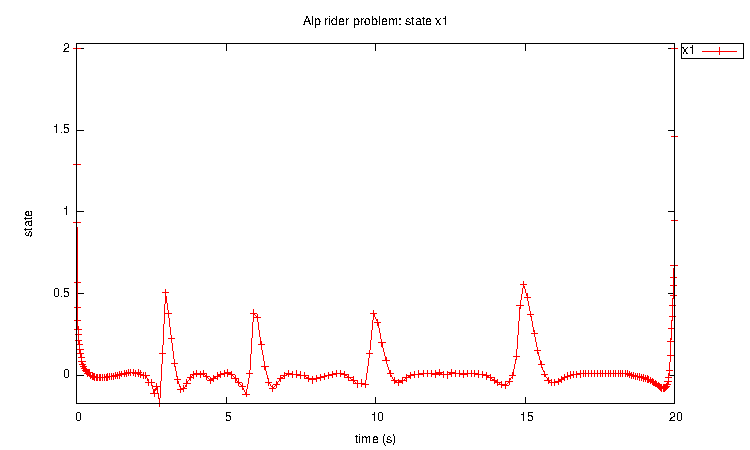
\includegraphics{../examples/alpine/alpine_state1}
  \caption{State $x_1(t)$ for the Alp rider problem}
  \label{alpine_state1}
\end{figure}

\begin{figure}
  \centering
  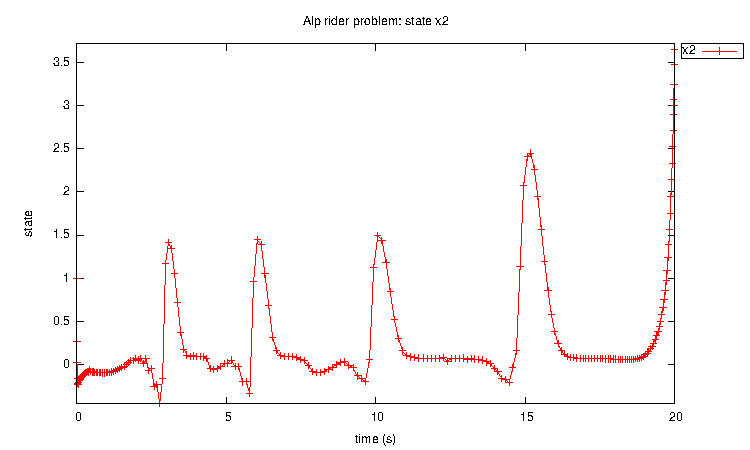
\includegraphics{../examples/alpine/alpine_state2}
  \caption{State $x_2(t)$ for the Alp rider problem}
  \label{alpine_state2}
\end{figure}

\begin{figure}
  \centering
  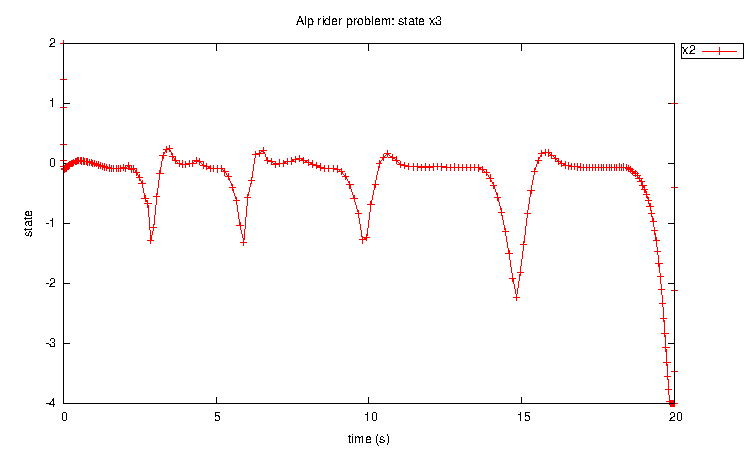
\includegraphics{../examples/alpine/alpine_state3}
  \caption{State $x_3(t)$ for the Alp rider problem}
  \label{alpine_state3}
\end{figure}

\begin{figure}
  \centering
  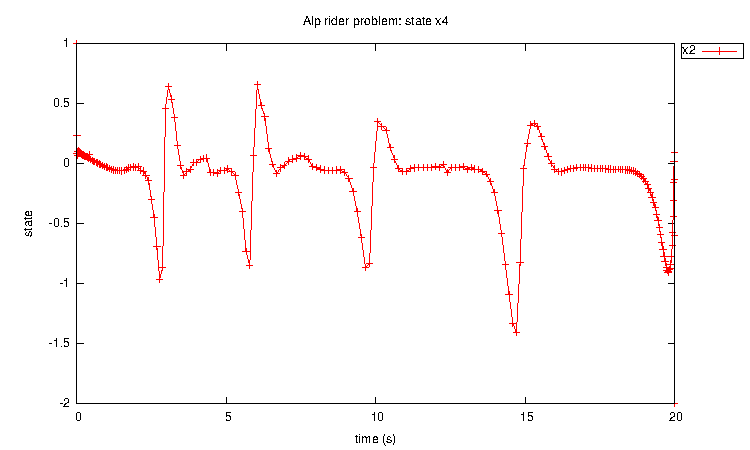
\includegraphics{../examples/alpine/alpine_state4}
  \caption{State $x_4(t)$ for the Alp rider problem}
  \label{alpine_state4}
\end{figure}


\begin{figure}
  \centering
  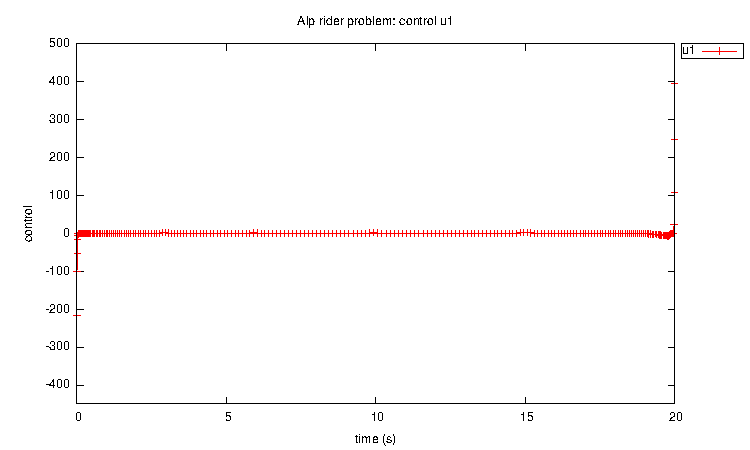
\includegraphics{../examples/alpine/alpine_control1}
  \caption{Control $u_1(t)$ for the Alp rider  problem}
  \label{alpine_control1}
\end{figure}

\begin{figure}
  \centering
  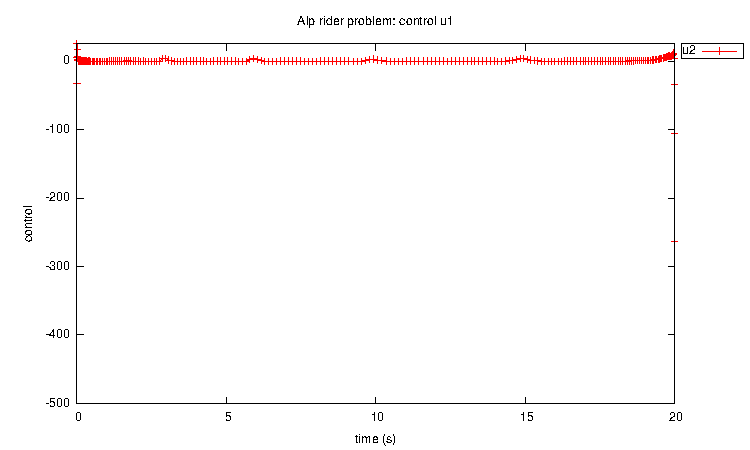
\includegraphics{../examples/alpine/alpine_control2}
  \caption{Control $u_2(t)$ for the Alp rider  problem}
  \label{alpine_control2}
\end{figure}


\section{Brachistochrone problem}
Consider the following optimal control problem.  Minimize the cost functional
\begin{equation}
  J = t_f
\end{equation}
subject to the dynamic constraints
\begin{equation}
  \begin{array}{lcl}
    \dot x & = & v \sin(\theta) \\
    \dot y & = & v \cos(\theta) \\
    \dot v & = & g \cos(\theta) 
  \end{array}
\end{equation}
and the boundary conditions
\begin{equation}
  \begin{array}{lcl}
    x(0) & = & 0 \\
    y(0) & = & 0 \\
    v(0) & = & 0 \\
    x(t_f) & = & 2 \\
    y(t_f) & = & 2 \\
  \end{array}
\end{equation}
where $g=9.8$. A version of this problem was originally formulated by Johann Bernoulli in 1696 and is referred to as the {\em Brachistochrone} problem.  The
\psopt code that solves this problem is shown below.  


\tiny
\begin{shadedframe}
\verbatiminput{../examples/brac1/brac1.cxx}
\end{shadedframe}
\normalsize

The output from \psopt is summarized in the box below and shown in Figures \ref{brac1_states}, \ref{brac1_control}, which contain the elements
of the state, and the control respectively.

\begin{shadedframe}
\verbatiminput{../examples/brac1/brac1.txt}
\end{shadedframe}

\begin{figure}
  \centering
  \includegraphics{../examples/brac1/brac1_states.pdf}
%  \includegraphics{../examples/brac1_states.eps}
  \caption{States for brachistochrone problem}
  \label{brac1_states}
\end{figure}


\begin{figure}
  \centering
  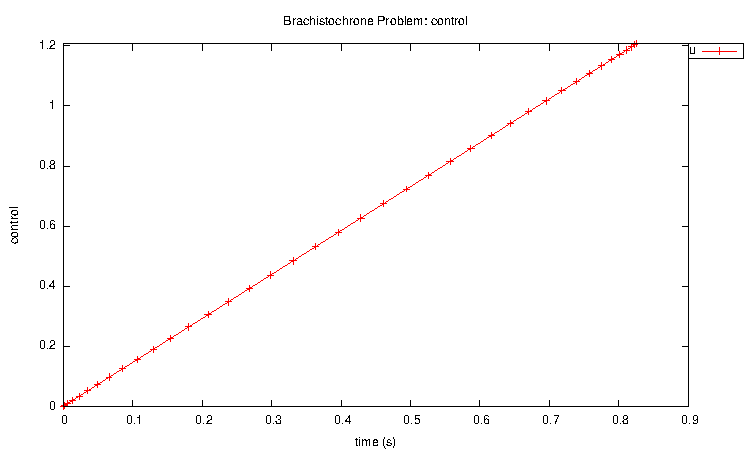
\includegraphics{../examples/brac1/brac1_control}
  \caption{Control for brachistochrone problem} 
  \label{brac1_control}
\end{figure}


\section{Breakwell problem}

Consider the following optimal control problem, which is known in the literature
as the Breakwell problem \cite{Bryson:75}. The problem benefits from having an analytical
solution, which is reported (with some errors) in the book by Bryson and Ho (1975). 
Minimize the cost functional.
\begin{equation}
  J = \int_{0}^{t_f} u(t)^2 \mathrm{d}t
\end{equation}
subject to the dynamic constraints
\begin{equation}
  \begin{array}{lcl}
    \dot x & = & v \\
    \dot v & = & u \\
  \end{array}
\end{equation}
the state dependent constraint
\begin{equation}
    x(t) \le l
\end{equation}
where $l = 0.1$, $t_f=1$.
and the boundary conditions
\begin{equation}
  \begin{array}{lcl}
    x(0) & = & 0 \\
    v(0) & = & 1 \\
    x(t_f) & = & 0 \\
    v(t_f) & = & -1 \\
  \end{array}
\end{equation}

The analytical solution of the problem (valid for $0\le l \le 1/6$) is given by:

\begin{equation}
 u(t) = \left\{  \begin{matrix} -\frac{2}{3l}(1-\frac{t}{3l}), & 0 \le t \le 3l \\ 0, & 3l \le t \le 1-3l \\ -\frac{2}{3l}(1-\frac{1-t}{3l}),  & 1-3l \le t \le 1 \end{matrix}  \right.
\end{equation}

\begin{equation}
 x(t) = \left\{  \begin{matrix} l\left( 1 -  \left(1-\frac{t}{3l}\right)^3 \right), & 0 \le t \le 3l \\ l, & 3l \le t \le 1-3l \\ l\left( 1 -  \left(1-\frac{1-t}{3l}\right)^3 \right),   & 1-3l \le t \le 1 \end{matrix}  \right.
\end{equation}

\begin{equation}
 v(t) = \left\{  \begin{matrix} \left(1-\frac{t}{3l}\right)^2, & 0 \le t \le 3l \\ 0, & 3l \le t \le 1-3l \\  \left(1-\frac{1-t}{3l}\right)^2 ,   & 1-3l \le t \le 1 \end{matrix}  \right.
\end{equation}


\begin{equation}
 \lambda_x(t) = \left\{  \begin{matrix} \frac{2}{9l^2}, & 0 \le t \le 3l \\ 0, & 3l \le t \le 1-3l \\  -\frac{2}{9l^2}, & 1-3l \le t \le 1 \end{matrix}  \right.
\end{equation}

\begin{equation}
 \lambda_v(t) = \left\{  \begin{matrix} \frac{2}{3l}(1-\frac{t}{3l}), & 0 \le t \le 3l \\ 0, & 3l \le t \le 1-3l \\  \frac{2}{3l}(1-\frac{1-t}{3l}), & 1-3l \le t \le 1 \end{matrix}  \right.
\end{equation}
where $\lambda_x(t)$ and $\lambda_v(t)$ are the costates. The analytical optimal value of the objective function is $J= 4/(9l) = 4.4444444$. The
\psopt code that solves this problem is shown below.  


\tiny
\begin{shadedframe}
\verbatiminput{../examples/breakwell/breakwell.cxx}
\end{shadedframe}
\normalsize

The output from \psopt is summarized in  the following box and shown in Figures \ref{breakwell_states} and \ref{breakwell_control}, which contain the elements of the state and the control, respectively,
and Figure \ref{breakwell_costates} which shows the costates. The figures include curves with the analytical solution for each variable, which is very close to the computed solution.

\begin{shadedframe}
\verbatiminput{../examples/breakwell/breakwell.txt}
\end{shadedframe}

\begin{figure}
  \centering
  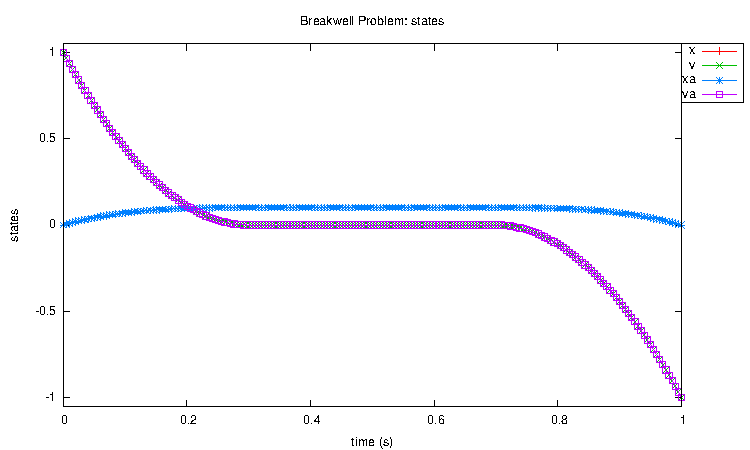
\includegraphics{../examples/breakwell/breakwell_states}
  \caption{States for Breakwell problem}
  \label{breakwell_states}
\end{figure}


\begin{figure}
  \centering
  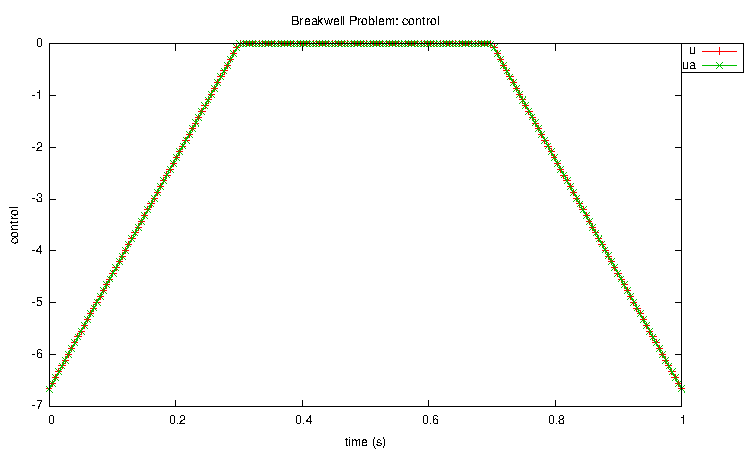
\includegraphics{../examples/breakwell/breakwell_control}
  \caption{Control for Breakwell problem}
  \label{breakwell_control}
\end{figure}

\begin{figure}
  \centering
  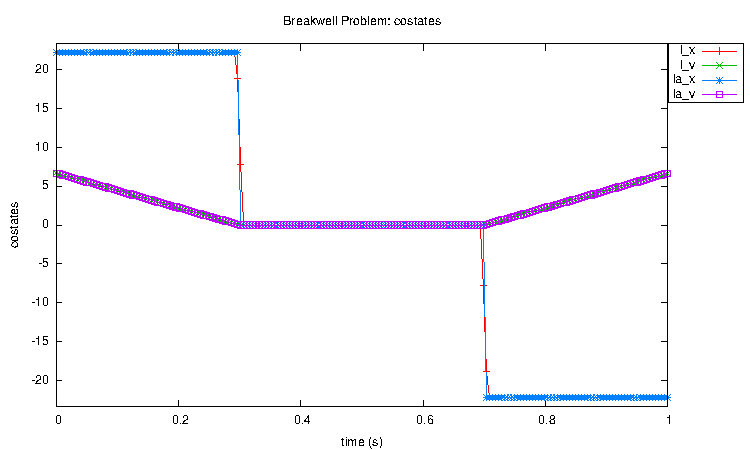
\includegraphics{../examples/breakwell/breakwell_costates}
  \caption{Costates for Breakwell problem}
  \label{breakwell_costates}
\end{figure}


\section{Bryson-Denham problem}

Consider the following optimal control problem, which is known in the literature
as the Bryson-Denham problem \cite{Bryson:69}.  Minimize the cost functional
\begin{equation}
  J = x_3(t_f)
\end{equation}
subject to the dynamic constraints
\begin{equation}
  \begin{array}{lcl}
    \dot x_1 & = & x_2 \\
    \dot x_2 & = & u \\
    \dot x_3 & = & \frac{1}{2} u^2 
  \end{array}
\end{equation}
the state bound
\begin{equation}
    0 \le  x_1 \le 1/9
\end{equation}
and the boundary conditions
\begin{equation}
  \begin{array}{lcl}
    x_1(0) & = & 0 \\
    x_2(0) & = & 1 \\
    x_3(0) & = & 0 \\
    x_1(t_f) & = & 0 \\
    x_2(t_f) & = & -1 \\
  \end{array}
\end{equation}
The
\psopt code that solves this problem is shown below.  


\tiny
\begin{shadedframe}
\verbatiminput{../examples/bryden/bryson_denham.cxx}
\end{shadedframe}
\normalsize

The output from \psopt is summarized in  the following box and shown in Figures \ref{bryden_states} and \ref{bryden_control}, which contain the elements of the state and the control, respectively.

\begin{shadedframe}
\verbatiminput{../examples/bryden/bryden.txt}
\end{shadedframe}

\begin{figure}
  \centering
  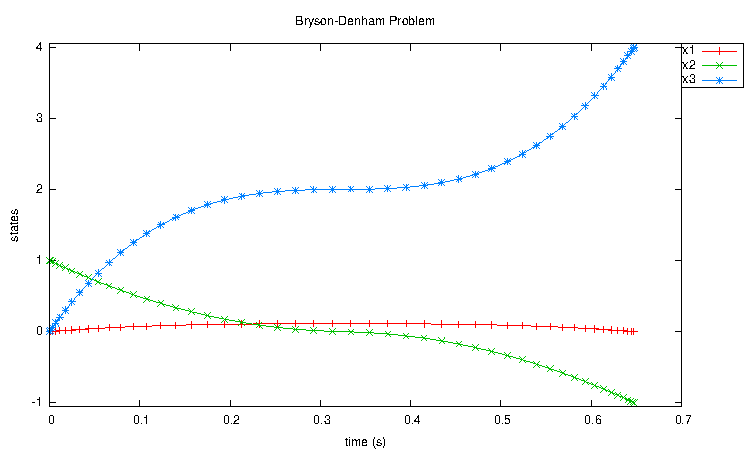
\includegraphics{../examples/bryden/bryden_states}
  \caption{States for Bryson Denham problem}
  \label{bryden_states}
\end{figure}


\begin{figure}
  \centering
  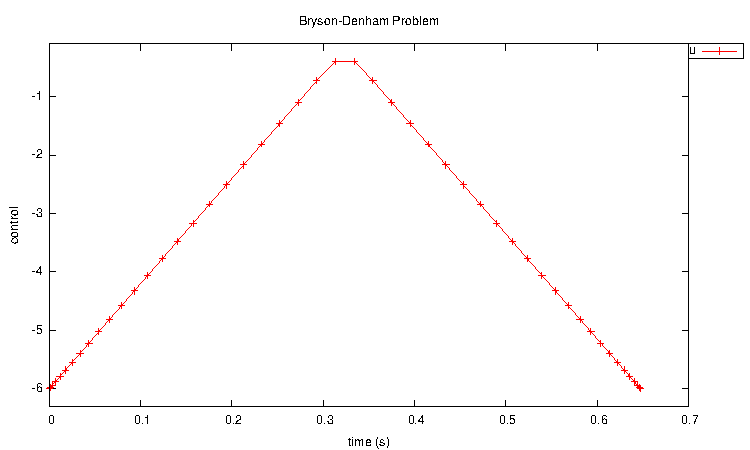
\includegraphics{../examples/bryden/bryden_control}
  \caption{Control for Bryson Denham problem}
  \label{bryden_control}
\end{figure}


\section{Bryson's maximum range problem}

Consider the following optimal control problem, which is known in the literature
as the Bryson's maximum range problem \cite{Bryson:69}.  Minimize the cost functional
\begin{equation}
  J = x(t_f)
\end{equation}
subject to the dynamic constraints
\begin{equation}
  \begin{array}{lcl}
    \dot x & = & v u_1 \\
    \dot y & = & v u_2 \\
    \dot v & = & a - g u_2
  \end{array}
\end{equation}
the path constraint
\begin{equation}
    u_1^2 + u_2^2 = 1
\end{equation}
and the boundary conditions
\begin{equation}
  \begin{array}{lcl}
    x(0) & = & 0 \\
    y(0) & = & 0 \\
    v(0) & = & 0 \\
    y(t_f) & = & 0.1 \\
  \end{array}
\end{equation}
where $t_f=2$, $g=1$ and $a=0.5g$. The
\psopt code that solves this problem is shown below.  

\tiny
\begin{shadedframe}
\verbatiminput{../examples/brymr/bryson_max_range.cxx}
\end{shadedframe}
\normalsize


The output from \psopt is summarized in the box below and shown in Figures \ref{brymr_states} and \ref{brymr_controls}, which contain the elements
of the state and the control, respectively.


\begin{shadedframe}
\verbatiminput{../examples/brymr/brymr.txt}
\end{shadedframe}

\begin{figure}
  \centering
  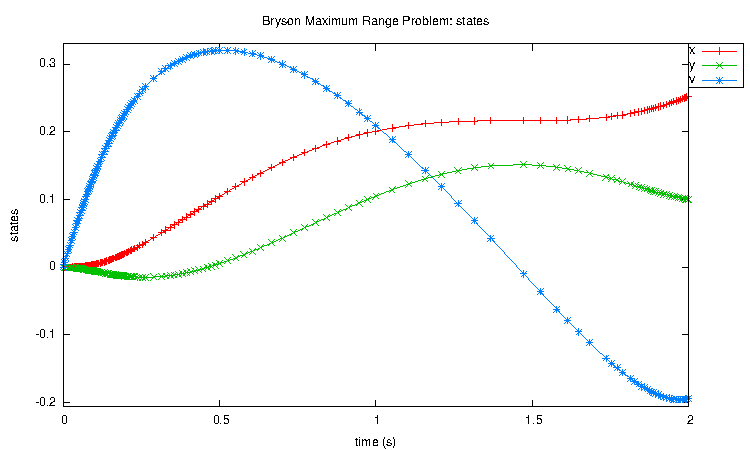
\includegraphics{../examples/brymr/brymr_states}
  \caption{States for Bryson's maximum range problem}
  \label{brymr_states}
\end{figure}


\begin{figure}
  \centering
  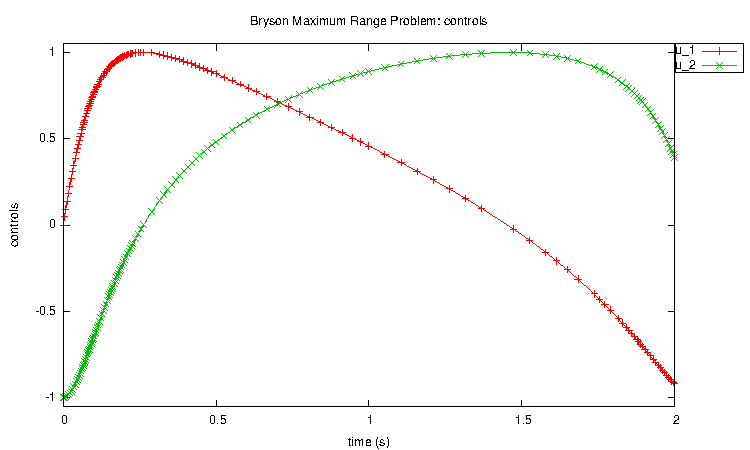
\includegraphics{../examples/brymr/brymr_controls}
  \caption{Controls for Bryson's maximum range problem}
  \label{brymr_controls}
\end{figure}



\section{Catalytic cracking of gas oil}

Consider the following optimization problem, which involves finding optimal static
parameters subject to dynamic constraints  \cite{Dolan:01}.  Minimize 
\begin{equation}
  J = \sum\limits_{i=1}^{21} (y_1(t_i) - y_{m,1}(i) )^2 + (y_2(t_i) - y_{m,2}(i) )^2 
\end{equation}
subject to the dynamic constraints
\begin{equation}
  \begin{array}{lcl}
    \dot y_1 & = & -(\theta_1 + \theta_3)y_1^2 \\
    \dot y_2 & = & \theta_1 y_1^2 - \theta_2 y_2
  \end{array}
\end{equation}
the parameter constraint
\begin{equation}
    \begin{aligned}
       \theta_1 &\ge 0 \\
       \theta_2 &\ge 0 \\
       \theta_3 &\ge 0  
    \end{aligned}
\end{equation}

Note that, given the 
nature of the problem, the parameter estimation facilities of \psopt are 
used in this example. In this case, the observations function is simple:

\[
    g( x(t), u(t), p, t ) = \left[ y_1\,\,\,y_2\right]^T
\]


The
\psopt code that solves this problem is shown below. The code includes
the values of the measurement vectors $y_{m,1}$, and $y_{m,2}$, as well
as the vector of sampling instants $\theta_i, i=1,\ldots,21$.

\tiny
\begin{shadedframe}
\verbatiminput{../examples/cracking/cracking.cxx}
\end{shadedframe}
\normalsize

The output from \psopt is summarized in the box below and shown in Figure \ref{fig:cracking_states},
which shows the states of the system. The optimal parameters found were:

\begin{equation}
\begin{aligned}
 \theta_1  = 11.40825702 \\
 \theta_2 = 8.123367918 \\	
 \theta_3 = 1.668727477 \\	
\end{aligned}
\end{equation}

\begin{shadedframe}
\verbatiminput{../examples/cracking/cracking.txt}
\end{shadedframe}

\begin{figure}
  \centering
  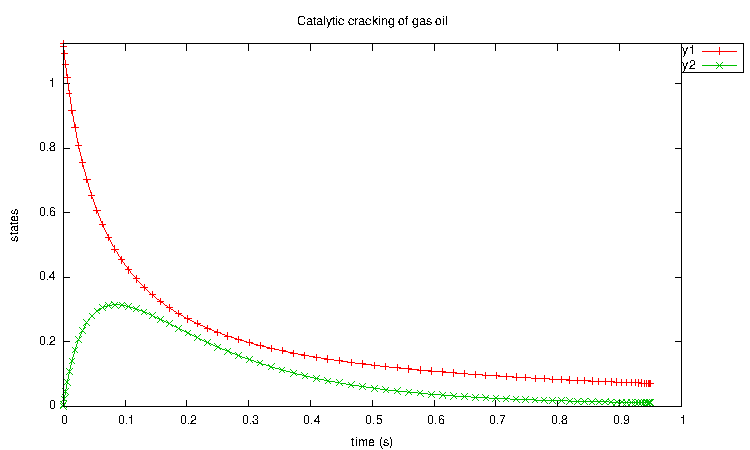
\includegraphics{../examples/cracking/cracking_states}
  \caption{States for catalytic cracking of gas oil problem}
  \label{fig:cracking_states}
\end{figure}

\section{Catalyst mixing problem}

Consider the following optimal control problem, which attempts to determine the optimal mixing policy
of two catalysts along the length of a tubular plug flow reactor involving several reactions
\cite{VonStryk:99}.  The catalyst mixing problem is a typical bang-singular-bang problem.  Minimize the cost functional
\begin{equation}
  J = -1 + x_1(t_f) + x_2(t_f)
\end{equation}
subject to the dynamic constraints
\begin{equation}
  \begin{array}{lcl}
    \dot x_1 & = & u(10x_2-x_1) \\
    \dot x_2 & = & u(x_1-10x_2) - (1-u)x_2
  \end{array}
\end{equation}
the boundary conditions
\begin{equation}
  \begin{array}{lcl}
    x_1(0) & = & 1 \\
    x_2(0) & = & 0 \\
    x_1(t_f) & \le & 0.95
  \end{array}
\end{equation}
and the box constraints:
\begin{equation}
   \begin{array}{lcl}
    0.9 & \le x_1(t) \le 1.0 \\
    0 & \le x_2(t) \le 0.1 \\
    0 & \le u(t)  \le 1 
  \end{array}
\end{equation}
where $t_f=1$. The
\psopt code that solves this problem is shown below.  

\tiny
\begin{shadedframe}
\verbatiminput{../examples/catmix/catmix.cxx}
\end{shadedframe}
\normalsize


The output from \psopt is summarised in the box below and shown in Figures \ref{fig:catmix_states} and \ref{fig:catmix_control}, which contain the elements
of the state and the control, respectively.

\begin{shadedframe}
\verbatiminput{../examples/catmix/catmix.txt}
\end{shadedframe}


\begin{figure}
  \centering 
  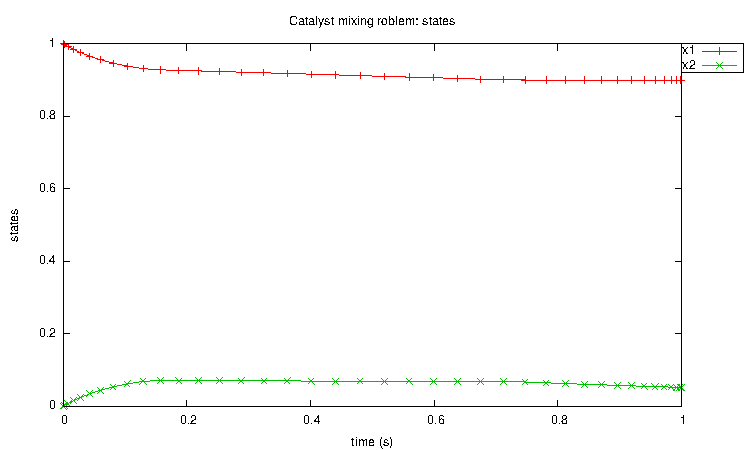
\includegraphics{../examples/catmix/catmix_states}
  \caption{States for catalyist mixing problem}
 \label{fig:catmix_states}
\end{figure}


\begin{figure}
  \centering
  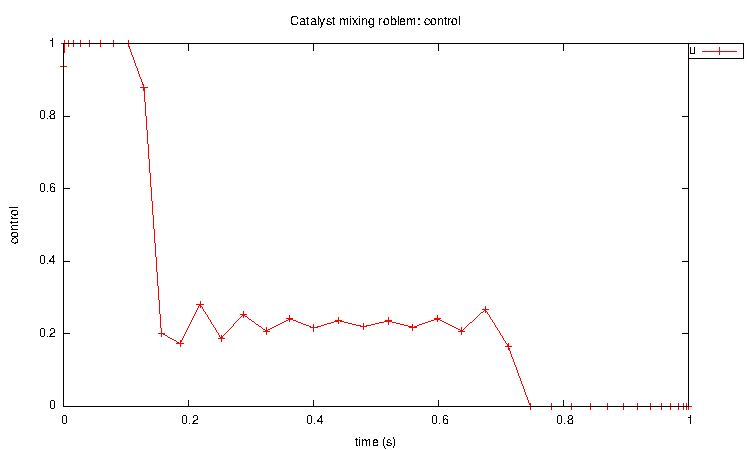
\includegraphics{../examples/catmix/catmix_control}
  \caption{Control for catalyst mixing problem}
 \label{fig:catmix_control}
\end{figure}


\section{Coulomb friction}

Consider the following optimal control problem, which consists of a system that exhibits Coulomb
friction  \cite{Luus:02}.  Minimize the cost:
\begin{equation}
  J = t_f
\end{equation}
subject to the dynamic constraints
\begin{equation}
  \begin{array}{lcl}
    \ddot  q_1 & = & ( -(k_1-k_2)q_1 + k_2 q_2 -\mu \mathrm{sign}( \dot q_1 ) + u_1)/m_1 \\
    \ddot  q_2 & = & ( k_2q_1 - k_2 q_2 -\mu \mathrm{sign}( \dot q_2 ) + u_2)/m_2
  \end{array}
\end{equation}
and the boundary conditions
\begin{equation}
  \begin{array}{lcl}
    q_1(0) & = & 0 \\
    \dot q_1(0) & = & -1 \\
    q_2(0) & = & 0 \\
    \dot q_2(0) & = & -2 \\
    q_1(t_f) & = & 1 \\
   \dot q_1(t_f) & = & 0 \\
   q_2(t_f)  & = & 2 \\
   \dot q_2(t_f) = 0 
  \end{array}
\end{equation}
where $k_1$ = 0.95, $k_2$=0.85, $\mu=1.0$, $m_1$=1.1, $m_2$=1.2. The
\psopt code that solves this problem is shown below.  

\tiny
\begin{shadedframe}
\verbatiminput{../examples/coulomb/coulomb.cxx}
\end{shadedframe}
\normalsize

The output from \psopt summarised in the box below and shown in Figures \ref{fig:coulomb_states} and \ref{fig:coulomb_controls}, which contain the elements
of the state and the control, respectively.

\begin{shadedframe}
\verbatiminput{../examples/coulomb/coulomb.txt}
\end{shadedframe}

\begin{figure}
  \centering 
  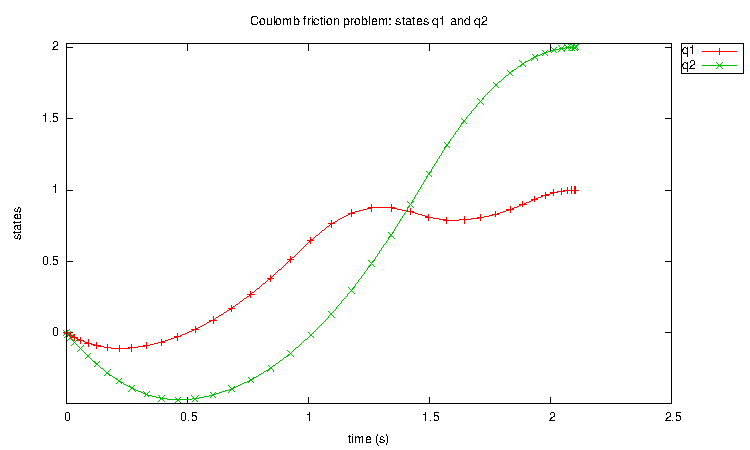
\includegraphics{../examples/coulomb/coulomb_states}
  \caption{States for Coulomb friction problem}
 \label{fig:coulomb_states}
\end{figure}


\begin{figure}
  \centering
  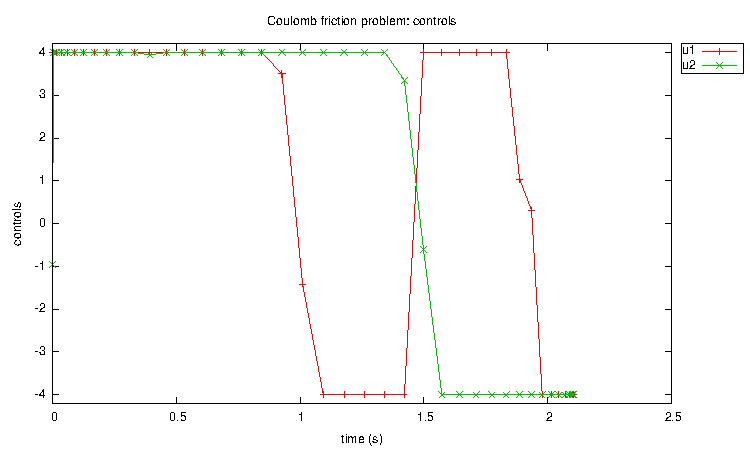
\includegraphics{../examples/coulomb/coulomb_control}
  \caption{Controls for Coulomb friction problem}
 \label{fig:coulomb_controls}
\end{figure}

\section{DAE index 3 parameter estimation problem}

Consider the following parameter estimation problem, which involves a differential-algebraic equation
of index 3 with four differential states and one algebraic state \cite{Schittkowski:02}.  

The dynamics consists of the differential equations
\begin{equation}
\begin{aligned}
  \dot x_1(t) &= x_3(t) \\
  \dot x_2(t) &= x_4(t) \\
  \dot x_3(t) &= \lambda(t) x_1(t) \\
  \dot x_4(t) &= \lambda(t) x_2(t) \\
\end{aligned}
\end{equation}
and the algebraic equation
\begin{equation}
  0 = L^2 - x_1(t)^2 - x_2(t)^2
\end{equation}
where $x_j(t), j=1,\ldots,4$ are the differential states, $\lambda(t)$ is an algebraic state (note
that algebraic states are treated as control variables), and $L$ is a parameter to be estimated.

The observations function is given by:
\begin{equation}
 \begin{aligned}
   y_1 &= x_1 \\
   y_2 &= x_2 
 \end{aligned}
\end{equation}

And the following least squares objective is minimised:
\begin{equation}
  J = \sum_{k=1}^{n_s} \left[ (y_1(t_k)-\hat{y}_1(t_k))^2 + (y_2(t_k)-\hat{y}_2(t_k))^2 \right] 
\end{equation}
where $n_s=20$, $t_1=0.5$ and $t_{20}=10.0$. 


The \psopt code that solves this problem is shown below.  

\tiny
\begin{shadedframe}
\verbatiminput{../examples/dae_i3/dae_i3.cxx}
\end{shadedframe}
\normalsize

The output from \psopt summarised in the box below and shown in Figures \ref{fig:dae_i3_x1} and \ref{fig:dae_i3_x2}, which
compare the observations with the estimated outputs, and \ref{fig:dae_i3_lambda}, which shows the algebraic state. The exact solution to the problem is $L=1$ and $\lambda(t)=-1$. The numerical solution obtained is
$L= 1.000000188$ and $\lambda(t)=-0.999868$. The 95\% confidence interval for the estimated parameter is $[0.9095289, \,\,\,1.090471]$

\begin{shadedframe}
\verbatiminput{../examples/dae_i3/dae_i3.txt}
\end{shadedframe}

\begin{figure}
  \centering 
  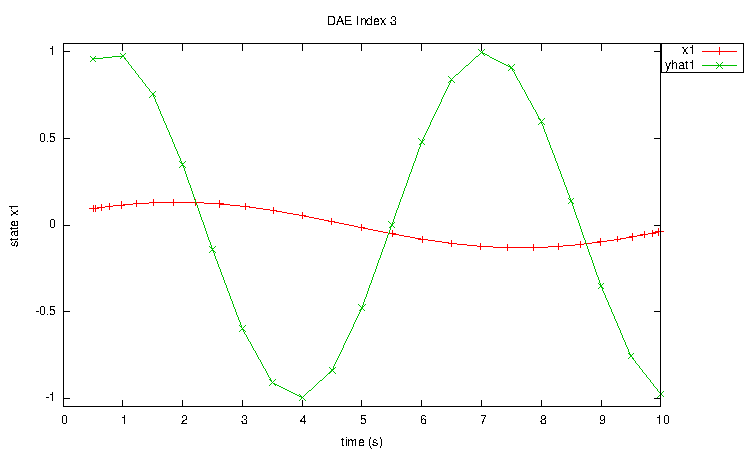
\includegraphics{../examples/dae_i3/x1}
  \caption{State $x_1$ and observations}
 \label{fig:dae_i3_x1}
\end{figure}


\begin{figure}
  \centering
  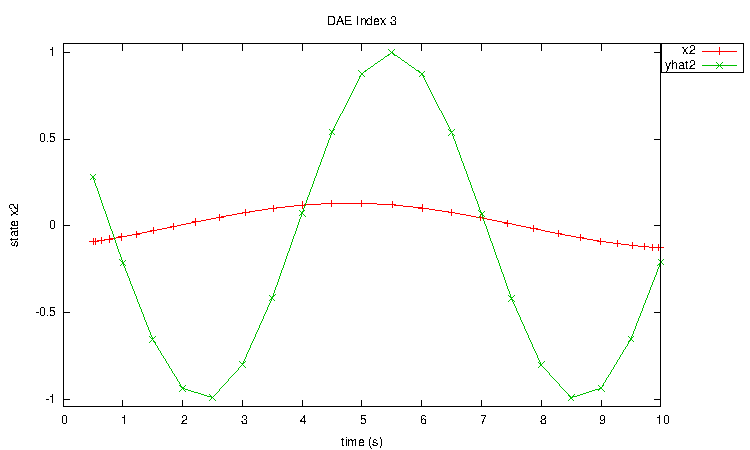
\includegraphics{../examples/dae_i3/x2}
  \caption{State $x_2$ and observations}
 \label{fig:dae_i3_x2}
\end{figure}

\begin{figure}
  \centering
  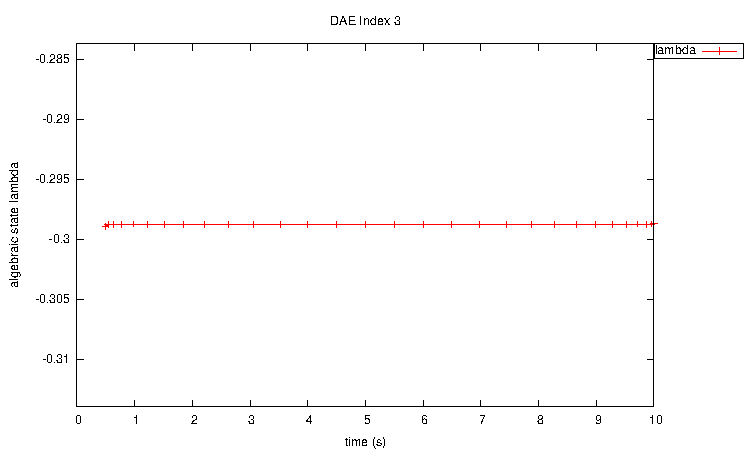
\includegraphics{../examples/dae_i3/lambda}
  \caption{Algebraic state $\lambda(t)$}
 \label{fig:dae_i3_lambda}
\end{figure}

\section{Delayed states problem 1}

Consider the following optimal control problem, which consists of a linear system
with delays in the state equations \cite{Luus:02}.  Minimize the cost functional:
\begin{equation}
  J = x_3(t_f)
\end{equation}
subject to the dynamic constraints
\begin{equation}
  \begin{array}{lcl}
    \dot x_1 & = & x_2(t) \\
    \dot x_2 & = & -10 x_1(t)-5 x_2(t)-2 x_1(t-\tau)-x_2(t-\tau)+u(t)\\
    \dot x_3 & = & 0.5 (10 x_1^2(t)+x_2^2(t)+u^2(t))
  \end{array}
\end{equation}
and the boundary conditions
\begin{equation}
  \begin{array}{lcl}
    x_1(0) & = & 1 \\
    x_2(0) & = & 1 \\
    x_3(0) & = & 0 
  \end{array}
\end{equation}
where $t_f=5$ and $\tau = 0.25$. The
\psopt code that solves this problem is shown below.  

\tiny
\begin{shadedframe}
\verbatiminput{../examples/delay1/delay1.cxx}
\end{shadedframe}
\normalsize

The output from \psopt summarised in the box below and shown in Figures \ref{fig:delay1_states} and \ref{fig:delay1_controls}, which contain the elements
of the state and the control, respectively. 	 
\begin{shadedframe}
\verbatiminput{../examples/delay1/delay1.txt}
\end{shadedframe}

\begin{figure}
  \centering 
  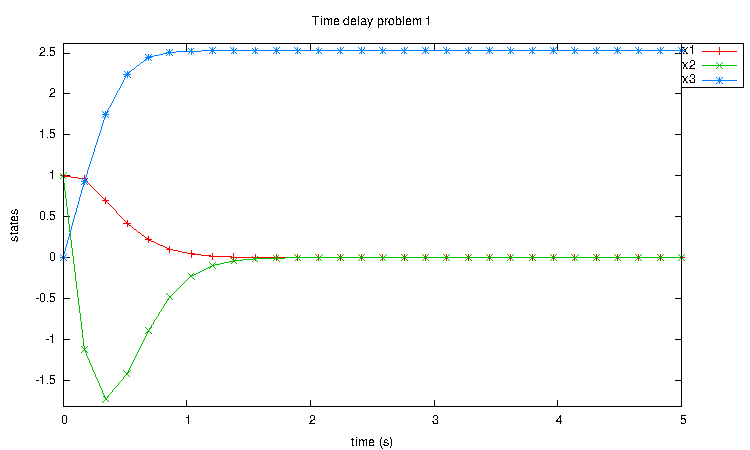
\includegraphics{../examples/delay1/delay1_states}
  \caption{States for time delay problem 1}
 \label{fig:delay1_states}
\end{figure}


\begin{figure}
  \centering
  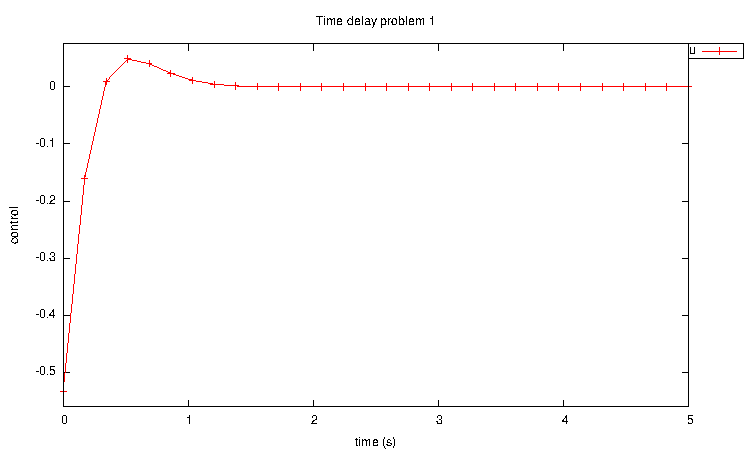
\includegraphics{../examples/delay1/delay1_controls}
  \caption{Control for time delay problem 1}
 \label{fig:delay1_controls}
\end{figure}

\section{Dynamic MPEC problem}

Consider the following optimal control problem, which involves special
handling of a system with a discontinuous right hand side \cite{Betts:10}.  
Minimize the cost functional:
\begin{equation}
  J = \left[ y(2)- 5/3\right]^2 + \int_0^2 y^2(t) \mathrm{d}t
\end{equation}
subject to 
\begin{equation}
  \begin{array}{lcl}
    \dot y & = & 2 - \mathrm{sgn}(y) \\
  \end{array}
\end{equation}
and the boundary condition
\begin{equation}
  \begin{array}{lcl}
    y(0) & = & -1 
  \end{array}
\end{equation}
Note that there is no control variable, and the analytical solution of this problem satisfies $\dot{y}(t)=3, \, 0 \le t \le 1/3$,
and $\dot{y}(t)=1, \, 1/3 \le t \le 2$.

In order to handle the discontinuous right hand side,  the problem is converted into the following equivalent
problem, which has three algebraic (control) variables. This type of problem is known in the literature as a dynamic MPEC problem.
\begin{equation}
  J = \left[ y(2)- 5/3\right]^2 + \int_0^2 \left( y^2(t) + \rho\left\{ p(t)[s(t)+1] +q(t)[1-s(t)] \right\} \right) \mathrm{d}t
\end{equation}
subject to 
\begin{equation}
  \begin{array}{lcl}
    \dot y & = & 2 - s(t) \\
     0 &=& -y(t) -p(t) + q(t)
  \end{array}
\end{equation}
the boundary condition
\begin{equation}
  \begin{array}{lcl}
    y(0) & = & -1 
  \end{array}
\end{equation}
and the bounds:
\begin{equation}
  \begin{array}{lcl}
    -1 &\le & s(t) \le  1, \\
     0 &\le & p(t), \\
     0 &\le & q(t).      
  \end{array}
\end{equation}

The \psopt code that solves this problem is shown below.  

\tiny
\begin{shadedframe}
\verbatiminput{../examples/mpec/mpec.cxx}
\end{shadedframe}
\normalsize

The output from \psopt summarised in the box below and shown in Figures \ref{fig:mpec_state}, \ref{fig:mpec_s}, \ref{fig:mpec_p}, and \ref{fig:mpec_q}.

\begin{shadedframe}
\verbatiminput{../examples/mpec/mpec.txt}
\end{shadedframe}

\begin{figure}
  \centering 
  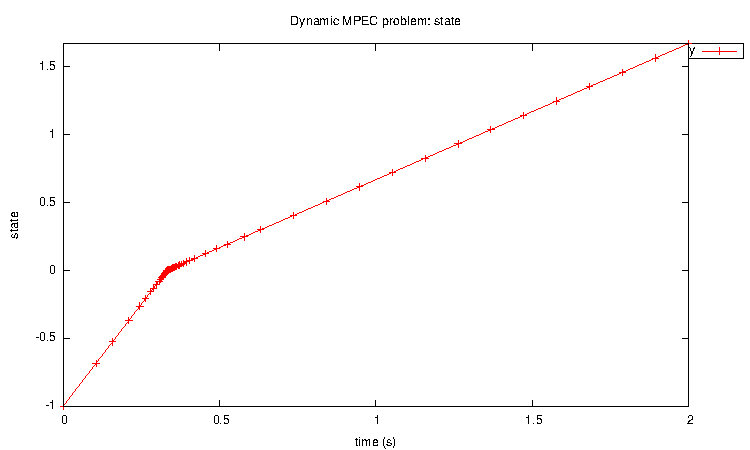
\includegraphics{../examples/mpec/y}
  \caption{State $y$ for dynamic MPEC problem}
 \label{fig:mpec_state}
\end{figure}


\begin{figure}
  \centering
  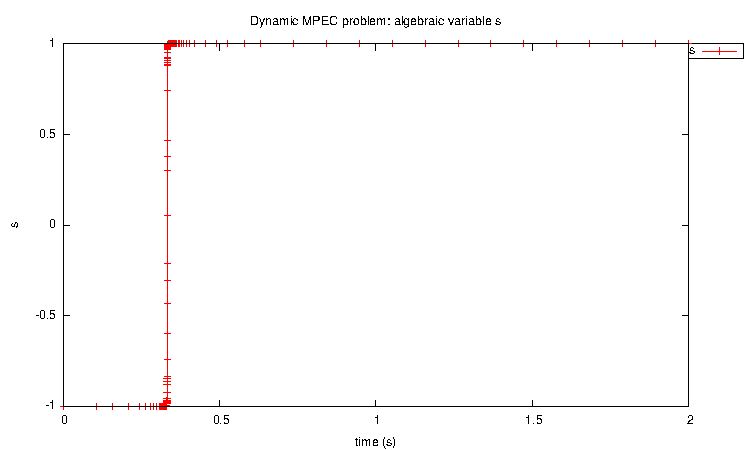
\includegraphics{../examples/mpec/s}
  \caption{Algebraic variable $s$ for dynamic MPEC problem}
 \label{fig:mpec_s}
\end{figure}

\begin{figure}
  \centering
  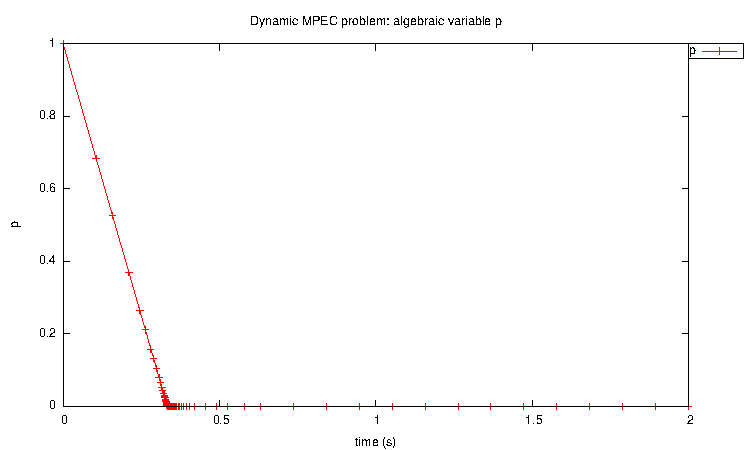
\includegraphics{../examples/mpec/p}
  \caption{Algebraic variable $p$ for dynamic MPEC problem}
 \label{fig:mpec_p}
\end{figure}

\begin{figure}
  \centering
  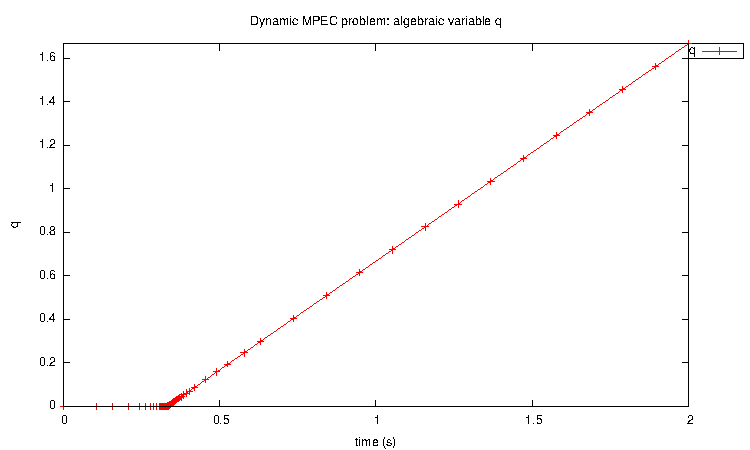
\includegraphics{../examples/mpec/q}
  \caption{Algebraic variable $q$ for dynamic MPEC problem}
 \label{fig:mpec_q}
\end{figure}



\section{Goddard rocket maximum ascent problem}

Consider the following optimal control problem, which is known in the literature
as the Goddard rocket maximum ascent problem \cite{Bryson:99}.  Find $t_f$ and $T(t) \in [t_0, t_f]$ 
to minimize the cost functional
\begin{equation}
  J = h(t_f)
\end{equation}
subject to the dynamic constraints
\begin{equation}
  \begin{array}{lcl}
   \dot v &=& \frac{1}{m}(T-D)-g \\
   \dot h &=& v \\
   \dot m &=& -\frac{T}{c}
  \end{array}
\end{equation}
the boundary conditions:
 \begin{equation}
  \begin{array}{lcl}
   h(0) &=& 0 \\
   v(0) &=& 1 \\
   m(0) &=& 1 \\
   m(t_f) &=& 0.6 
  \end{array}
\end{equation}
and the control bounds
\begin{equation}
  0 \le T(t) \le 3.5
\end{equation}
where
\begin{equation}
  \begin{array}{lcl}
   D &=& D_0 v^2\exp(-\beta h) \\
   g &=& 1/(h^2)
  \end{array},
\end{equation}
$D_0=310$, $\beta=500$, and $c = 0.5$, $0.1 \le t_f \le 1$. The
\psopt code that solves this problem is shown below.  

\tiny
\begin{shadedframe}
\verbatiminput{../examples/goddard/goddard.cxx}
\end{shadedframe}
\normalsize

The output from \psopt is summarised in the box below and  shown in Figures \ref{fig:goddard_states} and \ref{fig:goddard_control}, which contain the elements
of the state and the control, respectively.

\begin{shadedframe}
\verbatiminput{../examples/goddard/goddard.txt}
\end{shadedframe}

\begin{figure}
  \centering 
  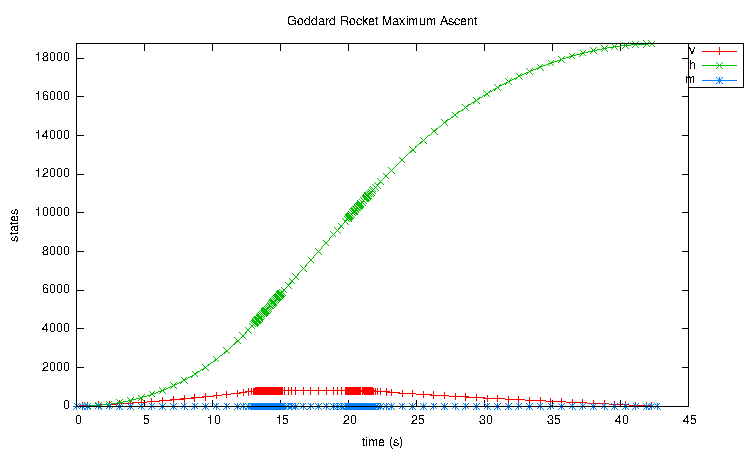
\includegraphics{../examples/goddard/goddard_states}
  \caption{States for Goddard rocket problem}
 \label{fig:goddard_states}
\end{figure}


\begin{figure}
  \centering
  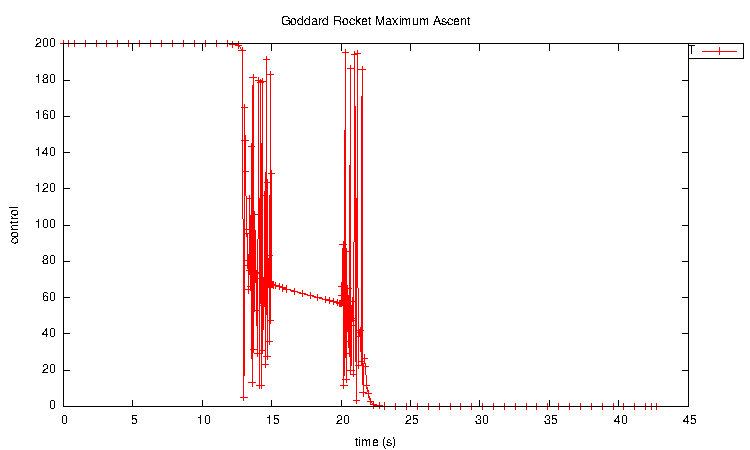
\includegraphics{../examples/goddard/goddard_control}
  \caption{Control for Goddard rocket problem}
 \label{fig:goddard_control}
\end{figure}



\section{Hang glider}

This problem is about the range maximisation of a hang glider in the presence of
a specified thermal draft \cite{Betts:10}.  Find $t_f$ and $C_L(t), t \in [0, t_f]$, 
to minimise,
\begin{equation}
  J = x(t_f)
\end{equation}
subject to the dynamic constraints
\begin{equation}
  \begin{array}{lcl}
   \dot x &=& v_x \\
   \dot y &=& v_y \\
   \dot v_x &=& \frac{1}{m}(-L \sin \eta - D \cos \eta)\\
   \dot v_y &=& \frac{1}{m}( L \cos \eta - D \sin \eta - W)
  \end{array}
\end{equation}
where
\begin{equation}
 \begin{aligned}
  C_D &= C_0 + k C_L^2 \\
    v_r&= \sqrt{ v_x^2 + v_y^2 }\\
    D &= \frac{1}{2} C_D \rho S v_r^2 \\
    L &= \frac{1}{2} C_L \rho S v_r^2 \\
    X &= \left( \frac{x}{R}-2.5 \right)^2 \\
    u_a &= u_M(1-X)\exp(-X) \\
    V_y &= v_y - ua \\
    \sin \eta  &= \frac{V_y}{v_r} \\
    \cos \eta  &= \frac{v_x}{v_r} \\
    W &= mg
 \end{aligned}
\end{equation}
The control is bounded as follows:
\begin{equation}
  0 \le C_L \le 1.4
\end{equation}
and the following boundary conditions:
\begin{equation}
 \begin{aligned}
  x(0)&= 0,  &x(t_f)= \mathrm{free} \\
  y(0)&=1000, &y(t_f)= 900 \\
  v_x(0)&=13.227567500, &v_x(t_f)=13.227567500\\
  v_y(0)&=-1.2875005200, &v_y(t_f)=-1.2875005200
 \end{aligned}
\end{equation}
With the following parameter values:
\begin{equation}
 \begin{aligned}
   u_M&= 2.5,  &m=100.0 \\
   R&= 100.0, &S=14,  \\
   C_0&= 0.034, &\rho=1.13 \\  
   k&= 0.069662, &g=9.80665
 \end{aligned}
\end{equation}


\psopt code that solves this problem is shown below.  

\tiny
\begin{shadedframe}
\verbatiminput{../examples/glider/glider.cxx}
\end{shadedframe}
\normalsize

The output from \psopt is summarised in the box below and  shown in Figures \ref{fig:glider_traj}, \ref{fig:glider_vel} and \ref{fig:glider_control}.

\begin{shadedframe}
\verbatiminput{../examples/glider/glider.txt}
\end{shadedframe}

\begin{figure}
  \centering 
  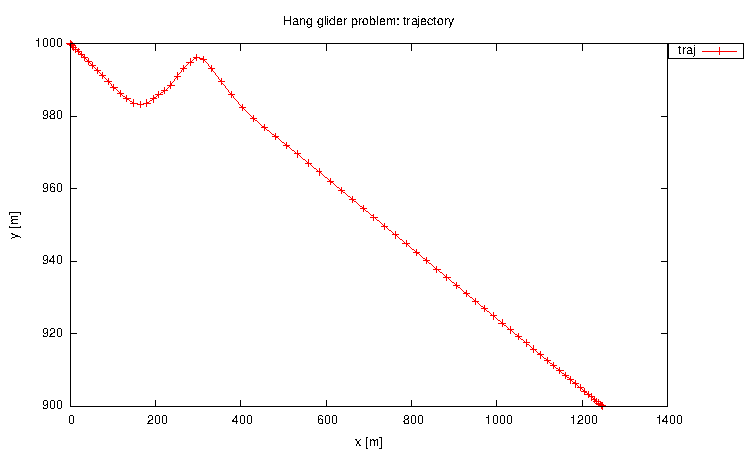
\includegraphics{../examples/glider/traj}
  \caption{$x-y$ trajectory for hang glider}
 \label{fig:glider_traj}
\end{figure}

\begin{figure}
  \centering 
  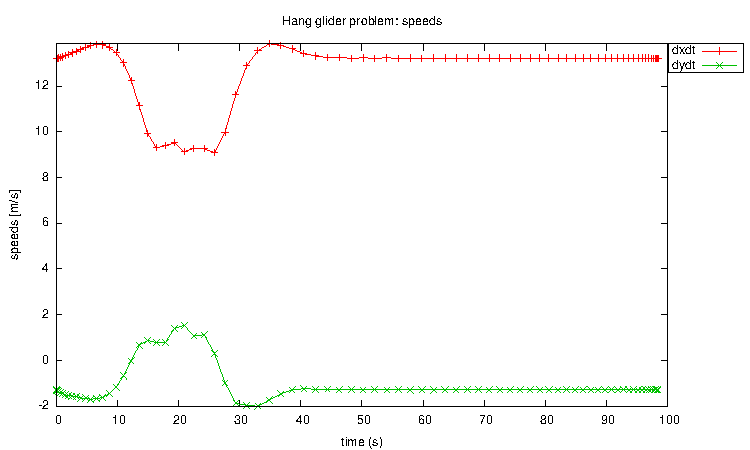
\includegraphics{../examples/glider/velocities}
  \caption{Velocities for hang glider}
 \label{fig:glider_vel}
\end{figure}



\begin{figure}
  \centering 
  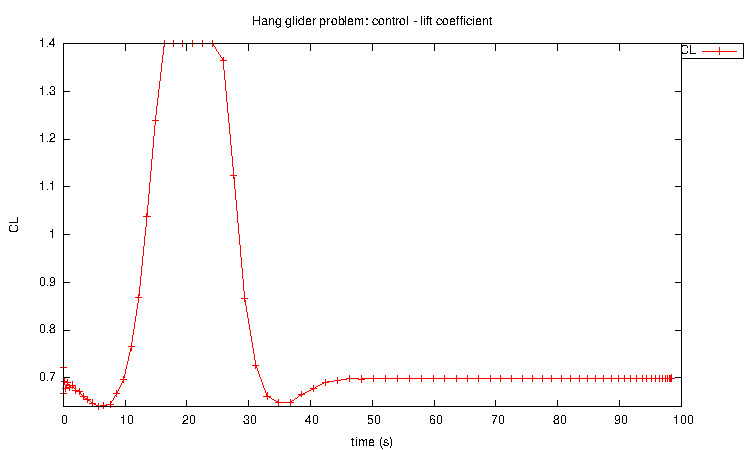
\includegraphics{../examples/glider/control}
  \caption{Lift coefficient for hang glider problem}
 \label{fig:glider_control}
\end{figure}


\section{Hanging chain problem}

Consider the following optimal control problem, which includes an integral constraint.
Minimize the cost functional
\begin{equation}
  J =  \int_0^{t_f} \left[ x \sqrt{1 + \left(\dot x \right)^2} \right]   dt
\end{equation}
subject to the dynamic constraint
\begin{equation}
    \dot x  =  u \\
\end{equation}
the integral constraint:
\begin{equation}
   \int_0^{t_f}   \left[ \sqrt{1 + \left(\frac{dx}{dt}\right)^2} \right]    dt = 4
\end{equation}
the boundary conditions
\begin{equation}
  \begin{array}{lcl}
    x(0) & = & 1 \\
    x(t_f) & = & 3 \\
  \end{array}
\end{equation}
and the bounds:
\begin{equation}
  \begin{aligned}
     -20 \le u(t) \le 20 \\
     -10 \le x(t) \le 10
  \end{aligned}
\end{equation}
where $t_f=1$. The
\psopt code that solves this problem is shown below.  

\tiny
\begin{shadedframe}
\verbatiminput{../examples/chain/chain.cxx}
\end{shadedframe}
\normalsize
The output from \psopt is summarized in the text box below and in Figure
\ref{chain_state}, which illustrates the shape of the hanging chain.

\small
\begin{shadedframe}
\verbatiminput{../examples/chain/chain.txt}
\end{shadedframe}
\normalsize

\begin{figure}
  \centering
  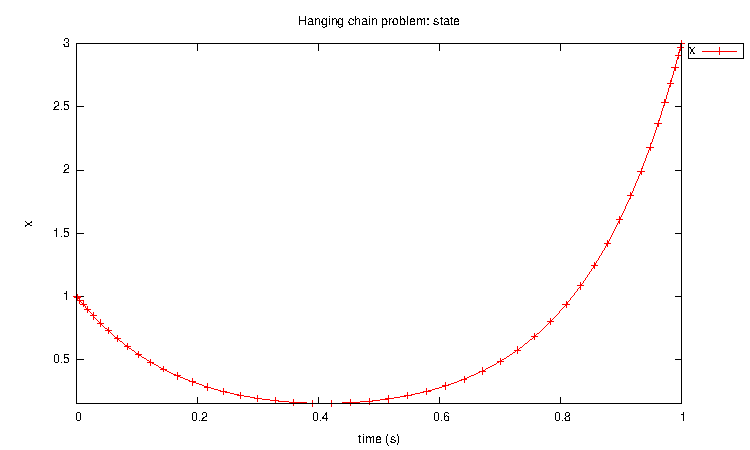
\includegraphics{../examples/chain/chain_state}
  \caption{State for hanging chain problem}
  \label{chain_state}
\end{figure}



\section{Heat difussion problem}

This example can be viewed as a simplified model for the heating of a probe in a kiln \cite{Betts:01}. 
The dynamics are a spatially discretized form of a partial differential equation, which is obtained by 
using the method of the lines. The problem is formulated on the basis of the state vector 
$\mathbf{x} = [x_1, \ldots, x_M]^T$ and the control vector $\mathbf{u}=[v_1, v_2, v_3]^T$, as follows
\[ 
  \min_{\mathbf{u}(t)} \,\, J = \frac{1}{2} \int_0^T \left\{ (x_N(t)-x_d(t))^2 + \gamma v_1(t)^2 \right\} \mathrm{d}t
\]
subject to the differential constraints
\[
\begin{aligned}
  \dot x_1 &= \frac{1}{(a_1 + a_2 x_1 )} \left[q_1 + \frac{1}{\delta^2}(a_3+a_4x_1)(x_2-2x_1+v_2) + a_4\left( \frac{x_2-x_1}{2\delta} \right)^2  \right] \\
  \dot x_i &= \frac{1}{(a_1 + a_2 x_i )} \left[q_i + \frac{1}{\delta^2}(a_3+a_4x_i)(x_{i+1}-2x_i+x_{i-1}) + a_4\left( \frac{x_{i+1}-x_{i-1}}{2\delta} \right)^2  \right] \\
  &\mathrm{for} \,\, i=2,\ldots,M-1 \\
  \dot x_M &= \frac{1}{(a_1 + a_2 x_M )} \left[q_M + \frac{1}{\delta^2}(a_3+a_4x_M)(v_3-2x_N+x_{M-1}) + a_4\left( \frac{v_3-x_{M-1}}{2\delta} \right)^2  \right] 
\end{aligned}
\]
the path constraints
\[
 \begin{aligned}
   0 &= g(x_1-v_1) - \frac{1}{2\delta}(a_3 + a_4 x_1)(x_2-v_2) \\
   0 &=  \frac{1}{2 \delta} (a_3 + a+4 x_M)(v_3 - x_{M-1})
 \end{aligned}
\]
the control bounds
\[
  u_L \le v_1 \le u_U
\]
and the initial conditions for the states:
\[
  x_i(0) = 2 + \cos(\pi z_i)
\]
where
\[
\begin{aligned}
  z_i &= \frac{i-1}{M-1}, \,\, i=1,\ldots,M \\
  x_d(t) &= 2- e^{\rho t} \\
  q(z,t) &= \left[ \rho( a_1 + 2 a_2) + \pi^2(a_3+2a_4) \right] e^{\rho t} \cos(\pi z) \\
         & - a_4 \pi^2 e^{2\pi t} + (2 a_4 \pi^2 + \rho a_2) e^{2 \rho t} \cos^2(\pi z)\\
  q_i &\equiv q(z_i, t), \,\, i=1,\ldots,M 
\end{aligned}
\]
with the parameter values $a_1=4$, $a_2=1$, $a_3=4$, $a_4=-1$, $u_U=0.1$, $\rho=-1$, $T=0.5$, $\gamma=10^{-3}$, 
$g=1$, $u_L=-\infty$.

A spatial discretization given by $M=10$ was used.  The problem was solved initially by using first 50 nodes, then the mesh was refined
to 60 nodes, and an interpolation of the previous solution was employed as an initial guess for the new solution.

The
\psopt code that solves this problem is shown below.  

\tiny
\begin{shadedframe}
\verbatiminput{../examples/heat/heat.cxx}
\end{shadedframe}
\normalsize

The output from \psopt is summarized the box below.  Figure \ref{heat_control} 
shows the control variable $v_1$ as a function of time.
Figure \ref{heat_surf} 
shows the resulting temperature distribution.

\begin{shadedframe}
\verbatiminput{../examples/heat/heat.txt}
\end{shadedframe}


%%\vspace{0cm}
\begin{figure}[htbp]
 \centerline{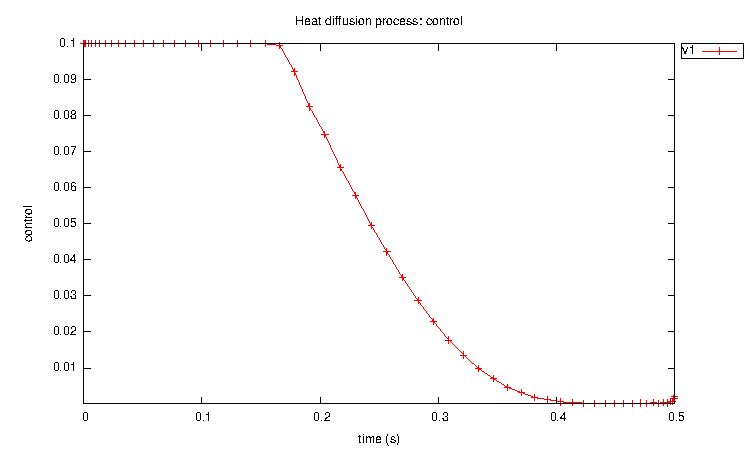
\includegraphics[height=9cm]{../examples/heat/heat_control}}
 \caption{Optimal control distribution for the heat diffusion process}
\label{heat_control}
\end{figure}



%%\vspace{0cm}
\begin{figure}[htbp]
 \centerline{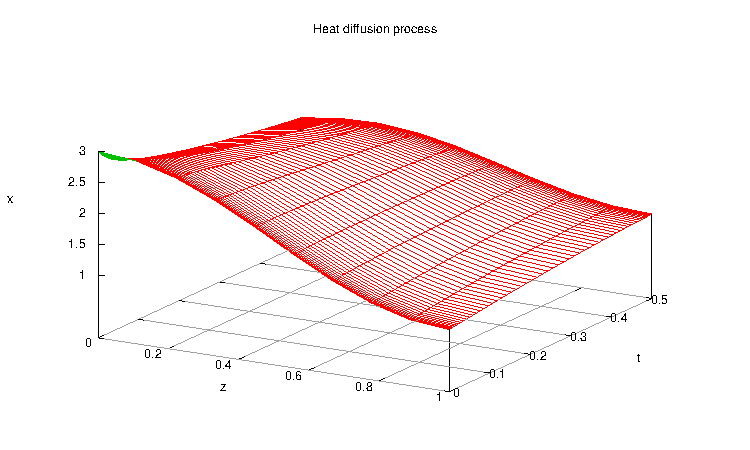
\includegraphics[height=9cm]{../examples/heat/heat_surf}}
\caption{Optimal temperature distribution for the heat diffusion process}
\label{heat_surf}
\end{figure}



\section{Hypersensitive problem}

Consider the following optimal control problem, which is known in the literature
as the hypesensitive optimal control problem \cite{Rao:00}.  Minimize the cost functional
\begin{equation}
  J = \frac{1}{2} \int_0^{t_f} [ x^2 + u^2 ] dt
\end{equation}
subject to the dynamic constraint
\begin{equation}
    \dot x  =  -x^3 + u \\
\end{equation}
and the boundary conditions
\begin{equation}
  \begin{array}{lcl}
    x(0) & = & 1.5 \\
    x(t_f) & = & 1 \\
  \end{array}
\end{equation}
where $t_f=50$. The
\psopt code that solves this problem is shown below.  

\tiny
\begin{shadedframe}
\verbatiminput{../examples/hyper/hypersensitive.cxx}
\end{shadedframe}
\normalsize
The output from \psopt is summarized the box below and shown in the following plots that contain the elements
of the state and the control, respectively.

\begin{shadedframe}
\verbatiminput{../examples/hyper/hyper.txt}
\end{shadedframe}



\begin{figure}
  \centering
  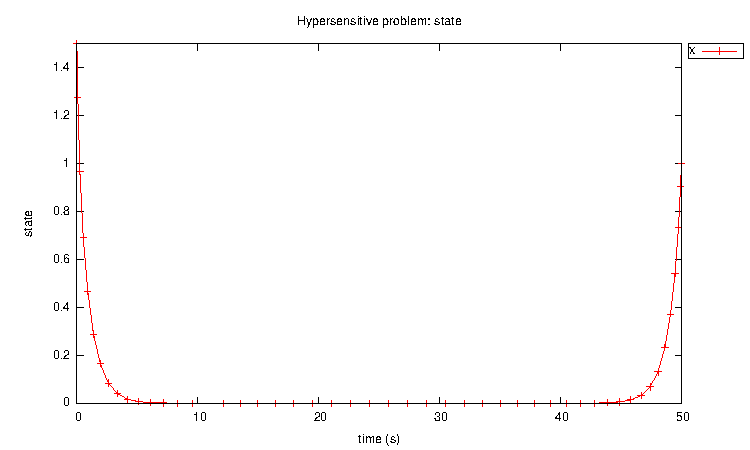
\includegraphics{../examples/hyper/hyper_state}
  \caption{State for hypersensitive problem}
\end{figure}


\begin{figure}
  \centering
  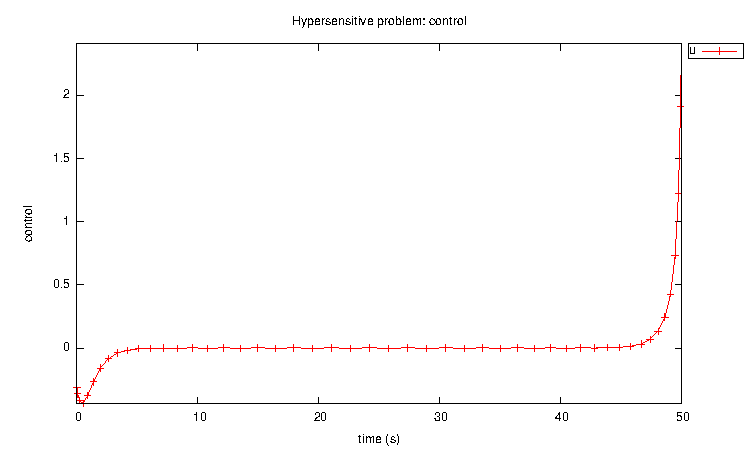
\includegraphics{../examples/hyper/hyper_control}
  \caption{Control for hypersensitive problem}
\end{figure}



\section{Interior point constraint problem}

Consider the following optimal control problem, which involves a scalar system with an interior
point constraint on the state \cite{Jennings:02}.  Minimize the cost functional
\begin{equation}
  J =  \int_0^{1} [ x^2 + u^2 ] dt
\end{equation}
subject to the dynamic constraint
\begin{equation}
    \dot x  =   u, \\
\end{equation}
the boundary conditions
\begin{equation}
  \begin{array}{lcl}
    x(0) & = & 1, \\
    x(1) & = & 0.75, \\
  \end{array}
\end{equation}
and the interior point constraint:
\begin{equation}
  x(0.75) = 0.9.
\end{equation}

The problem is divided into two phases and the interior point constraint is accommodated as an event constraint at the end of the first phase. The
\psopt code that solves this problem is shown below.  

\tiny
\begin{shadedframe}
\verbatiminput{../examples/ipc/interior_point.cxx}
\end{shadedframe}
\normalsize
The output from \psopt is summarized the box below and shown in the following plots that contain the elements
of the state and the control, respectively.

\begin{shadedframe}
\verbatiminput{../examples/ipc/ipc.txt}
\end{shadedframe}



\begin{figure}
  \centering
  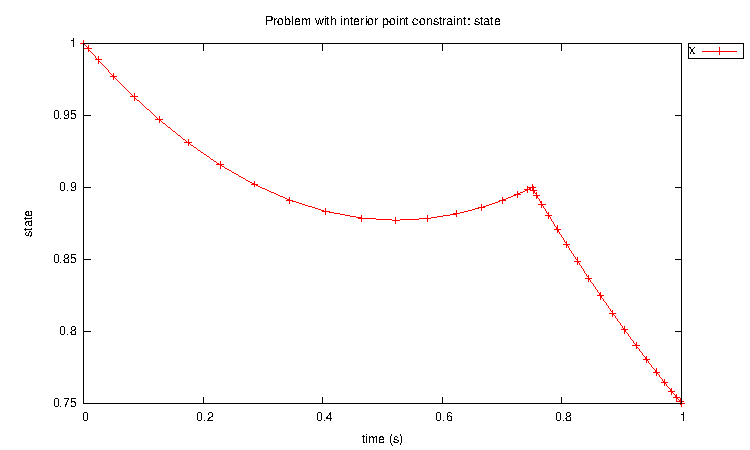
\includegraphics{../examples/ipc/ipc_state}
  \caption{State for interior point constraint problem}
\end{figure}


\begin{figure}
  \centering
  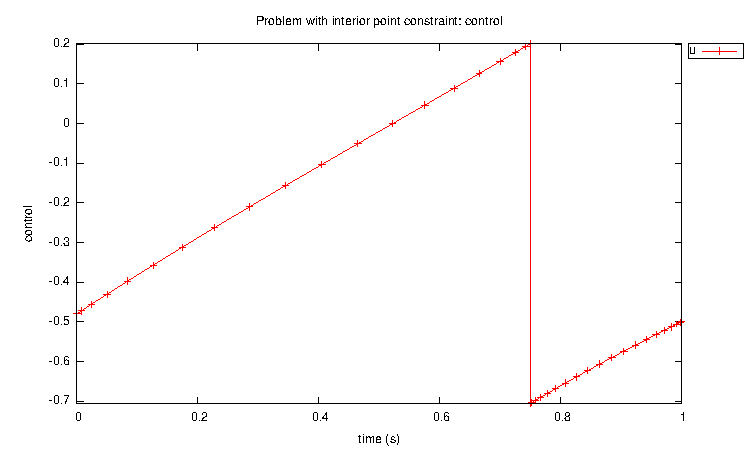
\includegraphics{../examples/ipc/ipc_control}
  \caption{Control for interior point constraint problem}
\end{figure}



\section{Isoperimetric constraint problem}

Consider the following optimal control problem, which includes an integral constraint.
Minimize the cost functional
\begin{equation}
  J =  \int_0^{t_f}  x^2(t)  dt
\end{equation}
subject to the dynamic constraint
\begin{equation}
    \dot x  =  -\sin(x) + u \\
\end{equation}
the integral constraint:
\begin{equation}
   \int_0^{t_f}   u^2(t)  dt = 10
\end{equation}
the boundary conditions
\begin{equation}
  \begin{array}{lcl}
    x(0) & = & 1 \\
    x(t_f) & = & 0 \\
  \end{array}
\end{equation}
and the bounds:
\begin{equation}
  \begin{aligned}
     -4 \le u(t) \le 4 \\
     -10 \le x(t) \le 10
  \end{aligned}
\end{equation}
where $t_f=1$. The
\psopt code that solves this problem is shown below.  

\tiny
\begin{shadedframe}
\verbatiminput{../examples/isop/isoperimetric.cxx}
\end{shadedframe}
\normalsize
The output from \psopt is summarized in the text box below and in Figures
\ref{isop_state} and \ref{isop_control}, which show the optimal state and control, respectively.

\small
\begin{shadedframe}
\verbatiminput{../examples/isop/isoperimetric.txt}
\end{shadedframe}
\normalsize

\begin{figure}
  \centering
  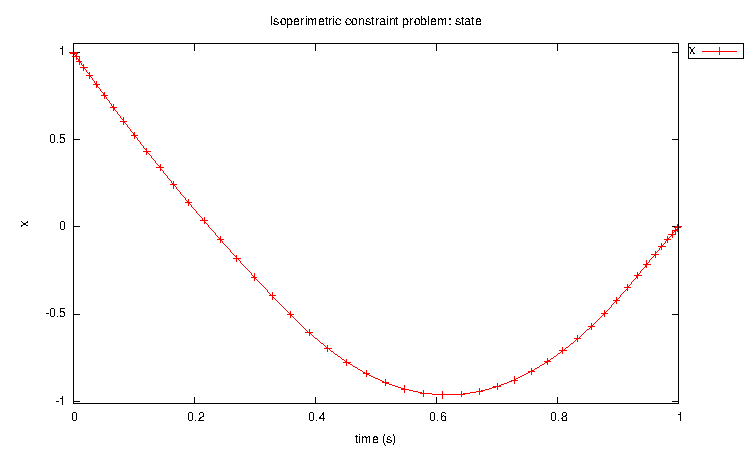
\includegraphics{../examples/isop/isop_state}
  \caption{State for isoperimetric constraint problem}
  \label{isop_state}
\end{figure}


\begin{figure}
  \centering
  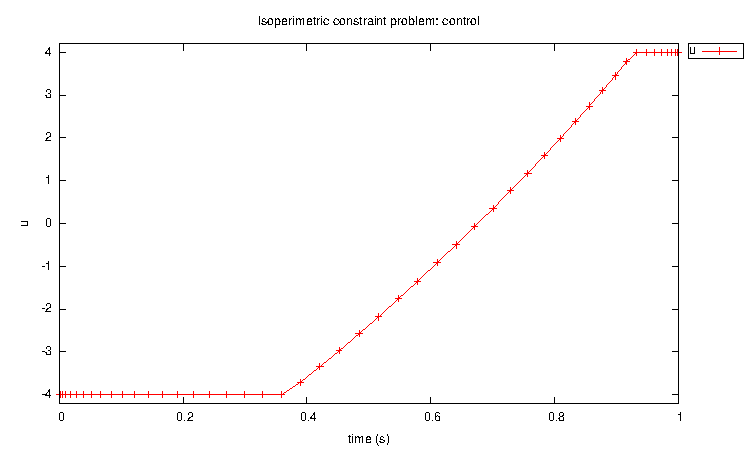
\includegraphics{../examples/isop/isop_control}
  \caption{Control for isoperimetric constraint problem}
 \label{isop_control}
\end{figure}



\section{Lambert's problem}

This example demonstrates the use of the \psopt for a classical orbit
determination problem, namely the determination of an orbit from two position vectors and
time (Lambert's problem) \cite{Vallado:01}. The problem is formulated as follows. Find $\mt{r}(t) \in [0,t_f]$ and $\mt{v}(t) \in [0,t_f]$ to minimise:

\begin{equation}
  J =  0
\end{equation}
subject to
\begin{equation}
  \begin{aligned}
     \dot{ \mt{r} }&= \mt{v} \\
     \dot{ \mt{v} }&= -\mu \frac{  \mt{r}    }{ || \mt{r} ||^3 }
  \end{aligned}
\end{equation}
with the boundary conditions:
\begin{equation}
\begin{aligned}
 \mt{r(0)} &= [15945.34\mathrm{E}3, 0.0, 0.0]^T \\
 \mt{r}(t_f) &= [ 12214.83899\mathrm{E}3, 10249.46731\mathrm{E}3, 0.0 ]^T
\end{aligned}
\end{equation}
where $\mt{r}=[x, y, z]^T$ (m) is a cartesian position vector, and $\mt{v}=[v_x, v_z, v_z]^T$ is the corresponding
velocity vector, $\mu=G M_e$, $G$ (m$^3$/(kg s$^2$)) is the universal gravitational constant and $M_e$ (kg) is the mass of Earth.


The \psopt code that solves this problem is shown below.  

\tiny
\begin{shadedframe}
\verbatiminput{../examples/lambert/lambert.cxx}
\end{shadedframe}
\normalsize
The output from \psopt is summarized in the text box below and in Figure
\ref{lambert_xy}, which show the trajectory from $\mt{r}(0)$ to $\mt{r}(t_f)$, respectively.

\small
\begin{shadedframe}
\verbatiminput{../examples/lambert/lambert.txt}
\end{shadedframe}
\normalsize

\begin{figure}
  \centering
  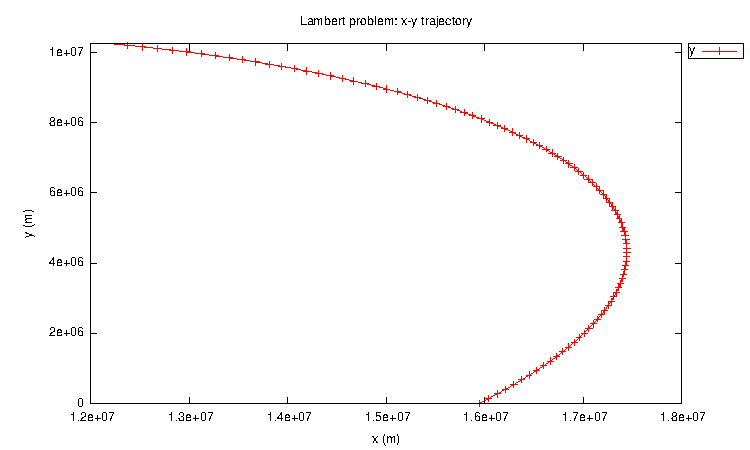
\includegraphics{../examples/lambert/lambert_xy.pdf}
  \caption{Trajectory between the initial and final positions for Lambert's problem}
  \label{lambert_xy}
\end{figure}

The resulting initial and final  velocity vectors are:

\begin{equation}
 \begin{aligned}
 \mt{v}(0) &= [2058.902605,  2915.961924, -6.878790137\mathrm{E}-13]^T 	 \\
  \mt{v}(t_f) &=[-3451.55505,  910.3192974,  -6.878787164\mathrm{E}-13 ]^T 	
 \end{aligned}
\end{equation}

\section{Lee-Ramirez bioreactor}


Consider the following optimal control problem, which is known in the literature
as the Lee-Ramirez bioreactor \cite{Luus:02, Rutquist:09}.  Find $t_f$ and $u(t) \in [0, t_f]$ 
to minimize the cost functional
\begin{equation}
  J = -x_1(t_f) x_4(t_f) + \int_{0}^{t_f} \rho [ \dot{u}_1(t)^2 + \dot{u}_2(t)^2  ] dt
\end{equation}
subject to the dynamic constraints
\begin{equation}
  \begin{aligned}
    \dot x_1 &=   u_1 + u_2; \\
    \dot x_2 &=  g_1 x_2 - \frac{ u_1+u_2}{x_1} x_2; \\
    \dot x_3 &=  100 \frac{u_1}{x_1} - \frac{u_1+u_2}{x_1} x_3 - (g_1/0.51) x_2; \\
    \dot x_4 &=  R_{fp} x_2 - \frac{u_1+u_2}{x_1} x_4; \\
    \dot x_5 &=  4 \frac{u_2}{x_1} - \frac{u_1+u_2}{x_1} x_5; \\
    \dot x_6 &=  -k_1 x_6;  \\
    \dot x_7 &=  k_2 (1-x_7). 
  \end{aligned}
\end{equation}
where $t_f=10$, $\rho = 1/N$, and $N$ is the number of discretization nodes,
\begin{equation}
 \begin{aligned}
    k_1 & = 0.09 x_5/(0.034 + x_5);\\
    k_2 &= k_1; \\
    g_1 & = (x_3/(14.35 + x_3(1.0+x_3/111.5)))(x_6 + 0.22 x_7/(0.22+x_5)); \\
    R_{fp} &= (0.233 x_3/(14.35 + x_3 (1.0+x_3/111.5))) ((0.0005+x_5)/(0.022+x_5));
 \end{aligned}
\end{equation}
the initial conditions:
 \begin{equation}
  \begin{array}{lcl}
   x_1(0) &=& 1 \\
   x_2(0) &=& 0.1 \\
   x_3(0) &=& 40 \\
   x_4(0) &=& 0  \\
   x_5(0) &=& 0 \\
   x_6(0) &=& 1.0 \\
   x_7(0) &=& 0 
  \end{array}
\end{equation}
The \psopt code that solves this problem is shown below.  


\tiny
\begin{shadedframe}
\verbatiminput{../examples/bioreactor/bioreactor.cxx}
\end{shadedframe}
\normalsize

The output from \psopt is summarised in the box below and shown in Figures \ref{fig:bioreactor_states} and \ref{fig:bioreactor_control}, which contain the elements
of the state and the control, respectively.

\begin{shadedframe}
\verbatiminput{../examples/bioreactor/bioreactor.txt}
\end{shadedframe}

\begin{figure}
  \centering 
  \includegraphics{../examples/bioreactor/bioreactor_states}
  \caption{States for the Lee-Ramirez bioreactor problem}
 \label{fig:bioreactor_states}
\end{figure}


\begin{figure}
  \centering
  \includegraphics{../examples/bioreactor/bioreactor_controls}
  \caption{Control for the Lee-Ramirez bioreactor problem}
 \label{fig:bioreactor_control}
\end{figure}


\section{Li's parameter estimation problem}

This is a parameter estimation problem with two parameters and three observed variables, which is presented b Li \emph{et. al} \cite{Li:2005}.

The dynamic equations are given by:
\begin{equation}
  \frac{d x} {dt} = M(t,p) x + f(t), \,\, t \in [0, \pi]
\end{equation}
with boundary condition:
\[
  x(0) + x(\pi) = (1 + e^{\pi})\left[ 1, \, 1, \, 1\right]^T
\]
where
\begin{equation}
  M(t,p) = \begin{bmatrix} 
   p_2 - p_1 \cos(p_2 t) & 0 & p_2 + p_1\sin(p_2t)  \\
   0 &   p_1 & 0 \\
   -p_2 + p_1 \sin(p_2 t) & 0 & p_2 + p_1 \cos(p_2 t) 
 \end{bmatrix}
\end{equation}
and
\begin{equation}
  f(t) =  \begin{bmatrix} 
    -1 + 19(\cos(t) - \sin(t)) \\
    -18 \\
    1- 19(\cos(t) + \sin(t))
  \end{bmatrix}
\end{equation}
and the observation functions are:
\begin{equation}
\begin{aligned}
  g_1 = x_1 \\
  g_2 = x_2 \\
  g_3 = x_3
\end{aligned}
\end{equation}
The trajectories of the dynamic system are characterised by rapidly varying fast and slow components if the difference between the two parameters $p_1$ and $p_2$ is large, which may cause numerical problems to some ODE solvers. 

The estimation data set is generated by adding Gaussian noise with standard deviation 1 around the solution $[x_1(t), x_2(t), x_3(t)]^T = [e^t,\, e^t,\, e^t]^T$, with $N=33$ equidistant samples within the interval $t=[0,\,\pi]$. The true values of the parameters are $p_1 = 19$ and $p_2 = 1$. The weights of the three observations are the same and equal to one. 

The solution is found using Legendre discretisation with 40 grid points. The code that solves the problem is shown below. The estimated parameter values and their 95$\%$ confidence limits for $n_s=129$ samples are shown in Table \ref{li-example-tab1}. Figure \ref{fig:param2_x1} shows the observations as well as the estimated values of variable $x_1$.

\tiny
\begin{shadedframe}
\verbatiminput{../examples/param2/param2.cxx}
\end{shadedframe}
\normalsize

\begin{table}
\label{li-example-tab1}
\caption{Estimated parameter values and 95 percent statistical confidence limits on estimated parameters} 
\begin{tabular}{llll}
\hline
Parameter &	Low Confidence Limit &	Value 	&	High Confidence Limit\\
$p_1$	&	1.907055e+01	&	1.907712e+01	&	1.908369e+01\\
$p_2$	&	9.984900e-01	&	9.984990e-01	&	9.985080e-01\\
\hline
\end{tabular}
\end{table}

\begin{figure}
  \centering 
  \includegraphics{../examples/param2/x1.pdf}
  \caption{Observations and estimated state $x_1(t)$}
 \label{fig:param2_x1}
\end{figure}



\section{Linear tangent steering problem}

Consider the following optimal control problem, which is known in the literature
as the linear tangent steering problem \cite{Betts:01}.  Find $t_f$ and $u(t) \in [0, t_f]$ 
to minimize the cost functional
\begin{equation}
  J = t_f
\end{equation}
subject to the dynamic constraints
\begin{equation}
  \begin{array}{lcl}
   \dot x_1 &=& x_2 \\
   \dot x_2 &=& a \cos(u) \\
   \dot x_3 &=& x_4 \\
   \dot x_4 &=& a \sin(u)\\
  \end{array}
\end{equation}
the boundary conditions:
 \begin{equation}
  \begin{array}{lcl}
   x_1(0) &=& 0 \\
   x_2(0) &=& 0 \\
   x_3(0) &=& 0 \\
   x_4(0) &=& 0  \\
   x_2(t_f) &=& 45.0 \\
   x_3(t_f) &=& 5.0 \\
   x_4(t_f) &=& 0.0 \\
  \end{array}
\end{equation}
The \psopt code that solves this problem is shown below.  

\tiny
\begin{shadedframe}
\verbatiminput{../examples/lts/lts.cxx}
\end{shadedframe}
\normalsize

The output from \psopt is summarised in the box below and shown in Figures \ref{fig:lts_states} and \ref{fig:lts_control}, which contain the elements
of the state and the control, respectively.

\begin{shadedframe}
\verbatiminput{../examples/lts/lts.txt}
\end{shadedframe}

\begin{figure}
  \centering 
  \includegraphics{../examples/lts/lts_states}
  \caption{States for the linear tangent steering problem}
 \label{fig:lts_states}
\end{figure}


\begin{figure}
  \centering
  \includegraphics{../examples/lts/lts_control}
  \caption{Control for the linear tangent steering problem}
 \label{fig:lts_control}
\end{figure}



\section{Low thrust orbit transfer}
\label{sec:ltot}

The goal of this problem is to compute an optimal low thrust policy for an spacecraft to go
from a standard space shuttle park orbit to a specified final orbit, while maximising the final 
weight of the spacecraft. The problem is described in detail by Betts \cite{Betts:01}. The problem
is formulated as follows. Find $\mt{u}(t) = [ u_r(t), u_{\theta}(t), u_h(t) ]^T, t \in [0, t_f]$,  
the unknown throtle parameter $\tau$, and the final time $t_f$, such that the following objective
function is minimised:

\begin{equation}
   J = -w(t_f)
\end{equation}
subject to the dynamic constraints:
\begin{equation}
\begin{aligned}
 \dot {\mt{y}} &= \mt{A}(\mt{y}) \Delta + \mt{b}\\
 \dot w &= -T[1+0.01 \tau]/ I_{sp}
\end{aligned}
\end{equation}
the path constraint:
\begin{equation}
  || u(t) ||^2 = 1
\end{equation}
and the parameter bounds:
\begin{equation}
 \tau_L \le \tau \le 0
\end{equation}
where $\mt{y} = [p, f, g, h, k, L, w]^T$ is the vector of modified equinoctial elements,  $w(t)$ is the 
weight of the spacecraft, $I_{sp}$ is the specific impulse of the engine, expressions for $\mt{A}(\mt{y})$ and $\mt{b}$ are given in \cite{Betts:01}, 
the disturbing acceleration $\Delta$ is given by:
\begin{equation}
 \Delta = \Delta_g + \Delta_T
\end{equation}
where $\Delta_g$ is the gravitational disturbing acceleration due to the oblatness of Earth (given in \cite{Betts:01}),
and $\Delta_T$ is the thurst acceleration, given by:
\[
  \Delta_T = \frac{g_0 T[1+0.01\tau]}{w} \mt{u}
\]
where $T$ is the maximum thrust, and $g_0$ is the mass to weight conversion factor.

The boundary conditions of the problem are given by:

\begin{equation}
 \begin{aligned}
    p(t_f) &= 40007346.015232 \,\,\mathrm{ft}\\
  \sqrt{f(t_f)^2+g(t_f)^2} &= 0.73550320568829 \\
 \sqrt{h(t_f)^2 + k(t_f)^2} &= 0.61761258786099 \\
 f(t_f) h(t_f) + g(t_f) k(t_f) &= 0 \\
 g(t_f) h(t_f) - k(t_f) f(t_f) &= 0 \\
 p(0) &= 21837080.052835 \mathrm{ft} \\
 f(0) &= 0 \\
 g(0) &= 0 \\
 h(0) &= 0 \\
 h(0) &= 0 \\ 
 k(0) &= 0 \\
 L(0) &= \pi \,\,(\mathrm{rad}) \\
 w(0) &= 1 \,\,(\mathrm{lb}) 
 \end{aligned}
\end{equation}
and the values of the parameters are: $g_0 = 32.174$ (ft/sec$^2$), $I_{sp}$ = 450 (sec), 
$T = 4.446618 \times 10^{-3}$  (lb),  $\mu = 1.407645794 \times 10^{16}$ (ft$^{3}$/sec$^{2}$),
$R_e = 20925662.73$ (ft), $J_2 =1082.639 \times 10^{-6} $,  $J_3 =-2.565 \times 10^{-6} $,
 $J_4 =-1.608 \times 10^{-6} $, $\tau_L = -50$.


An initial guess was computed by forward propagation from the initial conditions, assuming that
the direction of the thrust vector is parallel to the cartesian velocity vector, such that the initial control input was computed as follows:

\begin{equation}
 \mt{u}(t) = \mt{Q}_r^T \frac{\mt{v} }{ ||\mt{v}|| }
\end{equation}
where $\mt{Q}_r$ is a matrix whose columns are the directions of the rotating radial frame:
\begin{equation}
  \mt{Q}_r = \begin{bmatrix} \mt{i}_r &\mt{i}_\theta & \mt{i}_h \end{bmatrix}  = \begin{bmatrix} \frac{\mt{r}}{||\mt{r}||} &  \frac{(\mt{r}\times \mt{v})\times \mt{r}}{|| \mt{r} \times \mt{v} || || \mt{r}|| } & \frac{(\mt{r}\times \mt{v})}{|| \mt{r} \times \mt{v} || }\end{bmatrix}
\end{equation}


The problem was solved using local collocation (trapezoidal followed by Hermite-Simpson) with automatic mesh refinement. The \psopt code
that solves the problem is shown below.

\tiny
\begin{shadedframe}
\verbatiminput{../examples/lowthr/low_thrust.cxx}
\end{shadedframe}
\normalsize

The output from \psopt is summarised in the box below and shown in Figures \ref{fig:lowthr_x1}, to \ref{fig:lowthr_x6} and \ref{fig:lowthr_u1} 
to \ref{fig:lowthr_u3}, which contain the modified equinoctial
elements  and the controls, respectively.

\begin{shadedframe}
\verbatiminput{../examples/lowthr/lowthrust.txt}
\end{shadedframe}



\begin{table}
\caption{Mesh refinement statistics: Low thrust transfer problem}
\label{mesh_stats_Low th}
\renewcommand{\tabcolsep}{0.15cm}
\tiny
\begin{tabular}{llllllllllll}
Iter&DM&M&NV&NC&OE&CE&JE&HE&RHS&$\epsilon_{\max}$&CPU$_\mathrm{a}$ \\ \hline \\
1&TRP&80&803&653&1968&362&181&0&57558&2.208e-03&5.560e+00\\
2&TRP&98&983&797&118&119&110&0&23205&2.263e-03&4.060e+00\\
3&H-S&108&1404&984&145&146&141&0&47012&1.180e-03&7.650e+00\\
4&H-S&116&1508&1056&209&210&185&0&72660&3.514e-04&1.119e+01\\
\hline
CPU$_\mathrm{b}$ &-&-&-&-&-&-&-&-&-&-&8.250e+00\\
-&-&-&-&-&2440&837&617&0&200435&-&3.671e+01\\
\end{tabular}
\newline \\ \emph{Key}: Iter=iteration number, DM= discretization method, M=number of nodes, NV=number of variables, NC=number of constraints, OE=objective evaluations,  	              CE = constraint evaluations, JE = Jacobian evaluations, HE = Hessian evaluations, RHS = ODE right hand side 		      evaluations, $\epsilon_{\max}$ = maximum relative ODE error, CPU$_\mathrm{a}$ = CPU time in seconds spent by NLP algorithm, 		      CPU$_\mathrm{b}$ = additional CPU time in seconds spent by PSOPT
\normalsize
\end{table}



\begin{figure}
  \centering 
  \includegraphics{../examples/lowthr/lowthr_x1}
  \caption{Modified equinoctial element $p$}
 \label{fig:lowthr_x1}
\end{figure}


\begin{figure}
  \centering 
  \includegraphics{../examples/lowthr/lowthr_x2}
  \caption{Modified equinoctial element $f$}
 \label{fig:lowthr_x2}
\end{figure}

\begin{figure}
  \centering 
  \includegraphics{../examples/lowthr/lowthr_x3}
  \caption{Modified equinoctial element $g$}
 \label{fig:lowthr_x3}
\end{figure}

\begin{figure}
  \centering 
  \includegraphics{../examples/lowthr/lowthr_x4}
  \caption{Modified equinoctial element $h$}
 \label{fig:lowthr_x4}
\end{figure}

\begin{figure}
  \centering 
  \includegraphics{../examples/lowthr/lowthr_x5}
  \caption{Modified equinoctial element $k$}
 \label{fig:lowthr_x5}
\end{figure}

\begin{figure}
  \centering 
  \includegraphics{../examples/lowthr/lowthr_x6}
  \caption{Modified equinoctial element $L$}
 \label{fig:lowthr_x6}
\end{figure}


\begin{figure}
  \centering 
  \includegraphics{../examples/lowthr/lowthr_u1}
  \caption{Radial component of the thrust direction vector, $u_r$}
 \label{fig:lowthr_u1}
\end{figure}

\begin{figure}
  \centering 
  \includegraphics{../examples/lowthr/lowthr_u2}
  \caption{Tangential component of the thrust direction vector, $u_t$}
 \label{fig:lowthr_u2}
\end{figure}

\begin{figure}
  \centering 
  \includegraphics{../examples/lowthr/lowthr_u3}
  \caption{Normal component of the thrust direction vector, $u_h$}
 \label{fig:lowthr_u3}
\end{figure}

\section{Manutec R3 robot}

The DLR model 2  of the Manutec r3 robot, reported and validated by Otter and co-workers \cite{Otter:88, Franke:93}, describes the motion of three
links of the robot as a function of the control input signals of the robot drive:

\[
  \mt{M}(\mt{q}(t)) \ddot{\mt{q}}(t) = \mt{V}(\mt{q}(t), \dot{\mt{q}}(t) ) + \mt{G}(\mt{q}(t)) + \mt{D} \mt{u}(t)
\]
where $\mt{q} = [ q_1(t), q_2(t), q_3(t) ]^T$ is the vector of  relative angles between the links, the normalized torque controls are
$\mt{u}(t) = [ u_1(t), u_2(t), u_3(t) ]^T$, $\mt{D}$ is a diagonal matrix with constant values, $\mt{M}(\mt{q})$ is a
symmetric inertia matrix,  $\mt{V}(\mt{q}(t), \dot{\mt{q}}(t) )$ are the torques caused by coriolis and centrifugal
forces, $\mt{G}(\mt{q}(t))$ are gravitational torques. The model is described in detail in \cite{Otter:88} and is 
fully included in the code for this example\footnote{Dr. Martin Otter from DLR, Germany, 
has kindly authorised the author to publish  a translated form of subroutine R3M2SI as part of the \psopt distribution.}. 

The example reported here consists of a minimum energy point to point trajectory, so that the objective is to find $t_f$ and 
$\mt{u}(t) = [ u_1(t), u_2(t), u_3(t) ]^T$, $t \in [0, t_f]$ to minimise:


\begin{equation}
  J =  \int_0^{t_f} \mt{u}(t)^T \mt{u}(t)  \mathrm{d}t 
\end{equation}


The boundary conditions associated with the problem are:
\begin{equation}
  \begin{aligned}
  \mt{q}(0) &= \begin{bmatrix} 0 & -1.5 & 0  \end{bmatrix}^T \\
  \dot{\mt{q}}(0) &= \begin{bmatrix} 0 & 0 & 0  \end{bmatrix}^T \\
  \mt{q}(t_f) &= \begin{bmatrix}  1.0 & -1.95 & 1.0  \end{bmatrix}^T  \\
  \dot{\mt{q}}(t_f) &= \begin{bmatrix} 0 & 0 & 0  \end{bmatrix}^T 
  \end{aligned}
\end{equation}


The
\psopt code that solves this problem is shown below.  

\tiny
\begin{shadedframe}
\verbatiminput{../examples/manutec/manutec.cxx}
\end{shadedframe}
\normalsize
The output from \psopt is summarised in the box below and shown in Figures \ref{fig:manutec_positions}, \ref{fig:manutec_velocities} and \ref{fig:manutec_controls}, which contain the elements of
the position vector $\mt{q}(t)$, the velocity vector $\dot{\mt{q}}(t)$, and the controls $\mt{u}(t)$, respectively. 
The mesh refinement process is described in Table \ref{mesh_stats_manutec}.


\begin{shadedframe}
\verbatiminput{../examples/manutec/manutec.txt}
\end{shadedframe}

\begin{figure}
  \centering 
  \includegraphics{../examples/manutec/positions}
  \caption{States $q_1, q_2$ and $q_3$ for the Manutec R3 robot minimum energy  problem}
 \label{fig:manutec_positions}
\end{figure}

\begin{figure}
  \centering 
  \includegraphics{../examples/manutec/velocities}
  \caption{States $\dot q_1, \dot q_2$ and $\dot q_3$ for the Manutec R3 robot minimum energy  problem}
 \label{fig:manutec_velocities}
\end{figure}

\begin{figure}
  \centering 
  \includegraphics{../examples/manutec/controls}
  \caption{Controls $ u_1,  u_2$ and $u_3$ for the Manutec R3 robot minimum energy  problem}
 \label{fig:manutec_controls}
\end{figure}


\begin{table}
\caption{Mesh refinement statistics: Manutec R3 robot problem}
\label{mesh_stats_manutec}
\renewcommand{\tabcolsep}{0.15cm}
\tiny
\begin{tabular}{llllllllllll}
Iter&DM&M&NV&NC&OE&CE&JE&HE&RHS&$\epsilon_{\max}$&CPU$_\mathrm{a}$ \\ \hline \\
1&LGL-ST&20&182&133&43&43&35&0&860&4.676e-05&3.949e-01\\
2&LGL-ST&25&227&163&33&34&29&0&850&3.636e-05&4.298e-01\\
3&LGL-ST&35&317&223&37&38&30&0&1330&2.787e-05&7.294e-01\\
4&LGL-ST&49&443&307&18&19&17&0&931&7.660e-06&6.760e-01\\
\hline
CPU$_\mathrm{b}$ &-&-&-&-&-&-&-&-&-&-&2.475e+00\\
-&-&-&-&-&131&134&111&0&3971&-&4.705e+00\\
\end{tabular}
\newline \\ \emph{Key}: Iter=iteration number, DM= discretization method, M=number of nodes, NV=number of variables, NC=number of constraints, OE=objective evaluations,  	              CE = constraint evaluations, JE = Jacobian evaluations, HE = Hessian evaluations, RHS = ODE right hand side 		      evaluations, $\epsilon_{\max}$ = maximum relative ODE error, CPU$_\mathrm{a}$ = CPU time in seconds spent by NLP algorithm, 		      CPU$_\mathrm{b}$ = additional CPU time in seconds spent by PSOPT
\normalsize
\end{table}

\section{Minimum swing control for a container crane}


Consider the following optimal control problem \cite{Teo:91}, which seeks to minimise
the load swing of a container crane, while the load is transferred from one location
to another.  Find  $u(t) \in [0, t_f]$ to minimize the cost functional
\begin{equation}
\begin{aligned}
  J = 4.5 \int_{0}^{t_f} \left[ x_3^2(t) + x_6^2(t) \right] dt
\end{aligned}
\end{equation}
subject to the dynamic constraints
\begin{equation}
  \begin{array}{lcl}
   \dot x_1 &=& 9 x_4 \\
   \dot x_2 &=& 9 x_5  \\
   \dot x_3 &=& 9 x_6  \\
   \dot x_4 &=& 9(u_1 + 17.2656 x_3)   \\
   \dot x_5 &=& 9 u_2  \\
   \dot x_6 &=& - \frac{9}{x_2}\left[ u_1 + 27.0756x_3 +2x_5x_6 \right]   \\
  \end{array}
\end{equation}
the boundary conditions
 \begin{equation}
  \begin{array}{cccccc}
   x_1(0) &=& 0   & x_1(t_f) &=& 10 \\
   x_2(0) &=& 22  & x_2(t_f) &=& 14\\
   x_3(0) &=& 0   & x_3(t_f) &=& 0\\
   x_4(0) &=& 0   & x_4(t_f) &=& 2.5 \\
   x_5(0) &=& -1  & x_5(t_f) &=& 0\\
   x_6(0) &=& 0   & x_6(t_f) &=& 0 
  \end{array},
\end{equation}
and the  bounds
\begin{equation}
\begin{aligned}
  -2.83374 \le &u_1(t) \le 2.83374,\\
  -0.80865 \le &u_2(t) \le 0.71265,\\
-2.5 \le &x_4(t) \le 2.5,\\
-1 \le &x_5(t) \le 1.
\end{aligned}
\end{equation}

The
\psopt code that solves this problem is shown below.  

\tiny
\begin{shadedframe}
\verbatiminput{../examples/crane/crane.cxx}
\end{shadedframe}
\normalsize
The output from \psopt is summarised in the box below and shown in Figures \ref{fig:crane_states13}, \ref{fig:crane_states46} and \ref{fig:crane_controls}, which contain the elements
of the state $x_1$ to $x_3$, $x_4$ to $x_6$, and the controls, respectively.


\begin{shadedframe}
\verbatiminput{../examples/crane/crane.txt}
\end{shadedframe}

\begin{figure}
  \centering 
  \includegraphics{../examples/crane/crane_states13}
  \caption{States $x_1, x_2$ and $x_3$ for minimum swing crane control problem}
 \label{fig:crane_states13}
\end{figure}

\begin{figure}
  \centering 
  \includegraphics{../examples/crane/crane_states46}
  \caption{States $x_4, x_5$ and $x_6$ for minimum swing crane control problem}
 \label{fig:crane_states46}
\end{figure}


\begin{figure}
  \centering
  \includegraphics{../examples/crane/crane_controls}
  \caption{Controls for minimum swing crane control problem}
 \label{fig:crane_controls}
\end{figure}



\section{Minimum time to climb for a supersonic aircraft}


Consider the following optimal control problem, which finds the minimum time
to climb to a given altitude for a supersonic aircraft \cite{Betts:10}.  Minimize the cost functional
\begin{equation}
  J = t_f
\end{equation}
subject to the dynamic constraints
\begin{equation}
  \begin{array}{lcl}
    \dot h & = & v \sin \gamma \\
    \dot v & = & \frac{1}{m}\left[ T(M,h) \cos \alpha - D \right] - \frac{\mu}{(R_e+h)^2}\sin \gamma \\
    \dot \gamma & = & \frac{1}{m v}\left[ T(M,h) \sin \alpha + L \right] + \cos{\gamma} \left[ \frac{v}{(R_e+h)} - \frac{\mu}{v(R_e+h)^2} \right]\\
    \dot w &=& \frac{-T(M,h)}{I_{sp}}
  \end{array}
\end{equation}
where $h$ is the altitude (ft), $v$ is the velocity (ft/s),  $\gamma$ is the flight path
angle (rad), $w$ is the weight (lb), $L$ is the lift force, $D$ is the drag force (lb), $T$
is the thrust (lb), $M = v/c$ is the mach number, $m = w/g_0$ (slug) is the mass, $c(h)$ is the speed of
sound (ft/s), $R_e$ is the radious of Earth, and $\mu$ is the gravitational constant. The control input $\alpha$ is the angle of attack (rad). 

The speed of sound is given by:
\begin{equation}
  c=  20.0468 \sqrt{\theta}
\end{equation}
where $\theta=\theta(h)$ is the atmospheric temperature (K).

The aerodynamic forces are given by:

\begin{equation}
 \begin{aligned}
   D &= \frac{1}{2} C_D S \rho v^2 \\
   L &= \frac{1}{2} C_L S \rho v^2 \\
 \end{aligned}
\end{equation}
where
\begin{equation}
 \begin{aligned}
   C_L &= c_{L\alpha}(M) \alpha \\
   C_D &= c_{D0}(M) + \eta(M) c_{L\alpha}(M) \alpha^2 \\
 \end{aligned}
\end{equation}
where  $C_L$ and $C_D$ are aerodynamic lift and drag coefficients, $S$ is the
aerodynamic reference area of the aircraft, and $\rho=\rho(h)$ is the air density.

The boundary conditions are given by:
\begin{equation}
  \begin{aligned}
     h(0) & =0 \,\,\mathrm{(ft)}, \\
     h(t_f) &= 65600.0 \,\,\mathrm{(ft)} \\
     v(0) &= 424.260 \,\,\mathrm{(ft/s)}, \\
     v(t_f) & =968.148 \,\,\mathrm{(ft/s)} \\
     \gamma(0) &= \gamma(t_f)= 0 \,\,\mathrm{(rad)}\\
     w(0) = 42000.0 \,\,\mathrm{lb}
  \end{aligned}
\end{equation}

The parameter values are given by:
\begin{equation}
  \begin{aligned}
     S & = 530 \,\,\mathrm{(ft^2)}, \\
     I_{sp} &= 1600.0 \,\,\mathrm{(sec)} \\
     \mu &= 0.14046539 \,\,\times 10 ^{17} \,\,\mathrm{(ft^3/s^2)}, \\
     g_0 & = 32.174 \,\,\mathrm{(ft/s^2)} \\
     R_e &= 20902900 \,\,\mathrm{(ft)}\\
  \end{aligned}
\end{equation}

The variables $c_{L\alpha}(M)$, $c_{D0}(M)$, $\eta(M)$ are interpolated from 1-D tabular data which
is given in the code and also in \cite{Betts:10}, using spline interpolation, while the thrust $T(M,h)$ 
is interpolated from 2-D tabular data given in the code and in \cite{Betts:10}, using 2D spline interpolation.

The air density $\rho$ and the atmospheric temperature $\theta$ were calculated using the US Standard Atmosphere Model 1976\footnote{see http://www.pdas.com/programs/atmos.f90}, 
based on the standard temperature of 15 (deg C) at zero altitude and the standard air density of  1.22521 (slug/ft$^3$) at zero altitude.

The \psopt code that solves this problem is shown below.  

\tiny
\begin{shadedframe}
\verbatiminput{../examples/climb/climb.cxx}
\end{shadedframe}
\normalsize


The output from \psopt is summarized in the box below and Figures \ref{climb_alt}, to \ref{climb_alpha}. The results
can be compared with those presented in \cite{Betts:10}. Table \ref{mesh_stats_alpine} shows the mesh refinement history 
for this problem.


\begin{table}
\label{mesh_stats_Minimu}
\tiny
\begin{tabular}{llllllllllll}
Iter&Method&Nodes&NV&NC&OE&CE&JE&HE&RHS&$\epsilon_{\max}$&CPU(sec)\\ \hline \\
1&LGL-ST&80&322&247&747&746&89&0&59680&1.752e-03&8.020e+00\\
2&LGL-ST&90&362&277&70&71&55&0&6390&1.706e-03&6.890e+00\\
3&LGL-ST&100&402&307&28&29&28&0&2900&7.940e-04&4.810e+00\\
\hline
-&-&-&-&-&845&846&172&0&68970&-&1.972e+01\\
\end{tabular}
\newline \\ \emph{Key}: Iter=iteration number, NV=number of variables, NC=number of constraints, OE=objective evaluations,  	              CE = constraint evaluations, JE = Jacobian evaluations, HE = Hessian evaluations, RHS = ODE right hand side 		      evaluations, $\epsilon_{\max}$ = maximum relative ODE error, CPU(sec) = CPU time in seconds spent by nonlinear programming algorithm
\normalsize
\caption{Mesh refinement statistics: Minimum time to climb for a supersonic aircraft}
\end{table}

\begin{shadedframe}
\verbatiminput{../examples/climb/climb.txt}
\end{shadedframe}


\begin{figure}
  \centering
  \includegraphics{../examples/climb/climb_altitude}
  \caption{Altitude for minimum time to climb problem}
  \label{climb_alt}
\end{figure}


\begin{figure}
  \centering
  \includegraphics{../examples/climb/climb_velocity}
  \caption{Velocity for minimum time to climb problem}
  \label{climb_speed}
\end{figure}

\begin{figure}
  \centering
  \includegraphics{../examples/climb/climb_fpa}
  \caption{Flight path angle for minimum time to climb problem}
  \label{climb_fpa}
\end{figure}

\begin{figure}
  \centering
  \includegraphics{../examples/climb/weight.pdf}
  \caption{Weight for minimum time to climb problem}
  \label{climb_weight}
\end{figure}

\begin{figure}
  \centering
  \includegraphics{../examples/climb/alpha.pdf}
  \caption{Angle of attack ($\alpha$) for minimum time to climb problem}
  \label{climb_alpha}
\end{figure}



\section{Missile terminal burn maneouvre }


This example illustrates the design of a missile trajectory to strike a specified target from given initial 
conditions in minimum time \cite{Subchan:09}. Figure \ref{fig:missile} shows the variables associated with 
the dynamic model of the missile employed in this example, where $\gamma$ is the flight path angle, $\alpha$ 
is the angle of attack, $V$ is the missile speed, $x$ is the longitudinal position,  $h$ is the altitude, 
$D$ is the axial aerodynamic force, $L$ is the normal aerodynamic force, and $T$ is the thrust.
 
%\vspace{-1cm}
\begin{figure}[htbp] \label{fig:missile}
 \centerline{\includegraphics[height=10cm]{../examples/missile/missile}}
\caption{Ilustration of the variables associated with the missile model}
\end{figure}


The equations of motion of the missile are given by:

\[
 \begin{aligned}
   \dot \gamma & =  \frac{T-D}{mg} \sin \alpha + \frac{L}{mV} \cos \alpha - \frac{g \cos \gamma}{V}\\
   \dot V & = \frac{T-D}{m} \cos \alpha - \frac{L}{m} \sin \alpha - g \cos \gamma \\
   \dot x & = V \cos \gamma \\
   \dot h & = V \sin \gamma 
 \end{aligned}
\]

where

\[
                   \begin{aligned}
                   D &= \frac{1}{2} C_d \rho V^2 Sref \\
                   C_d &= A_1 \alpha^2 + A_2 \alpha + A_3 \\
                   L &= \frac{1}{2} C_l \rho V^2 Sref \\
                   C_l &= B_1 \alpha + B_2 \\
                   \rho &= C_1 h^2 + C_2 h + C_3
                   \end{aligned}
\] 
where all the model parameters are given in Table \ref{tab:missile_param}.
The initial conditions for the state variables are:

\[\begin{aligned}
\gamma(0) &= 0  \\
V(0) &= 272 \mathrm{m/s}  \\
x(0) &= 0 \mathrm{m} \\
h(0) &= 30 \mathrm{m} 
\end{aligned}
\]
The terminal conditions on the states are:

\[ \begin{aligned}
\gamma(t_f) &= -\pi/2  \\
V(t_f) &= 310 \mathrm{m/s}  \\
x(t_f) &= 10000 \mathrm{m} \\
h(t_f) &= 0 \mathrm{m} 
\end{aligned}
\]
The problem constraints are given by:

\[
\begin{aligned}
  200 \le  &V \le 310 \\
  1000 \le  &T \le 6000 \\
  -0.3 \le  &\alpha \le 0.3 \\
  -4 \le & \frac{L}{mg} \le 4\\
  &h \ge 30 \, \,(\mathrm{for} \,  x \le 7500 \mathrm{m}) \\
  &h \ge 0 \, \,(\mathrm{for} \,  x > 7500 \mathrm{m}) \\
\end{aligned}
\]

\begin{table} 
\caption{Parameters values of the missile model} \label{tab:missile_param}
\begin{center}
\begin{tabular}{lll}
Parameter & Value  & Units \\
$m$         & 1005   & kg \\
$g$         & 9.81   &m/s$^2$ \\
$S_{\mathrm{ref}}$ & 0.3376 &  m$^2$ \\
$A_1$ & -1.9431 \\
$A_2$ & -0.1499 \\
$A_3$ & 0.2359 \\
$B_1$ & 21.9 \\
$B_2$ &  0 \\
$C_1$ & $3.312 \times 10^{-9}$ & kg/m$^5$\\
$C_2$ & $-1.142 \times 10^{-4}$ & kg/m$^4$\\
$C_3$ & 1.224 & kg/m$^3$\


\end{tabular}
\end{center}
\end{table}

Note that the path constraints on the altitude are non-smooth.
Given that non-smoothness causes problems with nonlinear programming, the constraints on the altitude
were approximated by a single smooth constraint:
\[
   \mathcal{H}_\epsilon(x-7500)) h(t) +   [1-\mathcal{H}_\epsilon(x-7500)] [h(t)-30] \ge 0
\]
where $\mathcal{H}_\epsilon(z)$ is a smooth version of the Heaviside function, which
is computed as follows:
\[
    \mathcal{H}_\epsilon(z) =  0.5( 1 + \tanh(z/\epsilon) )
\]
where $\epsilon>0$ is a small number.

The problem is solved by using automatic mesh refinement starting with 50 nodes. The final
solution, which is found after six mesh refinement iterations, has 85 nodes. Figure \ref{missile_alt_vs_x} 
shows the missile altitude as a function of the longitudinal position.
Figures \ref{missile_speed} and \ref{missile_alpha} 
show, respectively, the missile speed and angle of attack as functions  of time.
The output from \psopt is summarised in the box below.


\begin{shadedframe}
\verbatiminput{../examples/missile/missile.txt}
\end{shadedframe}



%%\vspace{0cm}
\begin{figure}[htbp]

 \centerline{\includegraphics{../examples/missile/missile_alt_vs_x}}
 \caption{Missile altitude and a function of the longitudinal position}\label{missile_alt_vs_x}
\end{figure}



%%\vspace{0cm}
\begin{figure}[htbp]
 \centerline{\includegraphics[height=7cm]{../examples/missile/missile_speed}}
\caption{Missile speed as a function of time}\label{missile_speed}
\end{figure}





%%\vspace{0cm}
\begin{figure}[htbp]
 \centerline{\includegraphics[height=7cm]{../examples/missile/missile_alpha}}
\caption{Missile angle of attack as a function of time}\label{missile_alpha}
\end{figure}




\section{Moon lander problem}

Consider the following optimal control problem, which is known in the literature
as the moon lander problem \cite{Rutquist:09}.  Find $t_f$ and $T(t) \in [0, t_f]$ 
to minimize the cost functional
\begin{equation}
  J = \int_{0}^{t_f} T(t) dt
\end{equation}
subject to the dynamic constraints
\begin{equation}
  \begin{array}{lcl}
   \dot h &=& v \\
   \dot v &=& -g + T/m \\
   \dot m &=& -T/E
  \end{array}
\end{equation}
the boundary conditions:
 \begin{equation}
  \begin{array}{lcl}
   h(0) &=& 1 \\
   v(0) &=& -0.783 \\
   m(0) &=& 1 \\
   h(t_f) &=& 0.0  \\
   v(t_f) &=& 0.0
  \end{array}
\end{equation}
and the bounds 
\begin{equation}
\begin{aligned}
  0 &\le T(t) &\le 1.227 \\
 -20 &\le h(t) &\le 20 \\
 -20 &\le v(t) &\le 20 \\
  0.01 &\le m(t) &\le 1 \\
  0 &\le t_f &\le 1000 \\
\end{aligned}
\end{equation}
where $g=1.0$, and $E = 2.349$. The
\psopt code that solves this problem is shown below.  

\tiny
\begin{shadedframe}
\verbatiminput{../examples/moon/moon.cxx}
\end{shadedframe}
\normalsize

The output from \psopt is summarised in the box below and shown in Figures \ref{fig:moon_states} and \ref{fig:moon_control}, which contain the elements
of the state and the control, respectively.

\begin{shadedframe}
\verbatiminput{../examples/moon/moon.txt}
\end{shadedframe}

\begin{figure}
  \centering 
  \includegraphics{../examples/moon/moon_states}
  \caption{States for moon lander problem}
 \label{fig:moon_states}
\end{figure}


\begin{figure}
  \centering
  \includegraphics{../examples/moon/moon_control}
  \caption{Control for moon lander problem}
 \label{fig:moon_control}
\end{figure}




\section{Multi-segment problem} \label{example:multi-segment}

Consider the following optimal control problem, where the optimal control has a
characteristic stepped shape \cite{Gong:08}.  Find $u(t) \in [0, 3]$ 
to minimize the cost functional
\begin{equation}
  J = \int_{0}^{3} x(t) dt
\end{equation}
subject to the dynamic constraints
\begin{equation}
   \dot x = u
\end{equation}
the boundary conditions:
 \begin{equation}
  \begin{array}{lcl}
   x(0) &=& 1 \\
   x(3) &=& 1\\
  \end{array}
\end{equation}
and the bounds 
\begin{equation}
\begin{aligned}
  -1  &\le u(t) &\le 1 \\
   x(t) &\ge 0 \\
\end{aligned}
\end{equation}

The analytical optimal control is given by:

\begin{equation}
   u(t) = \left\{ \begin{array}{ll}  
                   -1, & t \in [0,1) \\
                    0, & t \in [1,2] \\
                    1, & t \in (2,3]
                  \end{array} \right.
\end{equation}


The problem has been solved using the multi-segment paradigm. Three segments are defined in the code, such
that the initial time is fixed at $t_0^{(1)} = 0$, the final time is fixed at $t_f^{(3)} = 3$, and the intermediate 
junction times are $t_f^{(1)} = 1$, and $t_f^{(2)} = 2$.

The
\psopt code that solves this problem is shown below.  

\tiny
\begin{shadedframe}
\verbatiminput{../examples/steps/steps.cxx}
\end{shadedframe}
\normalsize

The output from \psopt is summarised in the box below and shown in Figures \ref{fig:steps_state} and \ref{fig:steps_control}, which contain the elements
of the state and the control, respectively.

\begin{shadedframe}
\verbatiminput{../examples/steps/steps.txt}
\end{shadedframe}

\begin{figure}
  \centering 
  \includegraphics{../examples/steps/steps_state}
  \caption{State trajectory for the multi-segment problem}
 \label{fig:steps_state}
\end{figure}


\begin{figure}
  \centering
  \includegraphics{../examples/steps/steps_control}
  \caption{Control trajectory for the multi-segment problem}
 \label{fig:steps_control}
\end{figure}


% \section{Nagurka problem}
% 
% Consider the following optimal control problem. Find  $\mt{u}(t) \in \Re^n$, $t \in [0,1]$ 
% to minimize the cost functional
% \begin{equation}
%   J = 10 x_1(t_f) + \int_{0}^{1} \left[ \mt{x}(t)^T \mt{x}(t) + \mt{u}(t)^T \mt{u}(t)  \right] \mathrm{d}t
% \end{equation}
% subject to the dynamic constraints
% \begin{equation}
%  \dot{\mt{x}}(t) = \mt{A} \mt{x}(t) + \mt{u}(t)
% \end{equation}
% and the boundary condition:
%  \begin{equation}
%    \mt{x}(0) = [1, 2, \ldots, n]^T \\
% \end{equation}
% where
% \begin{equation}
%   \mt{A} = \begin{bmatrix}  
%        0 & 1 & 0 & \ldots & 0 \\
%        0 & 0 & 1 & \ldots & 0 \\
%        \vdots & \vdots & \vdots & \ddots & 1 \\
%        1 & -2 & 3 & \ldots & (-1)^n(n+1) n       
%       \end{bmatrix}
% \end{equation}
% 
% 
% The
% \psopt code that solves this problem is shown below.  
% 
% \tiny
% \begin{shadedframe}
% \verbatiminput{../examples/nagurka/nagurka.cxx}
% \end{shadedframe}
% \normalsize
% 
% The solution shown was for $n=10$. The output from \psopt is summarised in the box below and shown in Figures \ref{fig:nagurka_states} which illustrates
% the optimal states.
% 
% \begin{shadedframe}
% \verbatiminput{../examples/nagurka/nagurka.txt}
% \end{shadedframe}
% 
% \begin{figure}
%   \centering 
%   \includegraphics{../examples/nagurka/nagurka_states.pdf}
%   \caption{Optimal states for the Nagurka problem}
%  \label{fig:nagurka_states}
% \end{figure}




\section{Notorious parameter estimation problem}

Consider the following parameter estimation problem, which is known to be challenging to
single-shooting methods because of internal instability of the differential equations
 \cite{Schittkowski:02}.  Find $p\in \Re$ to minimize 
\begin{equation}
  J = \sum\limits_{i=1}^{200} (y_1(t_i) - \tilde {y}_{1}(i) )^2 + (y_2(t_i) - \tilde{y}_{2}(i) )^2
\end{equation}
subject to the dynamic constraints
\begin{equation}
  \begin{array}{lcl}
    \dot y_1 & = & y_2 \\
    \dot y_2 & = & \mu^2 y_1 - (\mu^2+p^2)\sin(p t)
  \end{array}
\end{equation}
where $\mu=60.0$, $y_1(0)=0$, $y_2(0)=\pi$.
The parameter estimation facilities of \psopt are 
used in this example. In this case, the observations function is:
\[
    g( x(\theta_k), u(\theta_k), p, \theta_k ) = \left[ y_1(\theta_k)\,\,\,y_2(\theta_k)\right]^T
\]
The
\psopt code that solves this problem is shown below. The code includes
the generation of the measurement vectors $\tilde{y}_{1}$, and $\tilde{y}_{2}$ by adding Gaussian noise with standard deviation 0.05
to the exact solution of the problem with $p=\pi$, which is given by:
\[
 \begin{aligned}
y_1(t)&= \sin(\pi t)\\ y_2(t)&=\pi \cos(\pi t)  
 \end{aligned}
\]
The code also defines 
 the vector of sampling instants $\theta_i, i=1,\ldots,200$ as a uniform random 
samples in the interval $[0,1]$. 

\tiny
\begin{shadedframe}
\verbatiminput{../examples/notorious/notorious.cxx}
\end{shadedframe}
\normalsize

The output from \psopt is summarized in the box below. The optimal parameter found was $p=3.141180$, which is
an approximation of $\pi$ with an error of the order of $10^{-4}$. The 95\% confidence interval of the estimated
parameter is $[3.132363,	3.149998]$.

\begin{shadedframe}
\verbatiminput{../examples/notorious/notorious.txt}
\end{shadedframe}


\section{Predator-prey parameter estimation problem}

This is a well knowon model that describes the behaviour of predator and prey species of an ecological system. The Letka-Volterra model system consist of two differential equations \cite{Schittkowski:02}.

The dynamic equations are given by:
\begin{equation}
\begin{aligned}
  \dot{x}_1 = -p_1 x_1 + p_2 x_1 x_2 \\
  \dot{x}_2 = p_3 x_2 - p_4 x_1 x_2
\end{aligned}
\end{equation}
with boundary condition:
\[
\begin{aligned}
   x_1(0) = 0.4 \\
   x_2(0) = 1
\end{aligned}
\]
The observation functions are:
\begin{equation}
\begin{aligned}
  g_1 = x_1 \\
  g_2 = x_2 \\
\end{aligned}
\end{equation}
The measured data, with consists of $n_s=10$ samples over the interval $t \in [0,10]$, was constructed from simulations with parameter values $[p_1, p_2, p_3, p_4]=[1, 1, 1, 1]$ with added noise.  The weights of both observations are the same and equal to one. 

The solution is found using local discretisation (trapezoidal, Hermite-Simpson) and automatic mesh refinement, starting with 20 grid points with ODE tolerance $10^{-4}$. The code that solves the problem is shown below. The estimated parameter values and their 95$\%$ confidence limits are shown in Table \ref{pred-tab1}. Figure \ref{fig:pred_x1x2} shows the observations as well as the estimated values of variables $x_1$ and $x_2$. The mesh statistics can be seen in Table \ref{mesh_stats_predator}

\tiny
\begin{shadedframe}
\verbatiminput{../examples/predator/predator.cxx}
\end{shadedframe}
\normalsize

\begin{table}
\label{pred-tab1}
\caption{Estimated parameter values and 95 percent statistical confidence limits on estimated parameters} 
\begin{tabular}{llll}
\hline
Parameter &	Low Confidence Limit &	Value 	&	High Confidence Limit\\
$p_1$	&	7.166429e-01	&	9.837490e-01	&	1.250855e+00\\
$p_2$	&	7.573469e-01	&	9.803930e-01	&	1.203439e+00\\
$p_3$	&	7.287846e-01	&	1.016900e+00	&	1.305015e+00\\
$p_4$	&	6.914964e-01	&	1.022702e+00	&	1.353909e+00\\
\hline
\end{tabular}
\end{table}

\begin{figure}
  \centering 
  \includegraphics{../examples/predator/x1x2.pdf}
  \caption{Observations $y_1$, $y_2$ and estimated states $x_1(t)$ and $x_2(t)$}
 \label{fig:pred_x1x2}
\end{figure}



\begin{table}
\caption{Mesh refinement statistics: Predator-prey example}
\label{mesh_stats_predator}
\renewcommand{\tabcolsep}{0.15cm}
\tiny
\begin{tabular}{llllllllllll}
Iter&DM&M&NV&NC&OE&CE&JE&HE&RHS&$\epsilon_{\max}$&CPU$_\mathrm{a}$ \\ \hline \\
1&TRP&20&46&43&20&20&20&0&780&1.615e-02&4.000e-02\\
2&TRP&28&62&59&14&14&14&0&770&8.919e-03&4.000e-02\\
3&H-S&39&84&81&9&9&9&0&1035&1.670e-03&4.000e-02\\
4&H-S&54&114&111&11&11&11&0&1760&1.114e-04&5.000e-02\\
5&H-S&62&130&127&10&10&10&0&1840&3.985e-05&5.000e-02\\
\hline
CPU$_\mathrm{b}$ &-&-&-&-&-&-&-&-&-&-&4.500e-01\\
-&-&-&-&-&64&64&64&0&6185&-&6.700e-01\\
\end{tabular}
\newline \\ \emph{Key}: Iter=iteration number, DM= discretization method, M=number of nodes, NV=number of variables, NC=number of constraints, OE=objective evaluations,  	              CE = constraint evaluations, JE = Jacobian evaluations, HE = Hessian evaluations, RHS = ODE right hand side 		      evaluations, $\epsilon_{\max}$ = maximum relative ODE error, CPU$_\mathrm{a}$ = CPU time in seconds spent by NLP algorithm, 		      CPU$_\mathrm{b}$ = additional CPU time in seconds spent by PSOPT
\normalsize
\end{table}




\section{Rayleigh problem with mixed state-control path constraints}

Consider the following optimal control problem, which involves a path constraint in which
the control and the state appear explicitly  \cite{Betts:10}.  
Find  $u(t) \in [0, t_f]$ 
to minimize the cost functional
\begin{equation}
  J = \int_{0}^{t_f} \left[  x_1(t)^2 + u(t)^2  \right] \mathrm{d}t
\end{equation}
subject to the dynamic constraints
\begin{equation}
  \begin{array}{lcl}
   \dot x_1 &=& x_2 \\
   \dot x_2 &=& -x_1 + x_2(1.4-p x_2^2) + 4 u \sin (\theta) 
  \end{array}
\end{equation}
The path constraint:
\begin{equation}
\begin{aligned}
  u + \frac{x_1}{6}  \le 0 \\
\end{aligned}
\end{equation}
and the boundary conditions:
 \begin{equation}
  \begin{array}{lcl}
   x_1(0) &=&  -5 \\
   x_2(0) &=&  -5 \\
  \end{array}
\end{equation}
where $t_f=4.5$, and $p=0.14$. The
\psopt code that solves this problem is shown below.  

\tiny
\begin{shadedframe}
\verbatiminput{../examples/rayleigh/rayleigh.cxx}
\end{shadedframe}
\normalsize

The output from \psopt is summarised in the box below and shown in Figures \ref{fig:rayleigh_states}, \ref{fig:rayleigh_control},
\ref{fig:rayleigh_mu}, \ref{fig:rayleigh_mu}, \ref{fig:rayleigh_mu}, which show, respectively, the trajectories of the states, control,
costates and path constraint multiplier. The results are comparable to those presented by \cite{Betts:10}.

\begin{shadedframe}
\verbatiminput{../examples/rayleigh/rayleigh.txt}
\end{shadedframe}

\begin{figure}
  \centering 
  \includegraphics{../examples/rayleigh/rayleigh_states.pdf}
  \caption{States for Rayleigh problem}
 \label{fig:rayleigh_states}
\end{figure}

\begin{figure}
  \centering 
  \includegraphics{../examples/rayleigh/rayleigh_control.pdf}
  \caption{Optimal control for Rayleigh problem}
 \label{fig:rayleigh_control}
\end{figure}


\begin{figure}
  \centering 
  \includegraphics{../examples/rayleigh/rayleigh_costates.pdf}
  \caption{Costates for Rayleigh problem}
 \label{fig:rayleigh_costates}
\end{figure}

\begin{figure}
  \centering 
  \includegraphics{../examples/rayleigh/rayleigh_mu.pdf}
  \caption{Path constraint multiplier for Rayleigh problem}
 \label{fig:rayleigh_mu}
\end{figure}


\section{Obstacle avoidance problem}

Consider the following optimal control problem, which involves finding an optimal trajectory
for a particle to travel from A to B while avoiding two forbidden regions  \cite{Rutquist:09}.  
Find  $\theta(t) \in [0, t_f]$ 
to minimize the cost functional
\begin{equation}
  J = \int_{0}^{t_f} \left[ \dot x(t)^2 + \dot y(t)^2  \right] dt
\end{equation}
subject to the dynamic constraints
\begin{equation}
  \begin{array}{lcl}
   \dot x &=& V \cos(\theta) \\
   \dot y &=& V \sin (\theta) 
  \end{array}
\end{equation}
The path constraints:
\begin{equation}
\begin{aligned}
 (x(t)-0.4)^2 + (y(t)-0.5)^2 &\ge  0.1 \\
 (x(t)-0.8)^2 + (y(t)-1.5)^2 &\ge  0.1, \\
\end{aligned}
\end{equation}
and the boundary conditions:
 \begin{equation}
  \begin{array}{lcl}
   x(0) &=& 0 \\
   y(0) &=& 0 \\
   x(t_f) &=& 1.2  \\
   y(t_f) &=& 1.6
  \end{array}
\end{equation}
where $t_f=1.0$, and $V = 2.138$. The
\psopt code that solves this problem is shown below.  

\tiny
\begin{shadedframe}
\verbatiminput{../examples/obstacle/obstacle.cxx}
\end{shadedframe}
\normalsize

The output from \psopt is summarised in the box below and shown in Figure \ref{fig:obstacle_xy},  which illustrates
the optimal $(x,y)$ trajectory of the particle.

\begin{shadedframe}
\verbatiminput{../examples/obstacle/obstacle.txt}
\end{shadedframe}

\begin{figure}
  \centering 
  \includegraphics{../examples/obstacle/obstacle_xy.pdf}
  \caption{Optimal $(x,y)$ trajectory for obstacle avoidance problem}
 \label{fig:obstacle_xy}
\end{figure}



\section{Reorientation of an asymmetric rigid body}

Consider the following optimal control problem, which consists of the reorientation of an asymmetric rigid
body in minimum time \cite{Betts:10}.  Find $t_f$, $\hat{\mathbf{u}}(t) = [u_1(t), u_2(t), u_3(t), q_4(t)]^T$
to minimize the cost functional
\begin{equation}
  J = t_f
\end{equation}
subject to the dynamic constraints
\begin{equation}
\begin{aligned}
  \dot q_1 &= \frac{1}{2} \left[ \omega_1 q_4 - \omega_2 q_3 + \omega_3 q_2 \right] \\ 
  \dot q_2 &= \frac{1}{2} \left[ \omega_1 q_3 + \omega_2 q_4 - \omega_3 q_1 \right] \\
  \dot q_3 &= \frac{1}{2} \left[ -\omega_1 q_2 + \omega_2 q_1 + \omega_3 q_4 \right] \\
  \dot \omega_1 &= \frac{u_1}{I_x} - \left[\frac{I_z-I_y}{I_x} \omega_2 \omega_3  \right] \\
  \dot \omega_2 &= \frac{u_2}{I_y} - \left[\frac{I_x-I_z}{I_y} \omega_1 \omega_3  \right] \\
  \dot \omega_3 &= \frac{u_3}{I_z} - \left[\frac{I_y-I_x}{I_z} \omega_1 \omega_2  \right] \\
\end{aligned}
\end{equation}
The path constraint:
\begin{equation}
  0 = q_1^2 + q_2^2 + q_3^2 + q_4^2 - 1 
\end{equation}
the boundary conditions:
\begin{equation}
 \begin{aligned}
    q_1(0)&=0, \\
    q_2(0)&=0, \\
    q_3(0)&=0, \\
    q_4(0)&=1.0  \\  
    q_1(t_f) &=\sin\frac{\phi}{2},\\
    q_2(t_f)&=0, \\
    q_3(t_f)&=0,  \\
    q_4(t_f)&=\cos\frac{\phi}{2}  \\  
    \omega_1(0)&=0,  \\
    \omega_2(0)&=0, \\
    \omega_3(0)&=0,  \\
    \omega_1(t_f)&=0, \\ 
    \omega_2(t_f)&=0, \\
    \omega_3(t_f)&=0, 
 \end{aligned}
\end{equation}
where $\phi=150 \deg$ is the Euler axis rotation angle, $\mathbf{q}=[q_1, q_2, q_3, q_4]^T$ is the
quarternion vector, $\mathbf{\omega} = [\omega_1, \omega_2, \omega_3]^T$ is the angular velocity vector, and $\mathbf{u} = [u_1, u_2, u_3]^T$ is the control vector.
Note that in the implementation, variable $q_4(t)$ is treated as an algebraic variable (i.e. as a control variable).

The variable bounds and other parameters are given in the code. The \psopt code that solves this problem is shown below.  

\tiny
\begin{shadedframe}
\verbatiminput{../examples/reorientation/reorientation.cxx}
\end{shadedframe}
\normalsize

The output from \psopt is summarised in the box below and  shown in Figures \ref{fig:reorientation_q} to \ref{fig:reorientation_u}, which contain the elements
of the quarternion vector $\mathbf{q}$, and the control vector $\mathbf{u} = [u_1, u_2, u_3]^T$, respectively.

\begin{shadedframe}
\verbatiminput{../examples/reorientation/reorientation.txt}
\end{shadedframe}


\begin{figure}
  \centering 
  \includegraphics{../examples/reorientation/reorientation_q}
  \caption{Quarternion vector elements for the reorientation problem}
 \label{fig:reorientation_q}
\end{figure}

\begin{figure}
  \centering 
  \includegraphics{../examples/reorientation/reorientation_u}
  \caption{Control vector elements for the reorientation problem}
 \label{fig:reorientation_u}
\end{figure}






\section{Shuttle re-entry problem}

Consider the following optimal control problem, which is known in the literature
as the shuttle re-entry problem \cite{Betts:01}.  Find $t_f$, $\alpha(t)$ and $\beta(t) \in [0, t_f]$ 
to minimize the cost functional
\begin{equation}
  J =-\frac{180}{\pi}\theta(t_f) 
\end{equation}
subject to the dynamic constraints
\begin{equation}
  \begin{array}{lcl}
   \dot h &=& v\sin(\gamma) \\
   \dot \phi &=& \frac{v}{r}\cos(\gamma) \sin(\psi)/\cos(\theta) \\
   \dot m &=& \frac{v}{r} \cos(\gamma)\cos(\psi) \\
   \dot v &=& -\frac{D}{m}-g \sin (\gamma) \\
   \dot \gamma &=& \frac{L}{mv}\cos(\beta) + \cos(\gamma)(\frac{v}{r}-\frac{g}{v})\\
   \dot \psi &=& \frac{1}{mv \cos(\gamma)} L \sin(\beta) + \frac{v}{r \cos(\theta)} \cos(\gamma) \sin(\psi)\sin(\theta)
  \end{array}
\end{equation}
the boundary conditions:
 \begin{equation}
  \begin{array}{lcl}
   h(0) &=& 260000.0 \\
  \phi(0) &=& -0.6572  \\
  \theta(0) &=&  0.0 \\
  v(0) &=& 25600.0 \\
  \gamma(0) &=&  -0.0175\\
  h(t_f) &=&  80000.0 \\
  v(t_f) &=&  2500.0 \\
  \gamma(t_f) &=& -0.0873\\

  \end{array}
\end{equation}
The variable bounds and other parameters are given in the code.
The \psopt code that solves this problem is shown below.  

\tiny
\begin{shadedframe}
\verbatiminput{../examples/shutt/shuttle_reentry1.cxx}
\end{shadedframe}
\normalsize

The output from \psopt is summarised in the box below and  shown in Figures \ref{fig:shutt_alt} to \ref{fig:shutt_beta}, which contain the elements
of the state and the control vectors.

\begin{shadedframe}
\verbatiminput{../examples/shutt/shuttle.txt}
\end{shadedframe}


\begin{figure}
  \centering 
  \includegraphics{../examples/shutt/shutt_alt}
  \caption{Altitude $h(t)$ for the shuttle re-entry problem}
 \label{fig:shutt_alt}
\end{figure}

\begin{figure}
  \centering 
  \includegraphics{../examples/shutt/shutt_lon}
  \caption{Longitude $\phi(t)$ for the shuttle re-entry problem}
 \label{fig:shutt_lon}
\end{figure}

\begin{figure}
  \centering 
  \includegraphics{../examples/shutt/shutt_lat}
  \caption{Latitude $\theta(t)$ for the shuttle re-entry problem}
 \label{fig:shutt_lat}
\end{figure}

\begin{figure}
  \centering 
  \includegraphics{../examples/shutt/shutt_vel}
  \caption{Velocity $v(t)$ for the shuttle re-entry problem}
 \label{fig:shutt_vel}
\end{figure}

\begin{figure}
  \centering 
  \includegraphics{../examples/shutt/shutt_fpa}
  \caption{Flight path angle $\gamma(t)$ for the shuttle re-entry problem}
 \label{fig:shutt_fpa}
\end{figure}

\begin{figure}
  \centering 
  \includegraphics{../examples/shutt/shutt_azi}
  \caption{Azimuth $\psi(t)$ for the shuttle re-entry problem}
 \label{fig:shutt_azi}
\end{figure}

\begin{figure}
  \centering
  \includegraphics{../examples/shutt/shutt_alpha}
  \caption{Angle of attack $\alpha(t)$ for the shuttle re-entry problem}
 \label{fig:shutt_alpha}
\end{figure}

\begin{figure}
  \centering
  \includegraphics{../examples/shutt/shutt_beta}
  \caption{Bank angle $\beta(t)$ for the shuttle re-entry problem}
 \label{fig:shutt_beta}
\end{figure}


\section{Singular control problem}

Consider the following optimal control problem, whose solution is known to have a singular arc \cite{Luus:02, Rutquist:09}.  Find $u(t) , t \in [0, 1]$ 
to minimize the cost functional
\begin{equation}
  J = \int_0^1 [x_1^2+x_2^2 + 0.0005(x_2+16x_5 - 8 - 0.1 x_3 u^2)^2 ]dt
\end{equation}
subject to the dynamic constraints
\begin{equation}
  \begin{array}{lcl}
   \dot x_1 &=& x_2 \\
   \dot x_2 &=& -x_3 u + 16 t -8\\
   \dot x_3 &=& u\\
  \end{array}
\end{equation}
the boundary conditions:
 \begin{equation}
  \begin{array}{lcl}
   x_1(0) &=& 0 \\
   x_2(0) &=& -1 \\
   x_3(0) &=& \sqrt{5} \\
  \end{array}
\end{equation}
and the control bounds
\begin{equation}
\begin{aligned}
  -4 &\le u(t) &\le 10 \\
\end{aligned}
\end{equation}
The
\psopt code that solves this problem is shown below.  

\tiny
\begin{shadedframe}
\verbatiminput{../examples/sing5/singular5.cxx}
\end{shadedframe}
\normalsize

The output from \psopt is summarised in the box below and shown in Figures \ref{fig:sing5_states} and \ref{fig:sing5_control}, which contain the elements
of the state and the control, respectively.

\begin{shadedframe}
\verbatiminput{../examples/sing5/sing5.txt}
\end{shadedframe}

\begin{figure}
  \centering 
  \includegraphics{../examples/sing5/sing5_states}
  \caption{States for singular control problem}
 \label{fig:sing5_states}
\end{figure}


\begin{figure}
  \centering
  \includegraphics{../examples/sing5/sing5_control}
  \caption{Control for singular control problem}
 \label{fig:sing5_control}
\end{figure}


\section{Time varying state constraint problem}

Consider the following optimal control problem, which involves a time varying
state constraint \cite{Teo:91}.  Find $u(t) \in [0, 1]$ 
to minimize the cost functional
\begin{equation}
  J = \int_0^1 [x_1^2(t)+x_2^2(t) + 0.005u^2(t) ]dt
\end{equation}
subject to the dynamic constraints
\begin{equation}
  \begin{array}{lcl}
   \dot x_1 &=& x_2 \\
   \dot x_2 &=& -x_2 + u\\
  \end{array}
\end{equation}
the boundary conditions:
 \begin{equation}
  \begin{array}{lcl}
   x_1(0) &=& 0 \\
   x_2(0) &=& -1 \\
  \end{array}
\end{equation}
and the path constraint
\begin{equation}
\begin{aligned}
  x_2 \le 8(t-0.5)^2 - 0.5  \\
\end{aligned}
\end{equation}
The
\psopt code that solves this problem is shown below.  

\tiny
\begin{shadedframe}
\verbatiminput{../examples/stc1/stc1.cxx}
\end{shadedframe}
\normalsize

The output from \psopt is summarised in the box below and shown in Figures \ref{fig:stc1_states} and \ref{fig:stc1_control}, which contain the elements
of the states with the boundary of the constraint on $x_2$, and the control, respectively.

\begin{shadedframe}
\verbatiminput{../examples/stc1/stc1.txt}
\end{shadedframe}

\begin{figure}
  \centering 
  \includegraphics{../examples/stc1/stc1_states}
  \caption{States for time-varying state constraint problem}
 \label{fig:stc1_states}
\end{figure}


\begin{figure}
  \centering
  \includegraphics{../examples/stc1/stc1_control}
  \caption{Control for time-varying state constraint problem}
 \label{fig:stc1_control}
\end{figure}



\section{Two burn orbit transfer}

\label{sec:ltot}

The goal of this problem is to compute a trajectory for an spacecraft to go
from a standard space shuttle park orbit to a geosynchronous final orbit. It is assumed that
the engines operate over two short periods during the mission, and it is desired to compute
the timing and duration of the burn periods, as well as the instantaneous direction
of the thrust during these two periods, to   maximise the final 
weight of the spacecraft. The problem is described in detail by Betts \cite{Betts:01}. The mission
then involves four phases: coast, burn, coast and burn. The problem
is formulated as follows. Find $\mt{u}(t) = [ \theta(t), \phi(t)]^T, t \in [t_f^{(1)}, t_f^{(2)}]$
and $t \in [t_f^{(3)}, t_f^{(4)}]$,  and the instants $t_f^{(1)}, t_f^{(2)}, t_f^{(3)}, t_f^{(4)}$  such that
the following objective function is minimised:

\begin{equation}
   J = -w(t_f)
\end{equation}
subject to the dynamic constraints for phases 1 and 3:
\begin{equation}
\begin{aligned}
 \dot {\mt{y}} &= \mt{A}(\mt{y}) \Delta_g + \mt{b}\\
\end{aligned}
\end{equation}
the following dynamic constraints for phases 2 and 4:
\begin{equation}
\begin{aligned}
 \dot {\mt{y}} &= \mt{A}(\mt{y}) \Delta + \mt{b}\\
  \dot w  &= -T / I_{sp}
\end{aligned}
\end{equation}
and the following linkages between phases
\begin{equation}
\begin{aligned}
    \mt{y}(t_f^{(1)}) &= \mt{y}(t_0^{(2)}) \\
    \mt{y}(t_f^{(2)}) &= \mt{y}(t_0^{(3)}) \\
    \mt{y}(t_f^{(3)}) &= \mt{y}(t_0^{(4)}) \\
    t_f^{(1)} &= t_0^{(2)} \\
    t_f^{(2)} &= t_0^{(3)} \\
    t_f^{(3)} &= t_0^{(4)} \\
    w(t_f ^{(2)} ) &= w( t_0^{(4)} ) \\
\end{aligned}
\end{equation}
where $\mt{y} = [p, f, g, h, k, L, w]^T$ is the vector of modified equinoctial elements, $w$ is the spacecraft weight, $I_{sp}$ is the specific impulse of the engine, $T$ is the maximum thrust, 
expressions for $\mt{A}(\mt{y})$ and $\mt{b}$ are given in \cite{Betts:01}. the disturbing acceleration is $\Delta = \Delta_g + \Delta_T$, where $\Delta_g$ is the gravitational disturbing
acceleration due to the oblatness of Earth (given in \cite{Betts:01}), and $\Delta_T$ is the thurst acceleration, given by:
\begin{equation}
  \Delta_T = \mt{Q}_r \mt{Q}_v \begin{bmatrix} T_a \cos \theta \cos \phi \\ T_a \cos \theta \sin \phi \\ T_a \sin \theta \end{bmatrix}
\end{equation}
where $T_a(t) = g_0 T/ w(t) $, $g_0$ is a constant, $\theta$ is the pitch angle and $\phi$ is the yaw angle of the thurst, matrix $\mt{Q}_v$ is 
given by:
\begin{equation}
 \mt{Q}_v = \left[ \frac{\mt{v}}{|| \mt{v} ||}, \frac{\mt{v}\times {r}}{||\mt{v} \times \mt{r}||},  \frac{\mt{v}}{|| \mt{v} ||}\times  \frac{\mt{v}\times {r}}{||\mt{v} \times \mt{r}|| } \right]
\end{equation}
matrix $\mt{Q}_r$ is given by:
\begin{equation}
  \mt{Q}_r = \begin{bmatrix} \mt{i}_r &\mt{i}_\theta & \mt{i}_h \end{bmatrix}  = \begin{bmatrix} \frac{\mt{r}}{||\mt{r}||} &  \frac{(\mt{r}\times \mt{v})\times \mt{r}}{|| \mt{r} \times \mt{v} || || \mt{r}|| } & \frac{(\mt{r}\times \mt{v})}{|| \mt{r} \times \mt{v} || }\end{bmatrix}
\end{equation}

The boundary conditions of the problem are given by:

\begin{equation}
 \begin{aligned}
 p(0) &= 218327080.052835 \\
 f(0) &= 0 \\
 g(0) &= 0 \\
 h(0) &= 0 \\
 h(0) &= 0 \\ 
 k(0) &= 0 \\
 L(0) &= \pi \,\,(\mathrm{rad}) \\
 w(0) &= 1 \,\,(\mathrm{lb}) \\
 p(t_f) &= 19323/\sigma + R_e\\
 f(t_f) &= 0 \\
 g(t_f) &= 0 \\
 h(t_f) &= 0 \\
 k(t_f) &= 0 \\
 \end{aligned}
\end{equation}
and the values of the parameters are: $g_0 = 32.174$ (ft/sec$^2$), $I_{sp}$ = 300 (sec), 
$T = 1.2$  (lb),  $\mu = 1.407645794 \times 10^{16}$ (ft$^{3}$/sec$^{2}$),
$R_e = 20925662.73$ (ft), $\sigma = 1.0/6076.1154855643 $, $J_2 =1082.639 \times 10^{-6} $,  $J_3 =-2.565 \times 10^{-6} $,
 $J_4 =-1.608 \times 10^{-6} $.


An initial guess was computed by forward propagation from the initial conditions, assuming the following
guesses for the controls and burn periods \cite{Betts:01}:

\begin{equation}
  \begin{aligned}
     \mt{u}(t) & = \begin{bmatrix} 0.148637\times 10^{-2}, & -9.08446 \end{bmatrix}^T  &  t \in [2840, 21650] \\
     \mt{u}(t) & = \begin{bmatrix} -0.136658 \times 10^{-2},  & 49.7892 \end{bmatrix}  &  t \in [21650, 21700] \\
  \end{aligned}
\end{equation}



The problem was solved using local collocation (trapezoidal followed by Hermite-Simpson) with automatic mesh refinement.  The \psopt code
that solves the problem is shown below.

\tiny
\begin{shadedframe}
\verbatiminput{../examples/twoburn/twoburn.cxx}
\end{shadedframe}
\normalsize

The output from \psopt is summarised in the box below. The controls during the burn periods are shown  Figures \ref{fig:twoburn_theta2} to \ref{fig:twoburn_phi4},
which show the control variables during phases 2 and 4, and Figure \ref{fig:twoburn_trajectory}, which shows the trajectory in cartesian co-ordinates.

\begin{shadedframe}
\verbatiminput{../examples/twoburn/twoburn.txt}
\end{shadedframe}



\begin{table}
\label{mesh_stats_Two bu}
\tiny
\begin{tabular}{llllllllllll}
Iter&Method&Nodes&NV&NC&OE&CE&JE&HE&RHS&$\epsilon_{\max}$&CPU$_\mathrm{a}$ \\ \hline \\
1&TRAPZ&40&308&298&637&636&20&0&48336&4.942e-02&2.400e-01\\
2&TRAPZ&56&428&402&25&26&23&0&2808&4.129e-03&3.600e-01\\
3&H-S&76&650&532&38&39&37&0&8580&1.568e-04&1.000e+00\\
4&H-S&104&888&714&46&47&41&0&14288&2.222e-05&1.590e+00\\
5&H-S&133&1132&902&66&67&57&0&26197&8.212e-06&2.880e+00\\
\hline
CPU$_\mathrm{b}$ &-&-&-&-&-&-&-&-&-&-&3.786e+01\\
-&-&-&-&-&812&815&178&0&100209&-&4.393e+01\\
\end{tabular}
\newline \\ \emph{Key}: Iter=iteration number, NV=number of variables, NC=number of constraints, OE=objective evaluations,  	              CE = constraint evaluations, JE = Jacobian evaluations, HE = Hessian evaluations, RHS = ODE right hand side 		      evaluations, $\epsilon_{\max}$ = maximum relative ODE error, CPU$_\mathrm{a}$ = CPU time in seconds spent by NLP algorithm, 		      CPU$_\mathrm{b}$ = additional CPU time in seconds spent by PSOPT
\normalsize
\caption{Mesh refinement statistics: Two burn transfer problem}
\end{table}


\begin{figure}
  \centering 
  \includegraphics{../examples/twoburn/theta2}
  \caption{Pitch angle during phase 2}
 \label{fig:twoburn_theta2}
\end{figure}


\begin{figure}
  \centering 
  \includegraphics{../examples/twoburn/phi2}
  \caption{Yaw angle during phase 2}
 \label{fig:twoburn_phi2}
\end{figure}

\begin{figure}
  \centering 
  \includegraphics{../examples/twoburn/theta4}
  \caption{Pitch angle during phase 4}
 \label{fig:twoburn_theta4}
\end{figure}


\begin{figure}
  \centering 
  \includegraphics{../examples/twoburn/phi4}
  \caption{Yaw angle during phase 4}
 \label{fig:twoburn_phi4}
\end{figure}


\begin{figure}
  \centering 
  \includegraphics{../examples/twoburn/trajectory}
  \caption{Two burn transfer trajectory}
 \label{fig:twoburn_trajectory}
\end{figure}




\section{Two link robotic arm}


Consider the following optimal control problem \cite{Luus:02}.  Find $t_f$, and $u(t) \in [0, t_f]$ 
to minimize the cost functional
\begin{equation}
\begin{aligned}
  J = t_f
\end{aligned}
\end{equation}
subject to the dynamic constraints
\begin{equation}
  \begin{array}{lcl}
   \dot x_1 &=& \frac{\sin(x_3)( \frac{9.0}{4.0}\cos(x_3)x_1^2+2*x_2^2 )
                   + \frac{4.0}{3.0}(u_1-u_2)-\frac{3.0}{2.0}\cos(x_3)u_2}{\frac{31.0}{36.0} + \frac{9.0}{4.0\sin^2(x_3)}} \\ \\
   \dot x_2 &=& \frac{-(\sin(x_3)*(\frac{7.0}{2.0}*x_1^2+\frac{9.0}{4.0}\cos(x_3)x_2^2)
                   -\frac{7.0}{3.0}u_2+\frac{3.0}{2.0}\cos(x_3)(u_1-u_2))}{\frac{31.0}{36.0} + \frac{9.0}{4.0\sin^2(x_3)}} \\ \\
   \dot x_3 &=& x_2-x_1 \\
   \dot x_4 &=& x_1
  \end{array}
\end{equation}
the boundary conditions:
 \begin{equation}
  \begin{array}{cccccc}
   x_1(0) &=& 0   & x_1(t_f) &=& 0 \\
   x_2(0) &=& 0   & x_2(t_f) &=& 0\\
   x_3(0) &=& 0.5 & x_3(t_f) &=& 0.5\\
   x_4(0) &=& 0.0 & x_4(t_f) &=& 0.522 
  \end{array}
\end{equation}
The control bounds:
\begin{equation}
\begin{aligned}
  -1 \le &u_1(t) \le 1\\
  -1 \le &u_2(t) \le 1
\end{aligned}
\end{equation}
The
\psopt code that solves this problem is shown below.  

\tiny
\begin{shadedframe}
\verbatiminput{../examples/twolink/twolinkarm.cxx}
\end{shadedframe}
\normalsize
The output from \psopt is summarised in the box below and shown in Figures \ref{fig:twolinkarm_states} and \ref{fig:twolinkarm_control}, which contain the elements
of the state and the control, respectively.


\begin{shadedframe}
\verbatiminput{../examples/twolink/twolink.txt}
\end{shadedframe}

\begin{figure}
  \centering 
  \includegraphics{../examples/twolink/twolinkarm_states}
  \caption{States for two-link robotic arm problem}
 \label{fig:twolinkarm_states}
\end{figure}


\begin{figure}
  \centering
  \includegraphics{../examples/twolink/twolinkarm_controls}
  \caption{Controls for two link robotic arm problem}
 \label{fig:twolinkarm_control}
\end{figure}




\section{Two-phase path tracking robot}


Consider the following two-phase optimal control problem, which consists of a robot following a specified path  \cite{VonStryk:99, Rutquist:09}.  Find $u(t) \in [0, 2]$ 
to minimize the cost functional
\begin{equation}
\begin{aligned}
  J = \int_{0}^{2} [ & 100( x_1 - x_{1,ref} )^2 +  100( x_2 - x_{2,ref} )^2\\
                   + &500( x_3 - x_{3,ref} )^2 +  500( x_4 - x_{4,ref} )^2 ] dt
\end{aligned}
\end{equation}
subject to the dynamic constraints
\begin{equation}
  \begin{array}{lcl}
   \dot x_1 &=& x_3 \\
   \dot x_2 &=& x_4 \\
   \dot x_3 &=& u_1 \\
   \dot x_4 &=& u_2
  \end{array}
\end{equation}
the boundary conditions:
 \begin{equation}
  \begin{array}{cccccc}
   x_1(0) &=& 0   & x_1(2) &=& 0.5 \\
   x_2(0) &=& 0   & x_2(2) &=& 0.5\\
   x_3(0) &=& 0.5 & x_3(2) &=& 0\\
   x_4(0) &=& 0.0 & x_4(2) &=& 0.5 
  \end{array}
\end{equation}
where the reference signals are given by:
\begin{equation}
\begin{aligned}
  x_{1,ref} &= \frac{t}{2} \, (0\le t<1), \frac{1}{2} \, ( 1 \le t \le 2 ) \\
  x_{2,ref} &= 0 \, (0\le t<1), \frac{t-1}{2} \, ( 1 \le t \le 2 ) \\
  x_{3,ref} &= \frac{1}{2} \, (0\le t<1), 0 \, ( 1 \le t \le 2 ) \\
  x_{4,ref} &= 0 \, (0\le t<1), \frac{1}{2} \, ( 1 \le t \le 2 ) \\
\end{aligned}
\end{equation}
The
\psopt code that solves this problem is shown below.  The first phase covers
the period $t \in [0,1]$, while the second phase covers the period $t \in [1,2]$.

\tiny
\begin{shadedframe}
\verbatiminput{../examples/twophro/twophase_robot.cxx}
\end{shadedframe}
\normalsize

The output from \psopt is summarised in the box below and shown in Figures \ref{fig:tphro_states} and \ref{fig:tphro_control}, which contain the elements
of the state and the control, respectively.

\begin{shadedframe}
\verbatiminput{../examples/twophro/twophro.txt}
\end{shadedframe}

\begin{figure}
  \centering 
  \includegraphics{../examples/twophro/twophro_states}
  \caption{States for two-phase path tracking robot problem}
 \label{fig:tphro_states}
\end{figure}


\begin{figure}
  \centering
  \includegraphics{../examples/twophro/twophro_controls}
  \caption{Control for two phase path tracking robot problem}
 \label{fig:tphro_control}
\end{figure}


\section{Two-phase Schwartz problem}


Consider the following two-phase optimal control problem  \cite{Rutquist:09}.  Find $u(t) \in [0, 2.9]$ 
to minimize the cost functional
\begin{equation}
\begin{aligned}
  J = 5 ( x_1(t_f)^2 + x_2(t_f)^2 )
\end{aligned}
\end{equation}
subject to the dynamic constraints
\begin{equation}
  \begin{array}{lcl}
   \dot x_1 &=& x_2 \\
   \dot x_2 &=& u-0.1(1+2 x_1^2) x_2 \\
  \end{array}
\end{equation}
the boundary conditions:
 \begin{equation}
  \begin{array}{cccccc}
   x_1(0) &=& 1   \\
   x_2(0) &=& 1   
  \end{array}
\end{equation}
and the constraints for $t<1$:
 \begin{equation}
  \begin{aligned}
   1 - &9(x_1-1)^2 - \left( \frac{x_2-0.4}{0.3} \right)^2 \le 0   \\
   -0.8 &\le x_2  \\
   -1 &\le u \le 1
  \end{aligned}
\end{equation}


The
\psopt code that solves this problem is shown below. The problem has been divided into two phases. The first phase covers
the period $t \in [0,1]$, while the second phase covers the period $t \in [1,2.9]$.

\tiny
\begin{shadedframe}
\verbatiminput{../examples/twophsc/twophase_schwartz.cxx}
\end{shadedframe}
\normalsize

The output from \psopt is summarised in the box below and shown in Figures \ref{fig:tphsc_states} and \ref{fig:tphsc_control}, which contain the elements
of the state and the control, respectively.

\begin{shadedframe}
\verbatiminput{../examples/twophsc/twophsc.txt}
\end{shadedframe}

\begin{figure}
  \centering 
  \includegraphics{../examples/twophsc/twophsc_states}
  \caption{States for two-phase Schwartz problem}
 \label{fig:tphsc_states}
\end{figure}


\begin{figure}
  \centering
  \includegraphics{../examples/twophsc/twophsc_control}
  \caption{Control for two-phase Schwartz problem}
 \label{fig:tphsc_control}
\end{figure}


\section{Vehicle launch problem}


This problem consists of the launch of a space vehicle. See \cite{Rao:08, Benson:04} for a full description of the problem.
Only a brief description is given here. The flight of the vehicle can be divided into  four phases, with dry masses ejected from the 
vehicle at the end of phases 1, 2 and 3. The final times of phases 1, 2 and 3 are fixed,
while the final time of phase 4 is free. The optimal control problem is to find the control, ${\bf u}$,
that minimizes the cost function
\begin{equation}
  J=-m^{(4)}(t_f)
\end{equation}
In other words, it is desired to maximise the vehicle mass at the end of phase 4.
The dynamics are given by:
\begin{equation}\label{dyncs}
\begin{array}{rcl}
  \dot{\textbf{r}} &=& {\bf v} \vspace{3pt}\\
  \dot{\textbf{v}} &=& -\displaystyle\frac{\mu}{\|\textbf{r}\|^3}{\bf r} +
  \displaystyle\frac{T}{m}{\bf u} + \displaystyle\frac{{\bf D}}{m}  \vspace{3pt}\\
  \dot{m} & = & -\displaystyle\frac{T}{g_0I_{sp}}
\vspace{3pt}\\
\end{array}
\end{equation}
where ${\bf r}(t)=\left[\begin{array}{ccc} x(t) & y(t) & z(t)\end{array}\right]^T$
is the position, ${\bf v} = \left[\begin{array}{ccc} v_x(t) & v_y(t) & v_z(t)\end{array}\right]^T$
is the Cartesian ECI velocity, $\mu$ is the gravitational parameter, $T$ is
the vacuum thrust, $m$ is the mass, $g_0$ is the acceleration due to gravity at sea level,
$I_{sp}$ is the specific impulse of the engine,
${\bf u} = \left[\begin{array}{ccc} u_x & u_y & u_z \end{array}\right]^T$ is the thrust
direction, and ${\bf D}=\left[\begin{array}{ccc} D_x & D_y & D_z \end{array}\right]^T$
is the drag force, which is given by:
\begin{equation}
  {\bf D} = -\frac{1}{2}C_D A_{ref}\rho \|{\bf v}_{rel}\|{\bf v}_{rel}
\end{equation}
where $C_D$ is the drag coefficient, $A_{ref}$ is the reference area, $\rho$
is the atmospheric density, and ${\bf v}_{rel}$ is the Earth relative
velocity, where ${\bf v}_{rel}$ is given as
\begin{equation}
{\bf v}_{rel} = {\bf v}-\boldsymbol{\omega} \times {\bf r}
\end{equation}
where $\boldsymbol\omega$ is the angular velocity of the Earth relative to
inertial space.  The atmospheric density is modeled as follows
\begin{equation}
\rho = \rho_0\mbox{exp}[-h/h_0]
\end{equation}
where $\rho_0$ is the atmospheric density at sea level, $h=\|\mathbf{r}\|-R_e$ is
the altitude, $R_e$ is the equatorial radius of the Earth, and $h_0$ is the
density scale height.  The numerical values for these constants can be found
in the code.

The vehicle starts on the ground at rest (relative to the Earth) at time $t_0$, so that the initial conditions are
\begin{equation}\label{ICs}
\begin{array}{rcl}
{\bf r}(t_0) &=& {\bf r}_0 = \left[ \begin{array}{ccc} 5605.2 & 0 & 3043.4 \end{array} \right] ^T\quad \mbox{km} \vspace{3pt}\\
{\bf v}(t_0) &=& {\bf v}_0 = \left[ \begin{array}{ccc} 0 & 0.4076 & 0 \end{array} \right]^T \quad \mbox{km/s} \vspace{3pt}\\
m(t_0) &=& m_0 = 301454 \quad \mbox{kg}
\end{array}
\end{equation}
The terminal constraints define the target transfer orbit, which is defined in
orbital elements as
\begin{equation}\label{FCs}
\begin{array}{rcl}
 a_f &=   &  24361.14 \; \mbox{km}, \\
 e_f &=   &  0.7308, \\
 i_f &=   &  28.5\deg,\\
 \Omega_f &= & 269.8\deg, \\
 \omega_f &= & 130.5\deg
\end{array}
\end{equation}


There is also a  path constraint associated with this problem:
\begin{equation}\label{upath}
||{\bf u}||^2 = 1
\end{equation}


The following linkage  constraints force the position and velocity to be continuous and also account for discontinuity in the mass state due to the  ejections at the end of phases 1, 2 and 3:
\begin{equation}
\begin{array}{rcl}
{\bf r}^{(p)}(t_f)-{\bf r}^{(p+1)}(t_0) &=& {\bf 0}, \\
{\bf v}^{(p)}(t_f)-{\bf v}^{(p+1)}(t_0) &=& {\bf 0}, \qquad (p=1,\ldots,3)\\
m^{(p)}(t_f)-m_{dry}^{(p)}-m^{(p+1)}(t_0) &=& 0 \\
\end{array}
\end{equation}
where the superscript $(p)$ represents the phase number.


The
\psopt code that solves this problem is shown below. 

\tiny
\begin{shadedframe}
\verbatiminput{../examples/launch/launch.cxx}=
\end{shadedframe}
\normalsize

The output from \psopt is summarised in the box below and shown in Figures \ref{fig:launch_altitude}, \ref{fig:launch_speed} and \ref{fig:launch_control}, which contain the trajectories of the altitude, speed and the elements of the control vector, respectively.

\begin{shadedframe}
\verbatiminput{../examples/launch/launch.txt}
\end{shadedframe}

\begin{figure}
  \centering 
  \includegraphics{../examples/launch/launch_altitude}
  \caption{Altitude for the vehicle launch problem}
 \label{fig:launch_altitude}
\end{figure}

\begin{figure}
  \centering 
  \includegraphics{../examples/launch/launch_speed}
  \caption{Speed for the vehicle launch problem}
 \label{fig:launch_speed}
\end{figure}


\begin{figure}
  \centering
  \includegraphics{../examples/launch/launch_control}
  \caption{Controls for the vehicle launch problem}
 \label{fig:launch_control}
\end{figure}


\section{Zero propellant maneouvre of the International Space Station}

This problem illustrates the use of \psopt for solving an optimal control problem associated with the
design of a zero propellant maneouvre for the international space station by means of control moment gyroscopes (CMGs). 
The example is based on the results presented in the thesis by Bhatt \cite{Bhatt:07} and also reported by Bedrossian and co-workers \cite{Bedrossian:09}. 
The original 90 and 180 degree maneouvres were computed using DIDO, and  they were actually implemented on the International Space Station on 5 November
2006 and 2 January 2007, respectively, resulting in savings for NASA of around US\$1.5m in propellant costs. The dynamic model employed here does not account for atmospheric drag
as the atmosphere model used in the original study is not available.  
Otherwise, the equations and parameters are the same  as those reported by Bhatt in his thesis. 
The effects of atmospheric drag are, however, small, and the results obtained are comparable with those given
in Bhatt's thesis. The implemented case corresponds with a maneovure lasting 7200 seconds and using 3 CMG's.

The problem is formulated as follows. Find $\mt{q_c}(t) = [q_{c,1}(t) \, q_{c,2}(t) \, q_{c,3}(t) \, q_{c,4}]^T$, $t \in [t_0,t_f]$ and 
the scalar parameter $\gamma$ to minimise,
\begin{equation}
  J = 0.1 \gamma + \int_{t_0}^{t_f} || u(t) ||^2 \mathrm{d} t
\end{equation}
subject to the dynamical equations:
\begin{equation}
\begin{aligned}
 \dot{ \mt{q}}(t) &= \frac{1}{2} \mt{T}(\mt{q})( \omega(t)-\omega_o(\mt{q}))  \\
 \dot{ \mt{\omega}}(t) &= \mt{J}^{-1} \left( \tau_d(\mt{q}) - \omega(t) \times(\mt{J} \omega(t) ) - \mt{u}(t) \right) \\
 \dot{ \mt{h} }(t) &= \mt{u}(t) - \omega(t) \times \mt{h}(t) \\
\end{aligned}
\end{equation}
the path constraints:
\begin{equation}
 \begin{aligned}
   || \mt{q}(t) ||^2_2 &= 1 \\
   || \mt{q}_c(t) ||^2_2 &= 1 \\
   || \mt{h}(t) ||^2_2 &\le \gamma \\
   || \dot{\mt{h}}(t) ||^2_2 &= \dot h^2_{\max} \\
 \end{aligned}
\end{equation}
the parameter bounds
\begin{equation}
  0 \le \gamma \le h_{\max}^2
\end{equation}
and the boundary conditions:
\begin{equation}
  \begin{array}{lll}
     \mt{q}(t_0) = \bar{\mt{q}}_0 & \omega(t_0) = \omega_o(\bar {\mt{q}}_0) & \mt{h}(t_0) = \bar{\mt{h}}_0 \\
     \mt{q}(t_f) = \bar{\mt{q_f}} & \omega(t_f) = \omega_o(\bar {\mt{q}}_f) & \mt{h}(t_f) = \bar{\mt{h}}_f 
  \end{array}
\end{equation}
where $\mt{J}$ is a $3 \times 3$ inertia matrix, $\mt{q} = [q_1, q_2, q_3, q_4]^T$ is the quarternion vector, $\omega$ is the spacecraft angular rate relative to an
inertial reference frame and expressed in the body frame, $\mt{h}$ is the
momentum, $\mt{T}(\mt{q})$ is given by:
\begin{equation}
  \mt{T}(\mt{q}) = \begin{bmatrix} 
-q_2 & -q_3 &-q_4 \\
q_1 &-q_4 & q_3 \\
q_4 & q_1 & -q_2 \\
-q_3 & q_2 & q_1 
\end{bmatrix}
\end{equation}
$\mt{u}$ is the control force, which is given by:
\begin{equation}
  \mt{u}(t) = \mt{J} \left( K_P \tilde \varepsilon(q,q_c) + K_D \tilde \omega(\omega,q_c) \right)
\end{equation}
where 
\begin{equation}
\begin{aligned}
  \tilde{\varepsilon}(\mt{q},\mt{q}_c) &= 2 \mt{T}(\mt{q}_c)^T \mt{q} \\
  \tilde \omega( \omega, \omega_c) &=  \omega- \omega_c
\end{aligned}
\end{equation}
$\omega_o$ is given by:
\begin{equation}
  \omega_o(\mt{q}) = n \mt{C}_2(\mt{q})
\end{equation}
where $n$ is the orbital rotation rate, $\mt{C}_j$ is the $j$ column of the rotation matrix:
\begin{equation}
  \mt{C}(\mt{q}) = \begin{bmatrix}   
               1-2(q_3^2+q_4^2)         &     2(q_2 q_3+ q_1 q_4)    &    2(q_2 q_4 - q_1 q_3 )   \\
               2(q_2q_3-q_1q_4)         &     1-2(q_2^2 + q_4^2)    &    2(q_3 q_4 + q_1 q_2 )   \\
               2(q_2 q_4+q_1 q_3)       &    2(q_3 q_4 - q_1 q_2)   &    1-2(q_2^2 + q_3^2)
              \end{bmatrix}
\end{equation}
$\tau_d$ is the disturbance torque, which in this case only incorporates the gravity gradient torque $\tau_{gg}$ (the disturbance torque also
incorporates the atmospheric drag torque in the original study):
\begin{equation}
\begin{aligned}
  \tau_d = \tau_{gg} = 3 n^2 \mt{C}_3(\mt{q}) \times (\mt{J} \mt{C}_3(\mt{q}) )
\end{aligned}
\end{equation}
The constant parameter values used were: $n=1.1461\times 10^{-3}$ rad/s, $h_{\max}= 3 \times 3600.0$ ft-lbf-sec, $\dot h_{\max} = 200.0$ ft-lbf, $t_0$ = 0 s,
$t_f= 7200$ s, and
\begin{equation}
  \mt{J} = \begin{bmatrix}
	18836544.0 & 3666370.0 & 2965301.0 \\
	3666370.0  & 27984088.0 & -1129004.0 \\ 
	2965301.0  & -1129004.0 &  39442649.0 
  \end{bmatrix} \,\, \mathrm{slug-ft^2}
\end{equation}


The \psopt code that solves this problem is shown below. 

\tiny
\begin{shadedframe}
\verbatiminput{../examples/zpm/zpm.cxx}
\end{shadedframe}
\normalsize

The output from \psopt is summarised in the box below and shown in Figures \ref{fig:zpm_phi} to \ref{fig:zpm_hnorm}..

\begin{shadedframe}
\verbatiminput{../examples/zpm/zpm.txt}
\end{shadedframe}

\begin{figure}
  \centering 
  \includegraphics{../examples/zpm/zpm_phi}
  \caption{Euler angle $\phi$ (roll)}
 \label{fig:zpm_phi}
\end{figure}


\begin{figure}
  \centering
  \includegraphics{../examples/zpm/zpm_theta}
  \caption{Euler angle $\theta$ (pitch)}
 \label{fig:zpm_theta}
\end{figure}

\begin{figure}
  \centering 
  \includegraphics{../examples/zpm/zpm_psi}
  \caption{Euler angle $\psi$ (yaw)}
 \label{fig:zpm_psi}
\end{figure}

\begin{figure}
  \centering
  \includegraphics{../examples/zpm/zpm_omega1}
  \caption{Angular speed $\omega_1$ (roll)}
 \label{fig:zpm_omega1}
\end{figure}

\begin{figure}
  \centering
  \includegraphics{../examples/zpm/zpm_omega2}
  \caption{Angular speed $\omega_2$ (pitch)}
 \label{fig:zpm_omega2}
\end{figure}

\begin{figure}
  \centering
  \includegraphics{../examples/zpm/zpm_omega3}
  \caption{Angular speed $\omega_3$ (yaw)}
 \label{fig:zpm_omega3}
\end{figure}


\begin{figure}
  \centering
  \includegraphics{../examples/zpm/zpm_h1}
  \caption{Momentum $h_1$ (roll)}
 \label{fig:zpm_h1}
\end{figure}

\begin{figure}
  \centering
  \includegraphics{../examples/zpm/zpm_h2}
  \caption{Momentum $h_2$ (pitch)}
 \label{fig:zpm_h2}
\end{figure}

\begin{figure}
  \centering
  \includegraphics{../examples/zpm/zpm_h3}
  \caption{Momentum $h_3$ (yaw) }
 \label{fig:zpm_h3}
\end{figure}


\begin{figure}
  \centering
  \includegraphics{../examples/zpm/zpm_u1}
  \caption{Control torque $u_1$ (roll)}
 \label{fig:zpm_u1}
\end{figure}

\begin{figure}
  \centering
  \includegraphics{../examples/zpm/zpm_u2}
  \caption{Control torque $u_2$ (pitch)}
 \label{fig:zpm_u2}
\end{figure}

\begin{figure}
  \centering
  \includegraphics{../examples/zpm/zpm_u3}
  \caption{Control torque $u_3$ (yaw)}
 \label{fig:zpm_u3}
\end{figure}

\begin{figure}
  \centering
  \includegraphics{../examples/zpm/zpm_hnorm}
  \caption{Momentum norm $||\mt{h}(t)||$}
 \label{fig:zpm_hnorm}
\end{figure}

\chapter*{Acknowledgements}

The author is grateful to Dr. Martin Otter from the Institute for Robotics and System Dynamics, DLR, Germany, for kindly allowing the publication
of a translated version of the DLR model 2 of the Manutec R3 robot (original Fortran subroutine R3M2SI) with the distribution of \psopt.

The author is also grateful to Naz Bedrossian from the Draper Laboratory (USA)  for facilitating the thesis of S. Bhatt, where the dynamic model of the International Space Station 
is described.



\bibliography{PSOPT_Manual_R4}


\end{document}
